\documentclass[a4paper, 10pt]{article}
\usepackage[utf8]{inputenc}
\usepackage[polish]{babel}
\usepackage{polski}
\usepackage{graphicx}
\usepackage{listings}
\usepackage{amsfonts}
\usepackage{amsmath}
\usepackage{geometry}
\usepackage{titlesec}
\usepackage{float}


\author{Jakub Postępski}
\title{Systemy mikroprocesorowe w sterowaniu \\ Projekt}
\newgeometry{tmargin=1.5cm, bmargin=1.5cm, lmargin=1.5cm, rmargin=1.5cm}
\graphicspath{{../images/}}

\begin{document}
\maketitle

\section{Treść zadania}
Implementacja algortytmów sterowania dyskretnego dla rzeczywistego obiektu. Dobór parametrów z uwzględnieniem zadanych kryteriów. 

Rzeczywistym obiektem jest zestaw ewaluacyjny z mikrokontrolerem STM32. Taki sam zestaw stosowany jest jako urządzenie regulatora. Częstotliwość pracy regulatora z twardymi ograniczeniami czasowymi to 20 Hz. Wartości przebiegów udostępnia urządzenie regulatora przez emulator portu szeregowego.


\section{Kryteria oceny regulacji}

\begin{itemize}
\item{brak oscylacji }
\item{brak uchybu ustalonego }
\item{mniej niż $5\%$ przesterowania }
\end{itemize}

\section{PID}
\subsection{Omówienie implementacji}

Regulator PID jest jednym z prostszych regulatorów. Składa się on z trzech członów: proporcjonalnego, całkującego i różniczkującego.
Jego dyskretna wersja ma następującą postać prawa regulacji:

\[u(k)=u_{P}(k)+u_{I}(k)+u_{D}(k)\]
gdzie:
\[u_{P}(k)=K \cdot e(k)\]
\[u_{I}(k)=u_{I}(k-1)+\frac{K}{T_{I}} \cdot T\cdot\frac{e(k-1)+e(k)}{2}\]
\[u_{D}(k)=K \cdot T_{D} \cdot \frac {e(k)-e(k-1)}{T}\]

Zmienna \textit{u(k)} symbolizuje wyznaczone w chwili \textit{k} sterowanie, \textit{e(k)} uchyb, czyli rożnicę pomiędzy wartością zadaną a wyjściem obiektu w chwili \textit{k}. Zmienne $u_{P}(k)$,(k),$u_{I}(k)$,$u_{D}(k)$ oznaczają kolejno wartości sterowania wyznaczone w chwili \textit{k} na podstawie członu proporcjonalnego, całkującego i różniczkującego. Czas próbkowania symbolizowany jest za pomocą \textit{T}. Dla tworzonego regulatora wynosił on 0,05 sekundy.

Strojenie regulatora PID polega na doborze odpowiednich wartości dla parametrów \textit{K} (wzmocnienie), $T_{I}$ (czas zdwojenia), $T_{D}$ (czas wyprzedzenia). 


\begin{lstlisting}[caption={Kod realizujący regulator PID}]
//tu kod pid
\end{lstlisting}

\subsection{Wyznaczanie parametrów metodą Zieglera-Nicholsa}
Uzyskano wzmocnienie krytyczne $K_u=28$ (rys. \ref{fig:EZN28}). Dla mniejszch wartości $K$ (rys. \ref{fig:EZN27}) brak niegasnących oscylacji. Dla większych wartości $K$ (rys. \ref{fig:EZN30}) rosnąca amplituda oscylacji co prowadzi do przycinania sygnałów obiektu przez rzeczywiste ograniczenia. Dla danego przykładu obserwacja wzmocnienia krytycznego jest utrudniona, ponieważ inna jest częstotliwość generowania nowego sygnału sterowania przez regulator i częstotliwość wysyłania sygnału wyjściowego przez obiekt.

Okres oscylacji $T_u$ (rys. \ref{fig:Tkrytyk}) odpowiada 8 sterowania realizowanego z częstotliwością 20 Hz. Dlatego $T_u = 8 \cdot 0.05 = 0.4$.

\begin{figure}[H]
	\centering
	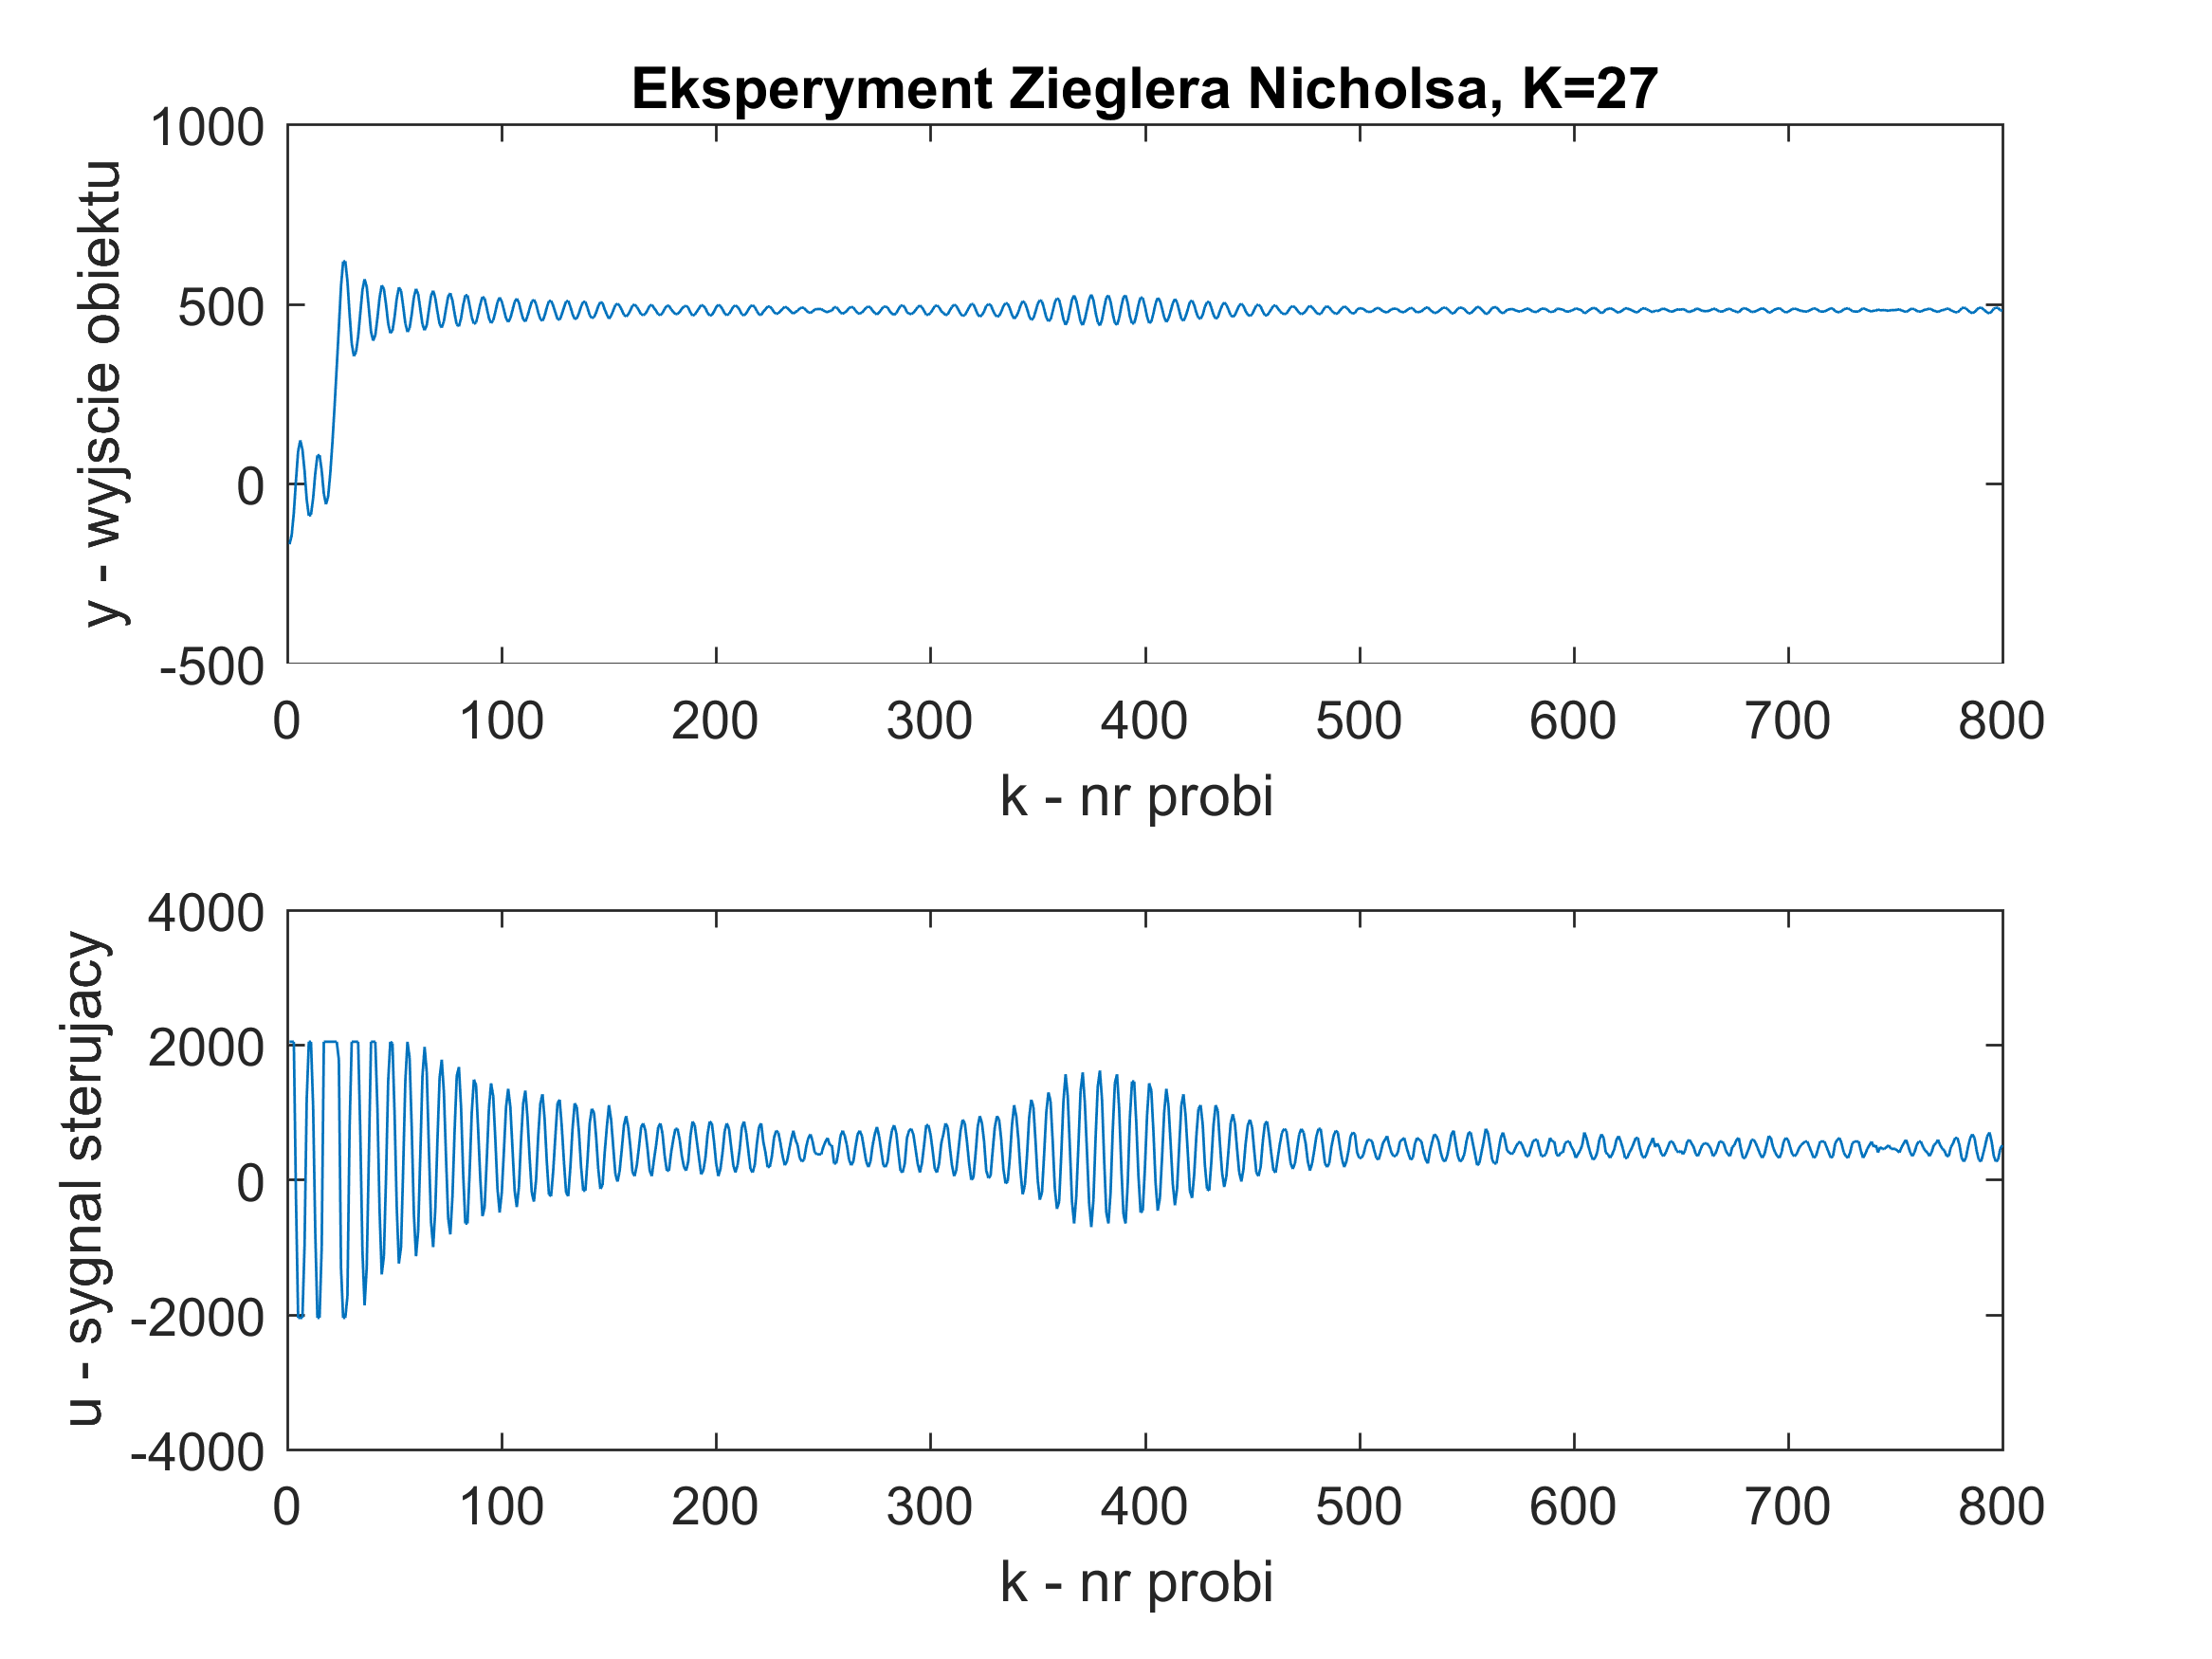
\includegraphics[width=0.9\linewidth]{EZN27}
	\caption{Wyznaczanie wzmocnienia krytycznego, $K = 27$.}
	\label{fig:EZN27}
\end{figure}

\begin{figure}[H]
	\centering
	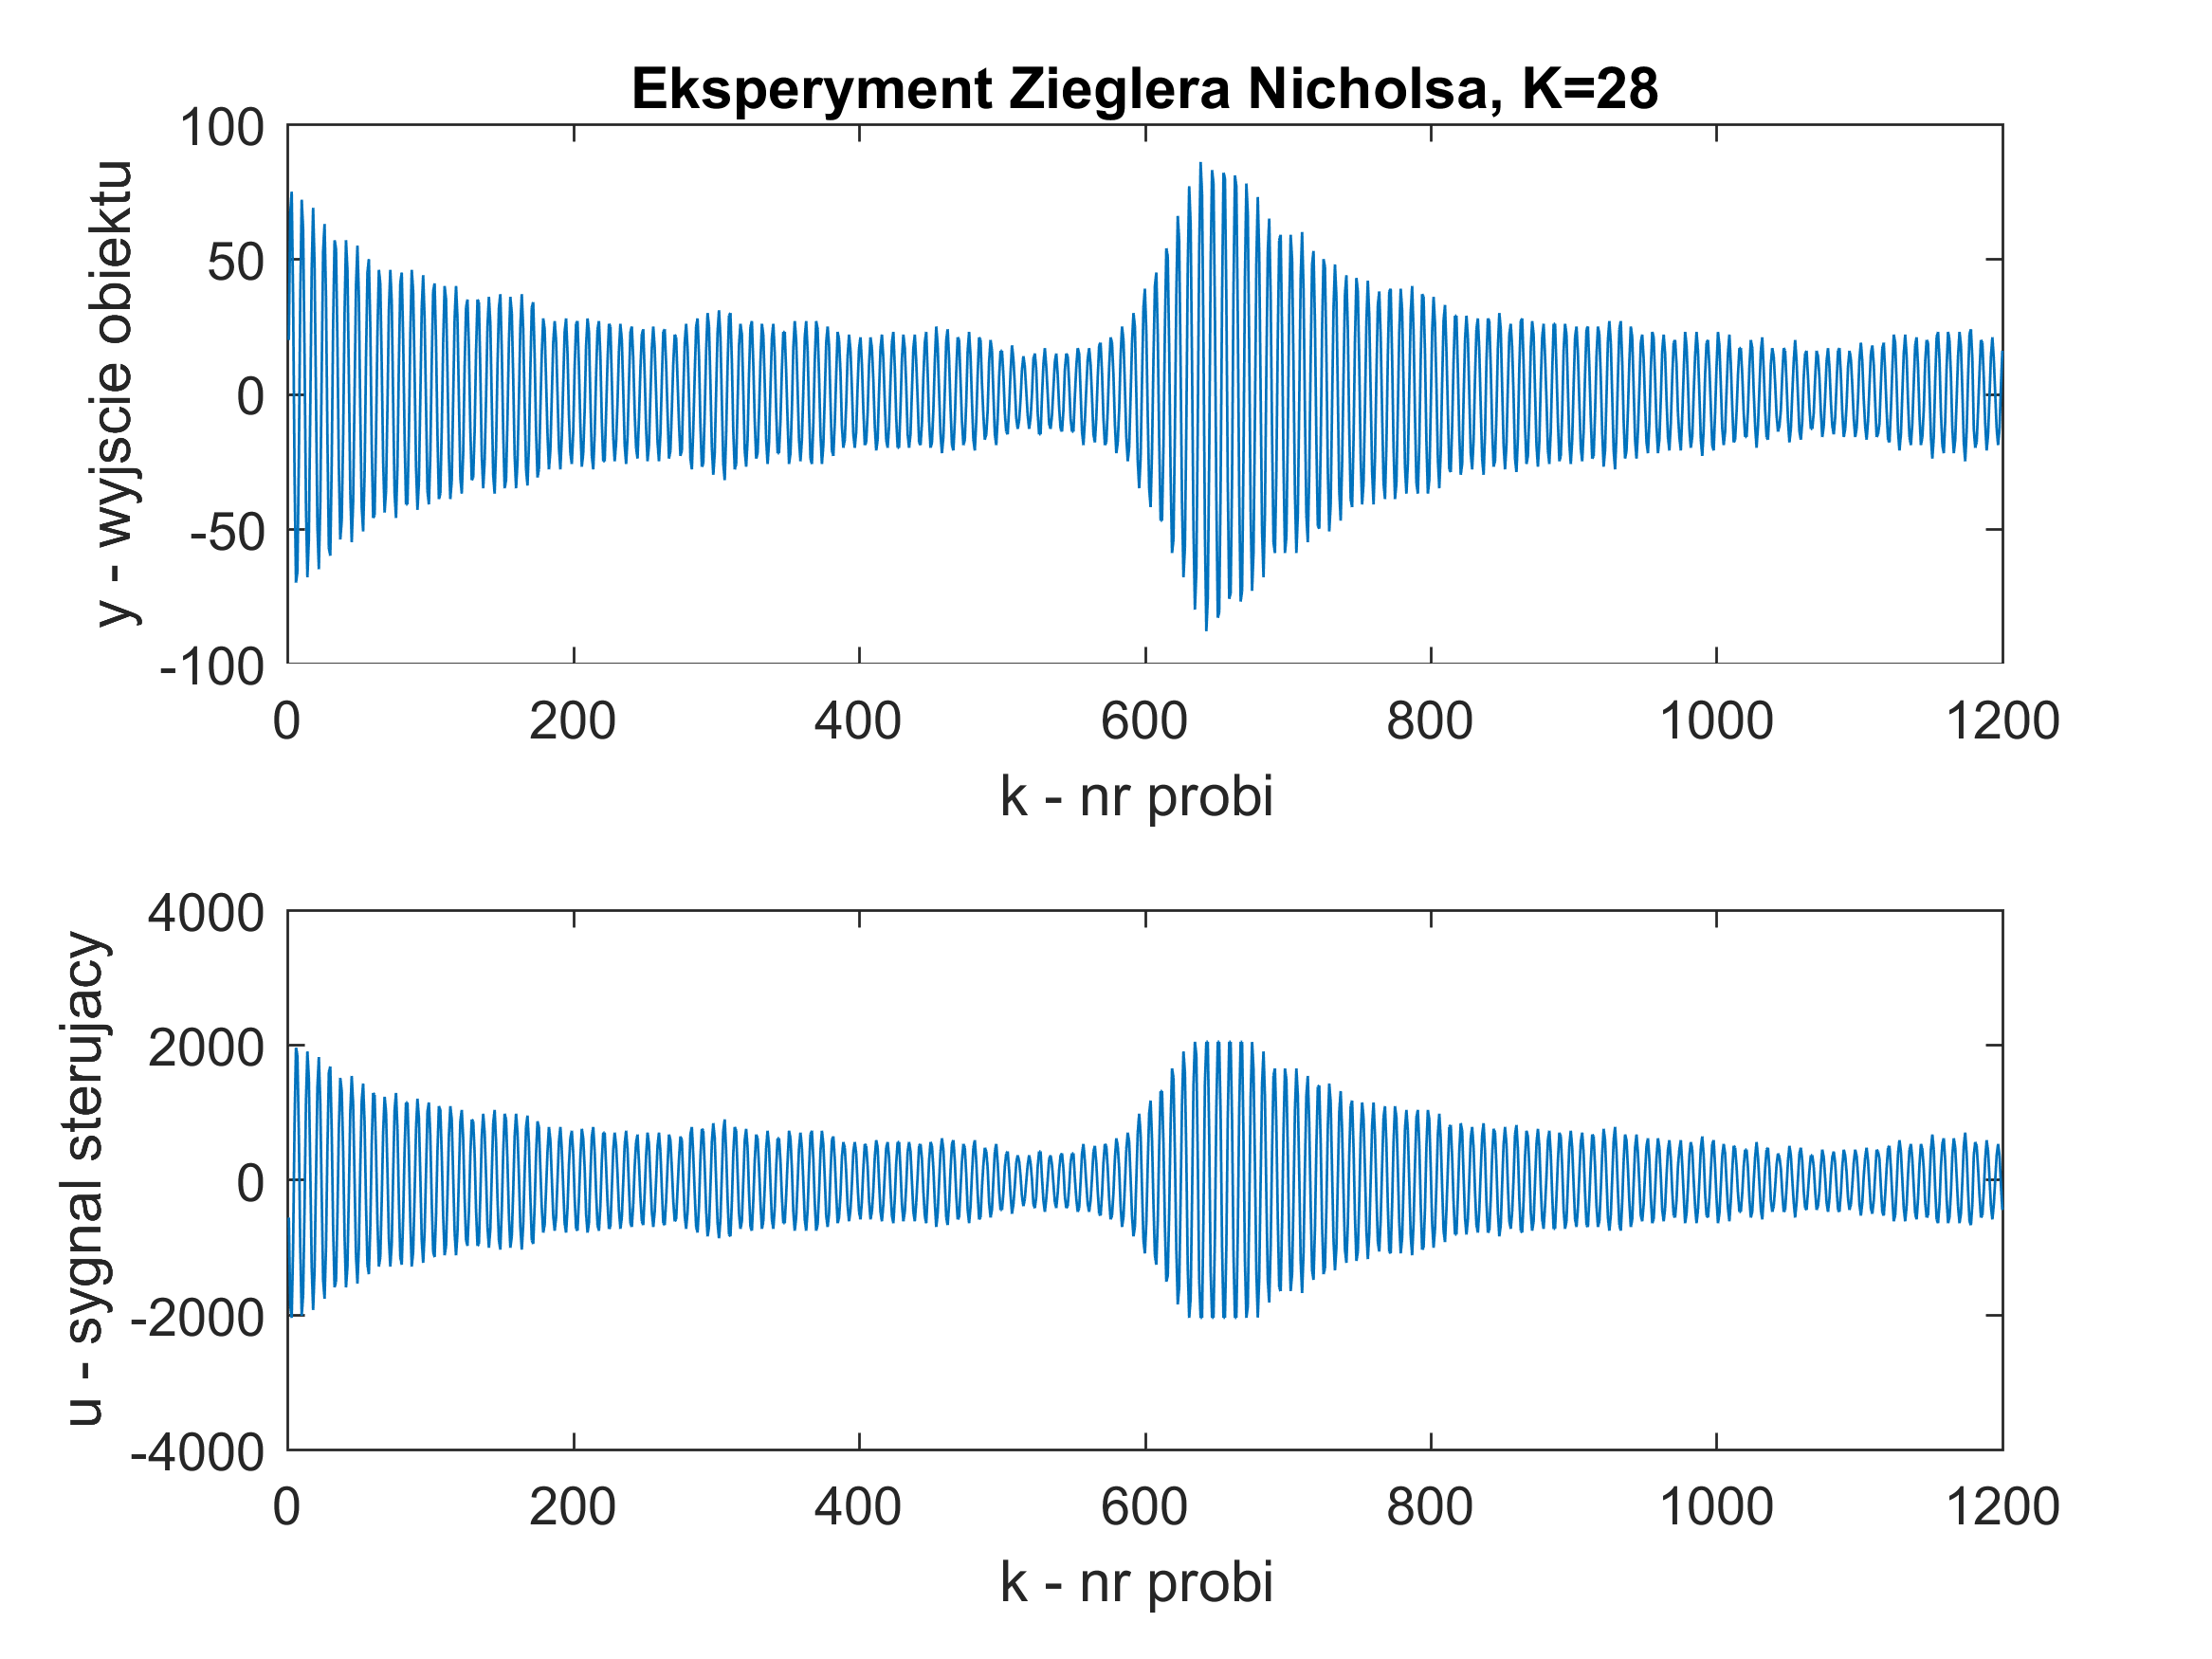
\includegraphics[width=0.9\linewidth]{EZN281}
	\caption{Wyznaczanie wzmocnienia krytycznego, $K = 28$.}
	\label{fig:EZN28}
\end{figure}

\begin{figure}[H]
	\centering
	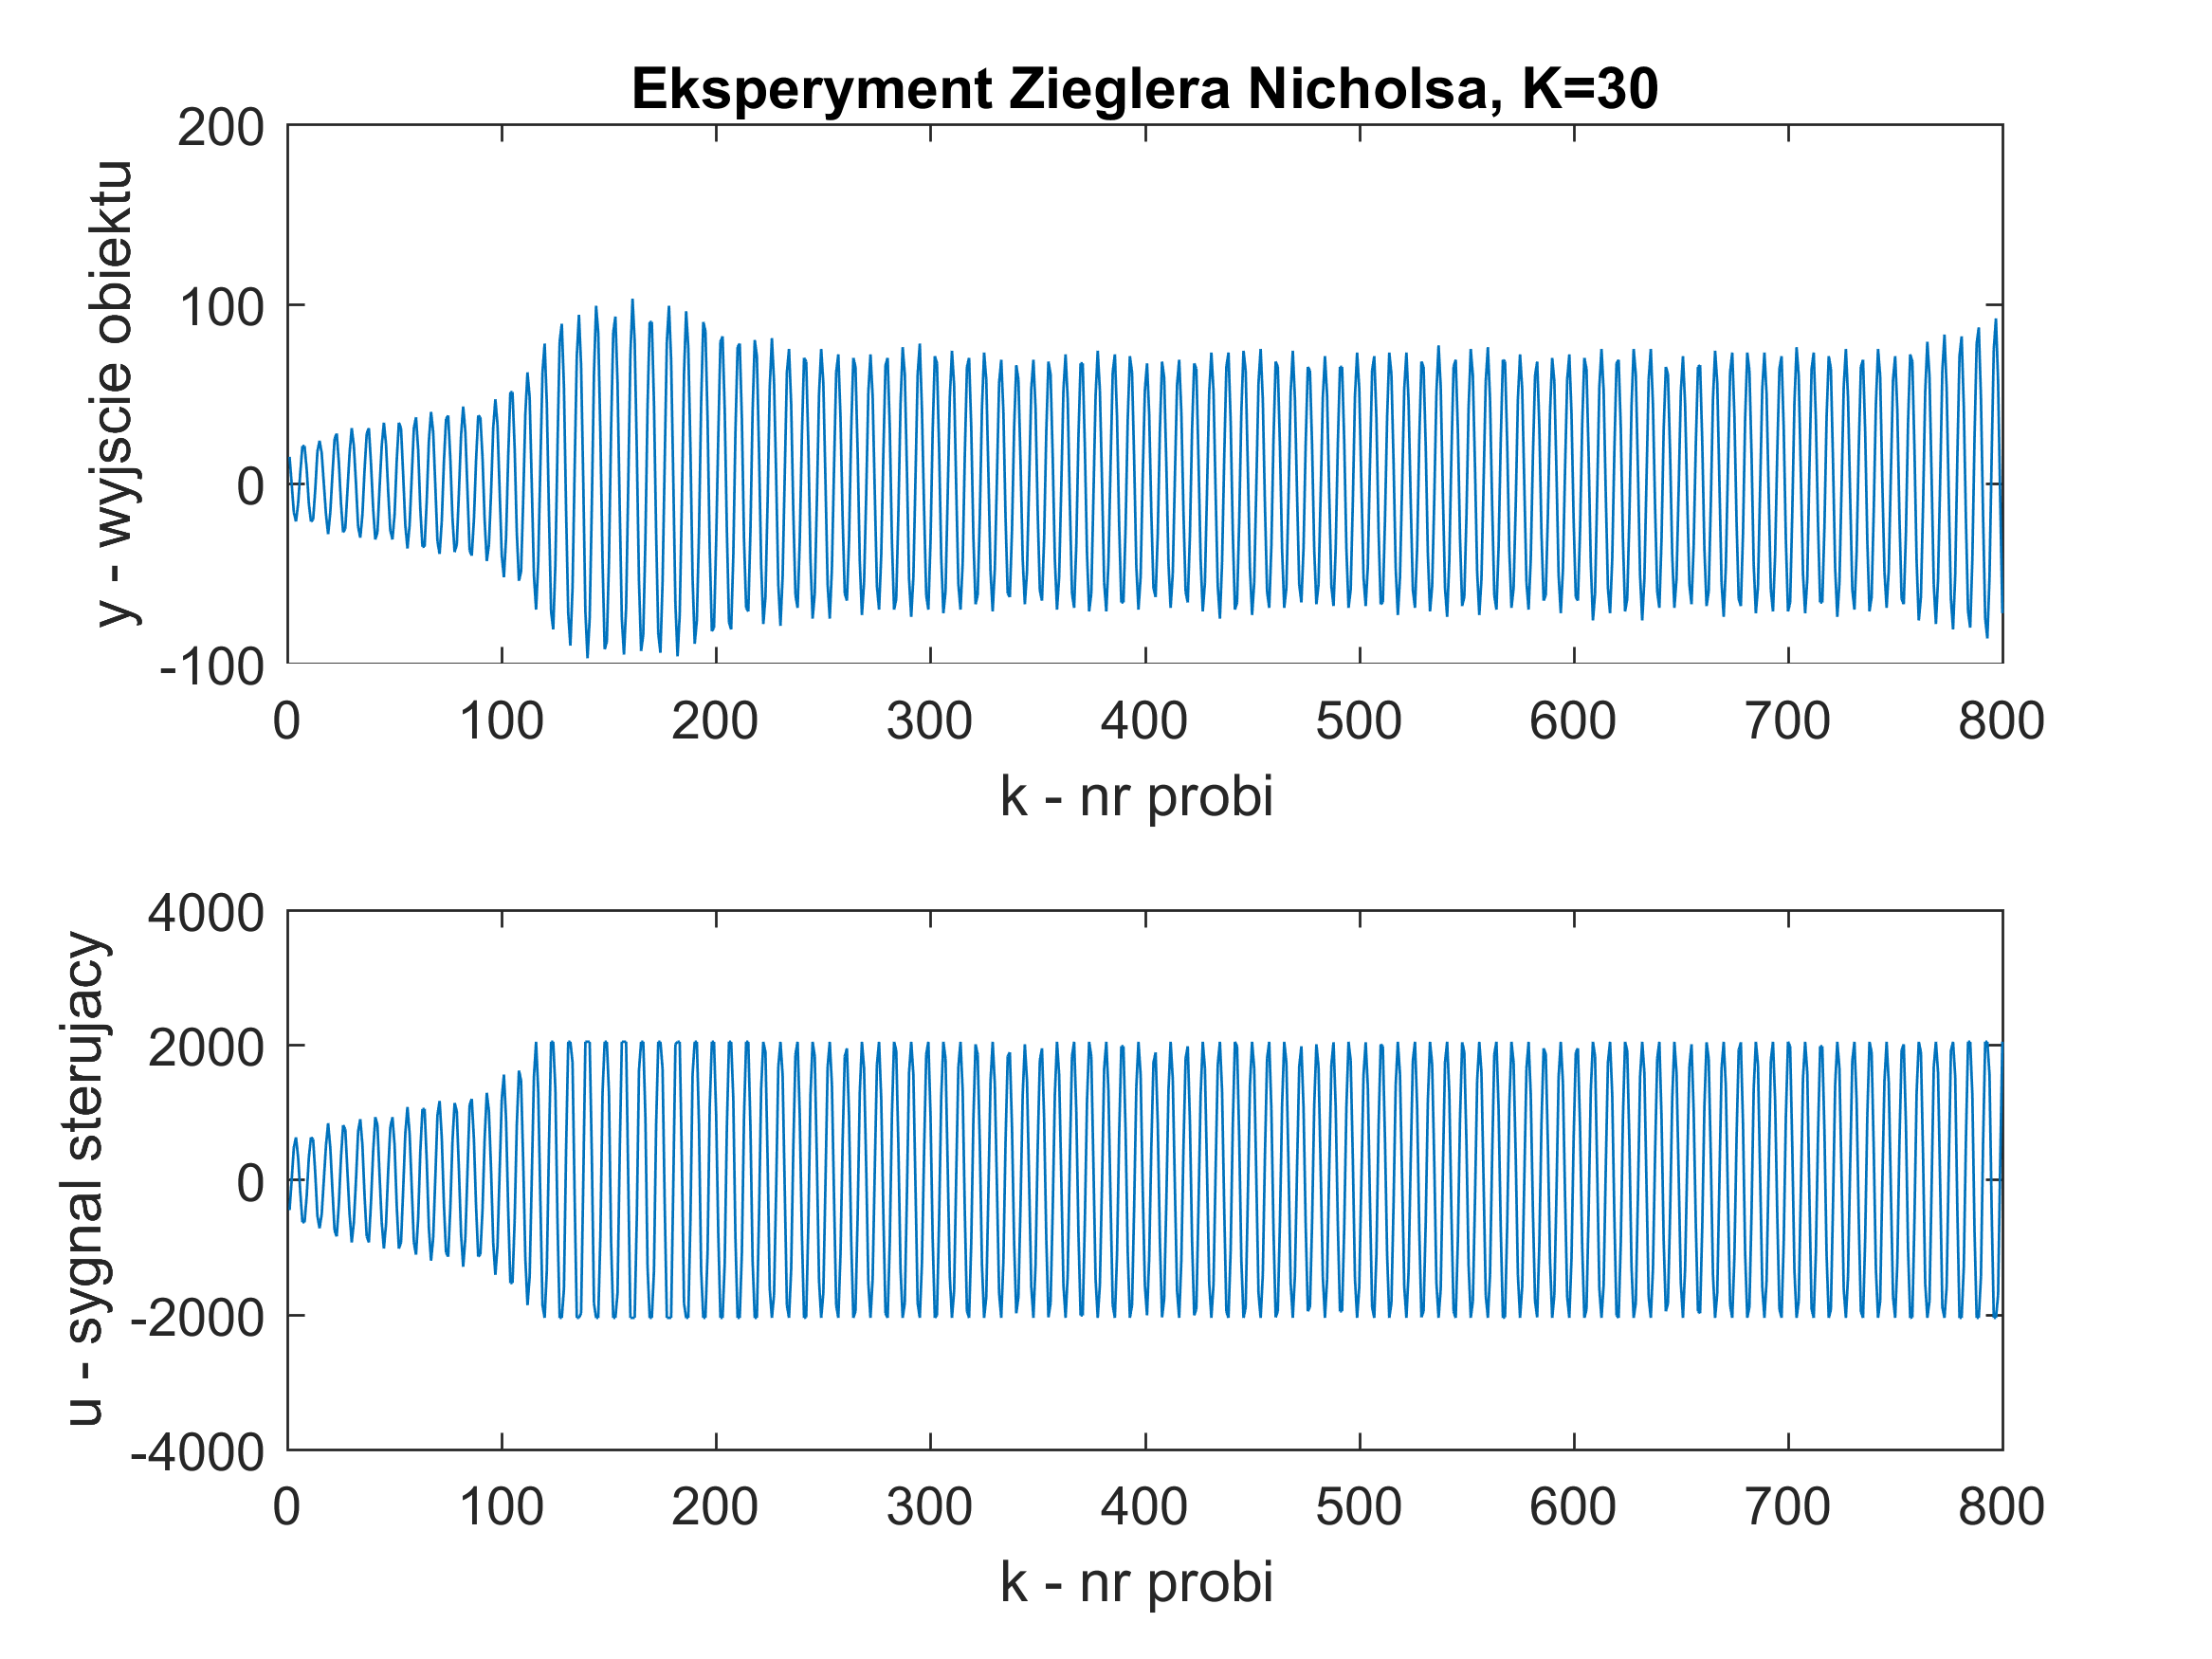
\includegraphics[width=0.9\linewidth]{EZN30}
	\caption{Wyznaczanie wzmocnienia krytycznego, $K = 30$.}
	\label{fig:EZN30}
\end{figure}

\begin{figure}[H]
	\centering
	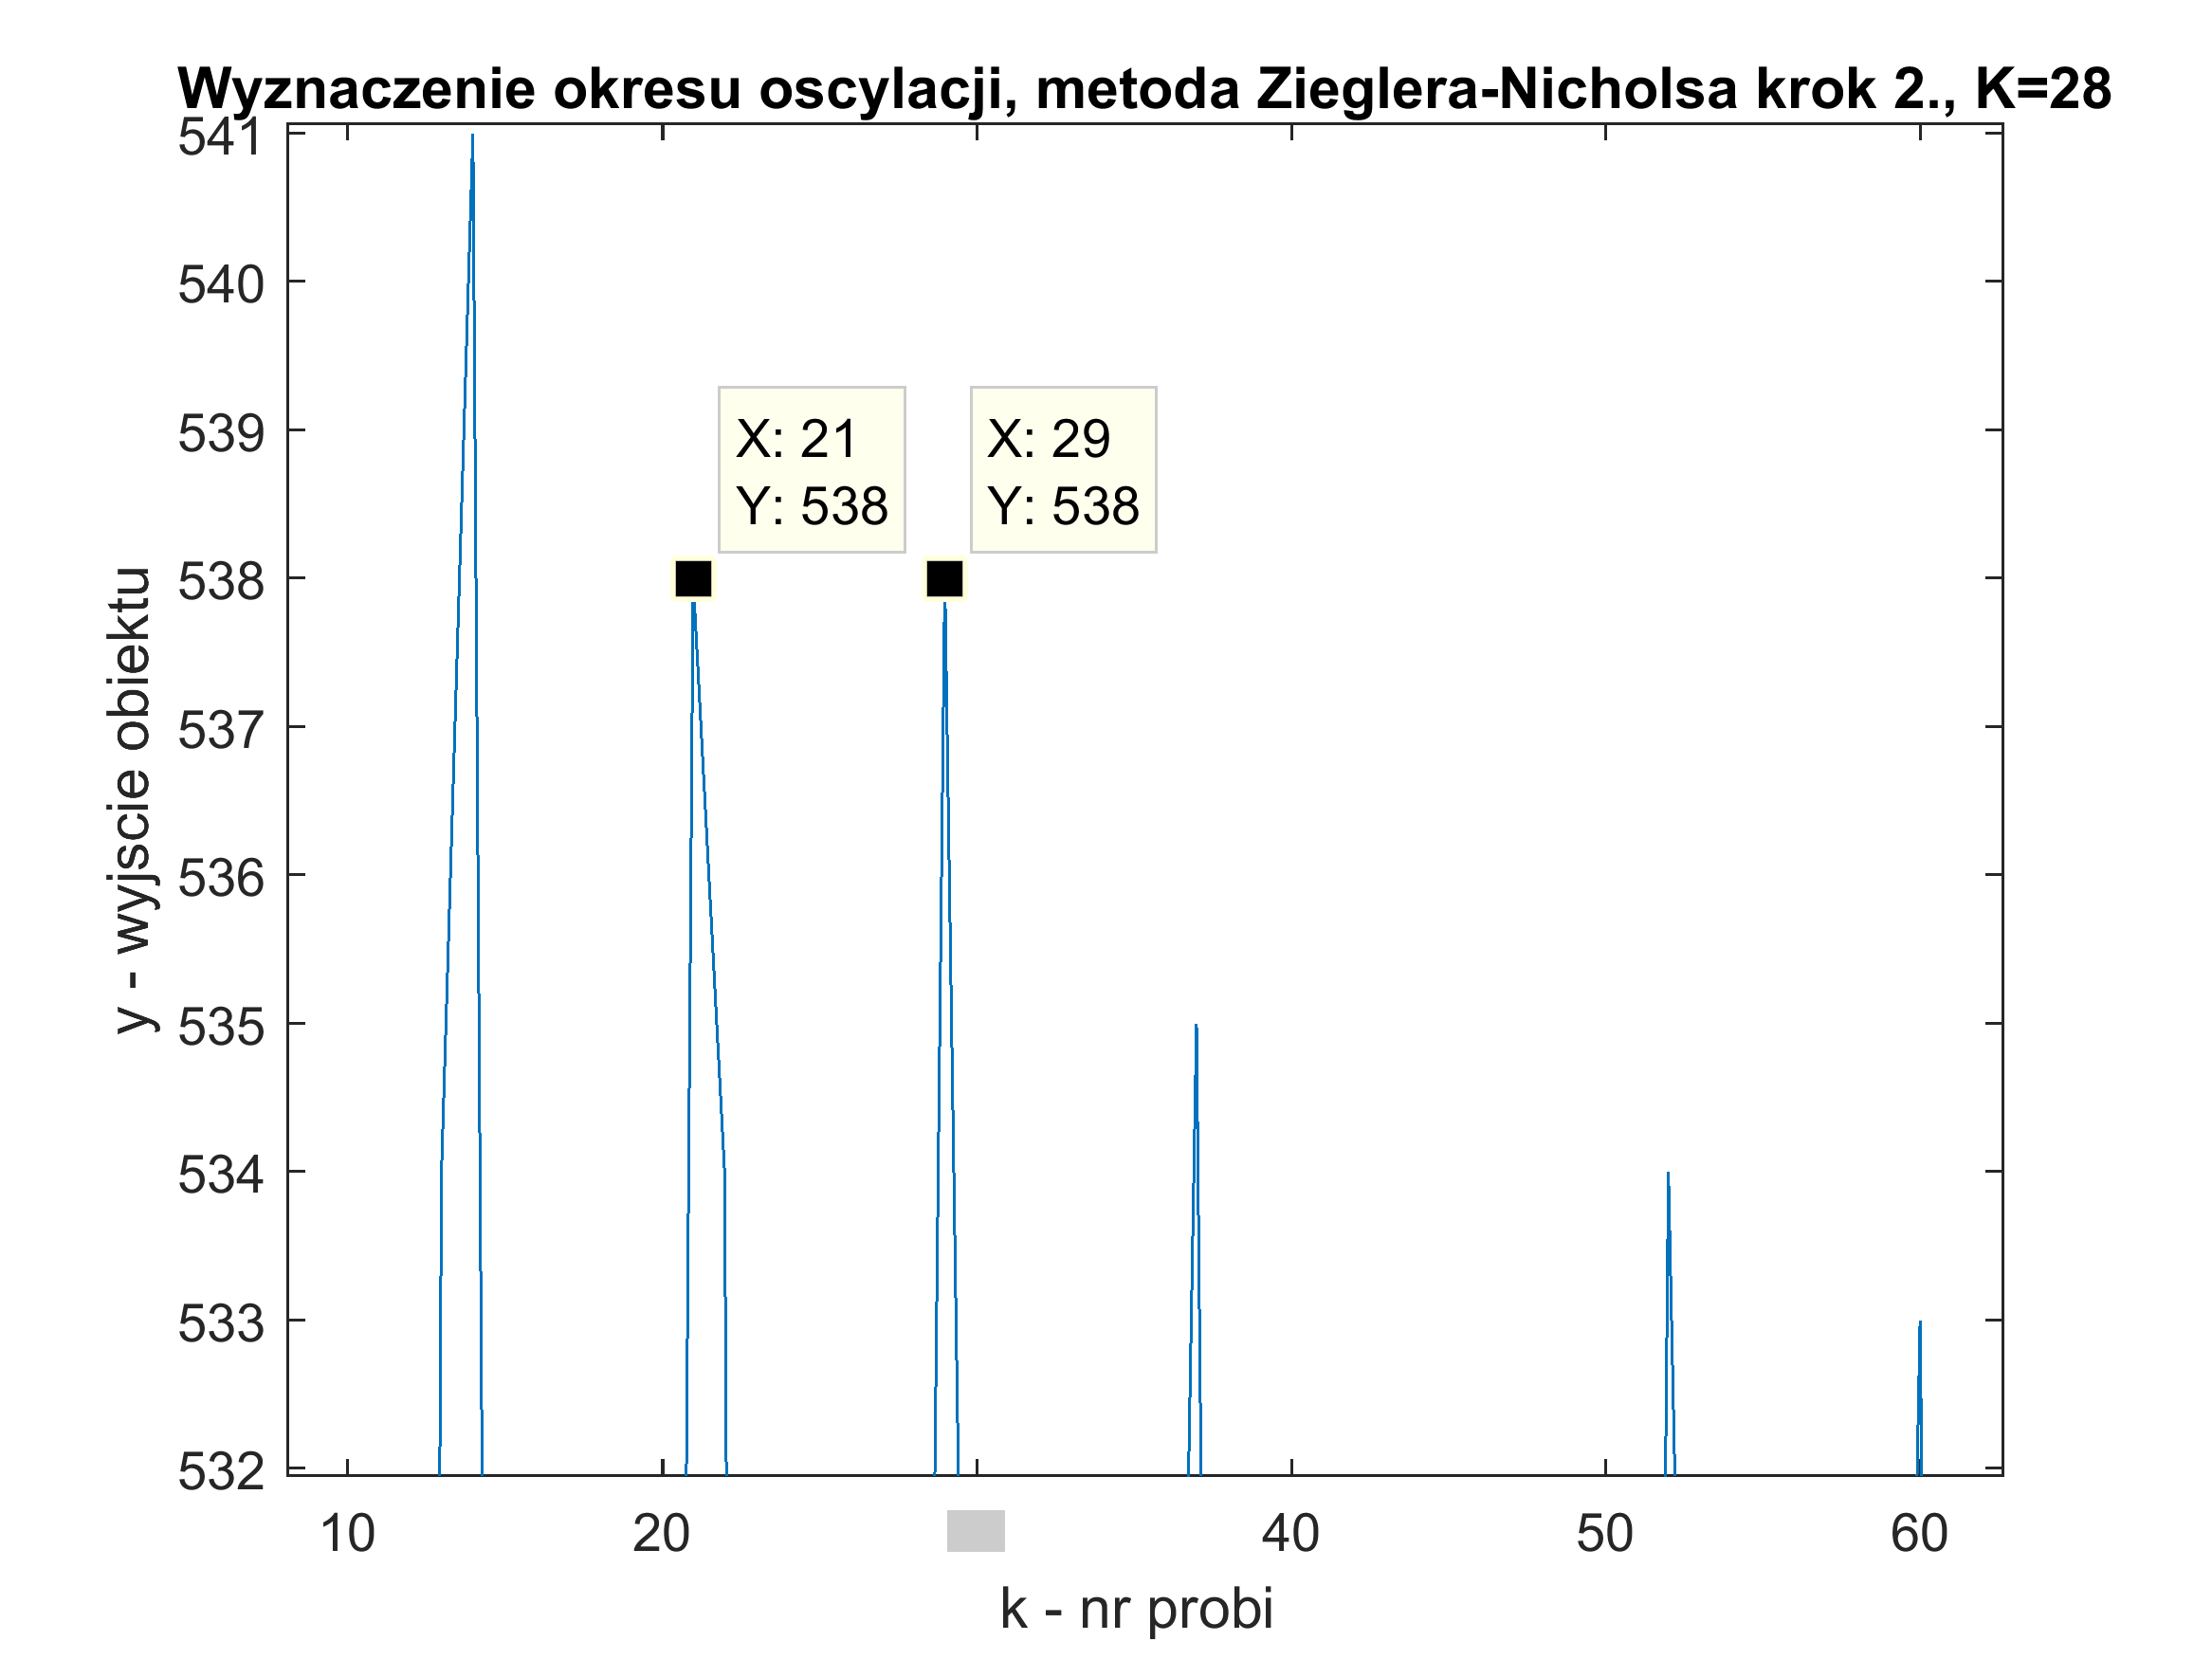
\includegraphics[width=0.9\linewidth]{Tkrytyk}
	\caption{Wyznaczanie $T_{u}$}
	\label{fig:Tkrytyk}
\end{figure}


Nastawy pełnego regulatora PID to:
\[K = 0,6\cdot K_{u} = 16,8\]
\[T_{i} = \frac{T_{u}}{2,0} = 0,2\]
\[T_{d} = \frac{T_{u}}{8} = 0,05\]

Uzyskane przebiegi wskazują na to, że regulator nie jest optymalny. Występują przeregulowanie i oscylacje. 

\begin{figure}[H]
	\centering
	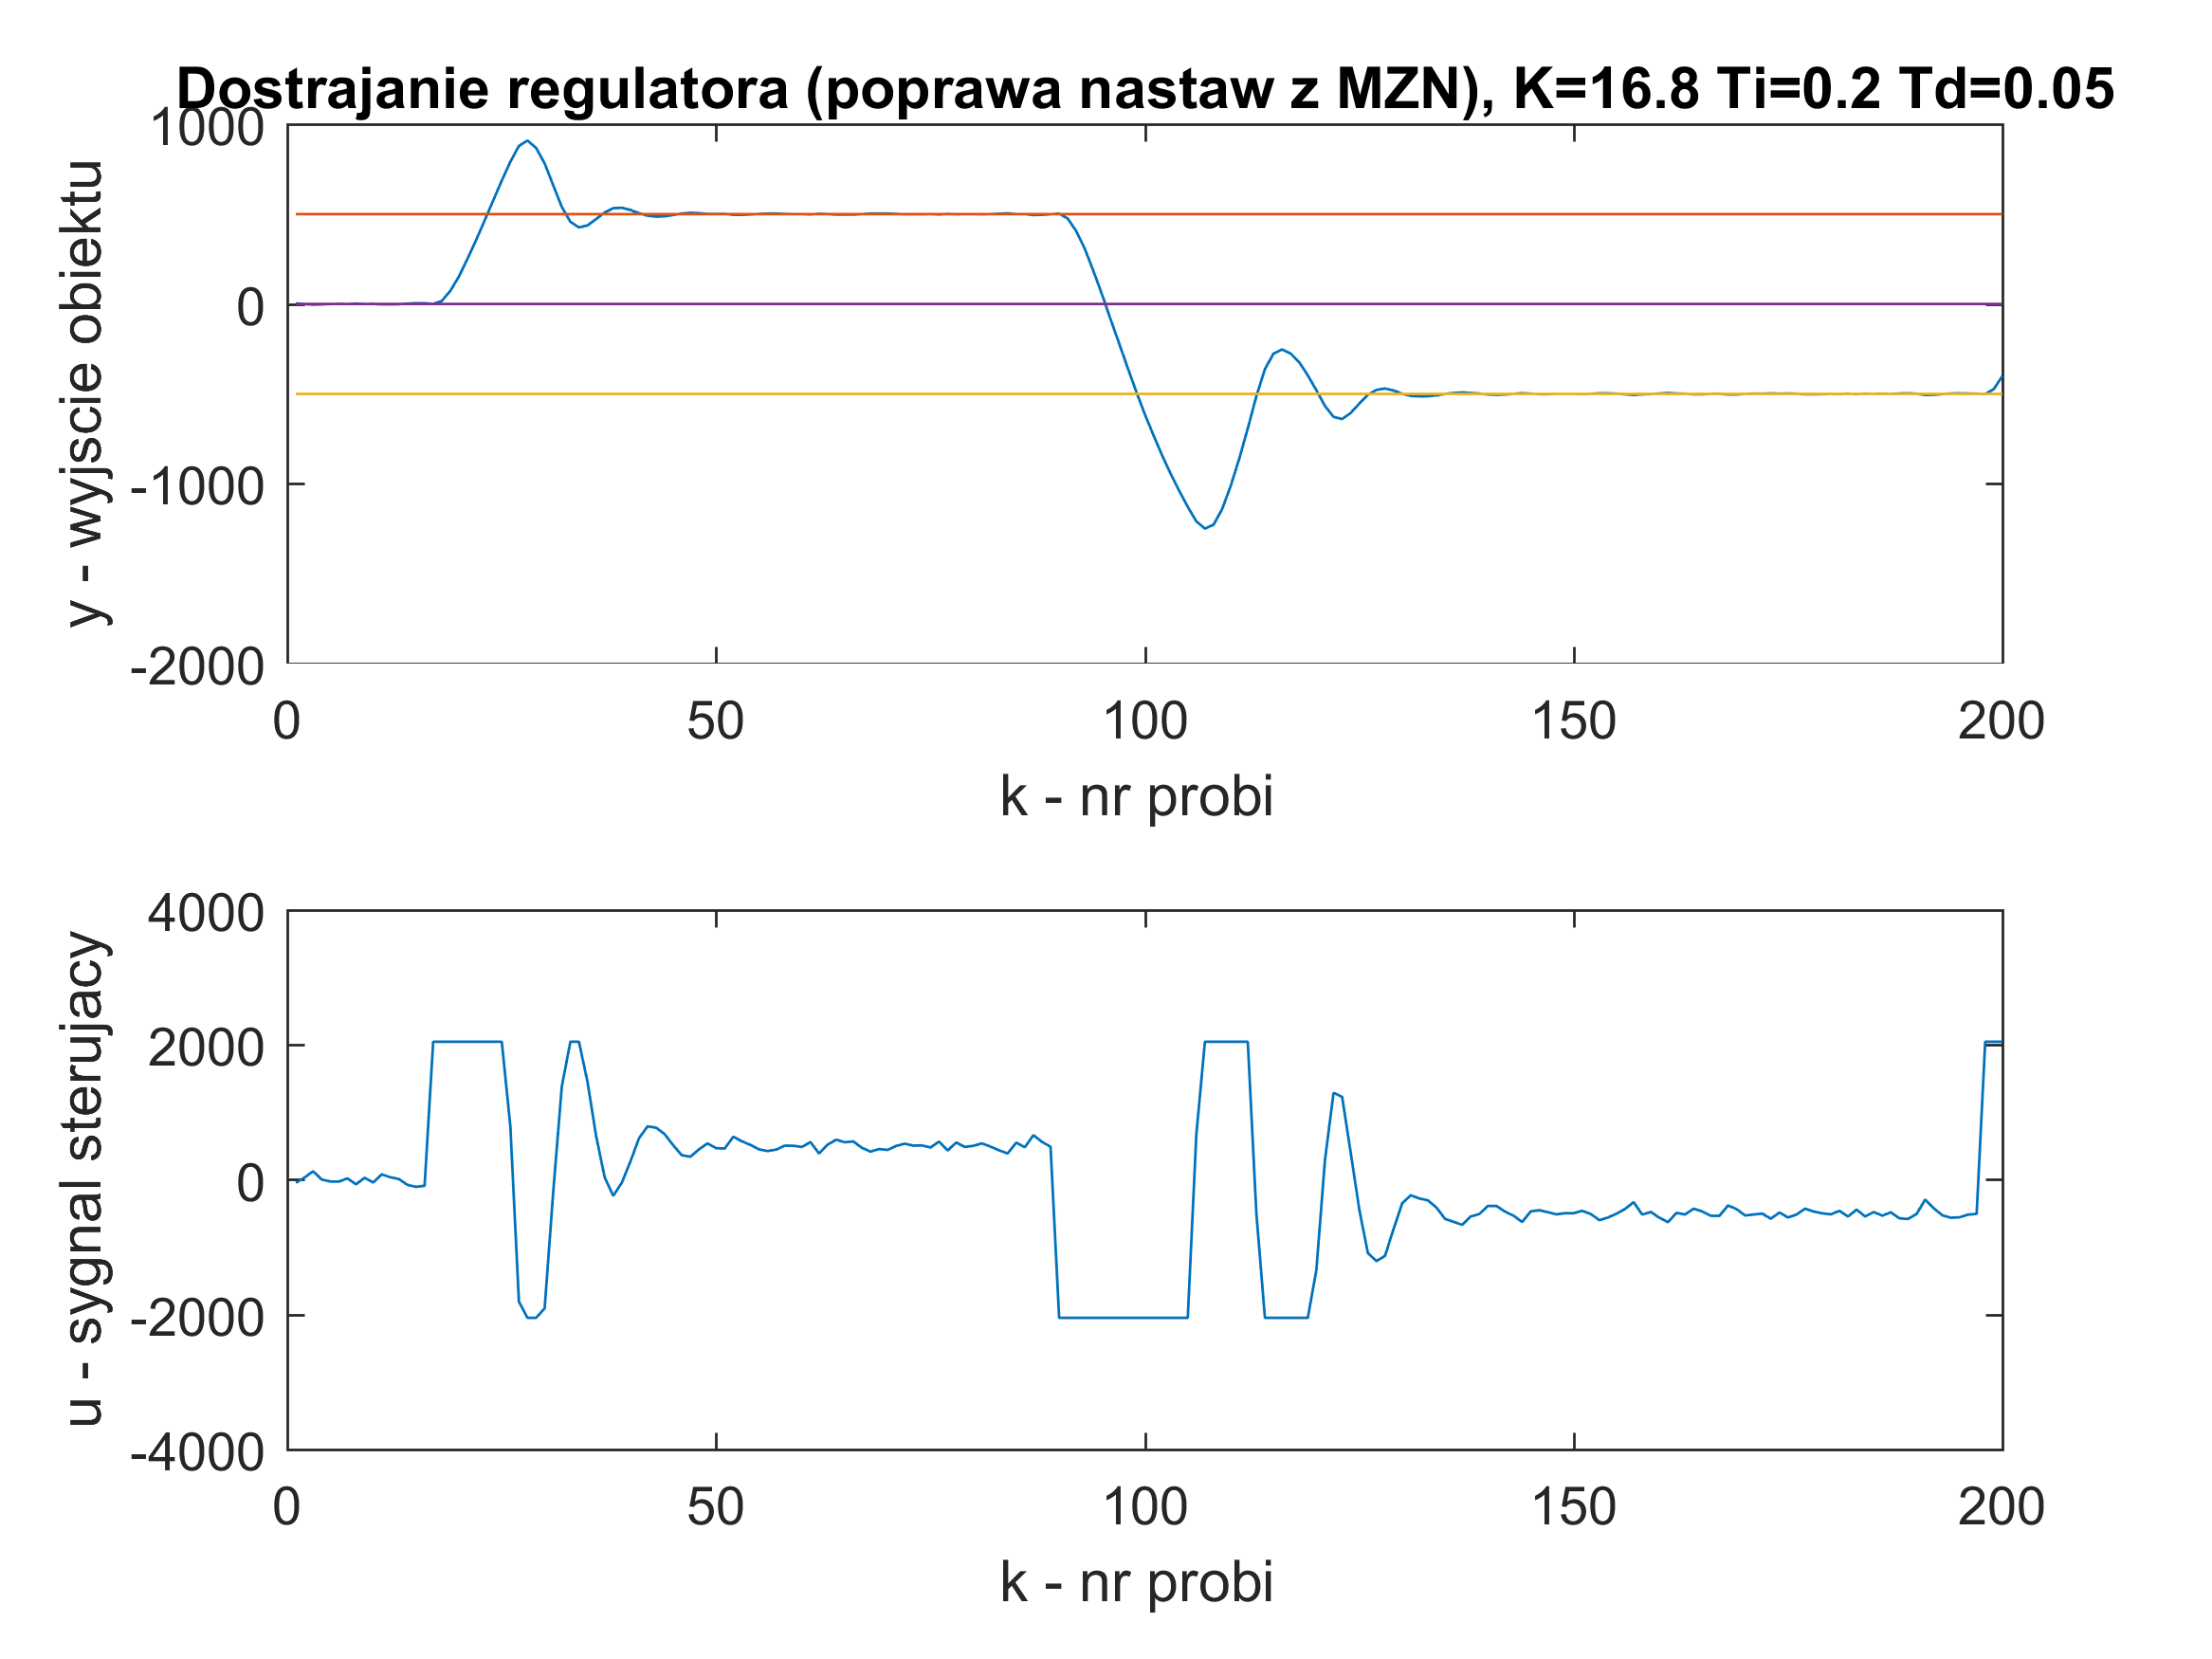
\includegraphics[width=0.9\linewidth]{zn_bez}
	\caption{Trajektoria sygnału wyjściowego dla regulatora PID wyznaczonego metodą Zieglera-Nicholsa}
	\label{fig:znbez}
\end{figure}

\subsection{Wyznaczanie parametrów metodą inżynierską}
Metoda inżynierska pozwala na eksperymentalny dobór wartości parametrów regulatora PID. Składa się ona z czterech kroków. \\

1. Wyznczenie wzmocnienia\\
Jest to etap identyczny jak w przypadku metody Zieglera Nicholsa. Za pomocą regulatora proporcjonalnego wprowadza się obiekt w stan niegasnących oscylacji. Wzmocnienie jakie miał owy regulator zwane jest wzmocnieniem krytycznym i oznaczane jest $K_{u}$. 

2. Dobór parametru $T_{I}$\\
Przyjmując, że parametr $K=0,5\cdot K_{u}$ stopniowo dobiera się parametr $T_{I}$, tak aby regulator lepiej spełniał kryterium oceny.

3. Dobór parametru $T_{D}$\\
Przyjmując parametry $K$ i $T_{I}$ wyznaczone w poprzednich krokach stroi się regulator zmieniając eksperymentalnie wartośc parametru $T_{D}$.

4. Dostrojenie regulatora\\
\subsubsection{Krok 1. - Wyznaczenie $K$}
Krok ten jest identyczny z pierwszym krokiem w metody Zieglera-Nicholsa. W punkcie \ref{krytyk} wyznaczone zostało $K_{u}=28$. Zgodnie z wzorem $K=0,5 \cdot K_{u}$ przyjęte zostało wzmocnienie równe: $K=14$.
\subsubsection{Krok 2. - Dobór parametru $T_{I}$}

Metoda inżynierska charakteryzuje się eksperymentalnym sposobem wyznaczania parametrów regulatora. Zgodnie z założeniami chcemy, aby nasz regulator posiadał zerowy uchyb ustalony, szybki czas regulacji i ograniczone przesterowanie. \\
Przy doborze parametru $T_{I}$ wyłączony został człon różniczkujący, czyli:\\
\[u(k)=u_{P}(k)+u_{I}(k)\]
Przeprowadzone zostały eksperymenty dla $T_{I}$ równego kolejno: $T_{I}=0,2$ , $T_{I}=2$ , $T_{I}=1,8$ , $T_{I}=2,2$ , $T_{I}=3,0$ i $T_{I}=20$.
\begin{figure}[H]
	\centering
	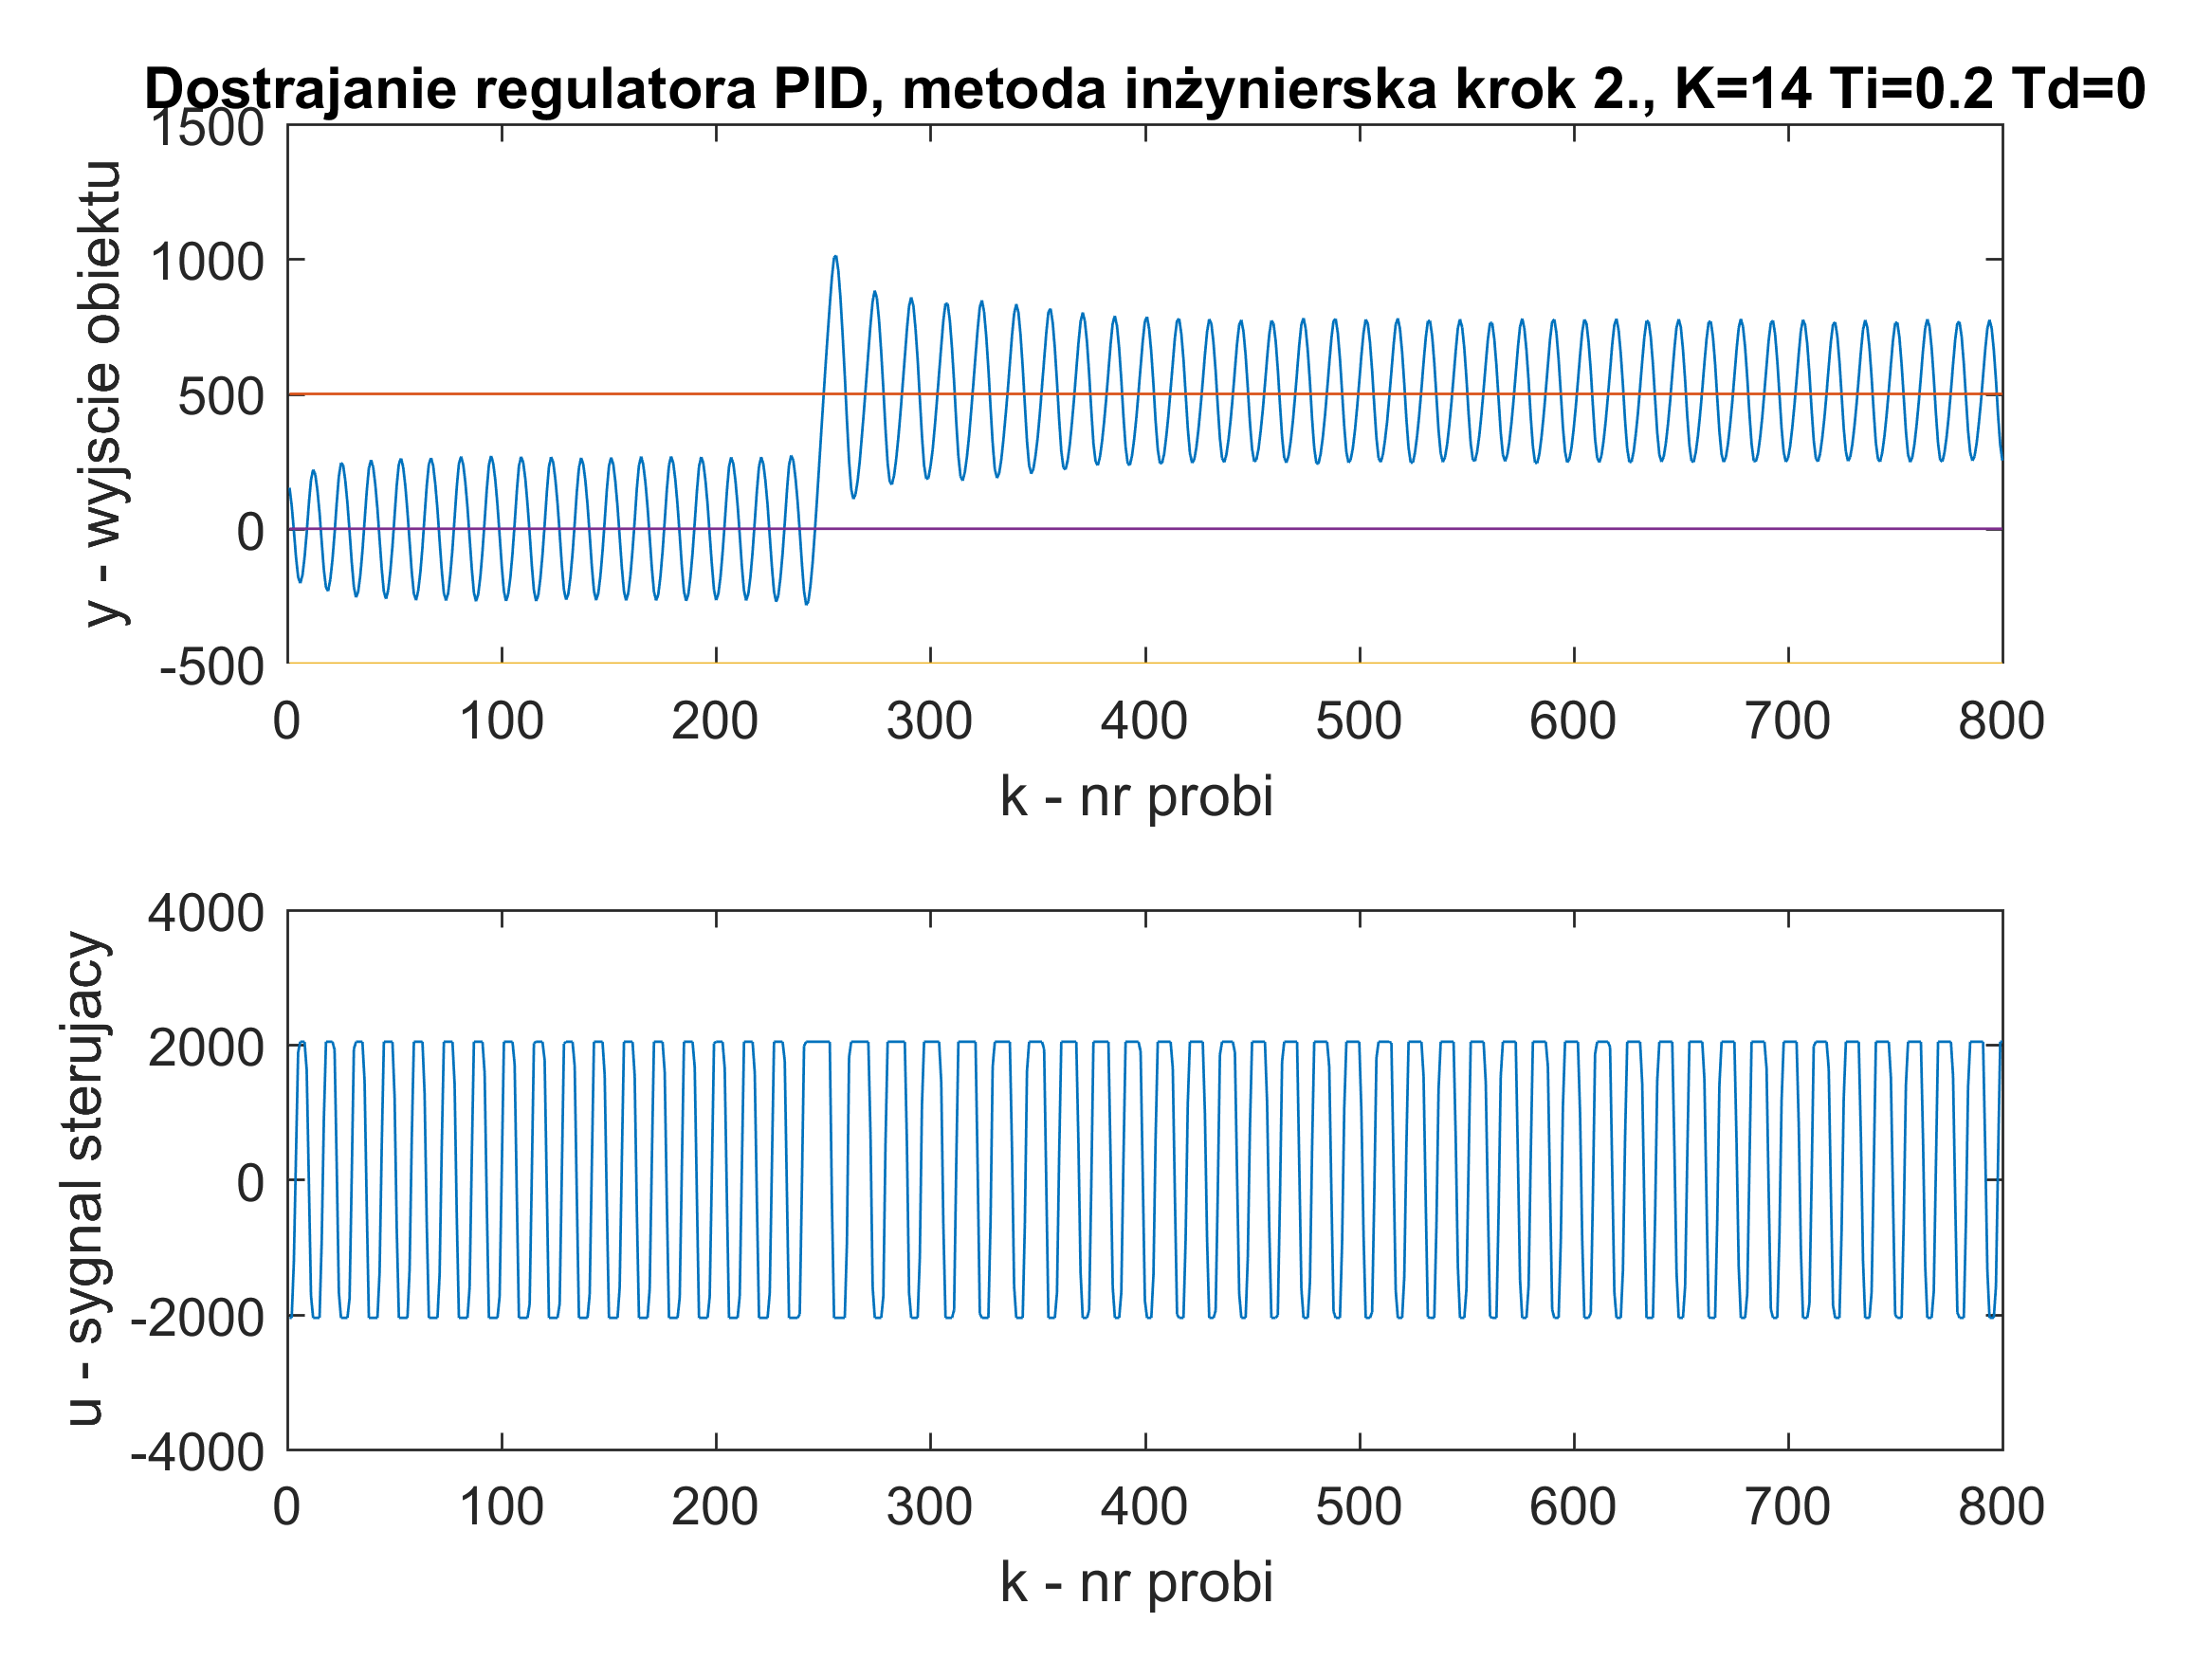
\includegraphics[width=0.9\linewidth]{MI_ti200}
	\caption{Wyjście obiektu przy $T_{I}=0,2$ - czas zdwojenia}
	\label{fig:MI_ti200}
\end{figure}
\begin{figure}[H]
	\centering
	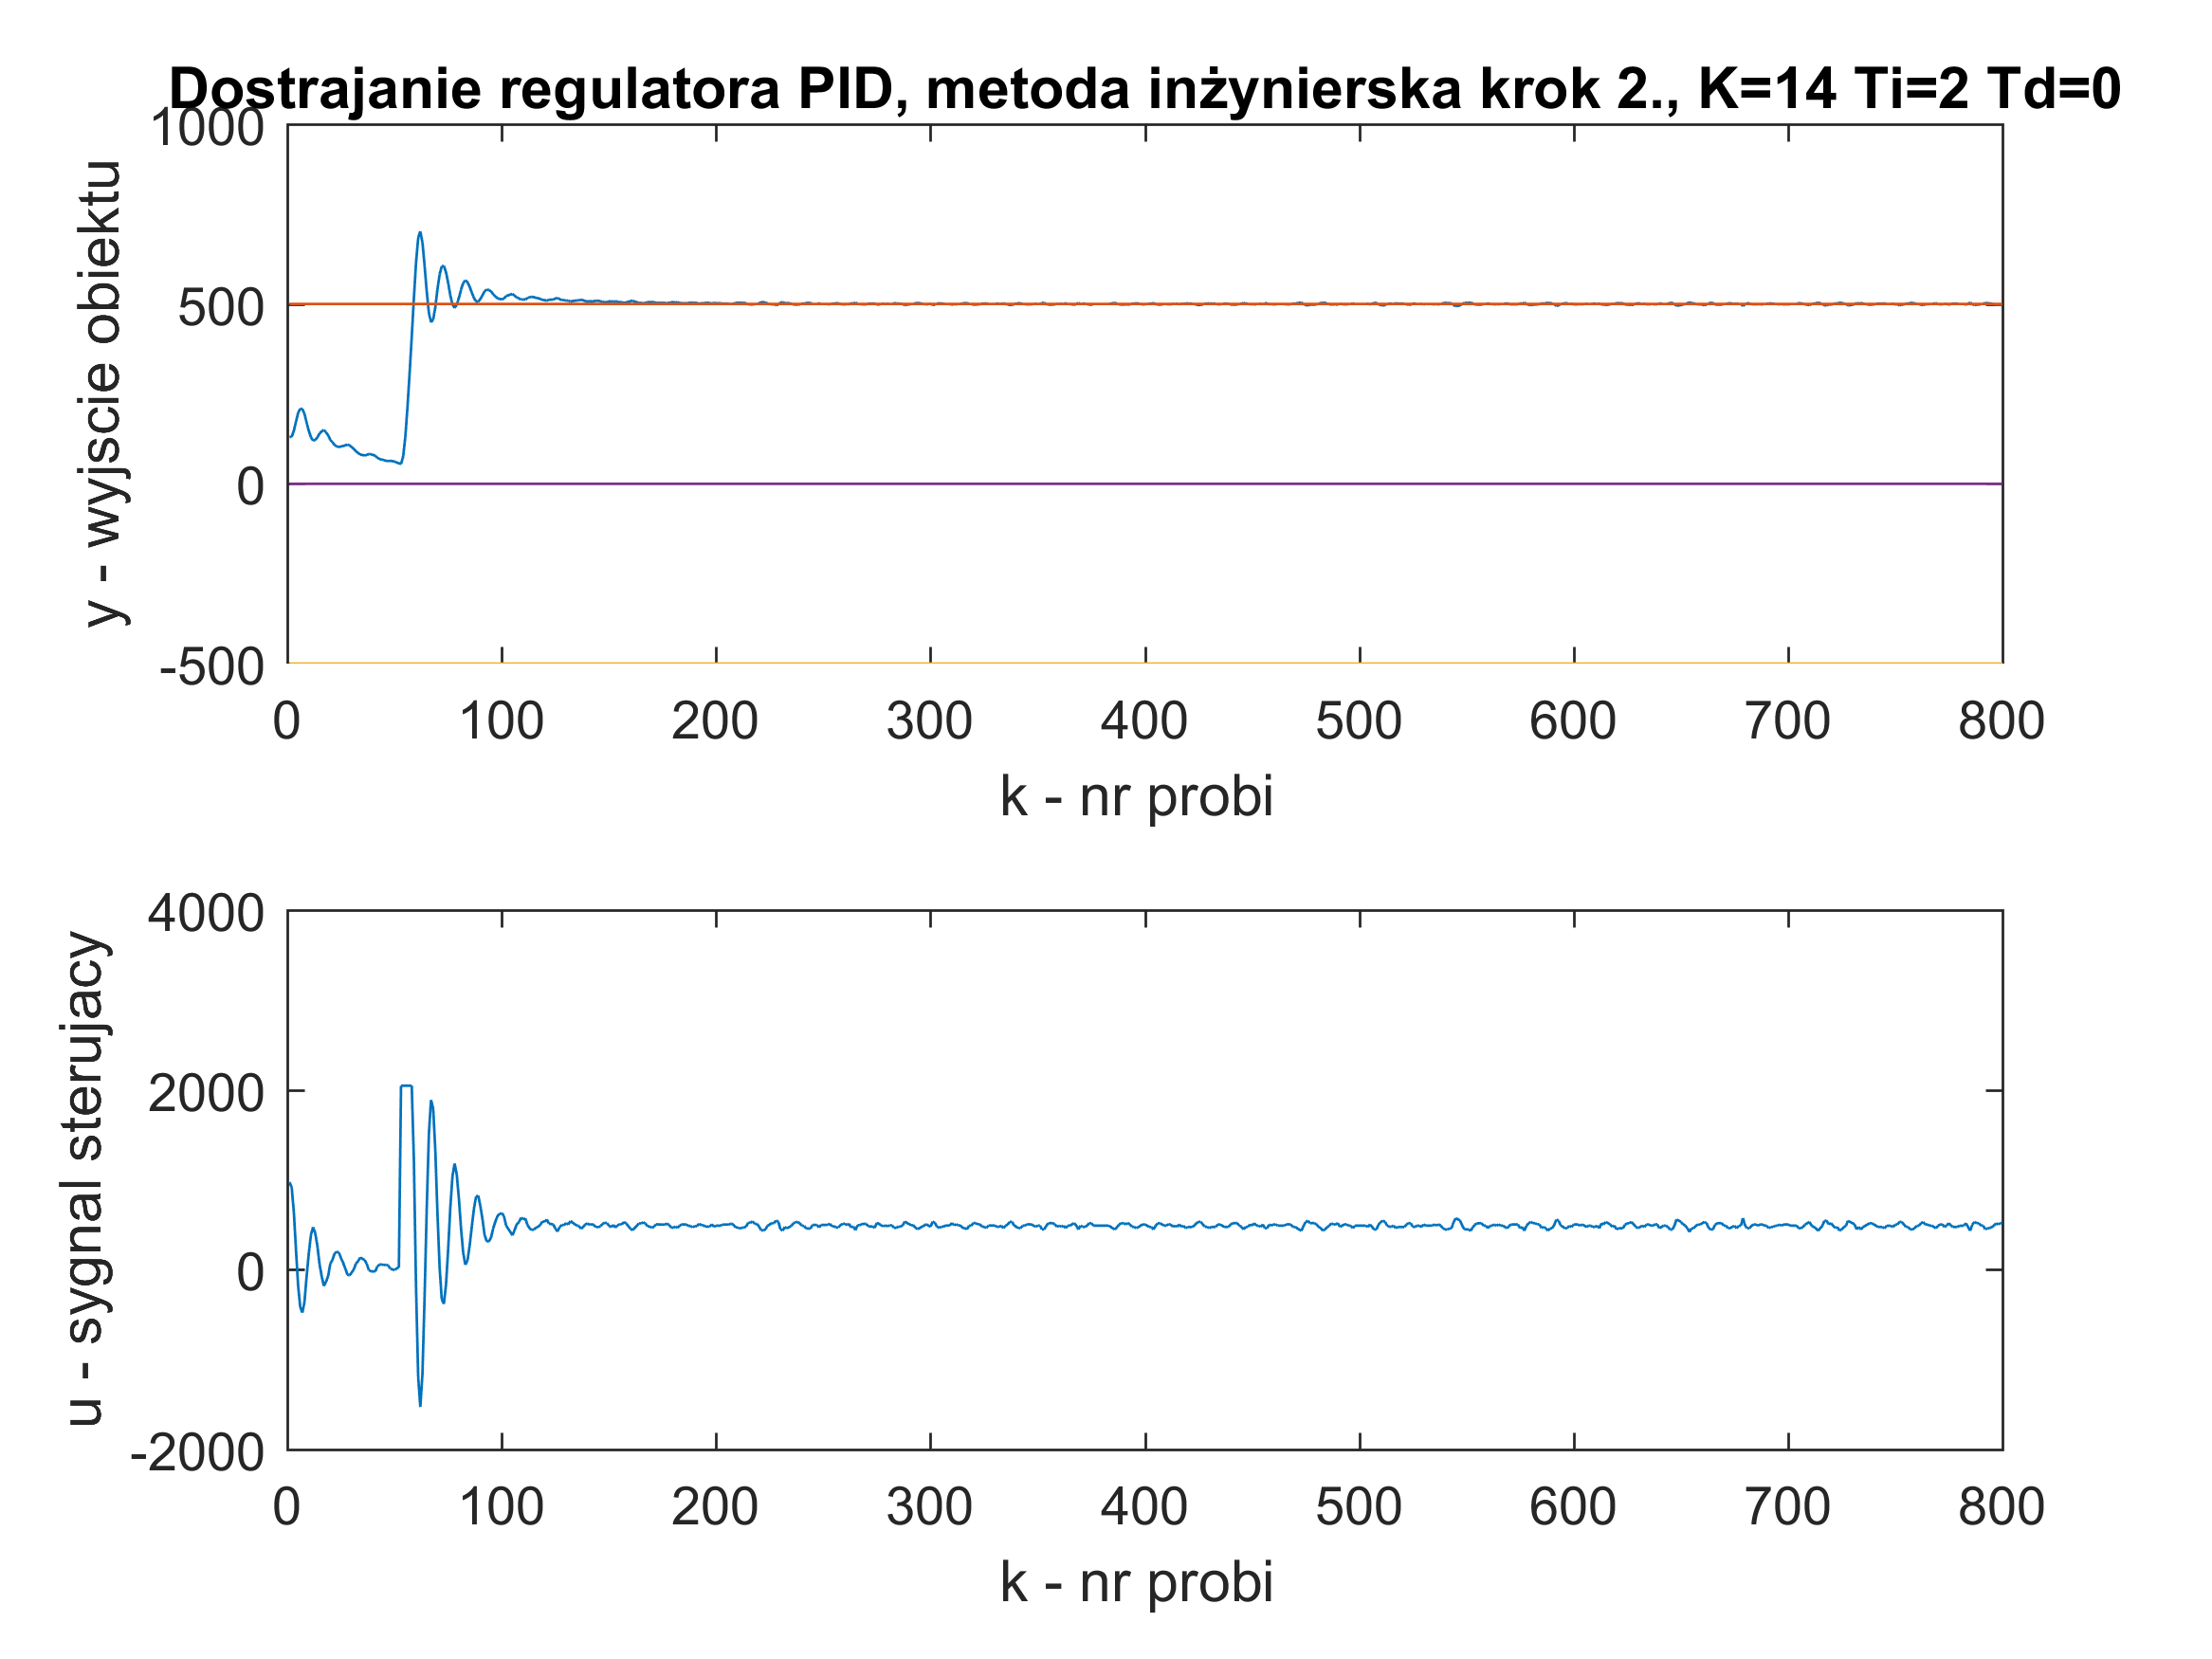
\includegraphics[width=0.9\linewidth]{MI_ti2000}
	\caption{Wyjście obiektu przy $T_{I}=2,0$ }
	\label{fig:MI_ti2000}
\end{figure}
\begin{figure}[H]
	\centering
	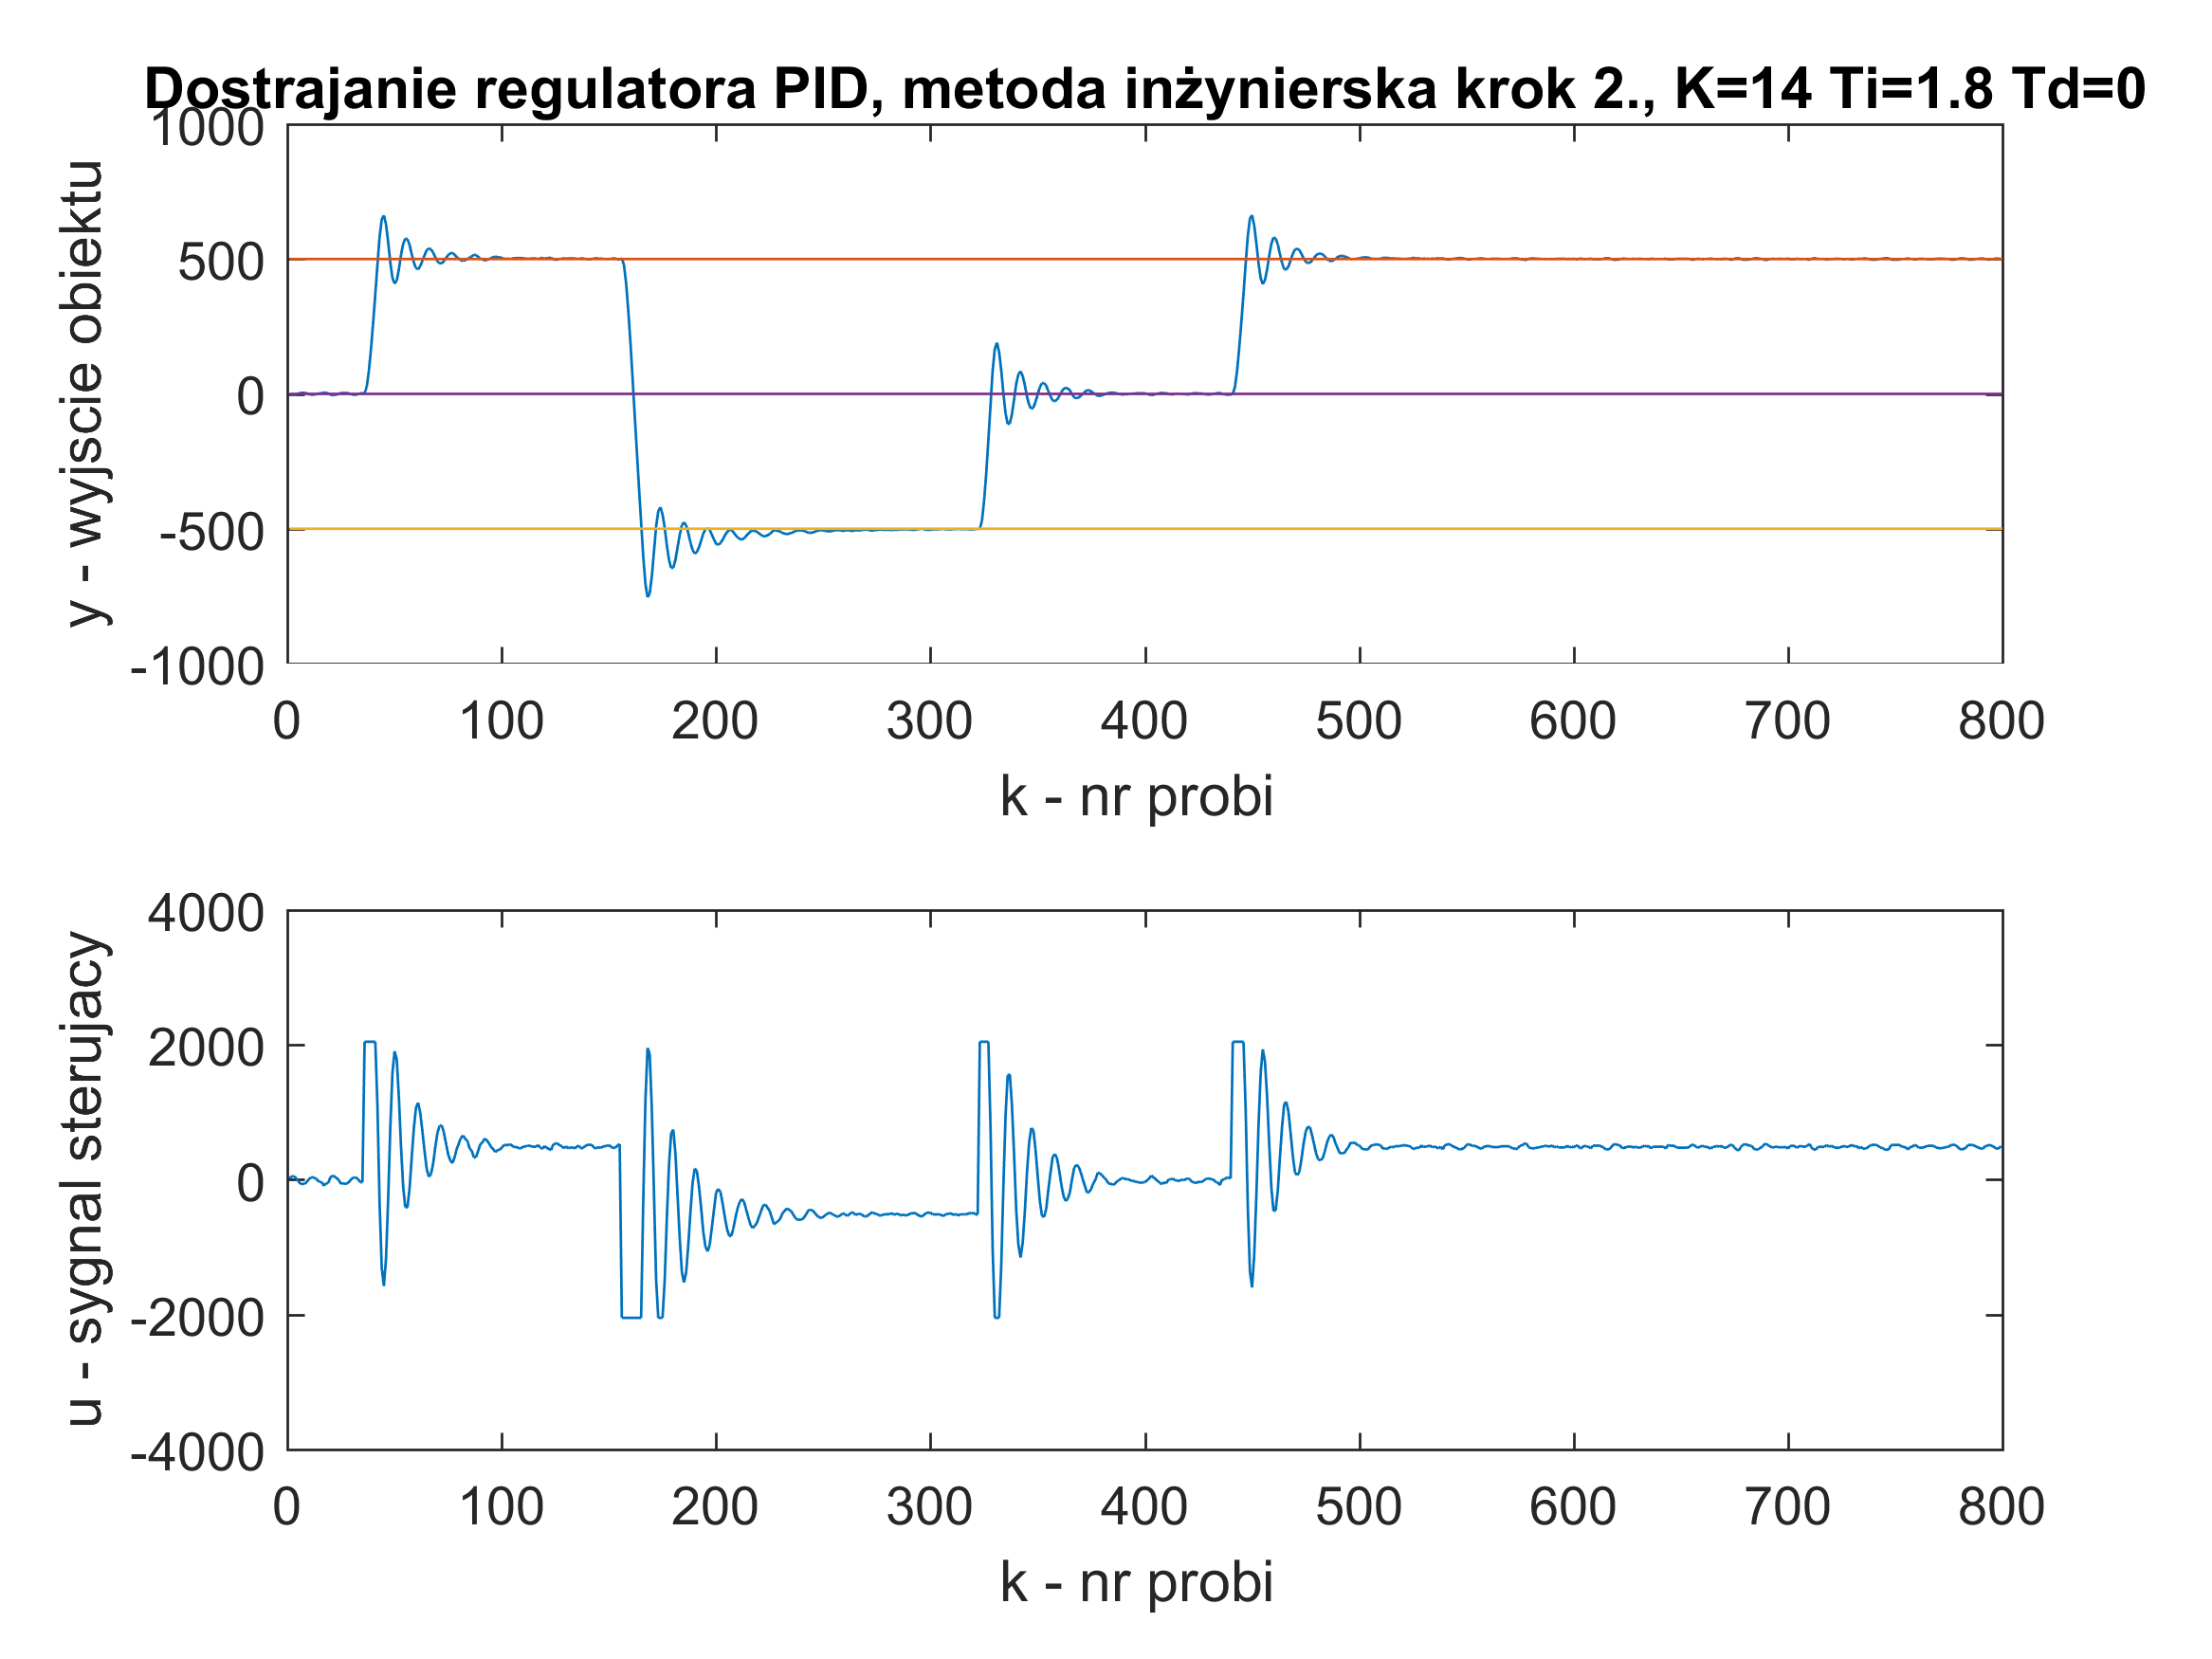
\includegraphics[width=0.9\linewidth]{MI_ti1800}
	\caption{Wyjście obiektu przy $T_{I}=1,8$ }
	\label{fig:MI_ti1800}
\end{figure}
\begin{figure}[H]
	\centering
	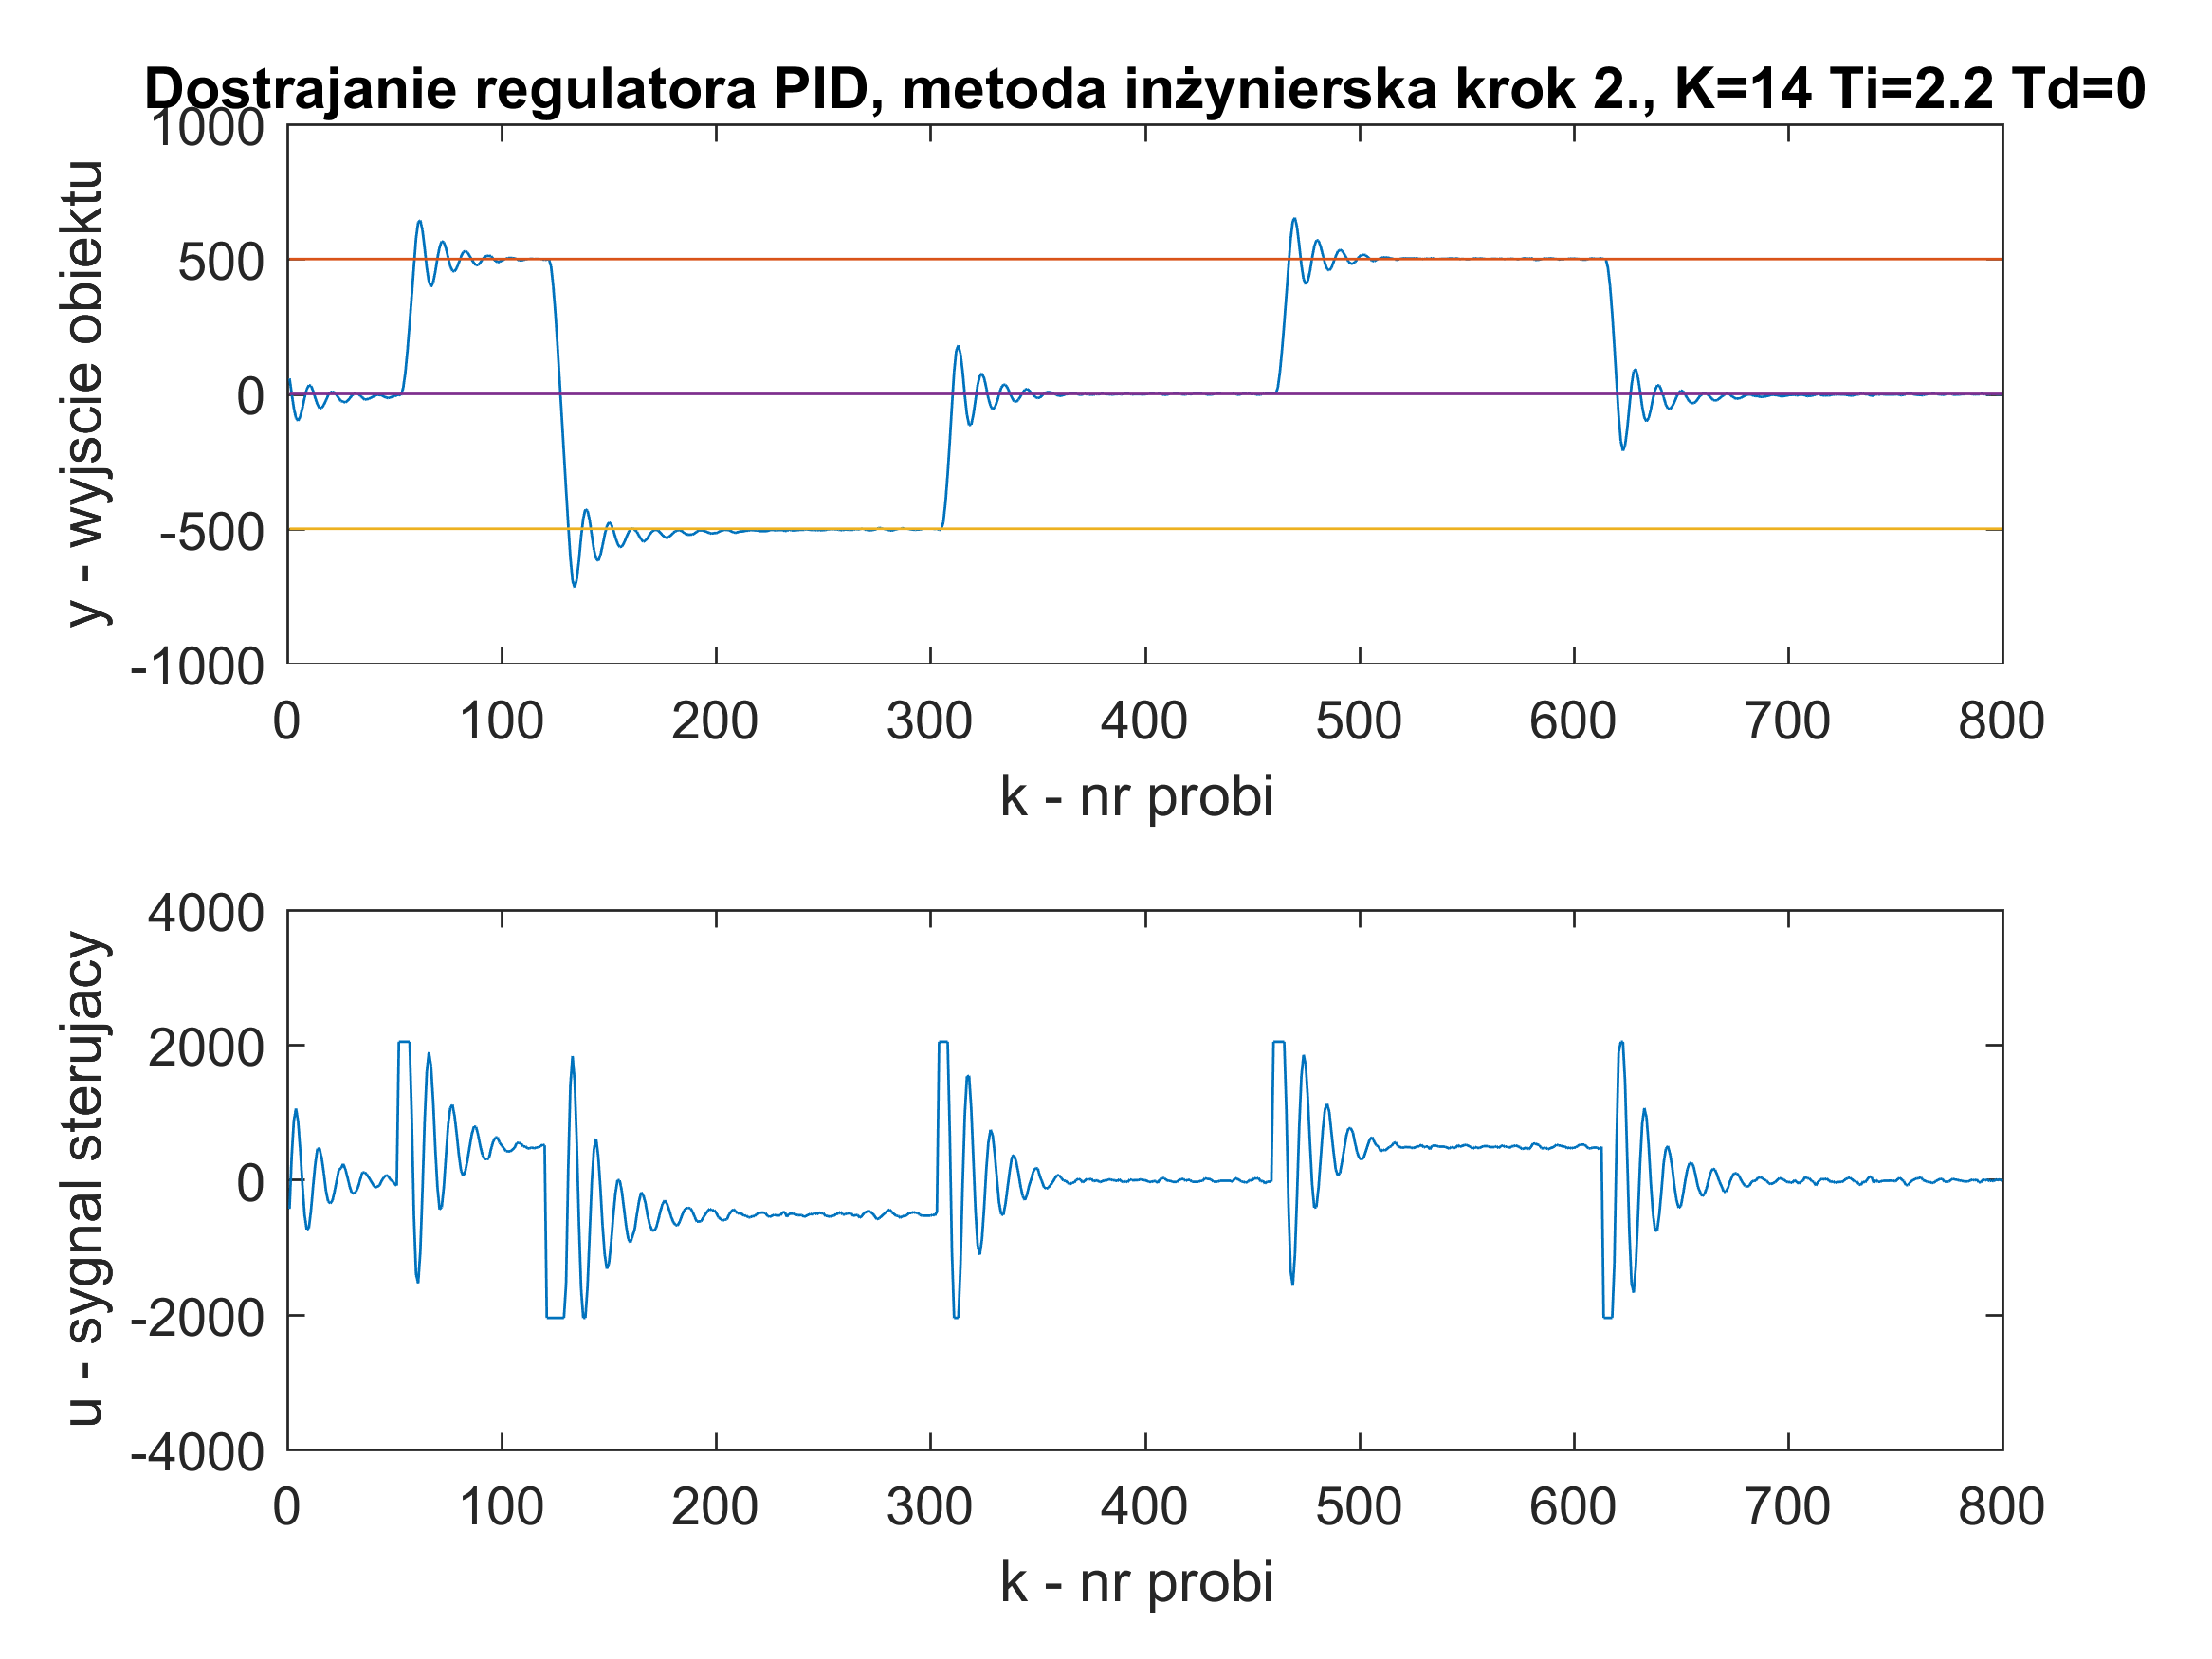
\includegraphics[width=0.9\linewidth]{MI_ti2200}
	\caption{Wyjście obiektu przy $T_{I}=2,2$ }
	\label{fig:MI_ti2200}
\end{figure}
\begin{figure}[H]
	\centering
	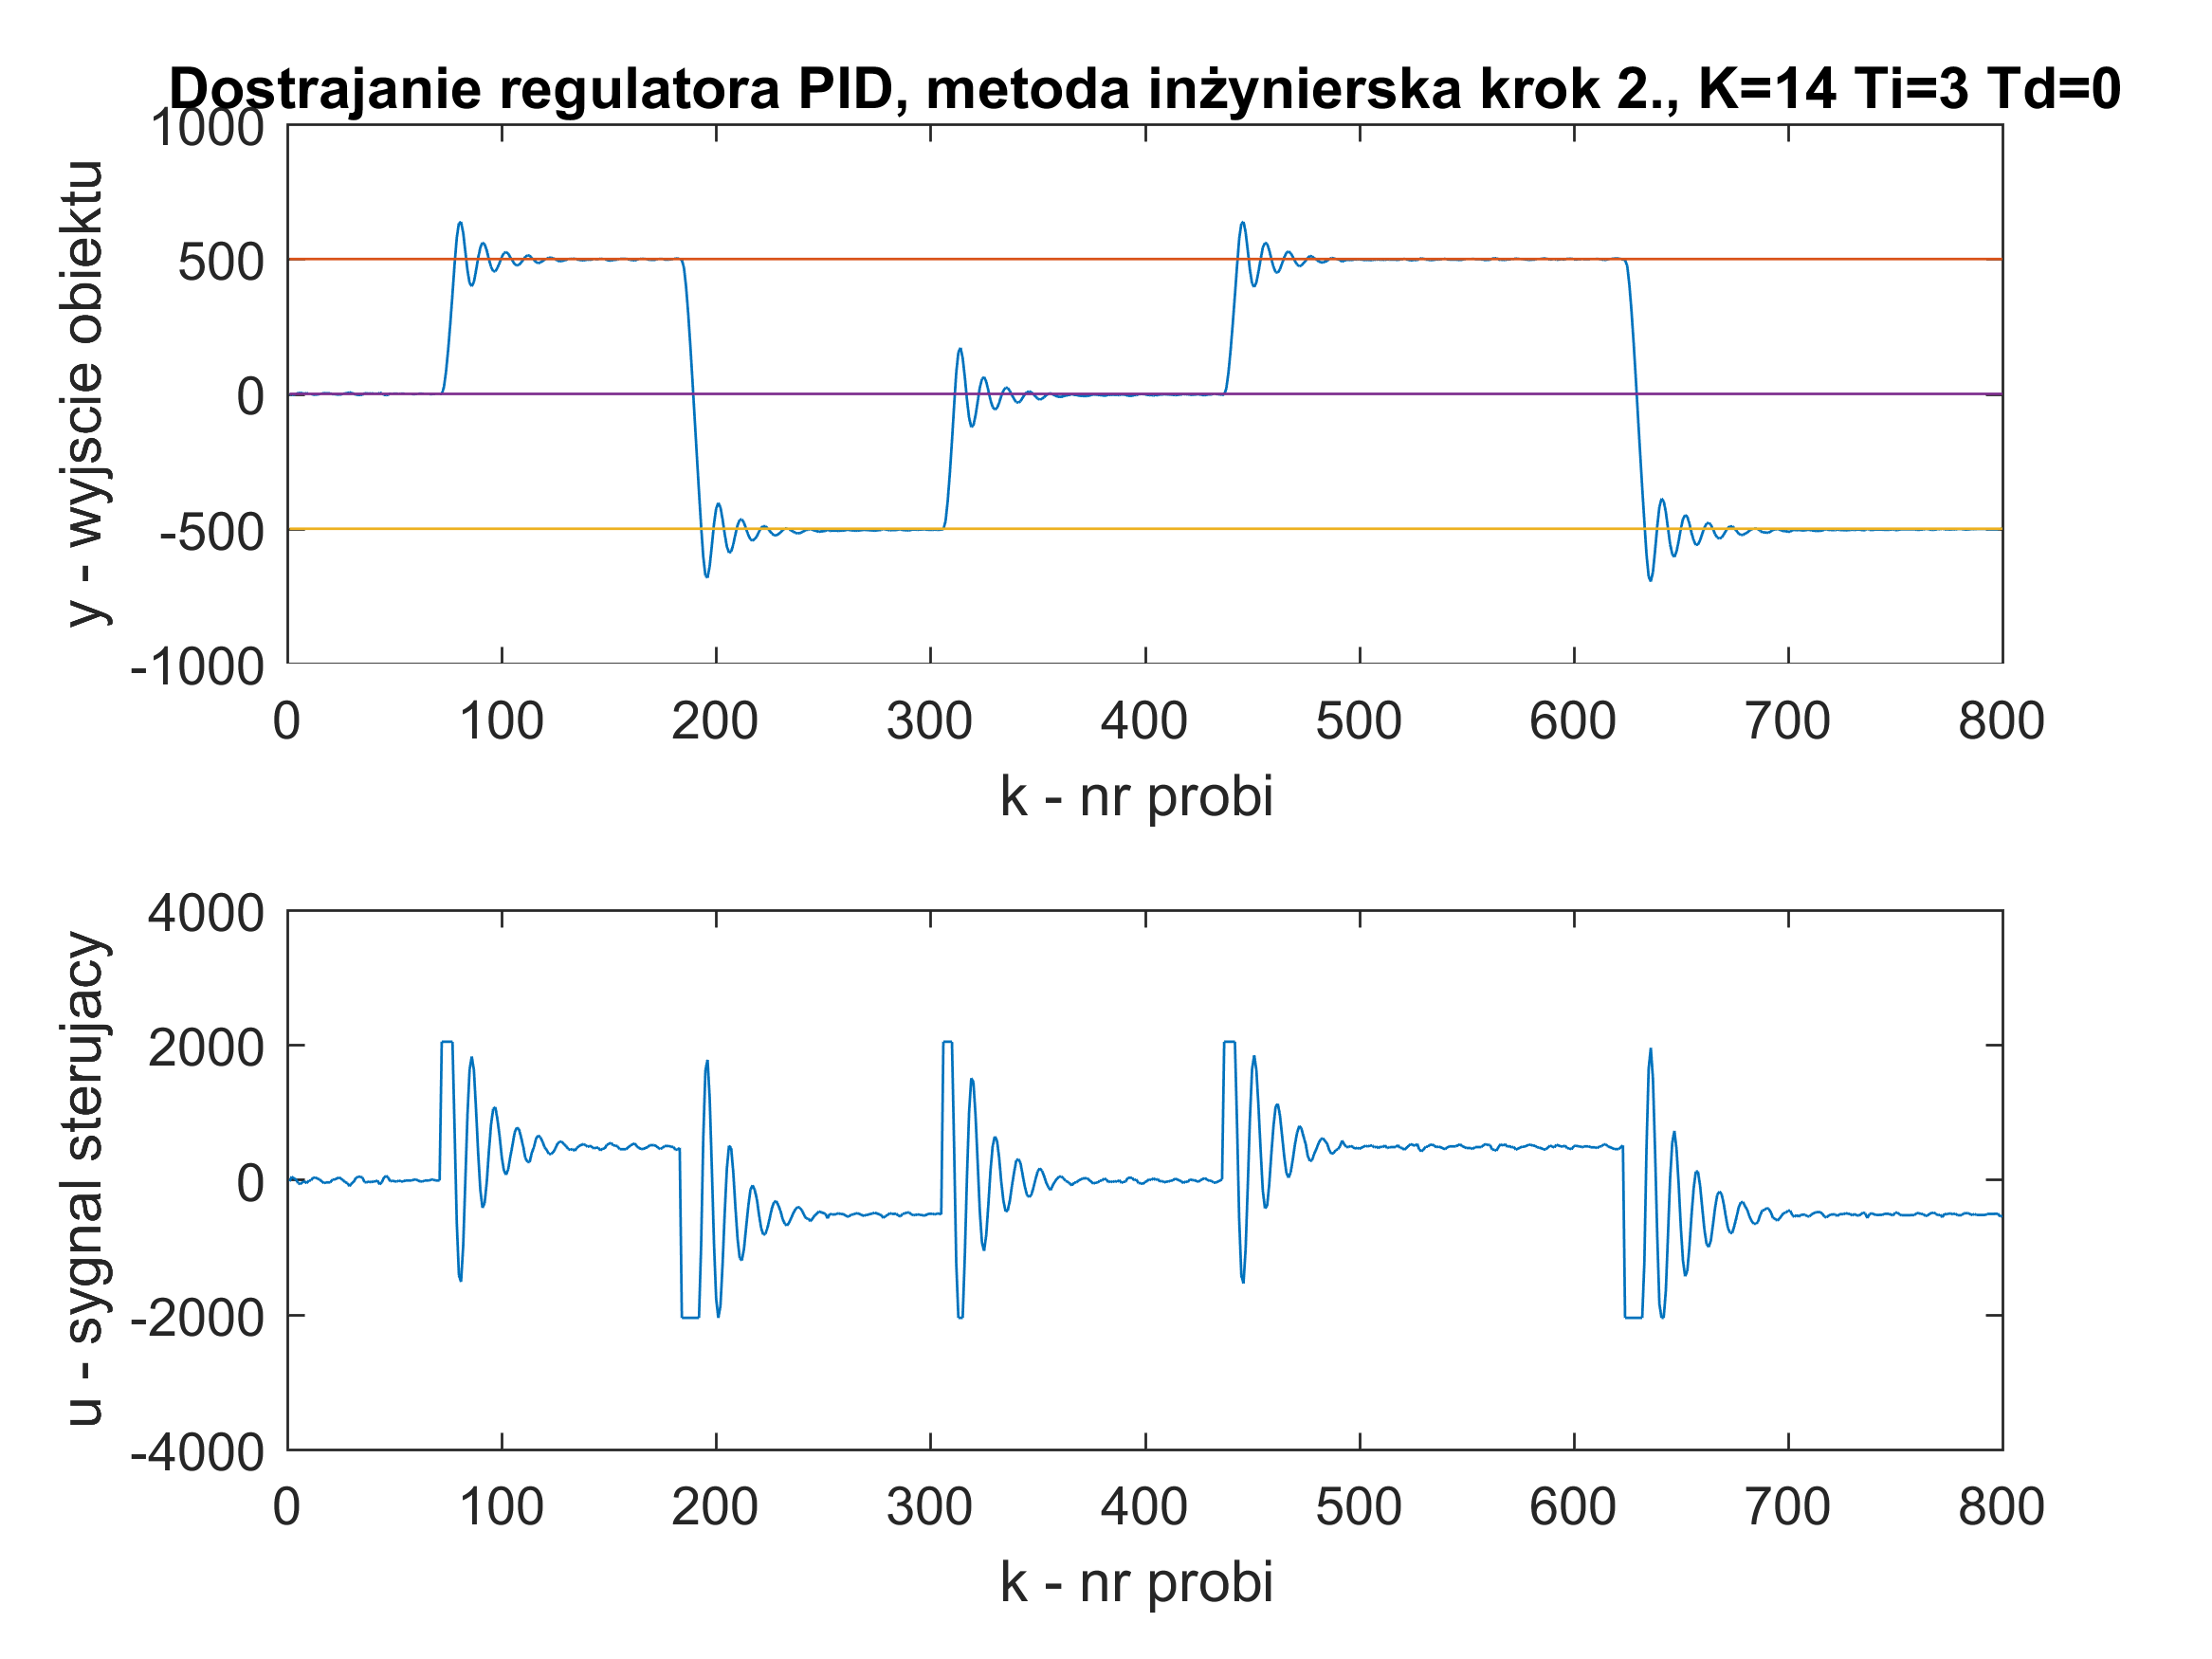
\includegraphics[width=0.9\linewidth]{MI_ti3000}
	\caption{Wyjście obiektu przy $T_{I}=3,0$ }
	\label{fig:MI_ti3000}
\end{figure}
\begin{figure}[H]
	\centering
	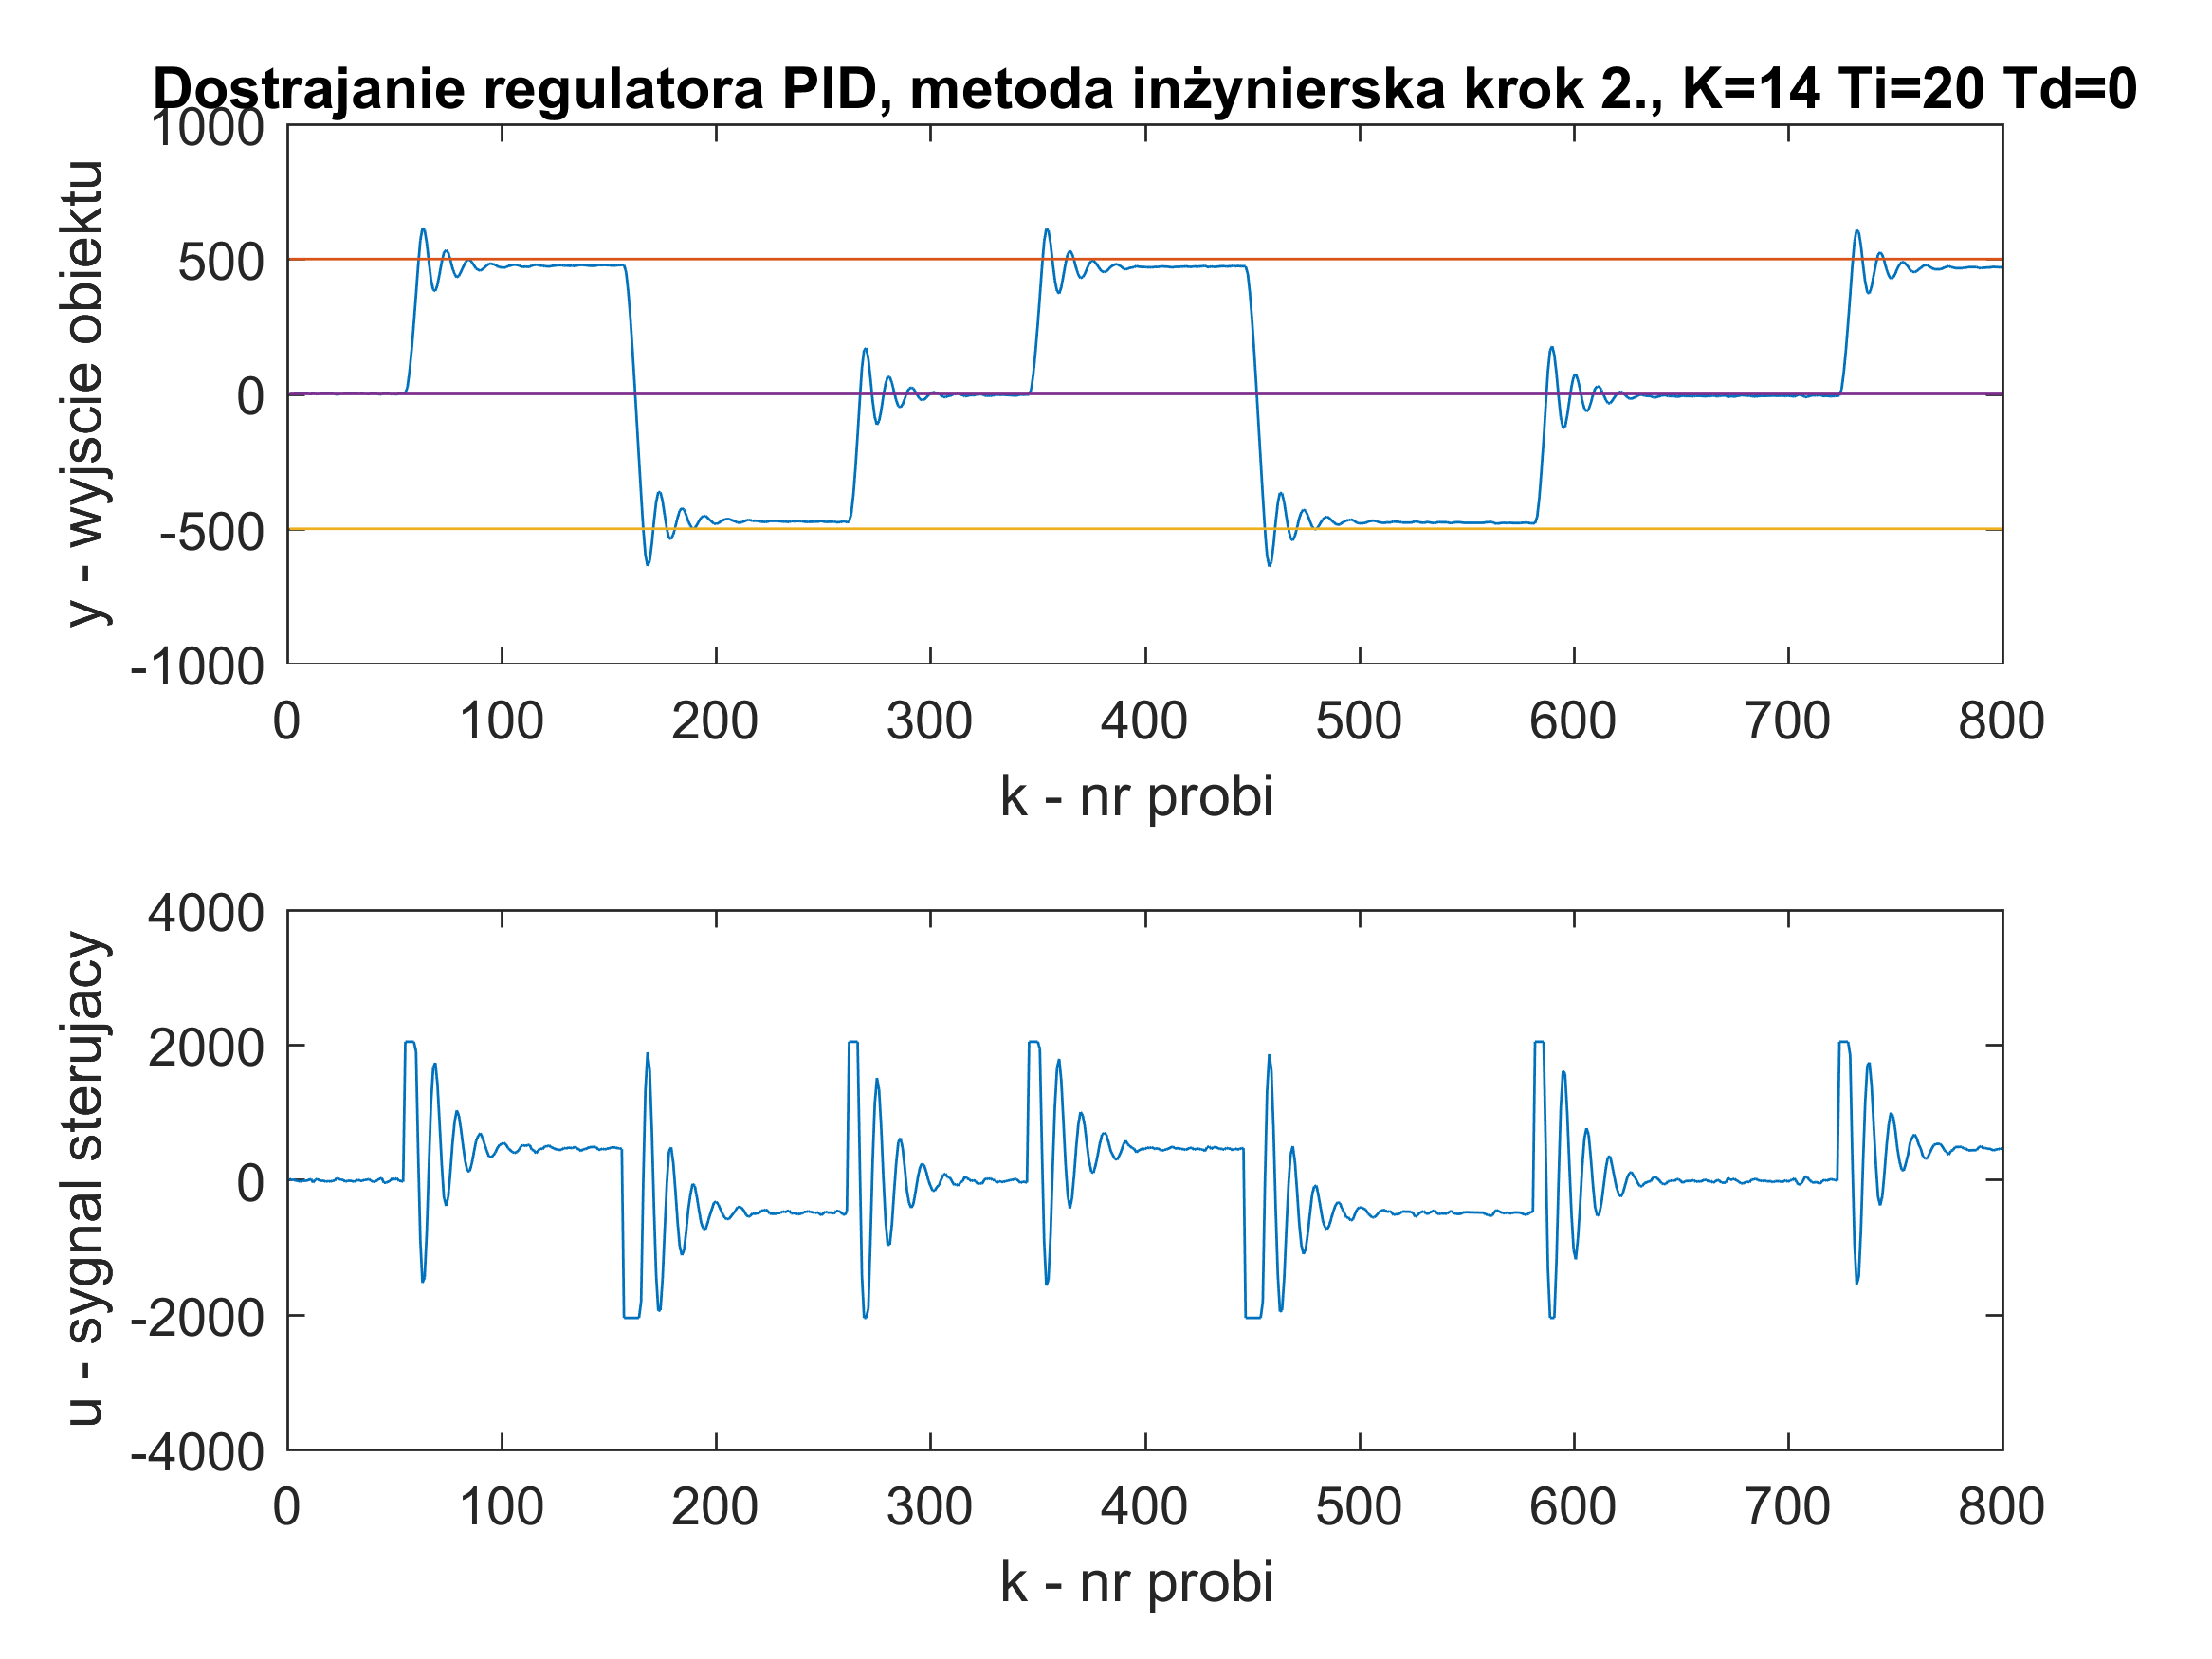
\includegraphics[width=0.9\linewidth]{MI_ti20000}
	\caption{Wyjście obiektu przy $T_{I}=20,0$ }
	\label{fig:MI_ti20000}
\end{figure}

Na wykresie \ref{fig:MI_ti200} można zauważyć, że zbyt mały czas zdwojenia, a tym samym zbyt duże znaczenie całkowania w wyznaczaniu sterowania, wprowadza oscylacje. Obiekt był stabilny tylko dzięki ograniczeniom na wartości sygnału sterującego. Z tego powodu przy drugim eksperymencie zwiększyłyśmy czas zdwojenia o jeden rząd wielkości. Przyjmując $T_{I}=2,0$ udało się osiągnąć zerowy uchyb ustalony oraz stosunkowo niewielkie przeregulowanie, które będziemy w stanie wyeliminować dołączając człon różniczkujący. Przy $T_{I}=20,0$, jak można zauważyć na rysunku \ref{fig:MI_ti20000}, układ wolniej się stabilizował - przez dłuższy czas występował niezerowy uchyb. Zmiana wartości czasu zdwojenia w okolicach $T_{I}=2,0$ nie powodowała zauważalnej różnicy w jakości regulacji. W wyniku przeprowadzonych eksperymentów przyjęłyśmy $T_{I}=2,0$.

\subsubsection{Krok 3. - Dobór parametru $T_{D}$}

Przy doborze parametru $T_{D}$ korzysta się z pełnego regulatora PID, czyli:\\
\[u(k)=u_{P}(k)+u_{I}(k)+ u_{D}(k)\]
Zgodnie z poprzednimi krokami przyjęte zostało $K=14$, $T_{I}=2,0$.
Przeprowadzone zostały eksperymenty dla $T_{D}$ równego kolejno: $T_{D}=0,5$ , $T_{D}=0,1$ , $T_{D}=0,08$ , $T_{D}=0,05$.

\begin{figure}[H]
	\centering
	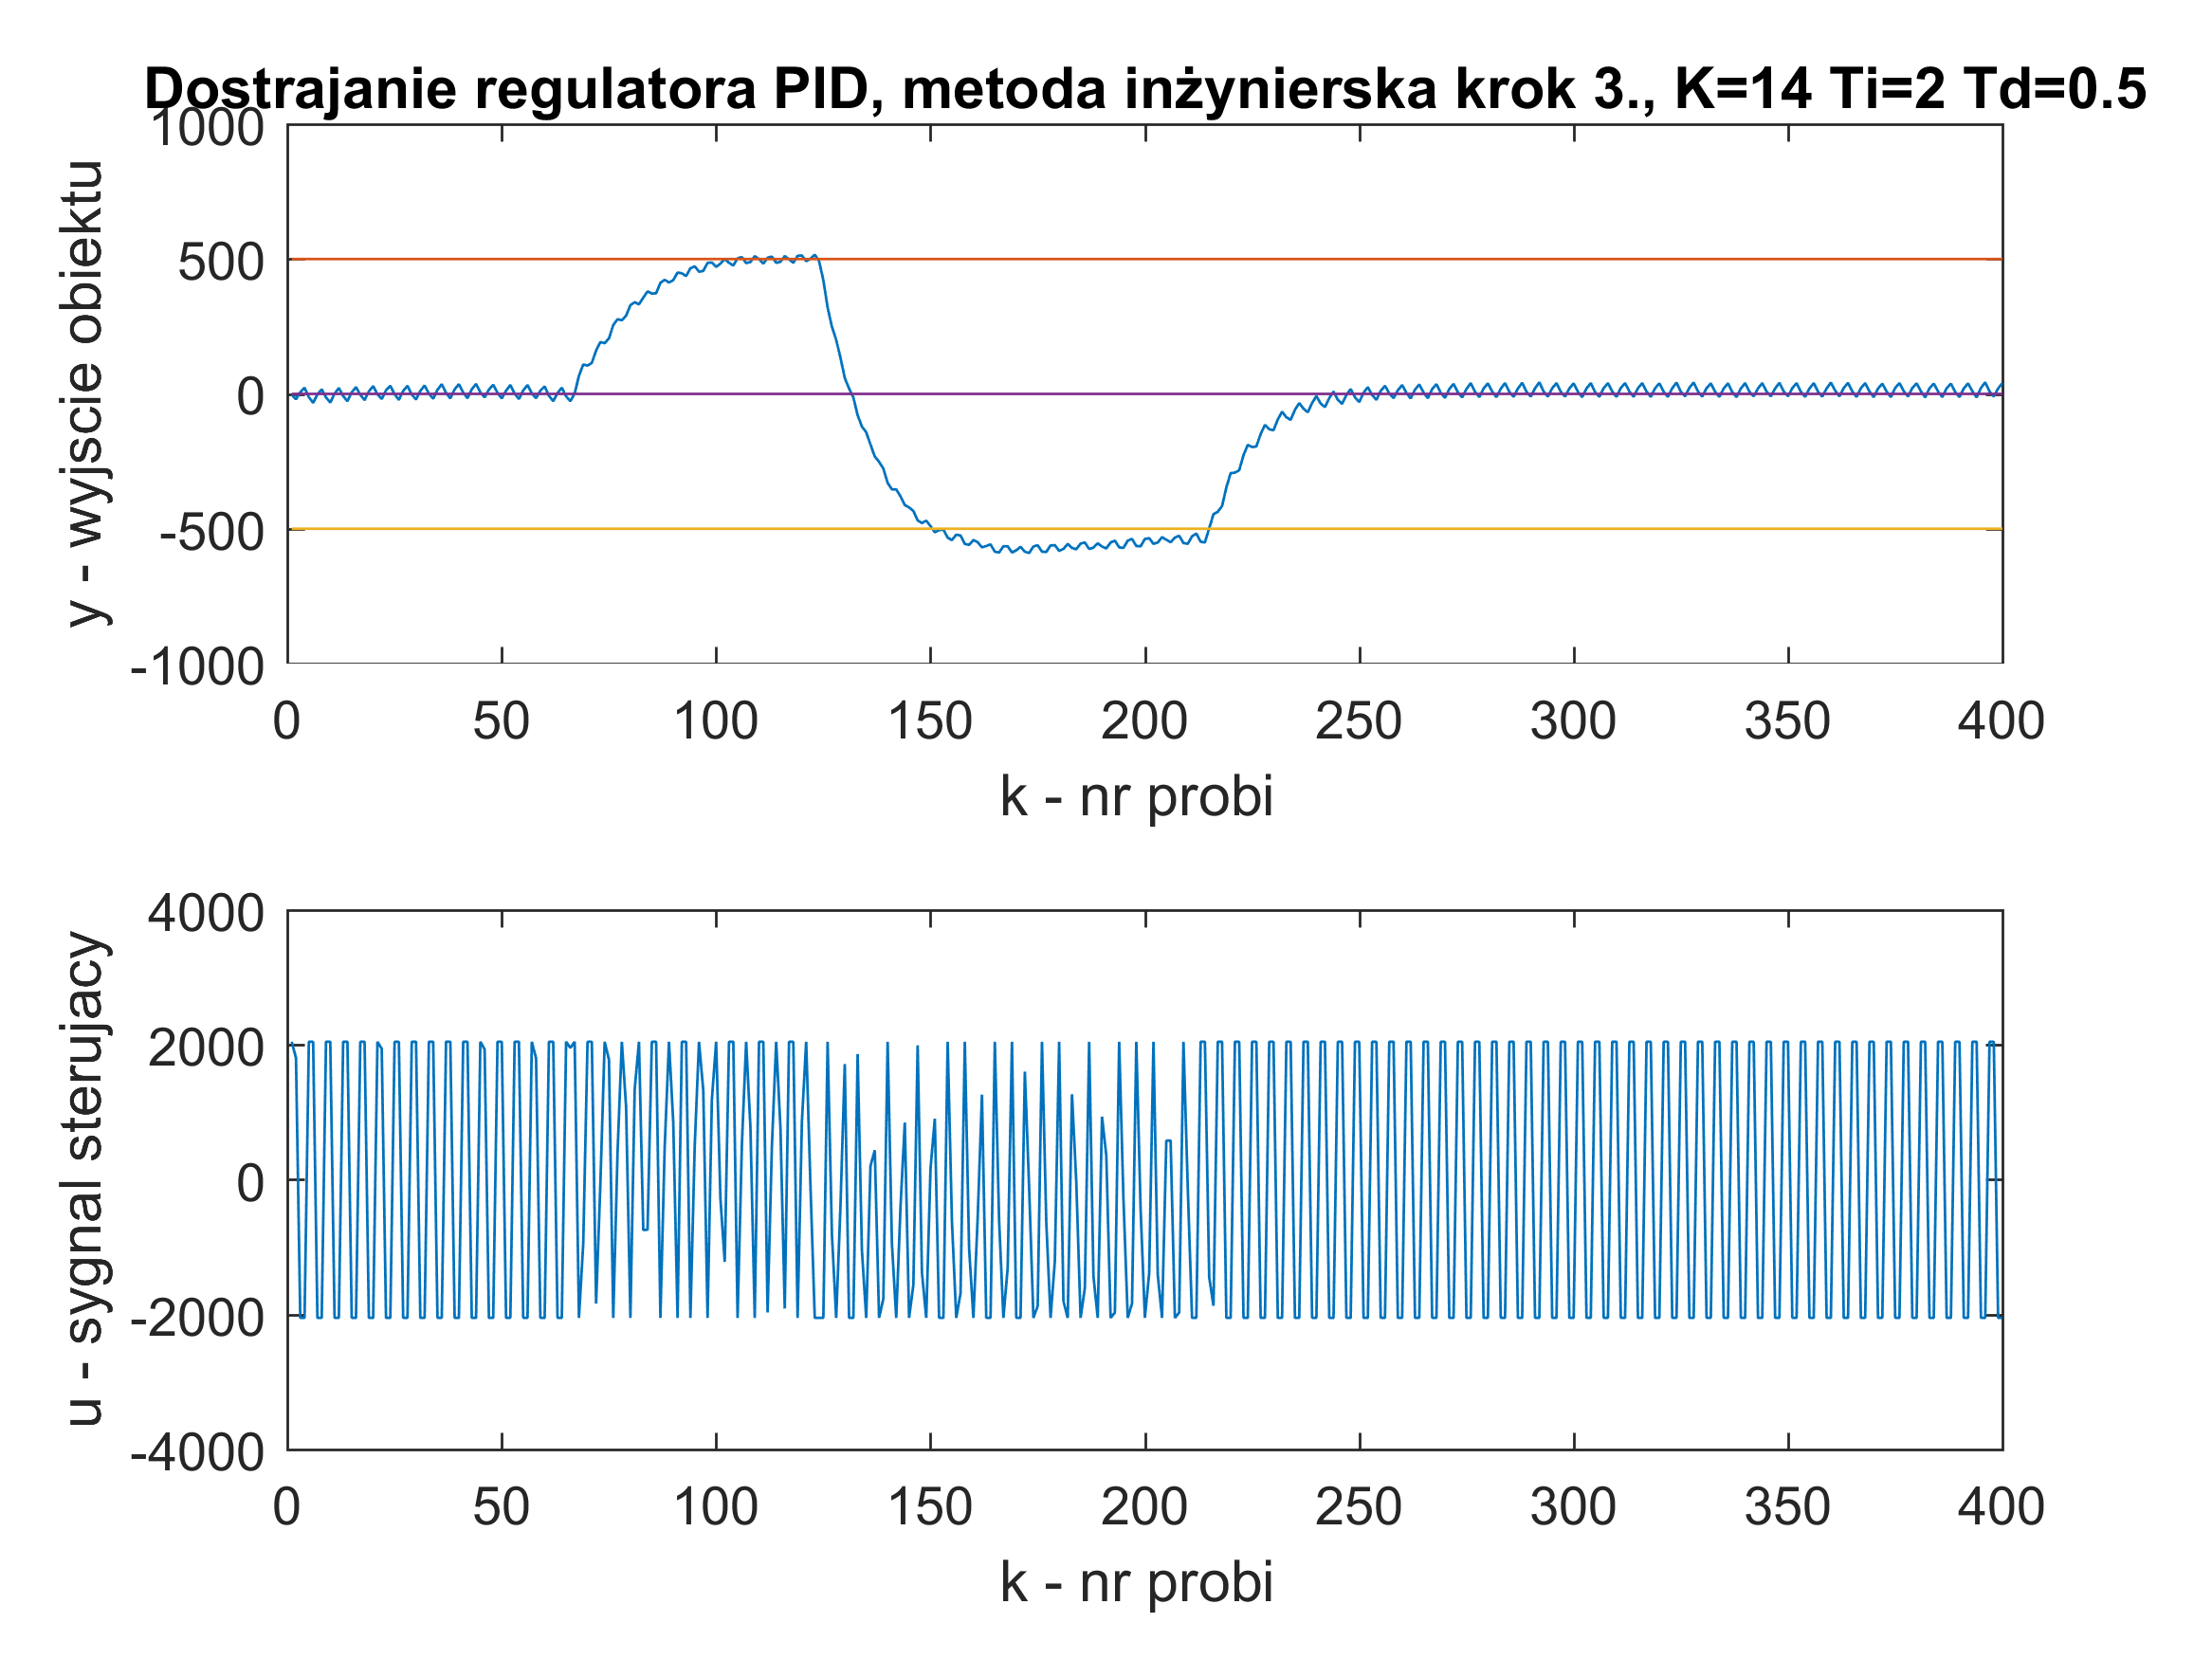
\includegraphics[width=0.9\linewidth]{MI_td500}
	\caption{Wyjście obiektu przy $T_{D}=0,5$ }
	\label{fig:MI_td500}
\end{figure}
\begin{figure}[H]
	\centering
	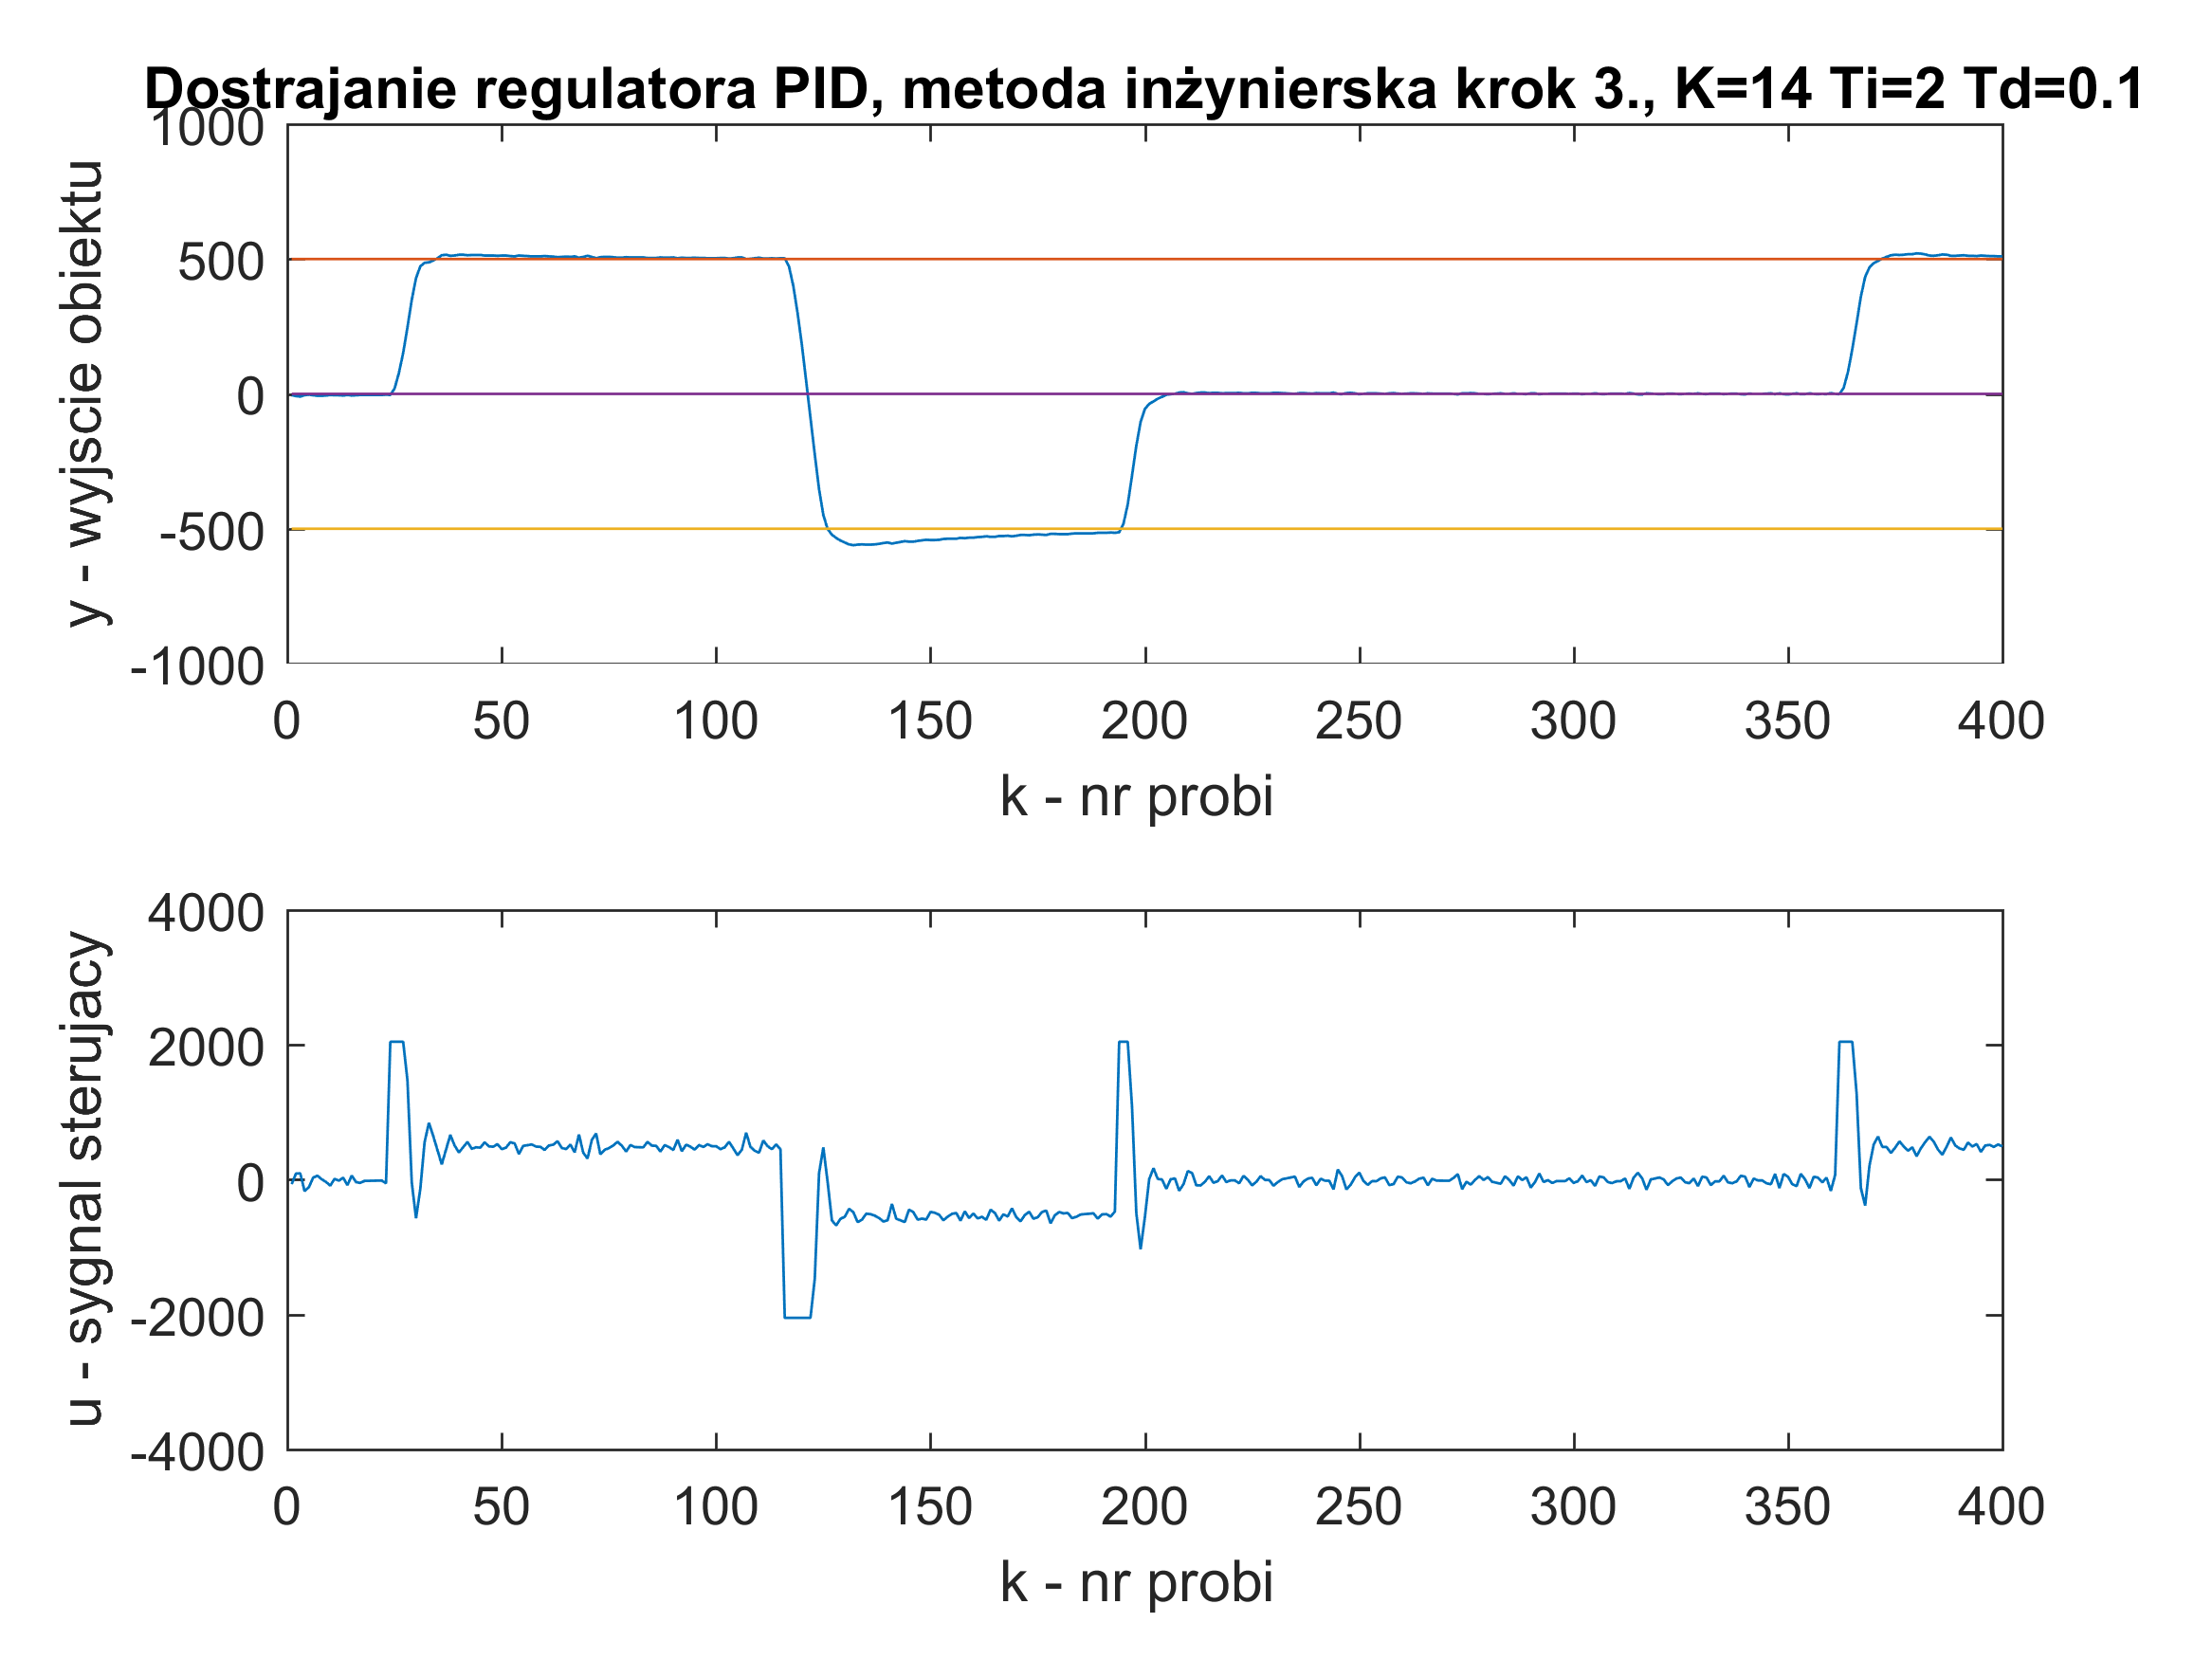
\includegraphics[width=0.9\linewidth]{MI_td100}
	\caption{Wyjście obiektu przy $T_{D}=0,1$ }
	\label{fig:MI_td100}
\end{figure}
\begin{figure}[H]
	\centering
	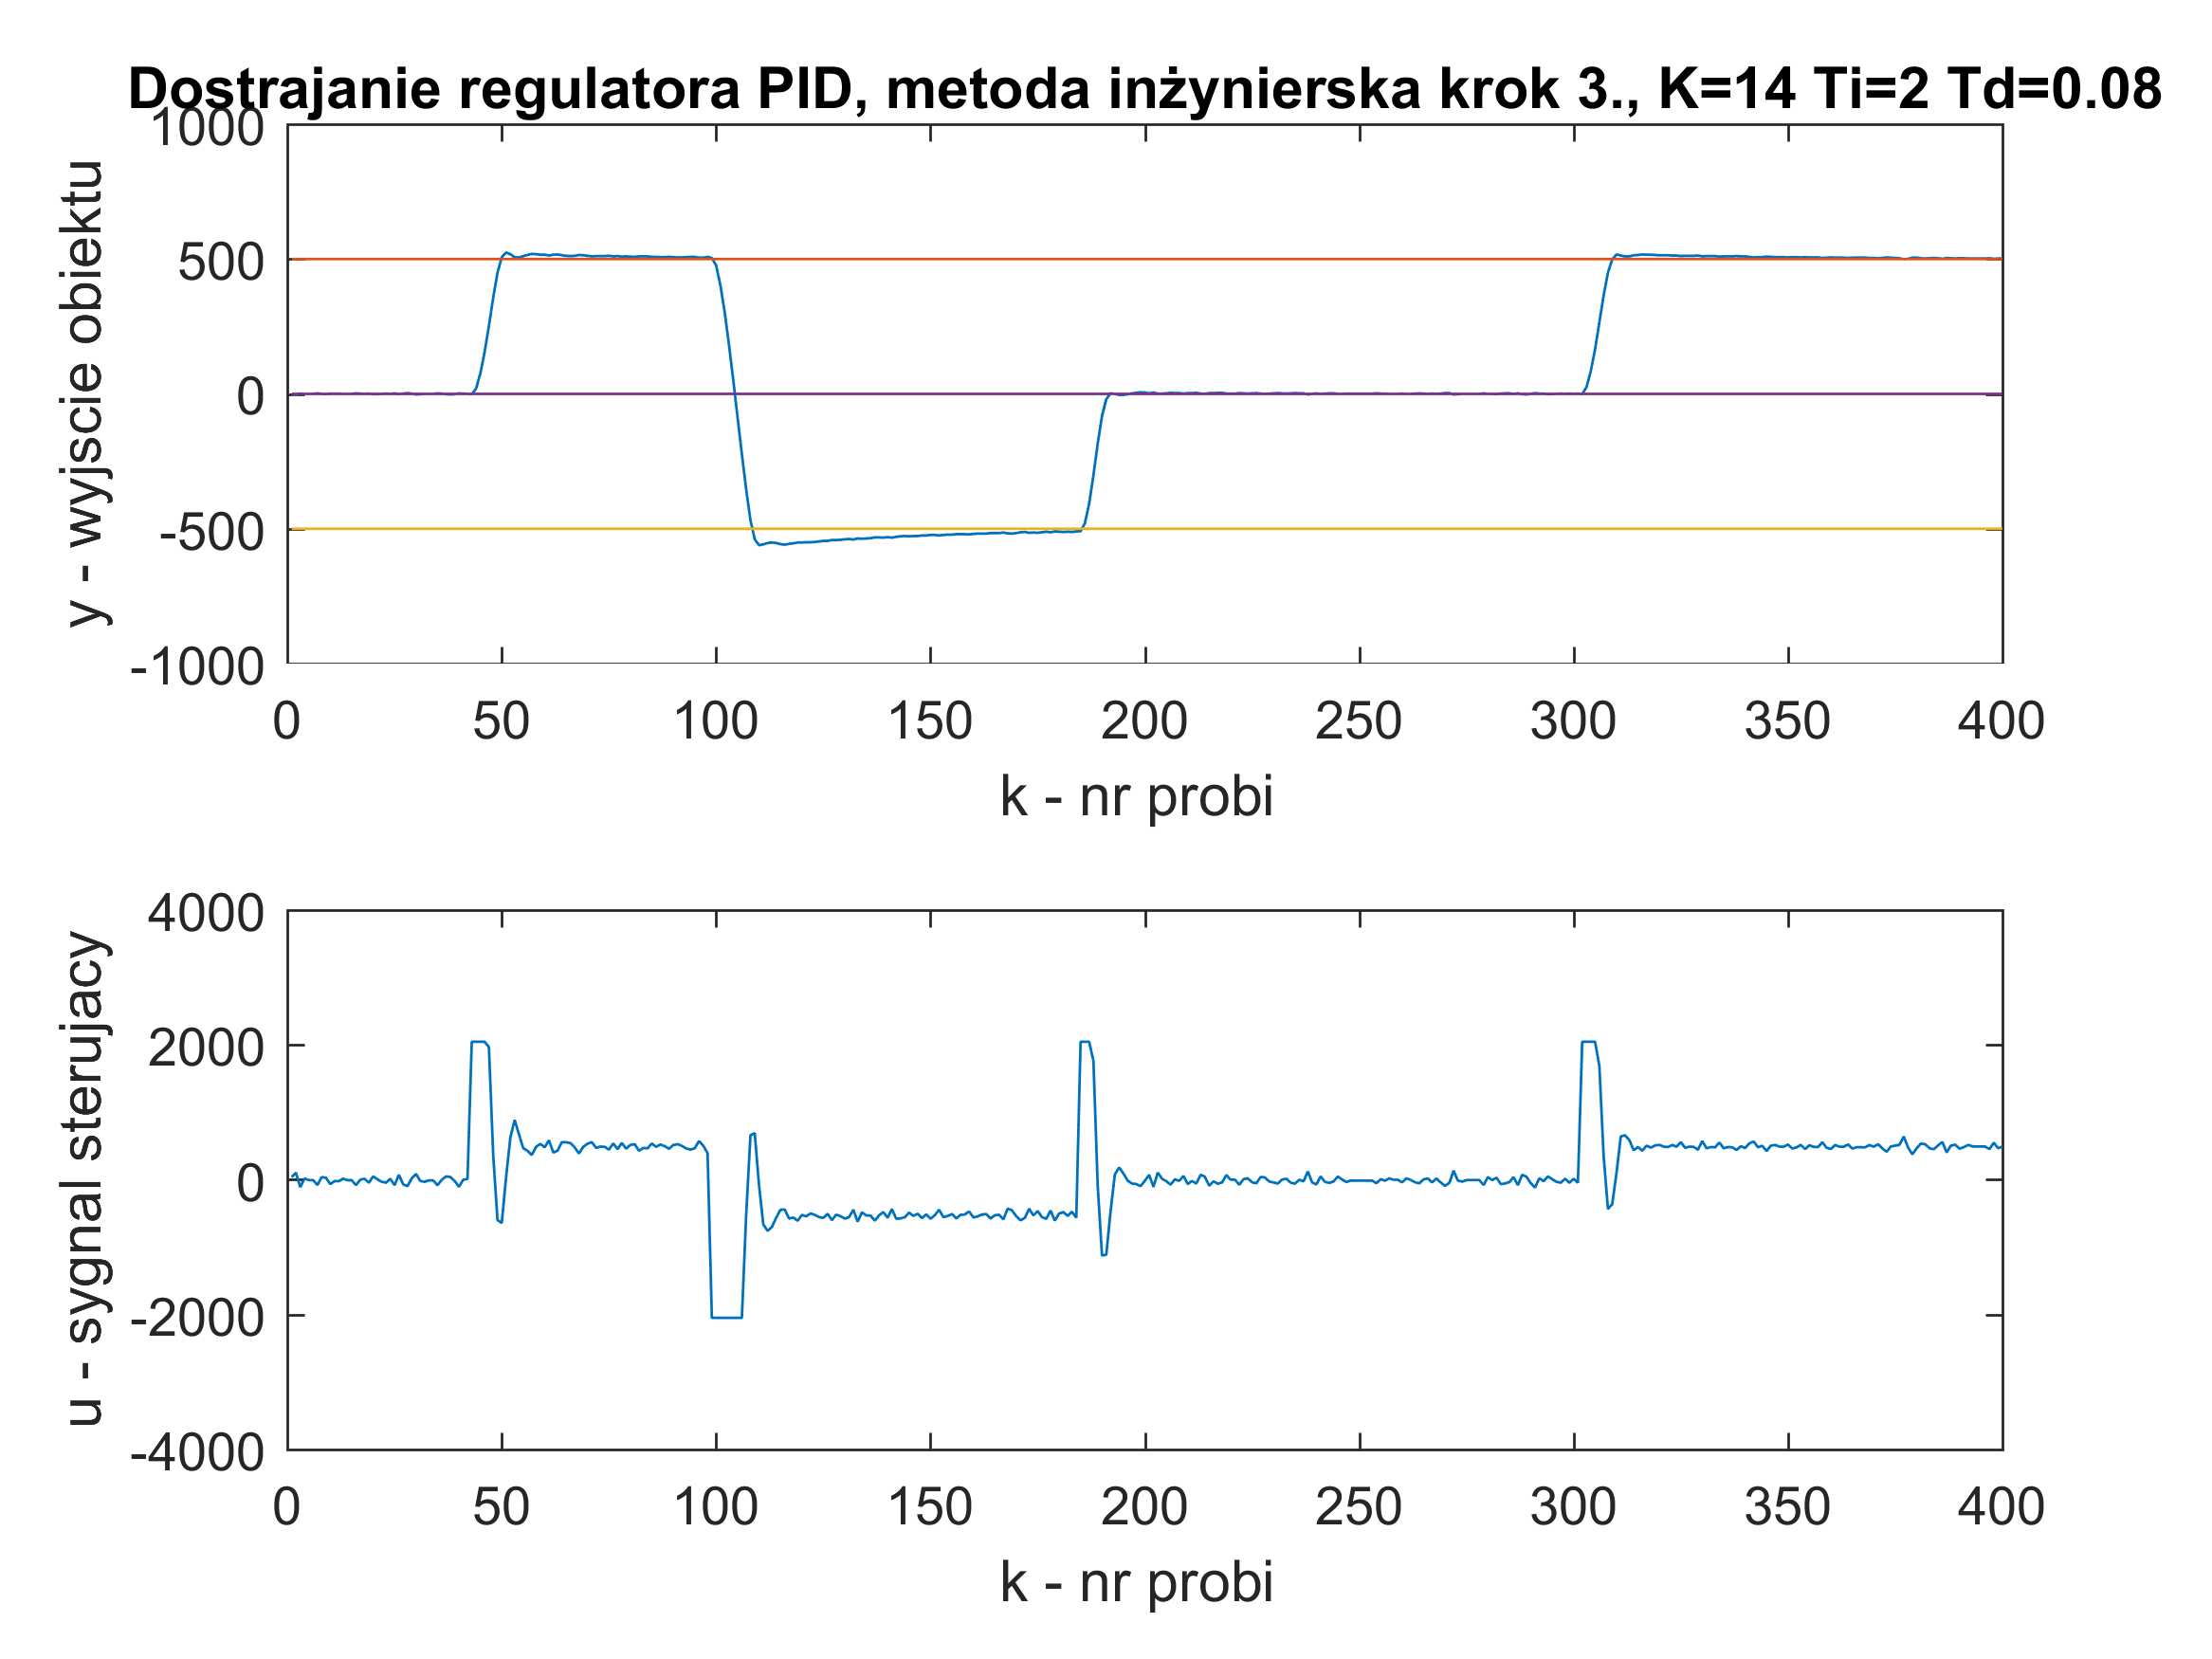
\includegraphics[width=0.9\linewidth]{MI_td80}
	\caption{Wyjście obiektu przy $T_{D}=0,08$ }
	\label{fig:MI_td80}
\end{figure}
\begin{figure}[H]
	\centering
	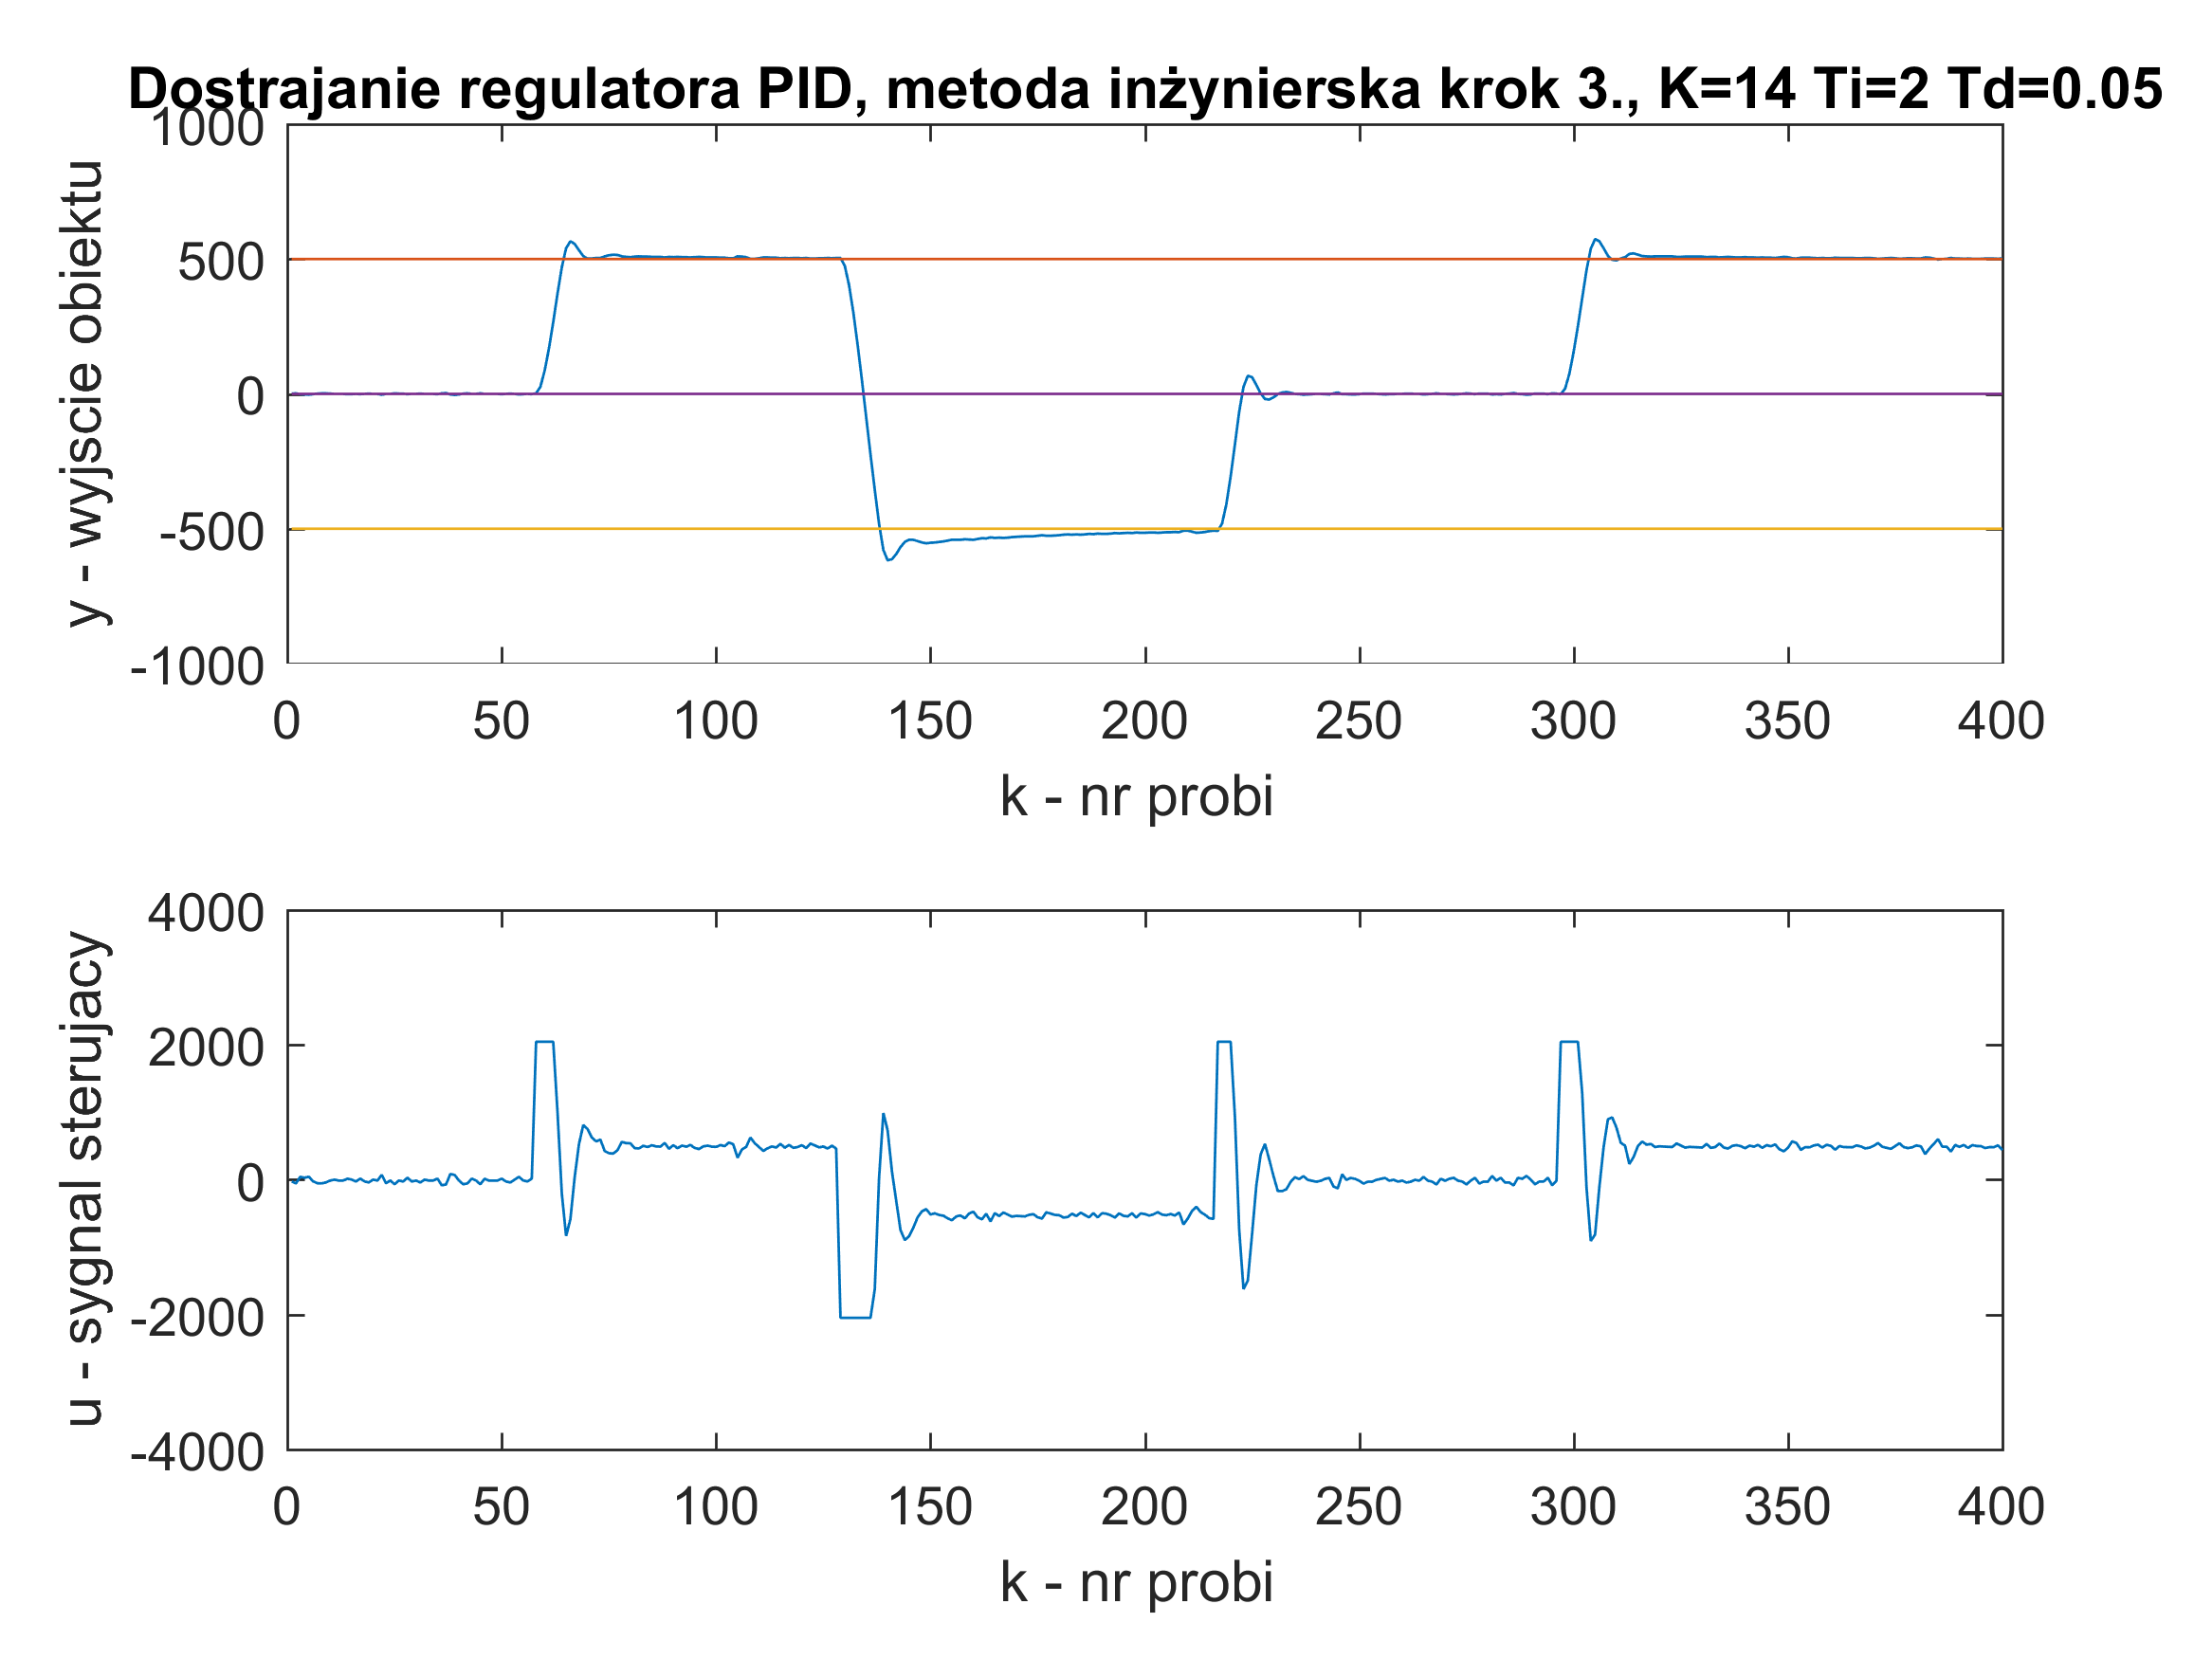
\includegraphics[width=0.9\linewidth]{MI_td50}
	\caption{Wyjście obiektu przy $T_{D}=0,05$ }
	\label{fig:MI_td50}
\end{figure}

Na wykresie \ref{fig:MI_td500} można zauważyć, że przy stosunkowo dużym czasie wyprzedzenia obiekt wolno osiąga zadaną wartość, a przebieg sygnału sterującego odbija się od ograniczeń. Z wykresu \ref{fig:MI_td100} wynika, że zmniejszenie 5. razy parametru $T_{D}$ powoduje ograniczenie zmienności sygnału sterującego, a co za tym idzie ustabilizowanie się wyjścia obiektu. Występuje niewielkie przeregulowanie spowodowane obliczeniem sterowania wykraczającego poza ograniczenia. Zmniejszenie $T_{D}$ do $T_{D}=0,05$ powoduje zwiększenie przeregulowania - jest zbyt mały wpływ członu różniczkującego. Przy ustawieniu czasu wyprzedzenia równym $T_{D}=0,08$ osiągamy niegorsze rezultaty, jak przy $T_{D}=0,1$. Z tego powodu ustaliłyśmy następujące parametry regulatora PID:
\[K=14,   T_{I}=2,0,   T_{D}=0,08.\]

\subsubsection{Krok 4. - Dostrojenie regulatora}
Ostatni krok metody inżynierskiej polega na dostrojeniu regulatora. W tym celu dokonałyśmy kilka eksperymentów. Sprawdziłyśmy, czy da się polepszyć regulator modyfikując stałe $T_{I}$ i $K$.\\

1. Zwiększenie wpływu całki $K=14,  T_{I}=1,8,  T_{D}=0,08 $ 
\begin{figure}[H]
	\centering
	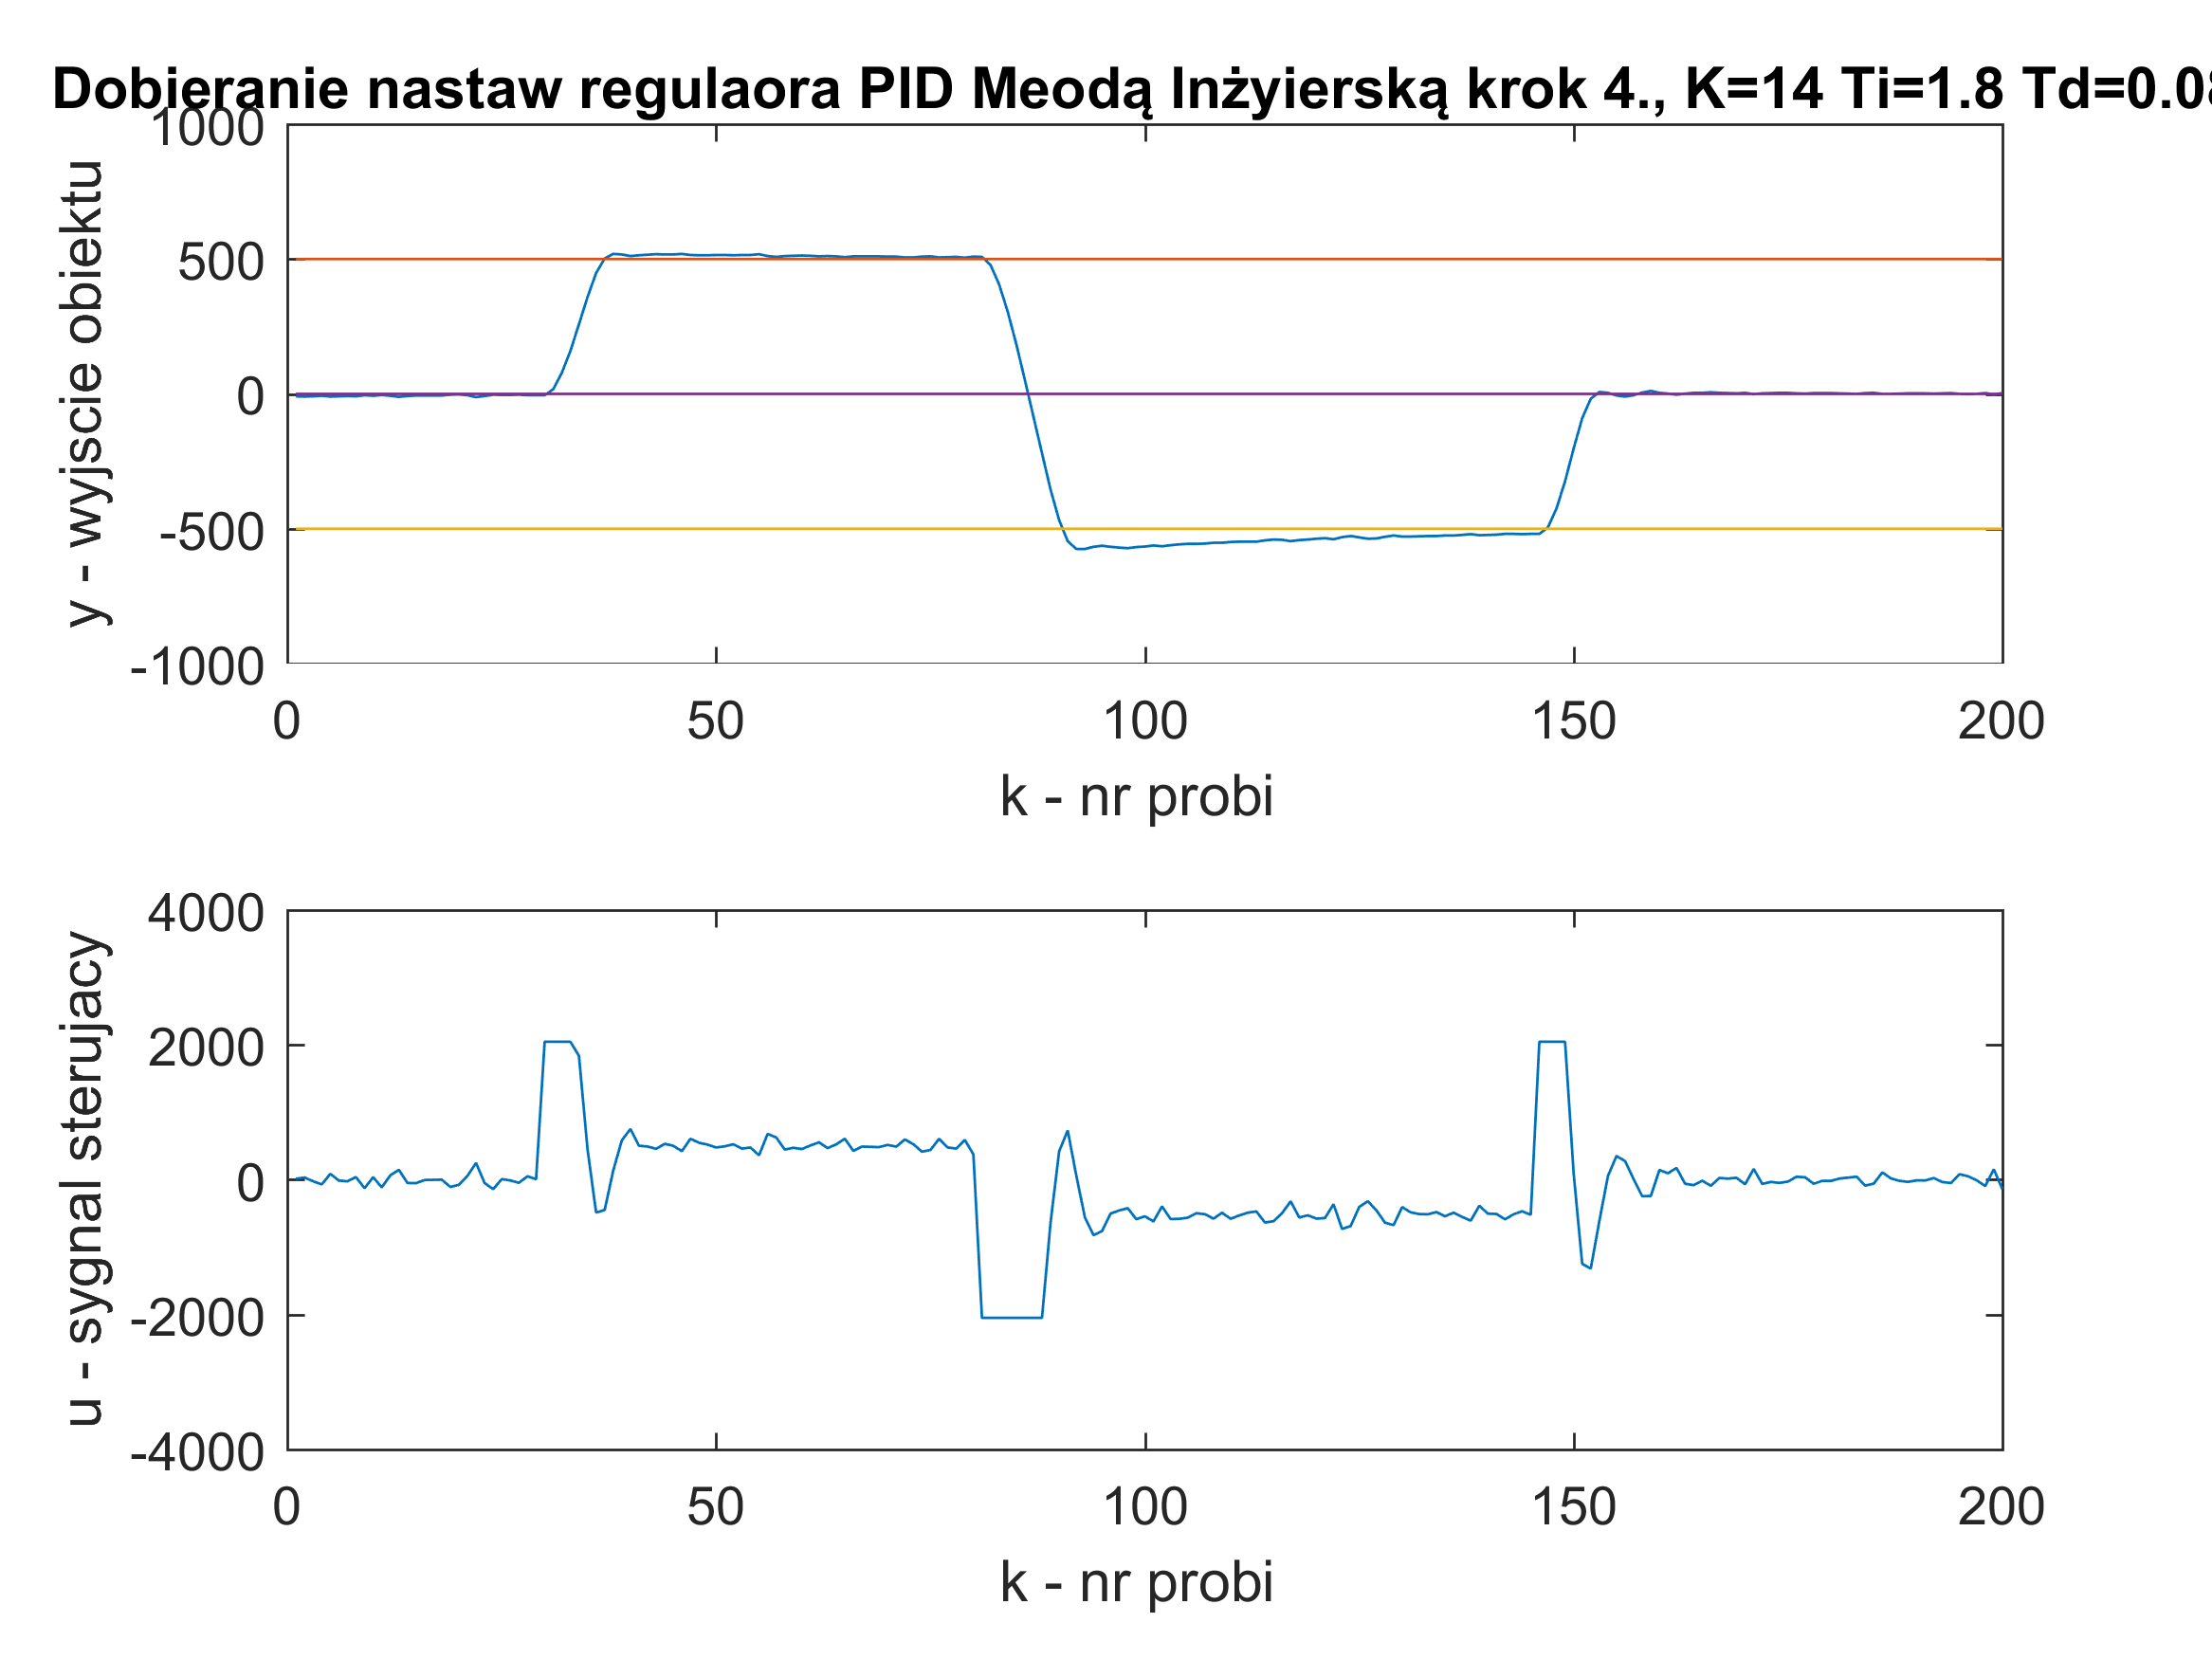
\includegraphics[width=0.9\linewidth]{MI_11}
	\caption{Wyjście obiektu przy $K=14, T_{I}=1,8, T_{D}=0,08 $  }
	\label{fig:MI_11}
\end{figure}
2. Zmniejszenie wpływu całki $K=14, T_{I}=2,2, T_{D}=0,08 $ 
\begin{figure}[H]
	\centering
	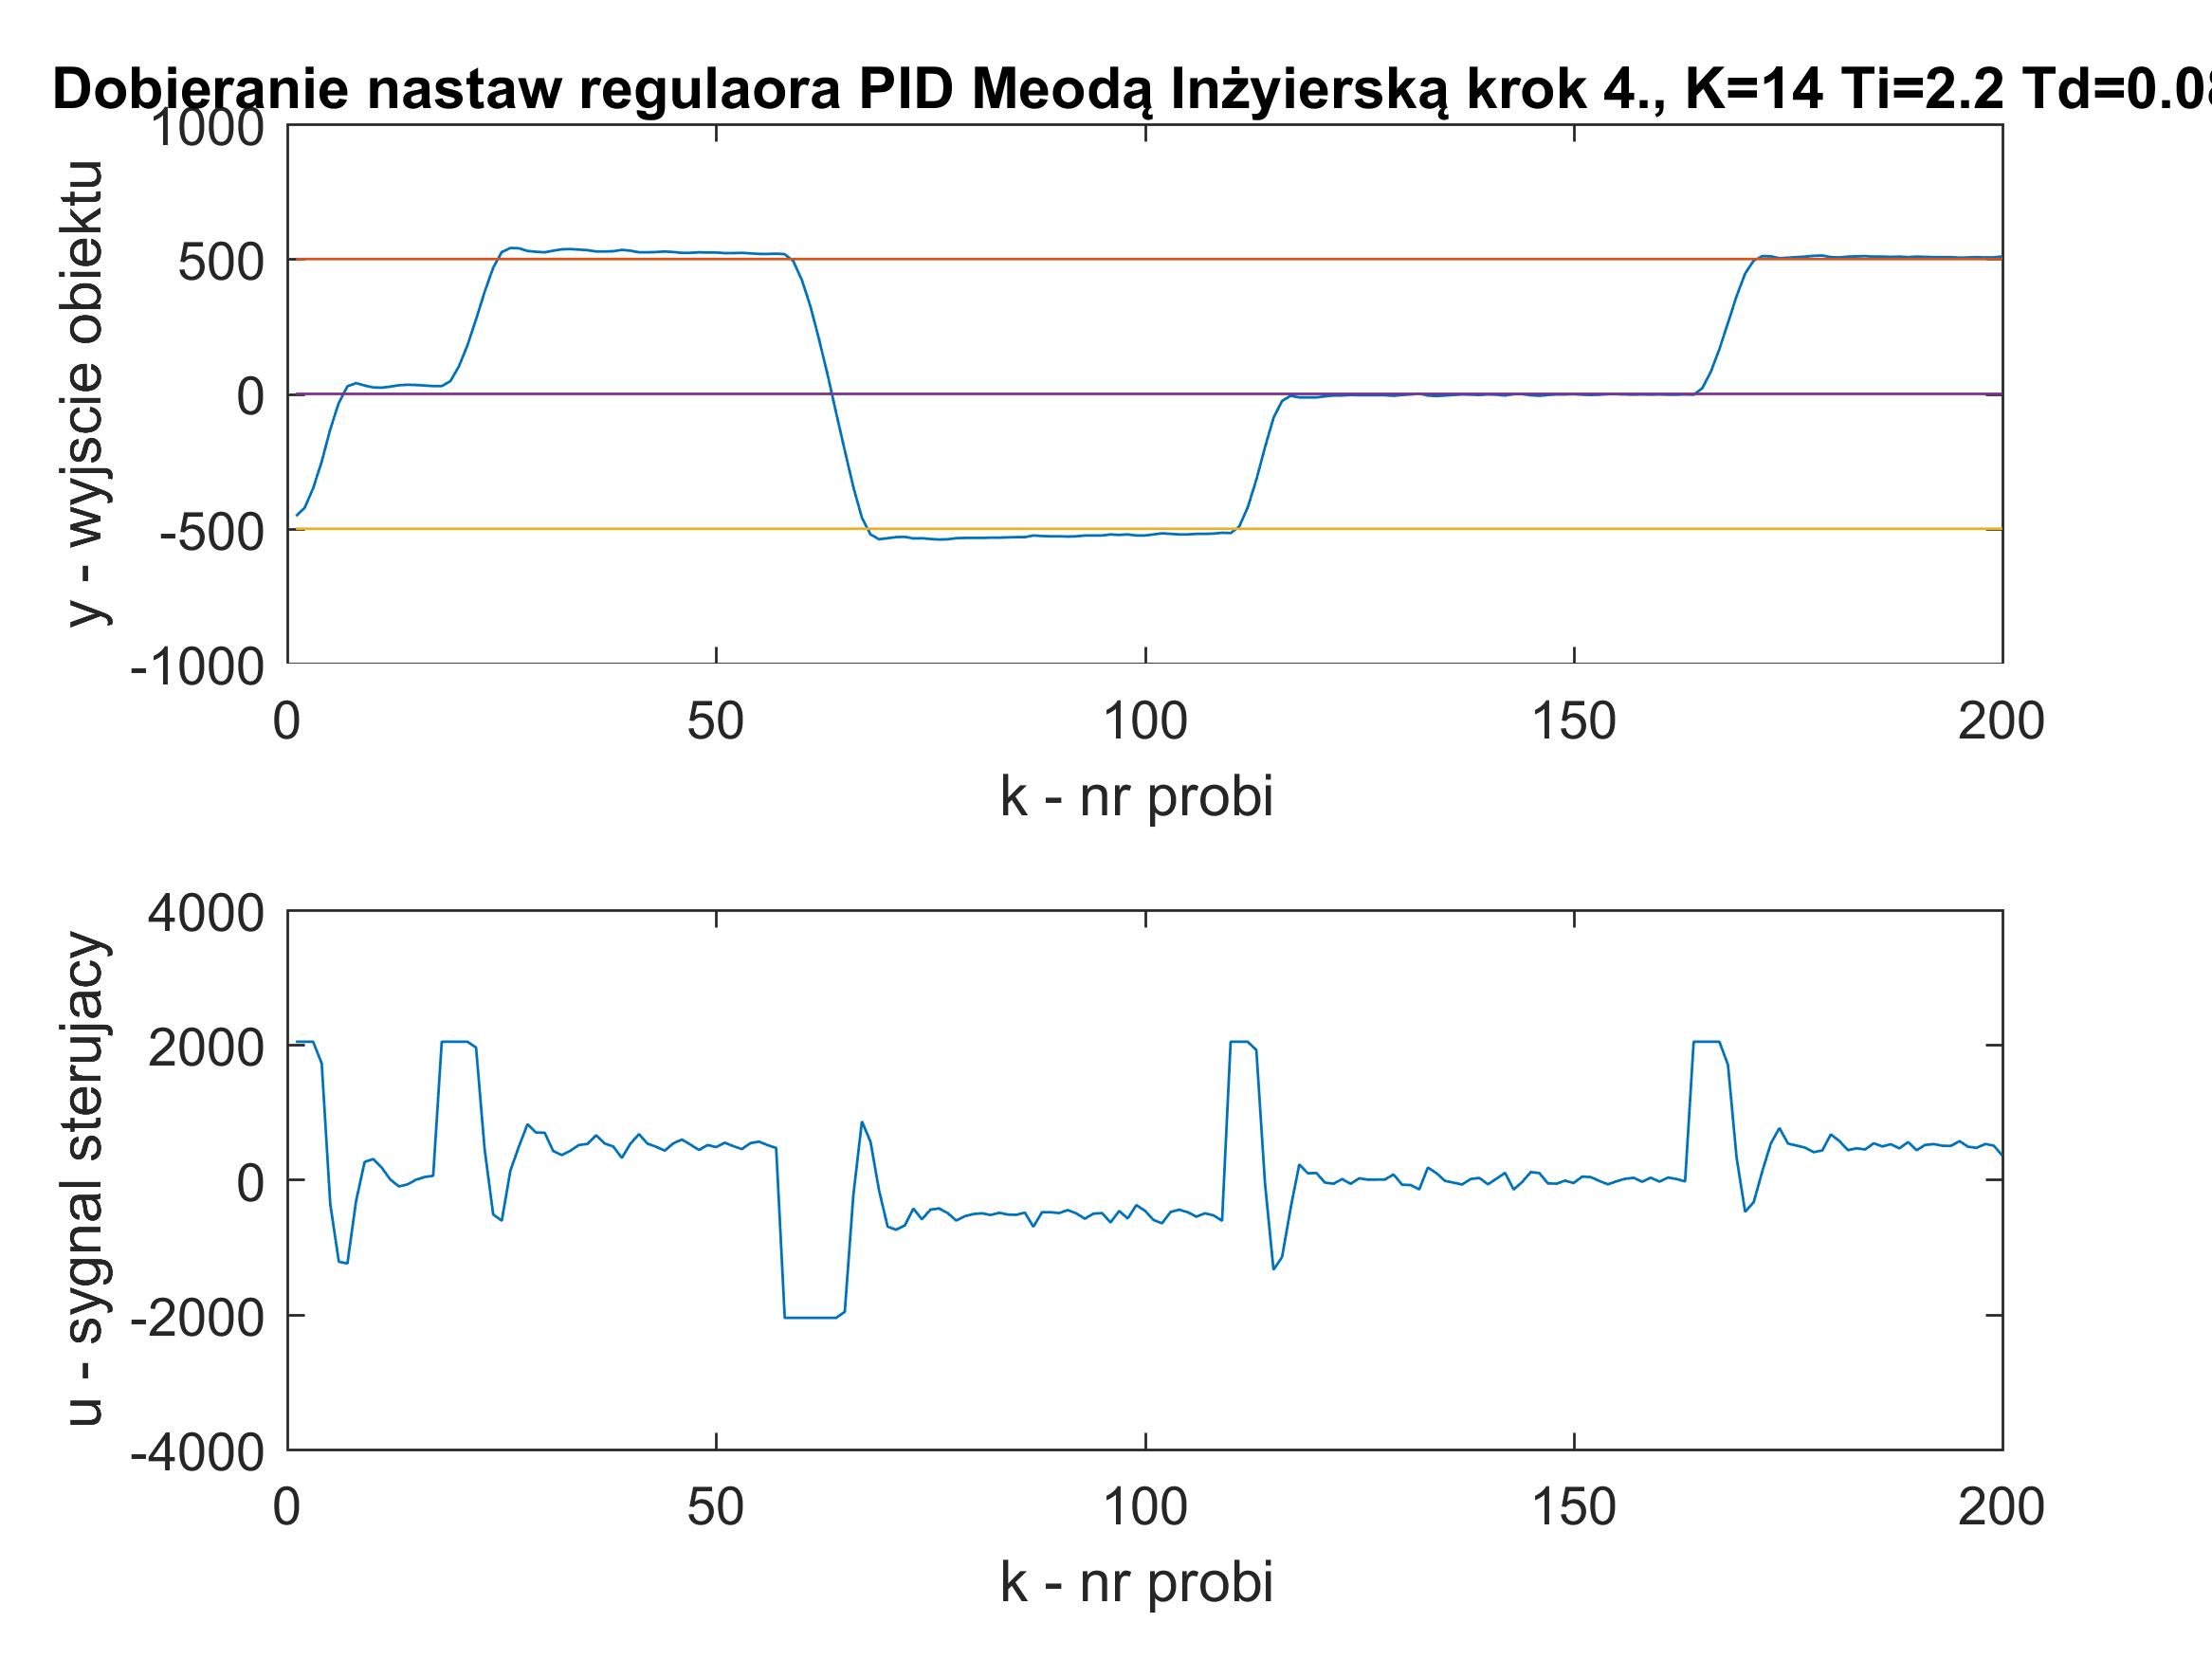
\includegraphics[width=0.9\linewidth]{MI_33}
	\caption{Wyjście obiektu przy $K=14, T_{I}=2,2, T_{D}=0,08 $  }
	\label{fig:MI_33}
\end{figure}
3. Zwiększenie wzmocnienia $K=15,  T_{I}=2,  T_{D}=0,08$ 
\begin{figure}[H]
	\centering
	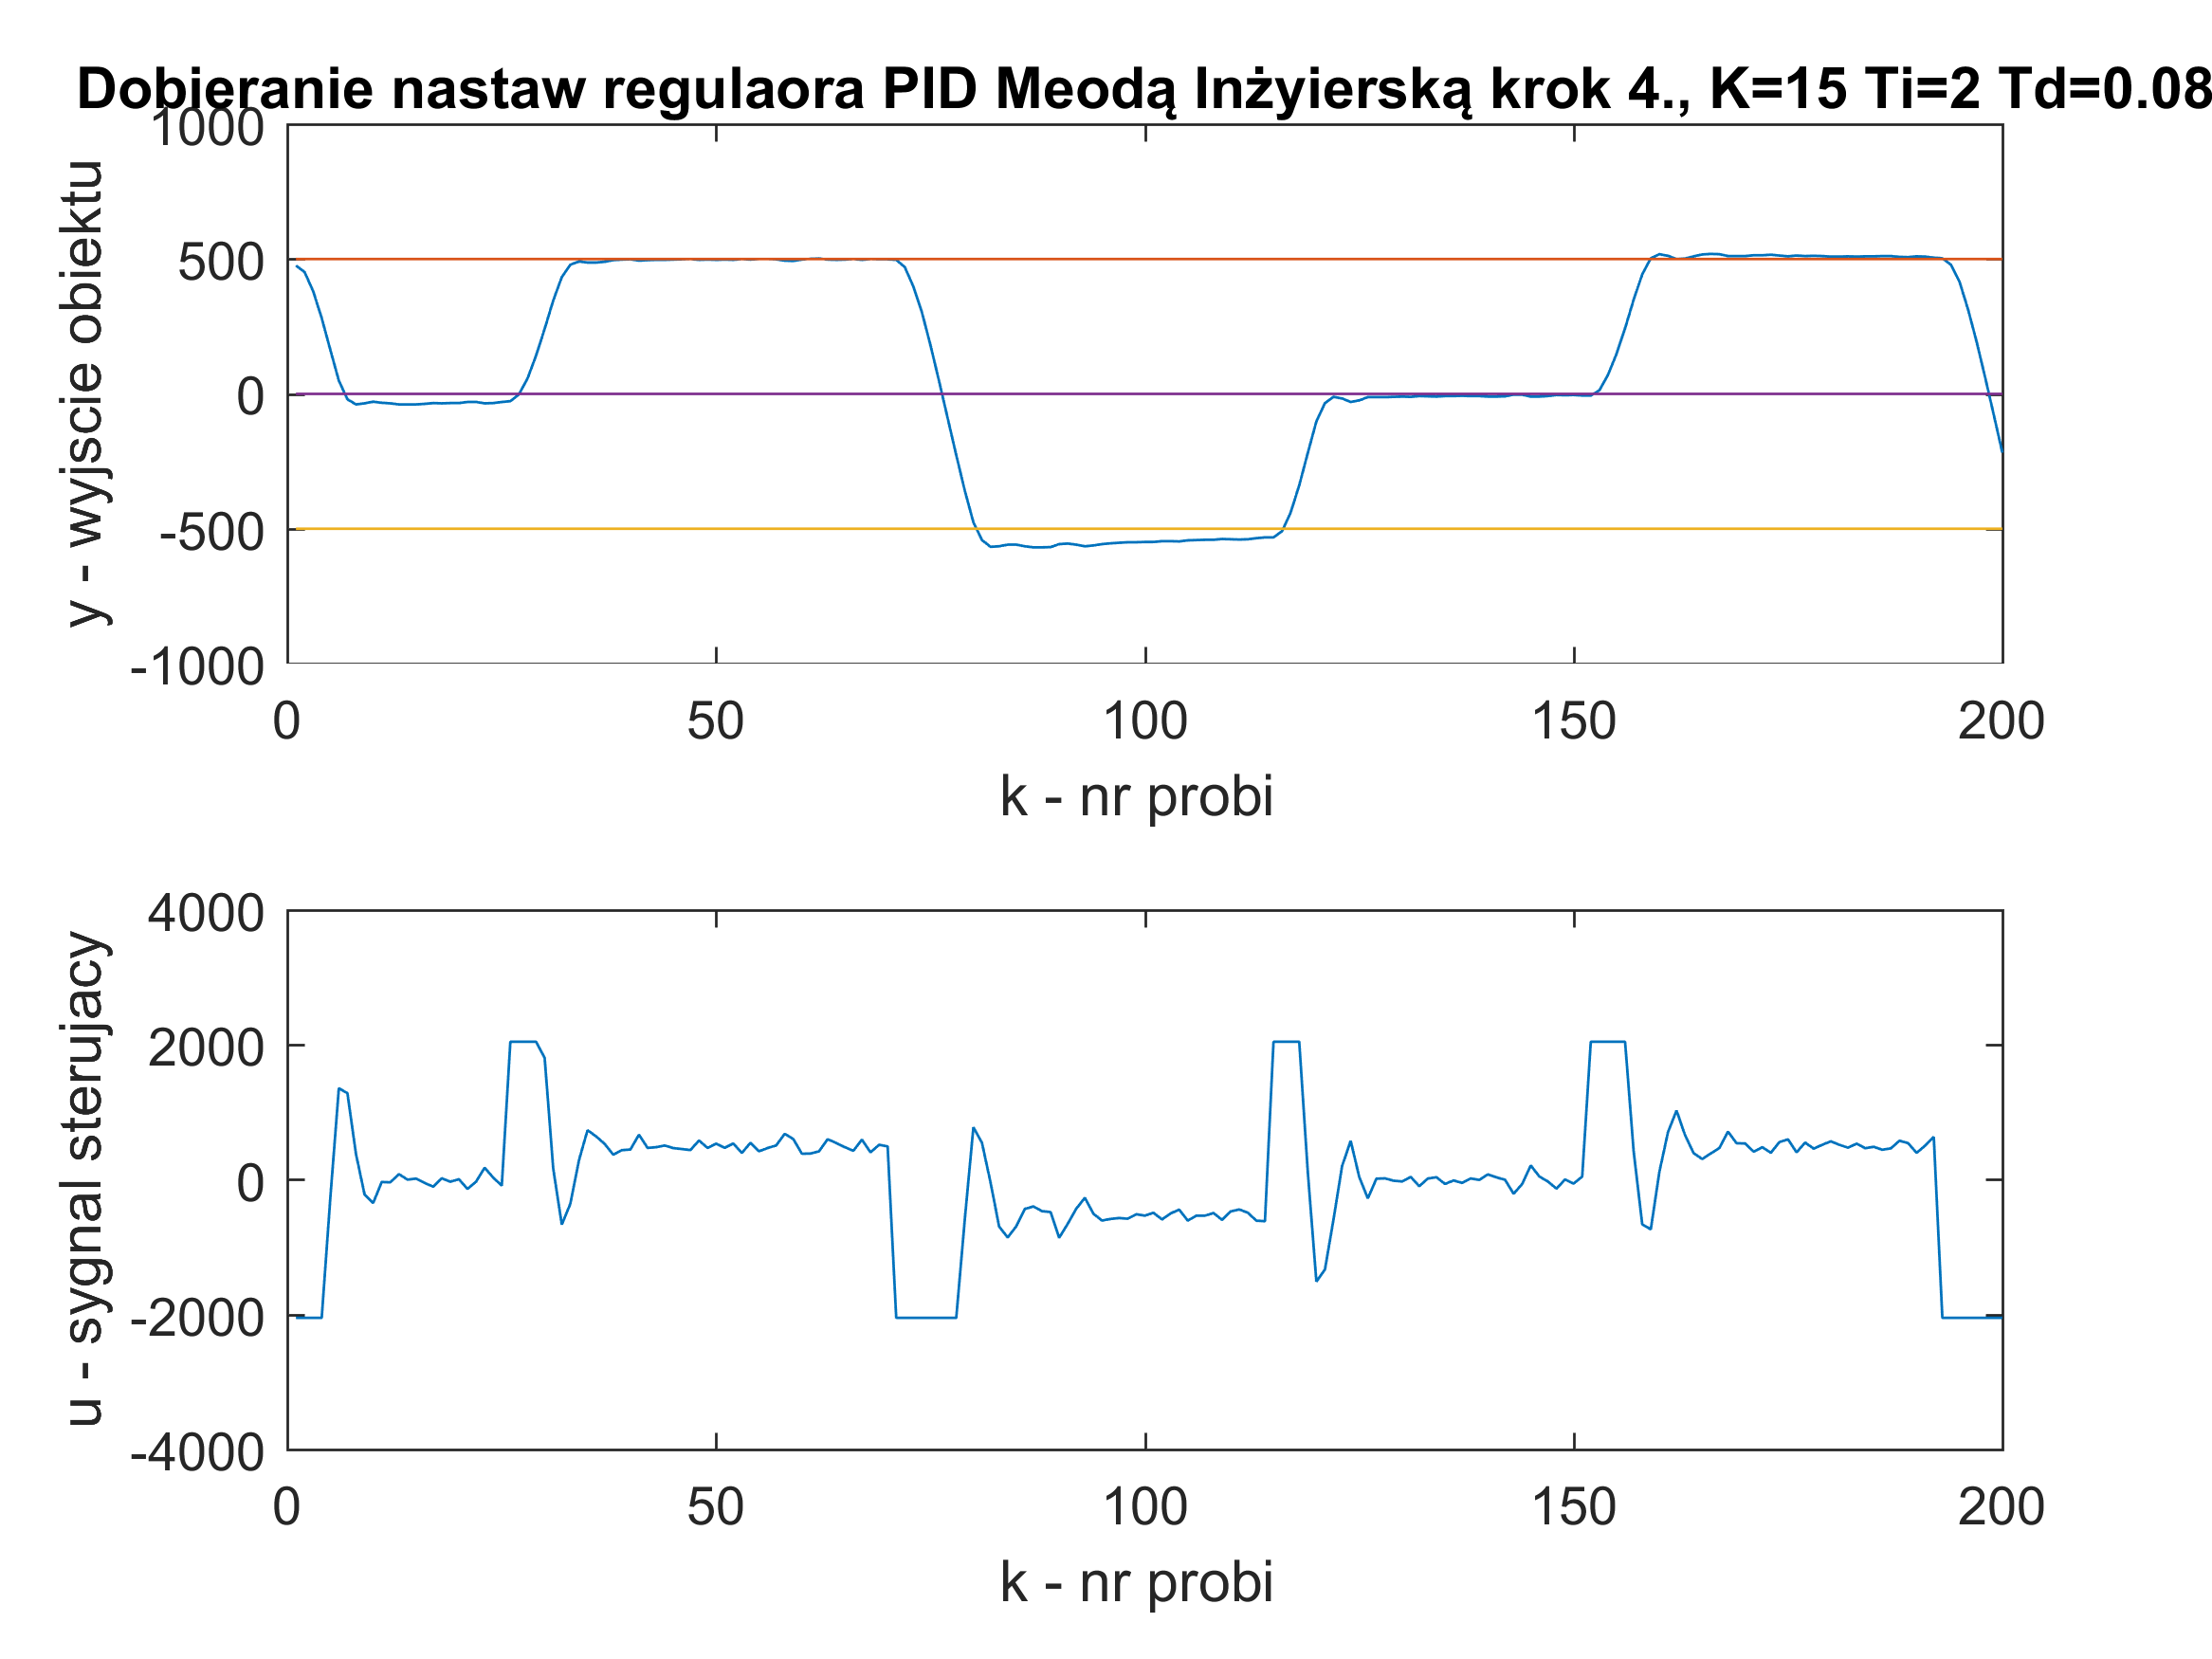
\includegraphics[width=0.9\linewidth]{MI_22}
	\caption{Wyjście obiektu przy $K=15, T_{I}=2, T_{D}=0,08 $  }
	\label{fig:MI_22}
\end{figure}
Z wykresu \ref{fig:MI_22} wynika, że zwiększenie stałej $K$ delikanie pogorszyło jakość regulaji, zwiększyły się oscylacje w okolicach wartości zadanej. Zmniejszenie stałej całkowania spowodowało wydłużenie czasu regulacji - przez dłuższy czas występuje zauważalny uchyb (wykres \ref{fig:MI_33}). Delikatny wzrost wpływu całki ( $T_{I}=1,8$) spowodował, że obiekt szybciej osiągnął zadane wartości. Z tego powodu wybrałyśmy następujące wartości parametrów regulatora PID metodą inżynierską:
\[K = 14\]
\[T_{i} = 1,8\]
\[T_{d} = 0,08\]
Sprawiają one, że występuje niewielkie przeregulowanie, a czas regulacji jest zadawalający. 
\begin{figure}[H]
	\centering
	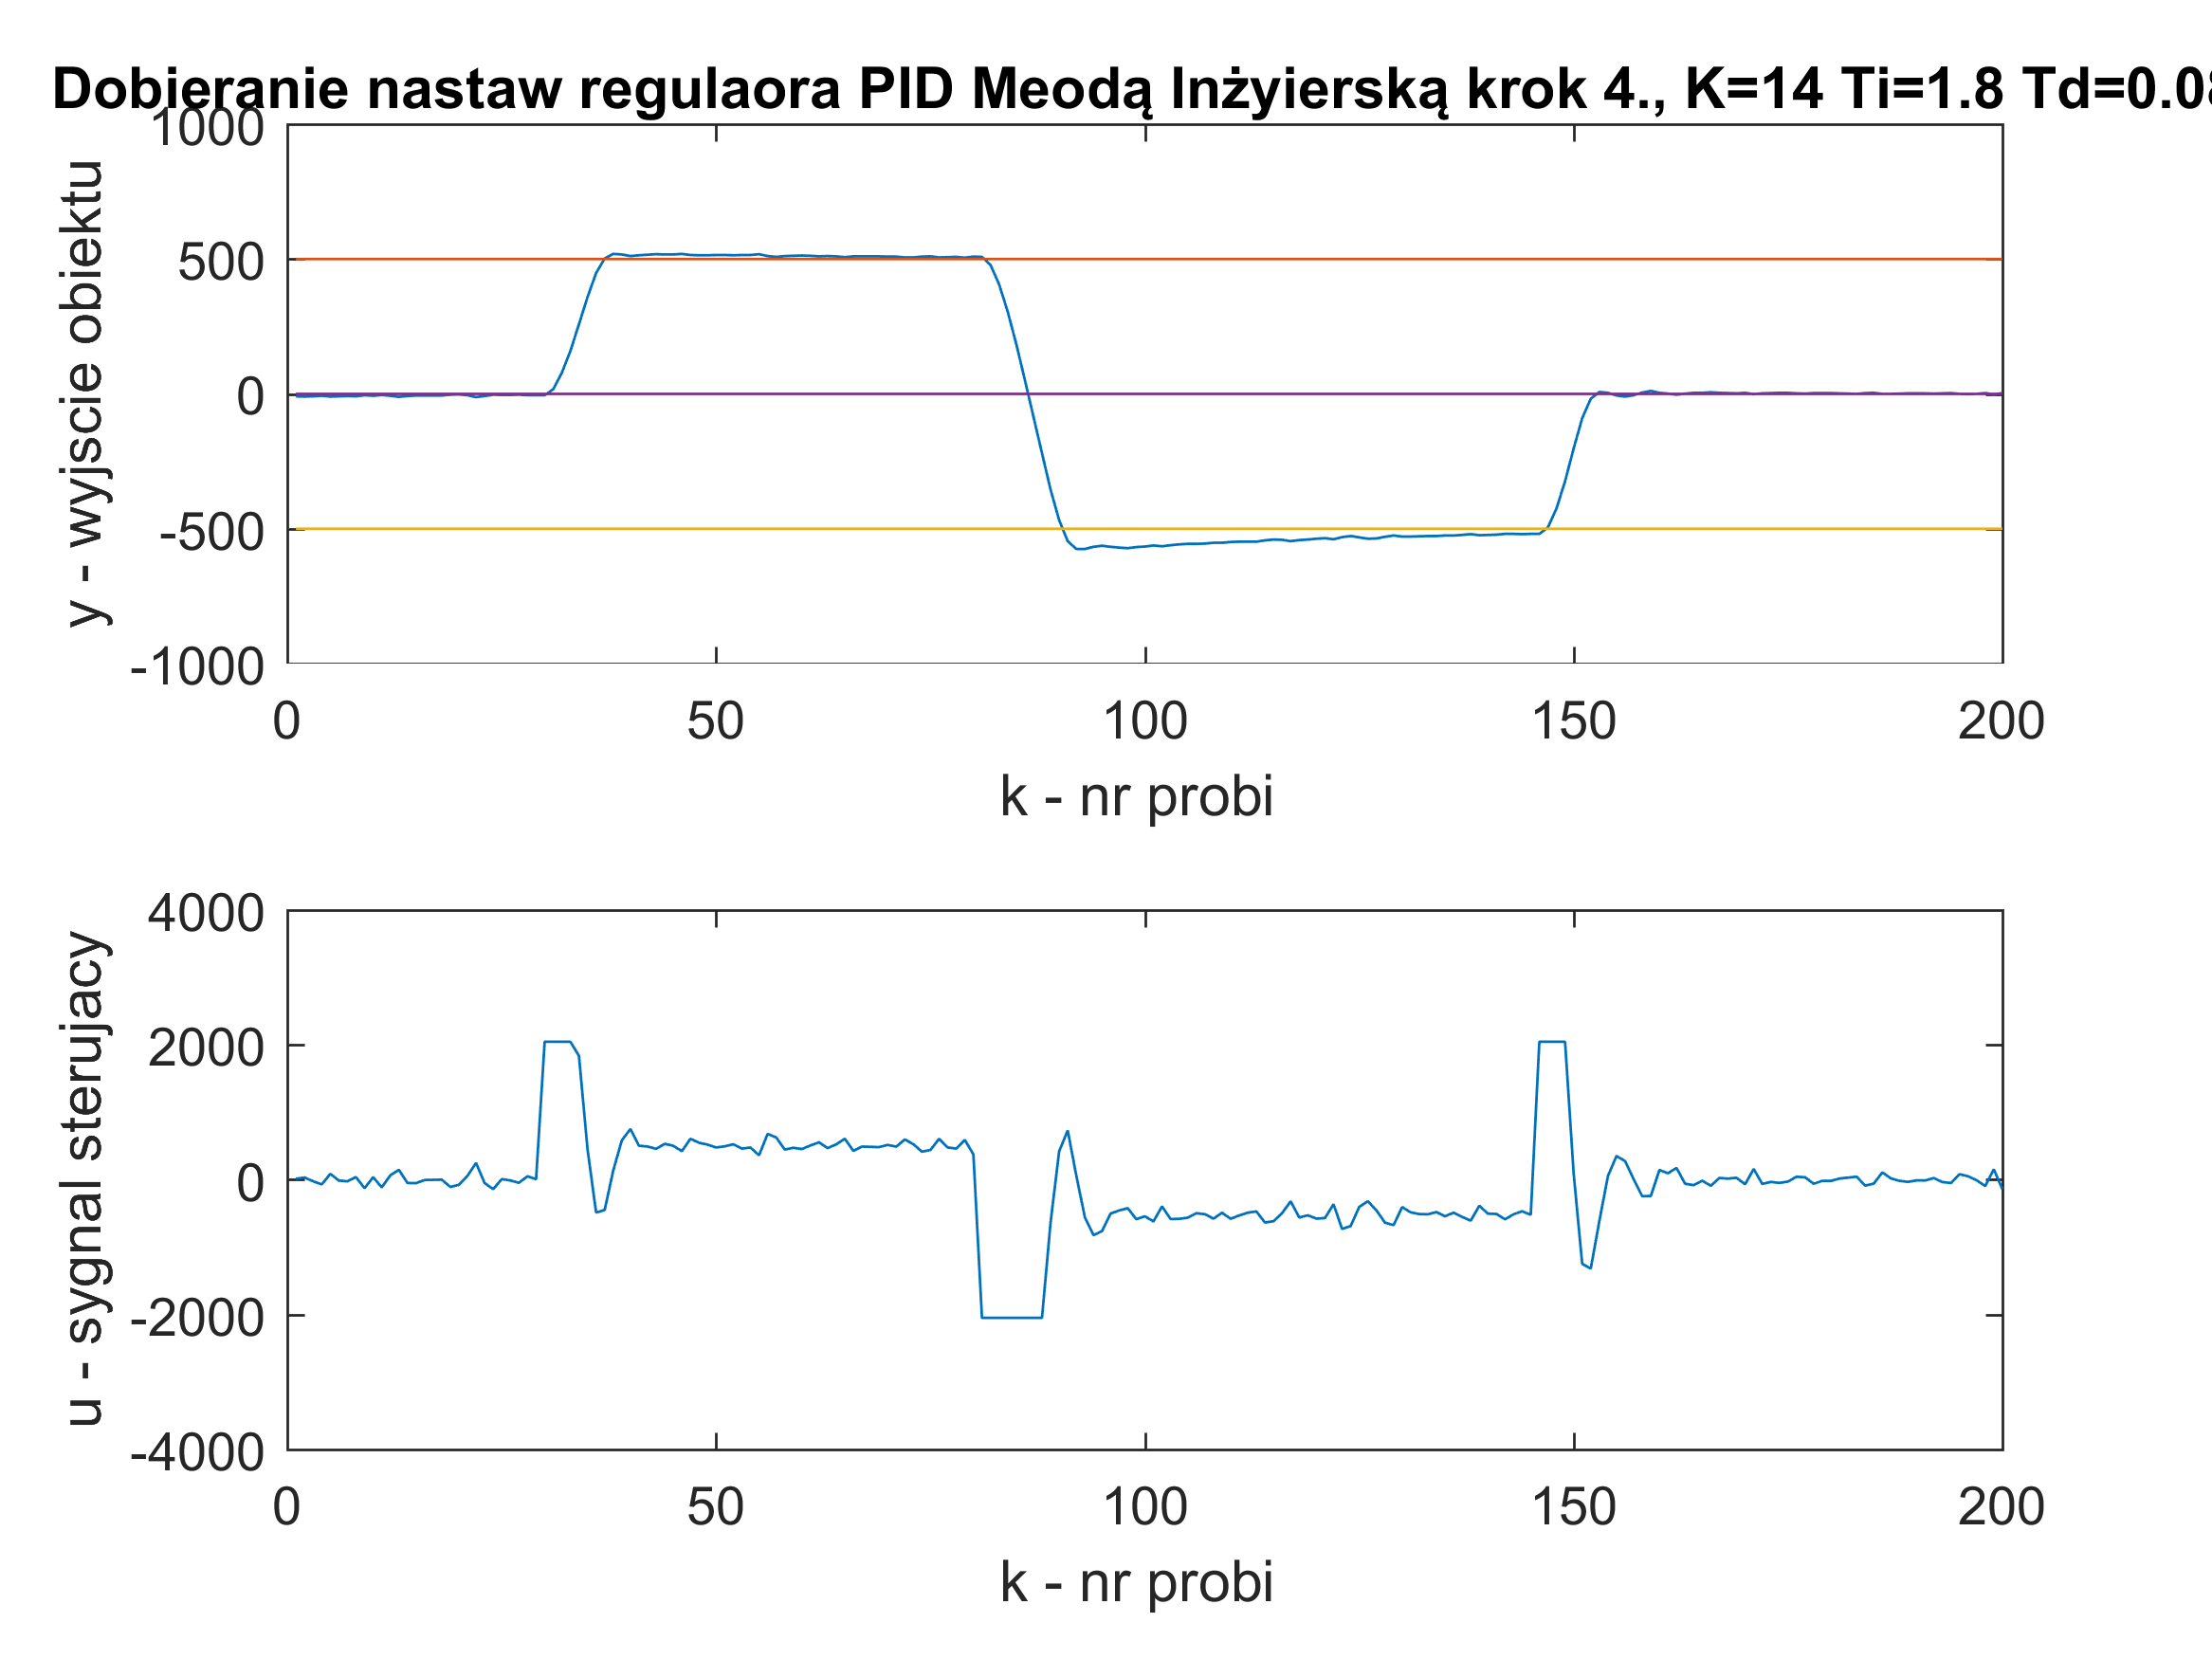
\includegraphics[width=0.9\linewidth]{MI_11}
	\caption{Przebieg sygnałów ostatecznie wybranego regulatora PID metodą inżynierską}
	\label{fig:MI_ost}
\end{figure}


\subsection{Porównanie wyników} \label{porownaj}
Mając dwa regulatory do wyboru, należy porównać je pod względem założonych kryteriów.

Przesterowanie można obliczyć ze wzoru:
\[K_0=\frac{y_{m}-y^{zad}}{y_{m}}\cdot 100\%\]
gdzie: \\
$y_{m}$ - jest maksymalną osiągniętą w trakcie eksperymentu wartością sygnału wyjściowego\\
$y^{zad}$ - jest zadaną wartością sygnału wyjściowego\\

Czas ustalenia $T_{ust}$ to czas od zmiany wartości sygnału zadanego, do chwili, gdy wartość  bezwzględna  uchybu  przestaje  przekraczać  pewną  przyjętą  niewielką  wartość $\epsilon$. \\
\[T_{ust}=(T_1-T_0)\cdot T\]
gdzie: \\
$T_1$ - chwila, w której wartość wyjściowa wchodzi w zakres wartości $y^{zad}-\epsilon$ do $y^{zad}+\epsilon$ i go nie opuszcza
$T_0$ - chwila zmiany wartości zadanej\\
$T$ - czas próbkowania\\

Wartości do obliczenia przesterowania i czasu narastania zostały odczytane z wykresów (Rysunki \ref{fig:ocenaPIDMI}, \ref{fig:ocenaZN}, \ref{fig:ocenaPIDMI_przereg},  \ref{fig:ocenaZN_przebieg}). Przyjmujemy, że $\epsilon = 7\% \cdot y^{zad}$. Czas próbkowania $T = 0,05s$. Wartość zadana $y^{zad}$ jest równa 500. Z wykresów odczytujemy $y_{m} = 519$ dla metody inżynierskiej i  $y_{m} = 539$ dla metody Z-N. Dla metody inżynierskiej $T_0 = 29$, $T_1 = 37$, a dla metody Zieglera-Nicholsa $T_0 = 174$, $T_1 = 193$.



\begin{figure}[H]
	\centering
	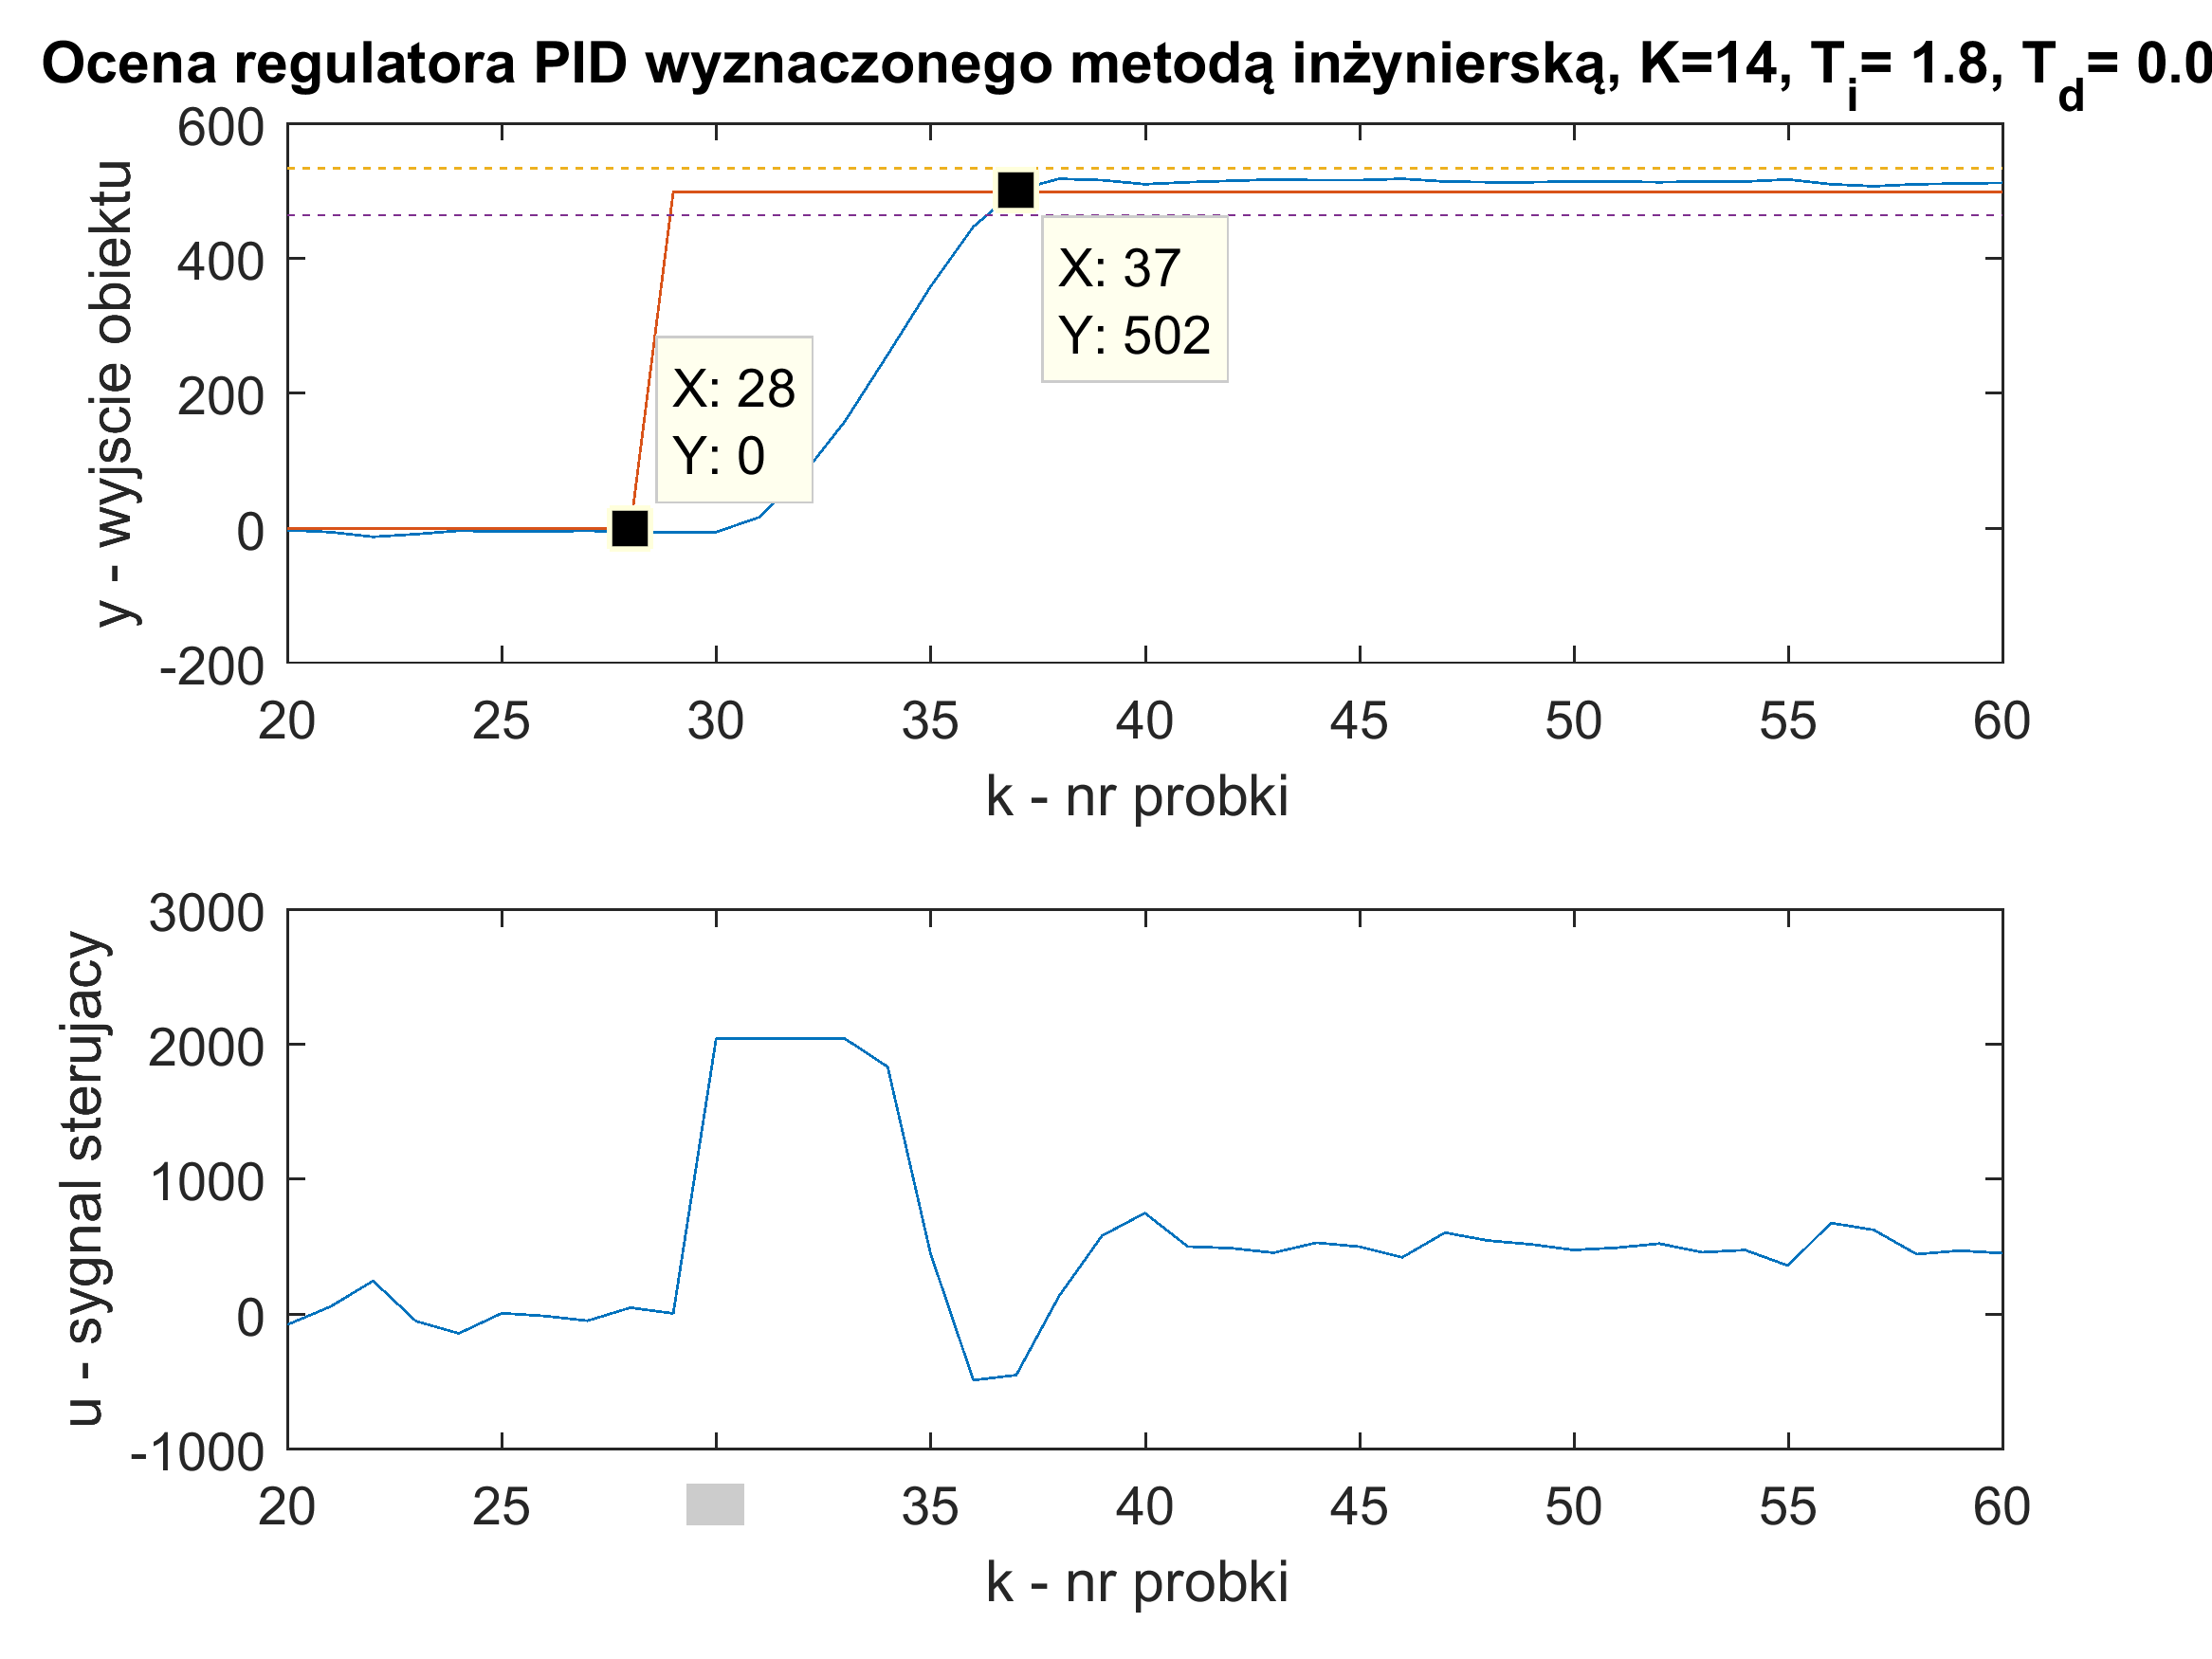
\includegraphics[width=0.9\linewidth]{ocenaPIDMI}
	\caption{Ocena regulatora wyznaczonego metodą inżynierską: $K=14, T_{i}=1,8, T_{d}=0,08$}
	\label{fig:ocenaPIDMI}
\end{figure}
\begin{figure}[H]
	\centering
	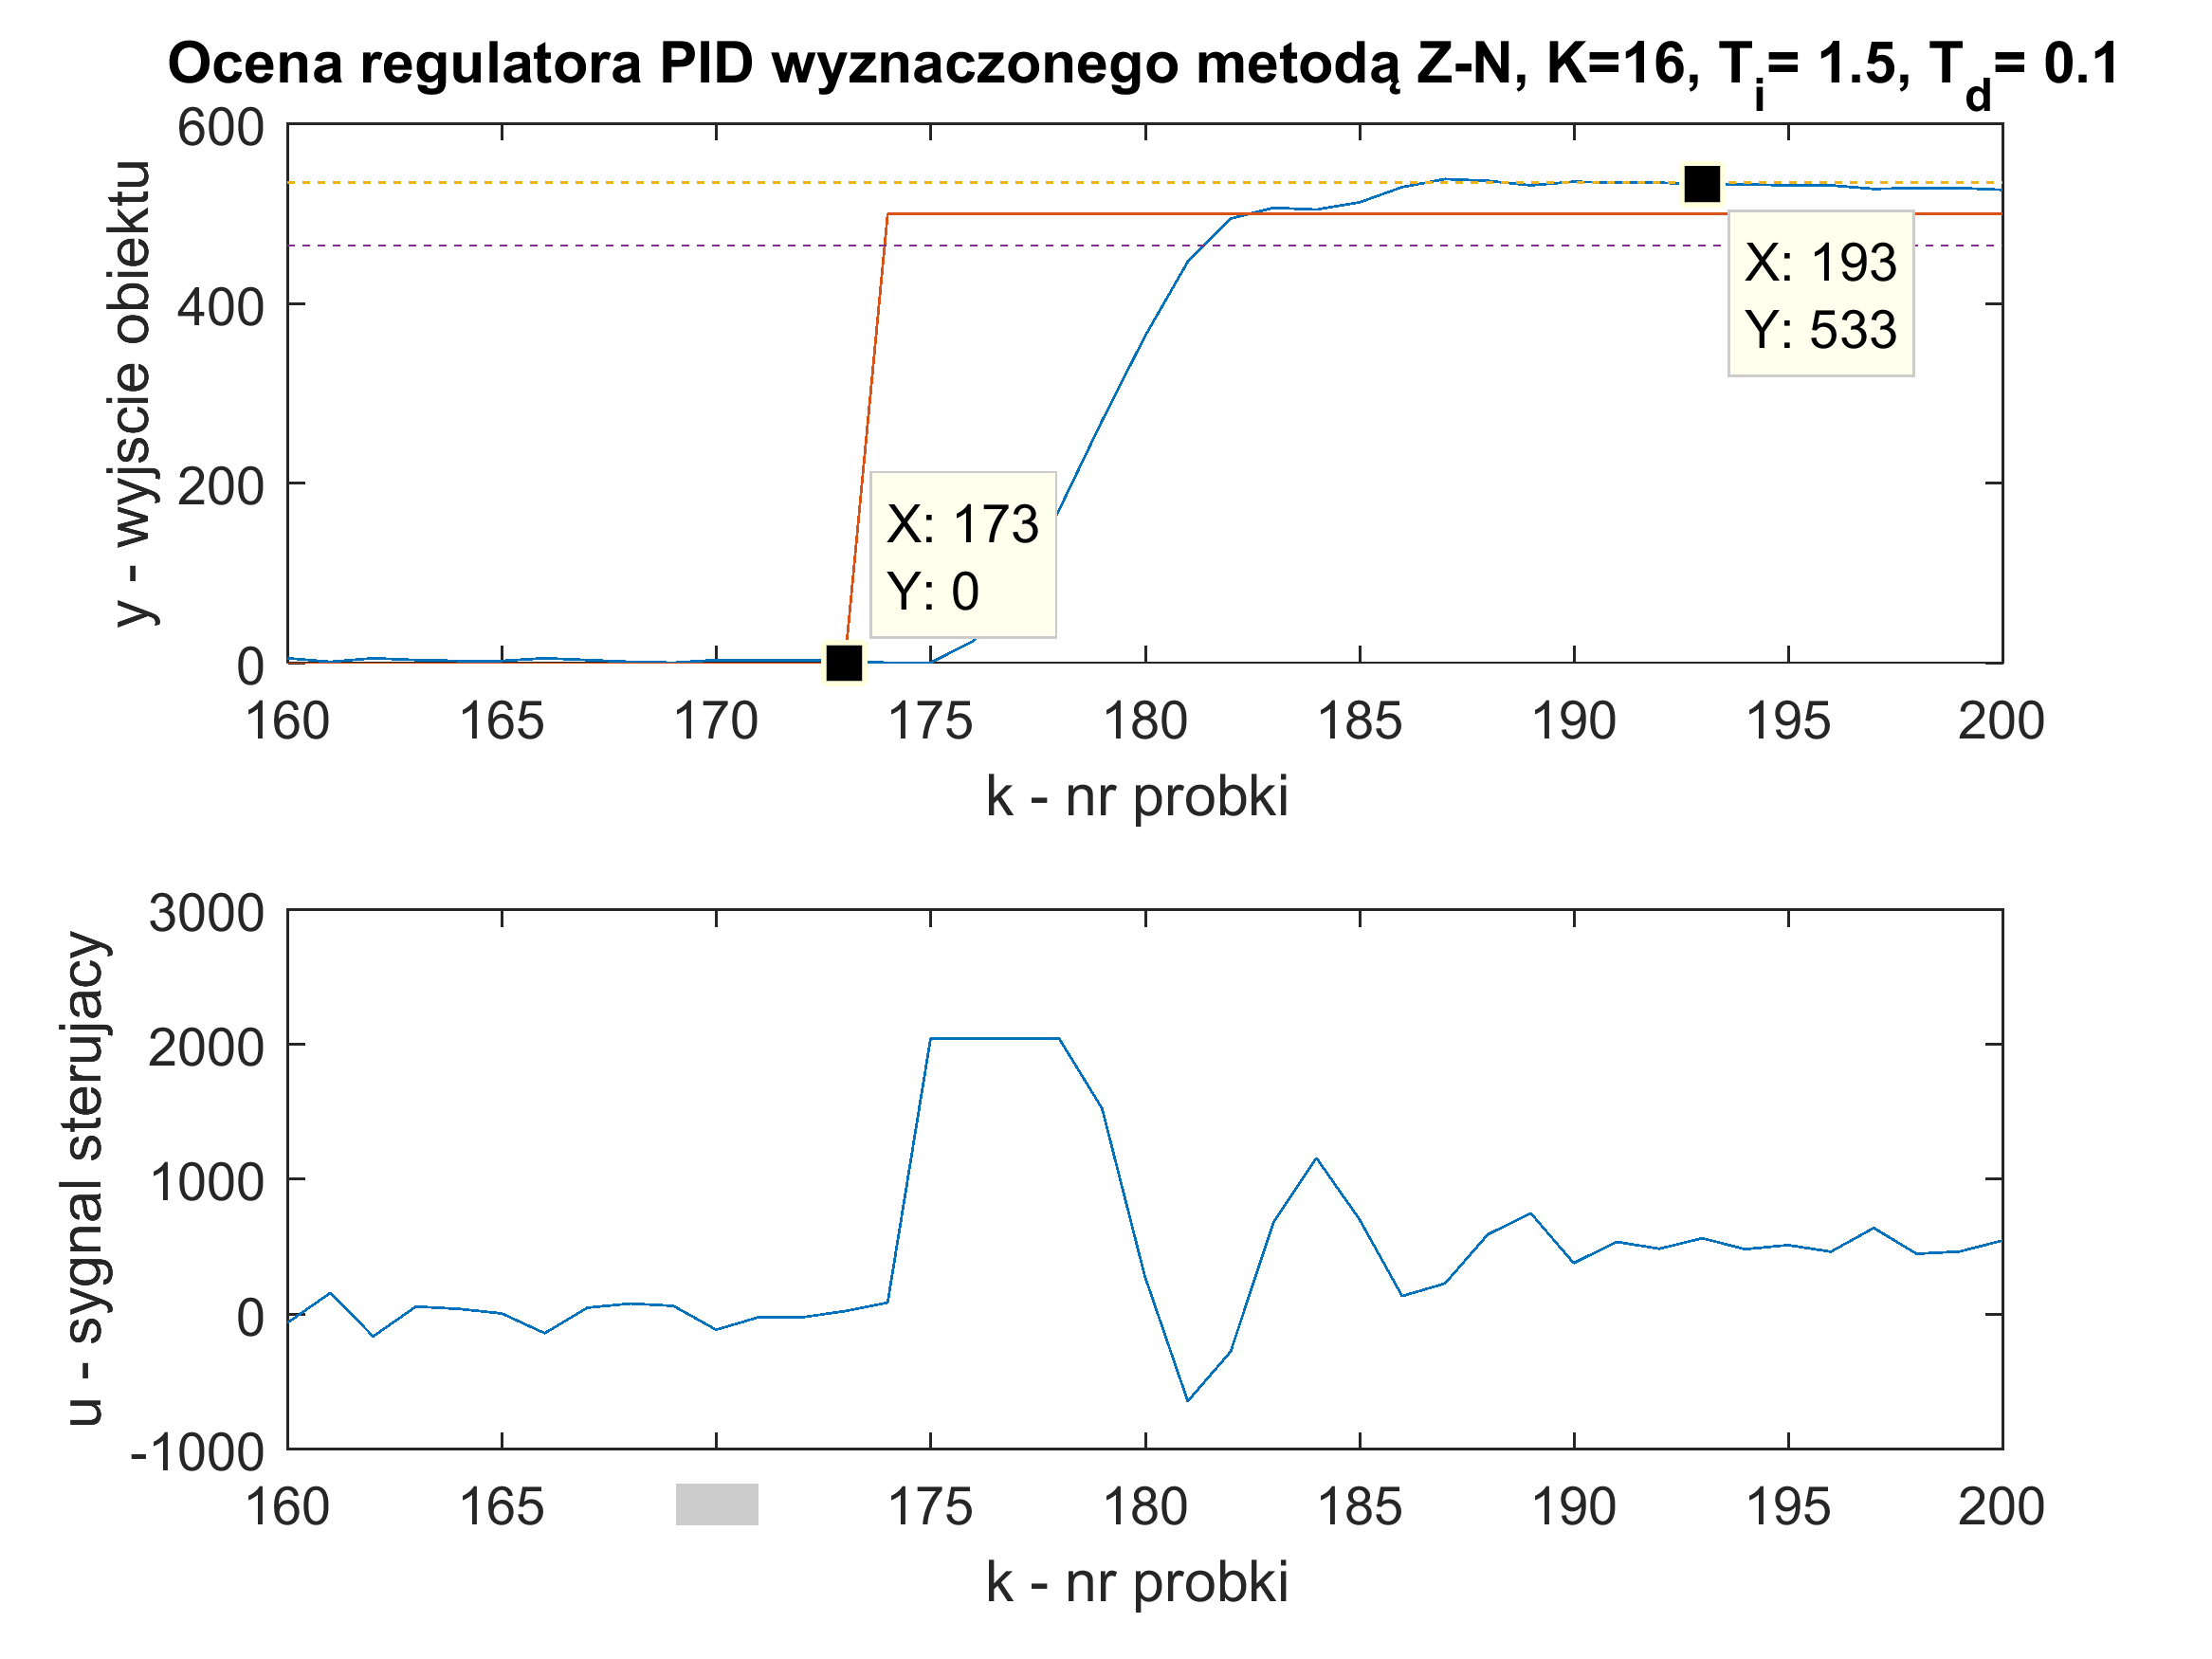
\includegraphics[width=0.9\linewidth]{ocenaPIDZN}
	\caption{Ocena regulatora wyznaczonego metodą Z-N: $K=16, T_{i}=1,5, T_{d}=0,1$}
	\label{fig:ocenaZN}
\end{figure}

\begin{figure}[H]
	\centering
	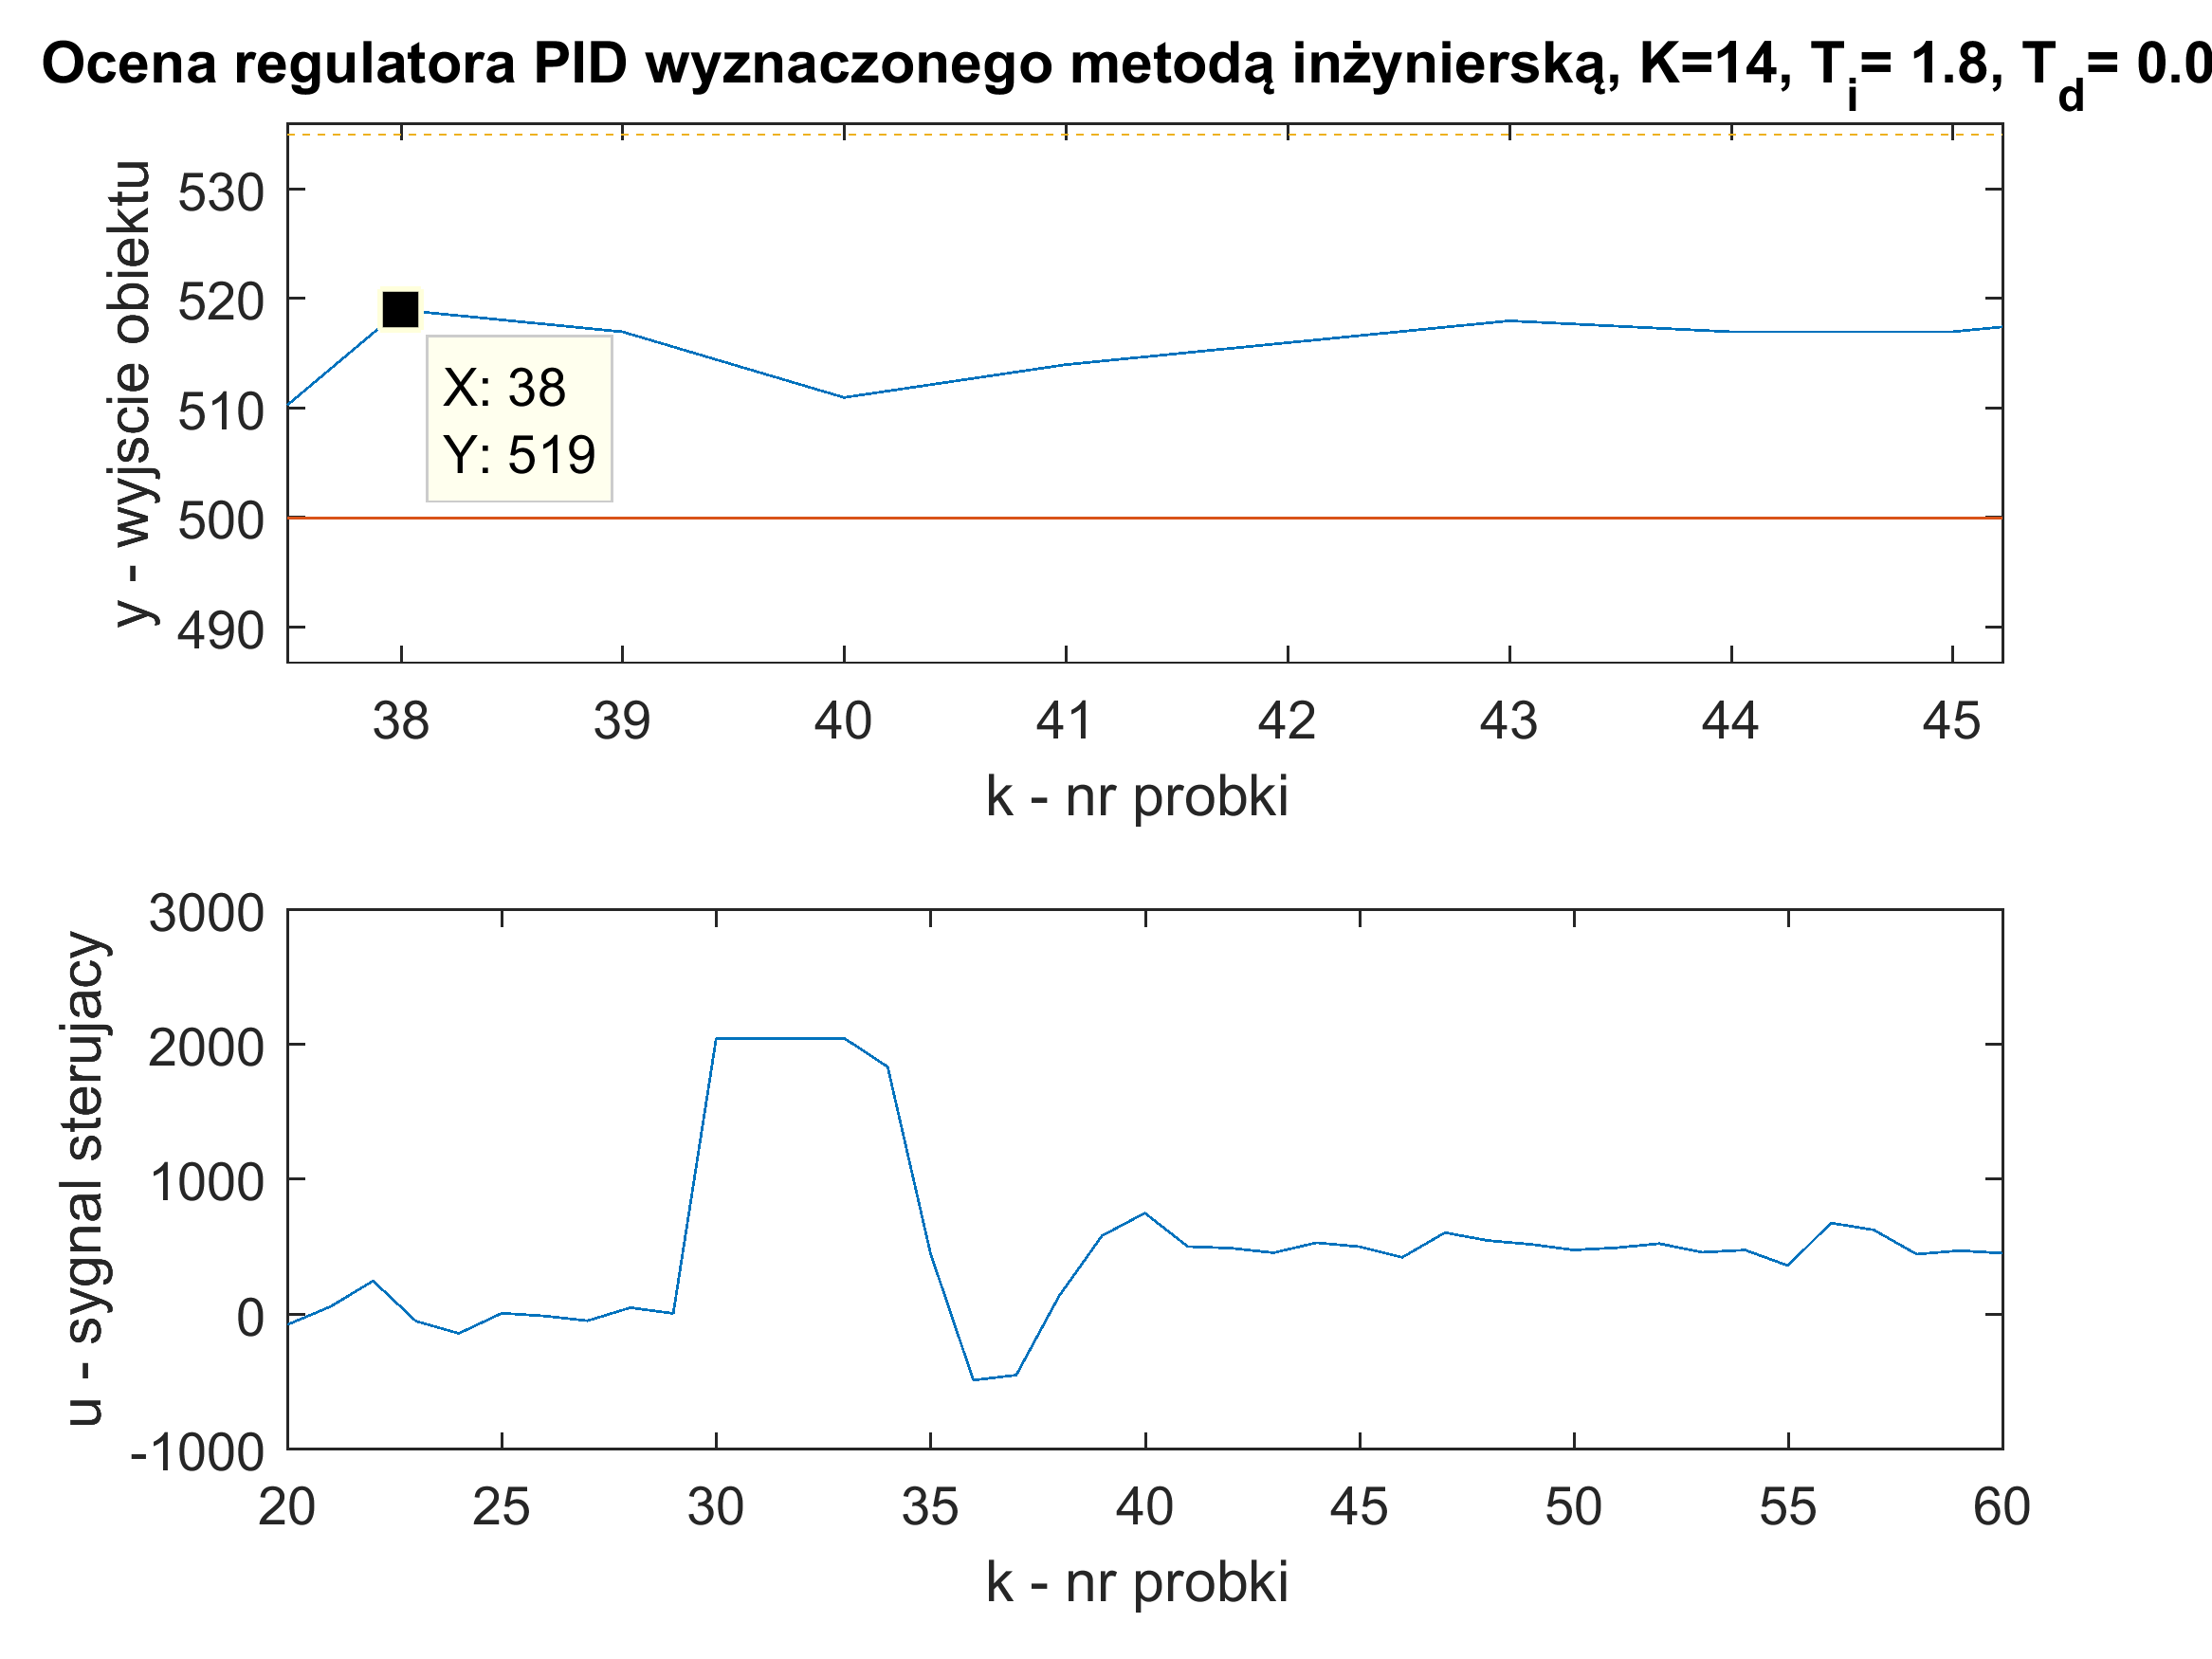
\includegraphics[width=0.9\linewidth]{ocenaPIDMI_przereg}
	\caption{Ocena regulatora wyznaczonego metodą inżynierską: $K=14, T_{i}=1,8, T_{d}=0,08$}
	\label{fig:ocenaPIDMI_przereg}
\end{figure}
\begin{figure}[H]
	\centering
	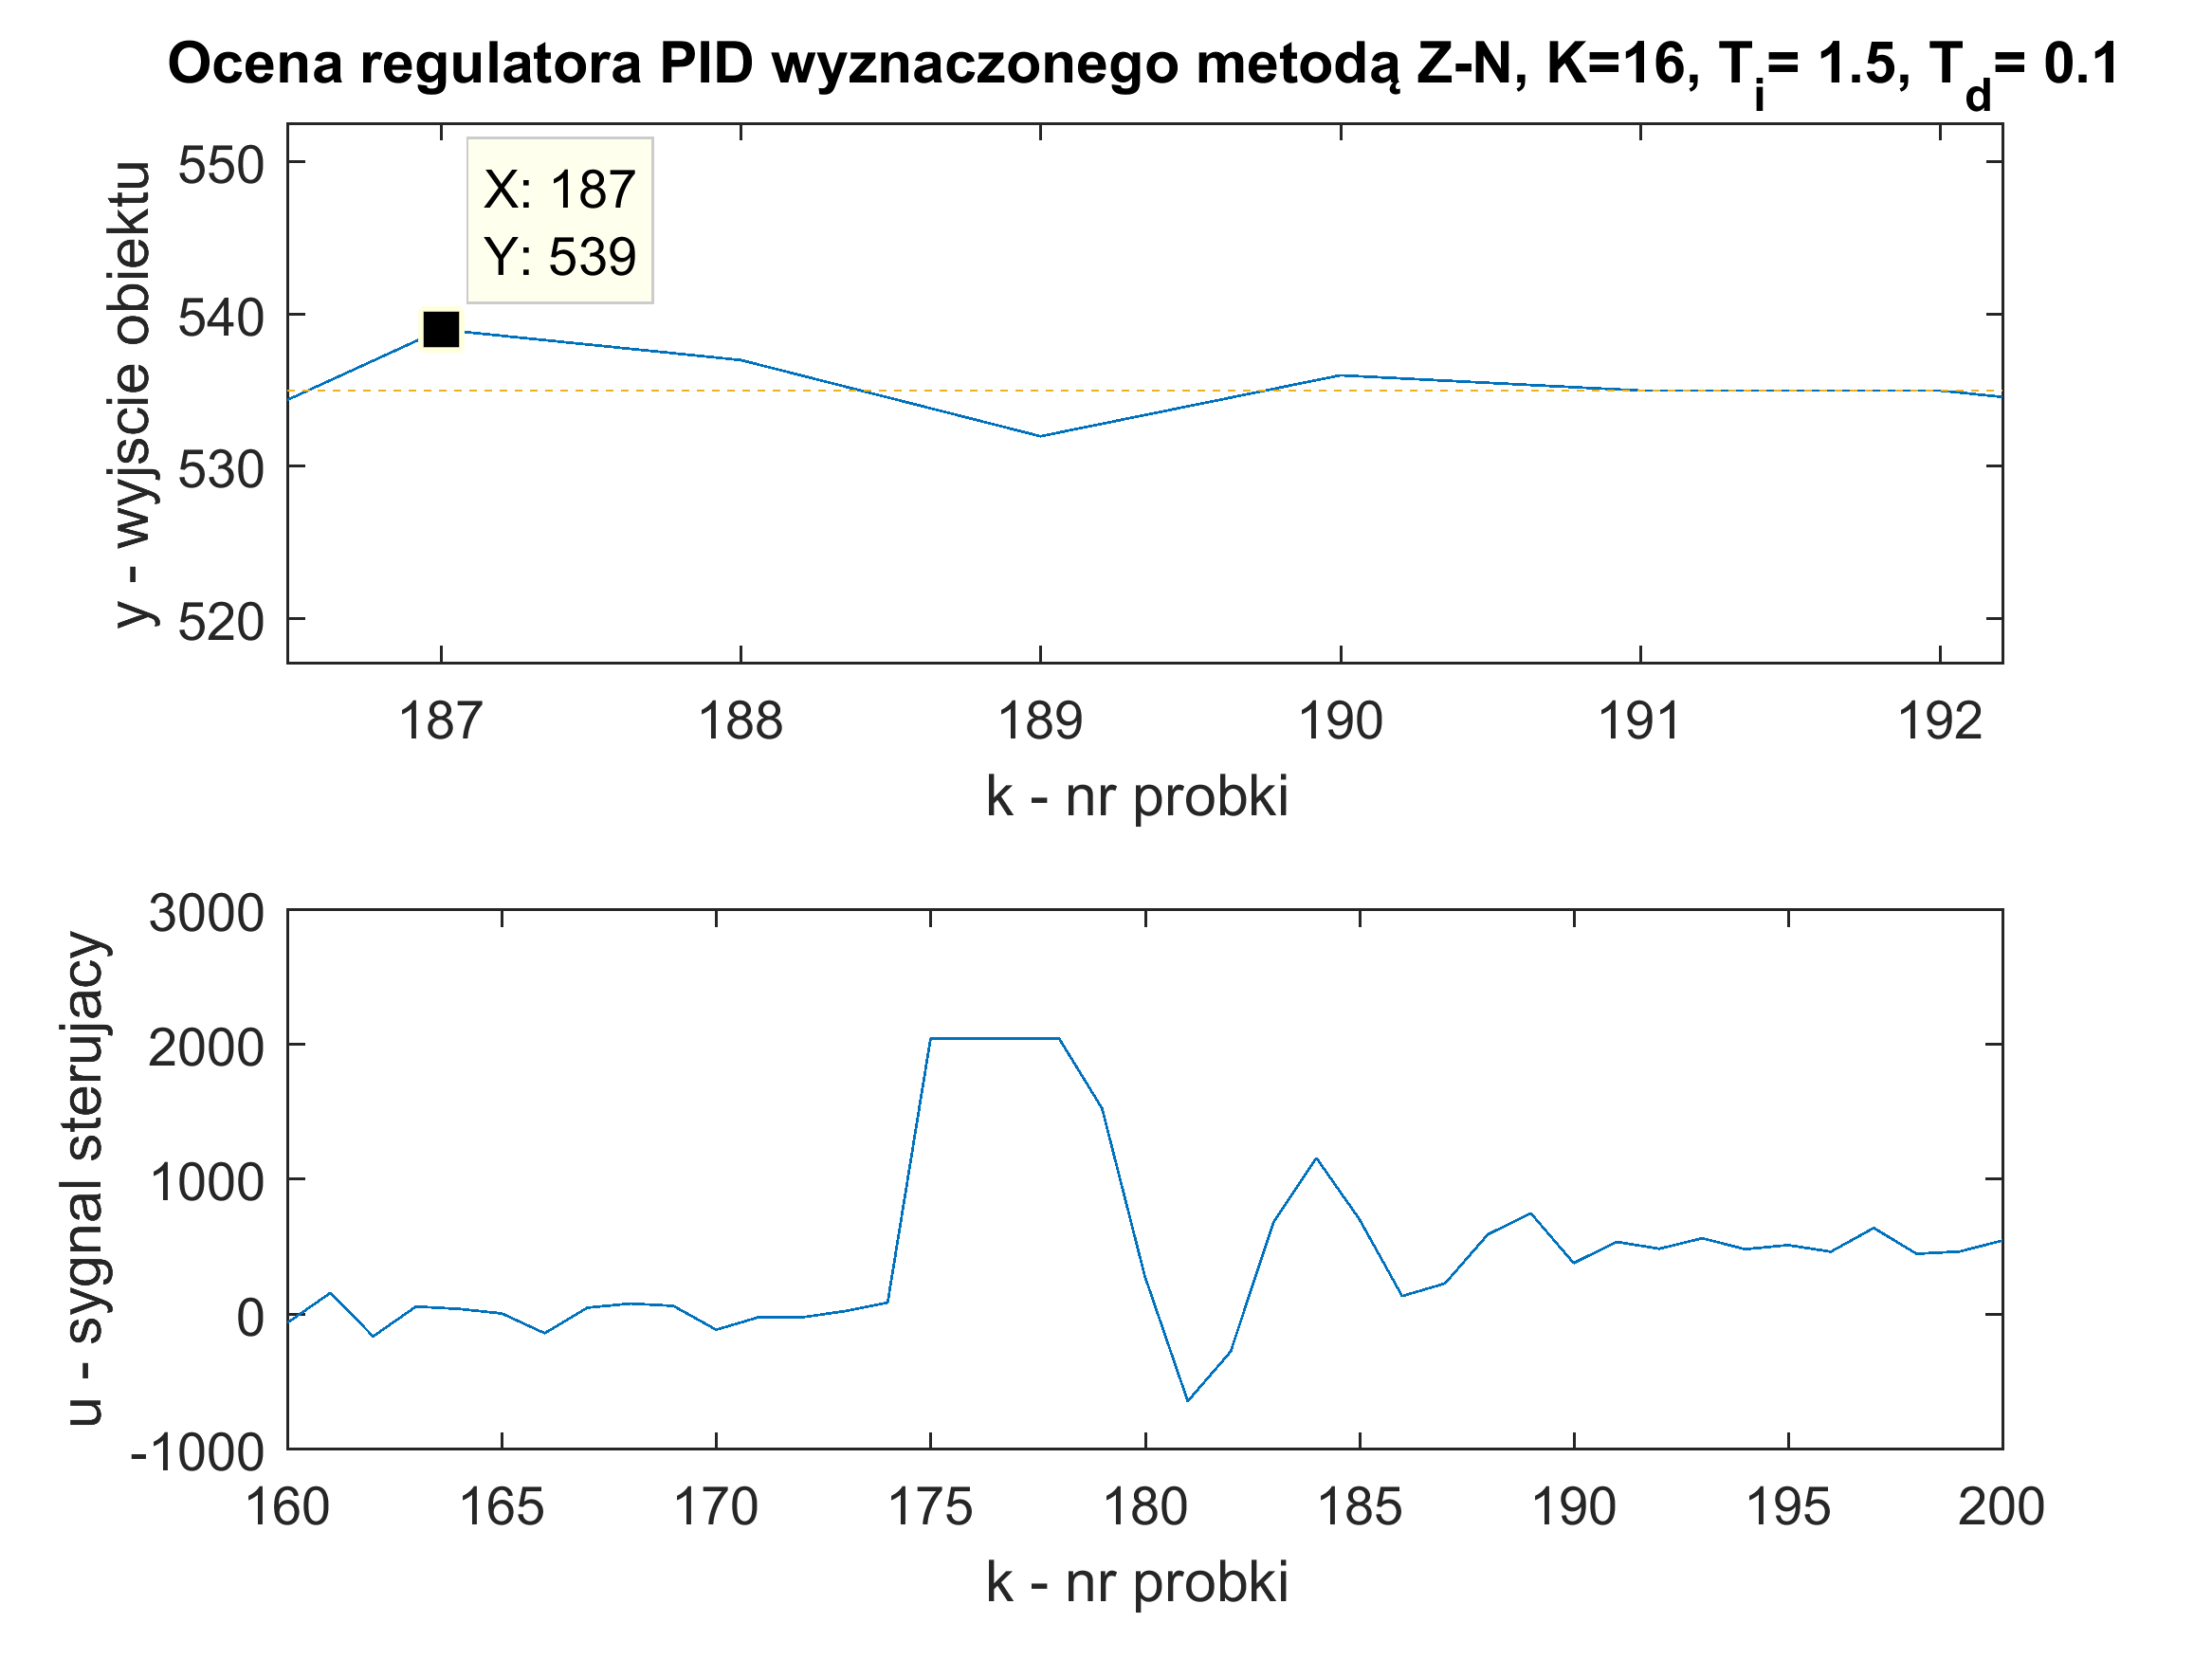
\includegraphics[width=0.9\linewidth]{ocenaPIDZN_przebieg}
	\caption{Ocena regulatora wyznaczonego metodą Z-N: $K=16, T_{i}=1,5, T_{d}=0,1$}
	\label{fig:ocenaZN_przebieg}
\end{figure}


\begin{table}[h]
		\caption{Porównanie metod: inżynierskiej i Zieglera-Nicholsa} 
\begin{center}
	\begin{tabular}{|c|c|c|c|}  \hline
		Metoda & przesterowanie  & czas ustalenia & oscylacje \\ \hline
		inżynierska & $3,8\%$  & $0,4s$ & $-$ \\ \hline      
		Z-N & $7,8\%$  & $0,95s$ & $-$ \\ \hline 	
	\end{tabular}
\end{center} 
\end{table}

Regulatory wyznaczone różnymi metodami maja różne nastawy i co za tym idzie inne trajektorie sygnału wyjściowego. Dla obu nie występują oscylacje przy dążeniu do wartości zadanej ani uchyb ustalony, co było podstawowym przyjętym przez nas kryterium. Różnice występują za to przy przesterowaniu i szybkości dążenia do wartości zadanej. Przesterowanie dla regulatora z metody inżynierskiej ($3,8\%$) jest około 2 razy mniejsze niż dla regulatora z metody Zieglera-Nicholsa ($7,8\%$). Podobna różnica jest przy czasie ustalenia. Regulator z metody inżynierskiej dwa razy szybciej ($0,4s$) niż regulator z metody Z-N ($0,95s$) dociera wartością sygnału wyjściowego do ustalonego zakresu. Metoda Z-N dałaby krótszy czas ustalenia gdyby regulator szybciej odcałkowywał wartość sygnału wyjściowego po osiągnięciu maksymalnej wartości sygnału sterującego, należałoby zaimplementować algorytm anty-windup. Regulator z metody inżynierskiej dłuzej osiąga najwyższą wartość sygnału wyjściowego, ale potem bardzo szybko wpada w ustalony zakres $y^{zad}-\epsilon$ do $y^{zad}+\epsilon$. Poza tym oba wykresy sygnału wyjściowego mają gładki przebieg bez znaczących oscylacji oraz podobny sygnał sterujący.

Lepszym regulatorem wedle przyjętych kryteriów okazał się regulator wyznaczony metodą inżynierską. Regulator wyznaczony z metody Z-N ma za duże przesterowanie w stosunku do przyjętych przez nas kryteriów i ma dłuższy czas ustalenia.

\subsection{Anty-windup}
Brak uwzględnienia ograniczeń sygnału sterującego wpływa na powstanie przeregulowań. Można to zauważyć szczególnie na wykresie \ref{fig:MI_ost}, gdzie przy zmianie wartości zadanej z 500 na -500 układ przez jakiś czas wysyłał graniczną wartość sterowania. Z  powodu "odcałkowywania" sygnału sterującego (po osiągnięciu wartości granicznej) wartość wyjścia stabilizowała się przez dłuższy czas. Aby zapobiec temu zjawisku do składowej całkującej należy w jakiś sposób przekazać informację o wartości sterowania rzeczywiście wysłanej na obiekt. Realizowane jest to poprzez dodanie do składowej całkującej pewnej stałej przemnożonej przez różnicę wysłanego sterowania z sterowaniem obliczonym z prawa regulacji:
\[u_{I}(k)=u_{I}(k-1)+\frac{K}{T_{I}} \cdot T\cdot\frac{e(k-1)+e(k)}{2}+\frac{T}{T_{v}}\cdot(u_{w}(k-1)-u(k-1))\]

$T_{v}$  jest parametrem algorytmu anti-windup, $u_{w}(k-1)$ jest watością sterowania wysłaną na obiekt po uwzględnieniu ograniczeń w poprzedniej próbce, a $u(k-1)$ wartością sterowania wyznaczoną przez prawo regulacji w poprzedniej chwili czasu. Można zauważyć, że algorytm ten ma wpływ na sterowanie tylko, jeśli wartości sterowania natkną się na ograniczenia.\\
Z uwagi na  wybranie przez nas regulatora PID z niewielkim czasem zdwojenia eksperymenty przeprowadzane były dla zmian wartości zadanej ze zbioru $\{-1900, 0, 1900\}$. Dla zmian wartości zadanej ze zbioru $\{-500, 0, 500\}$, prawo regulacji za krótko wyznaczało sygnał sterujący większy od ograniczeń, aby zauważyć widoczne różnice przy wprowadzeniu anty-winupu. 

\begin{figure}[H]
	\centering
	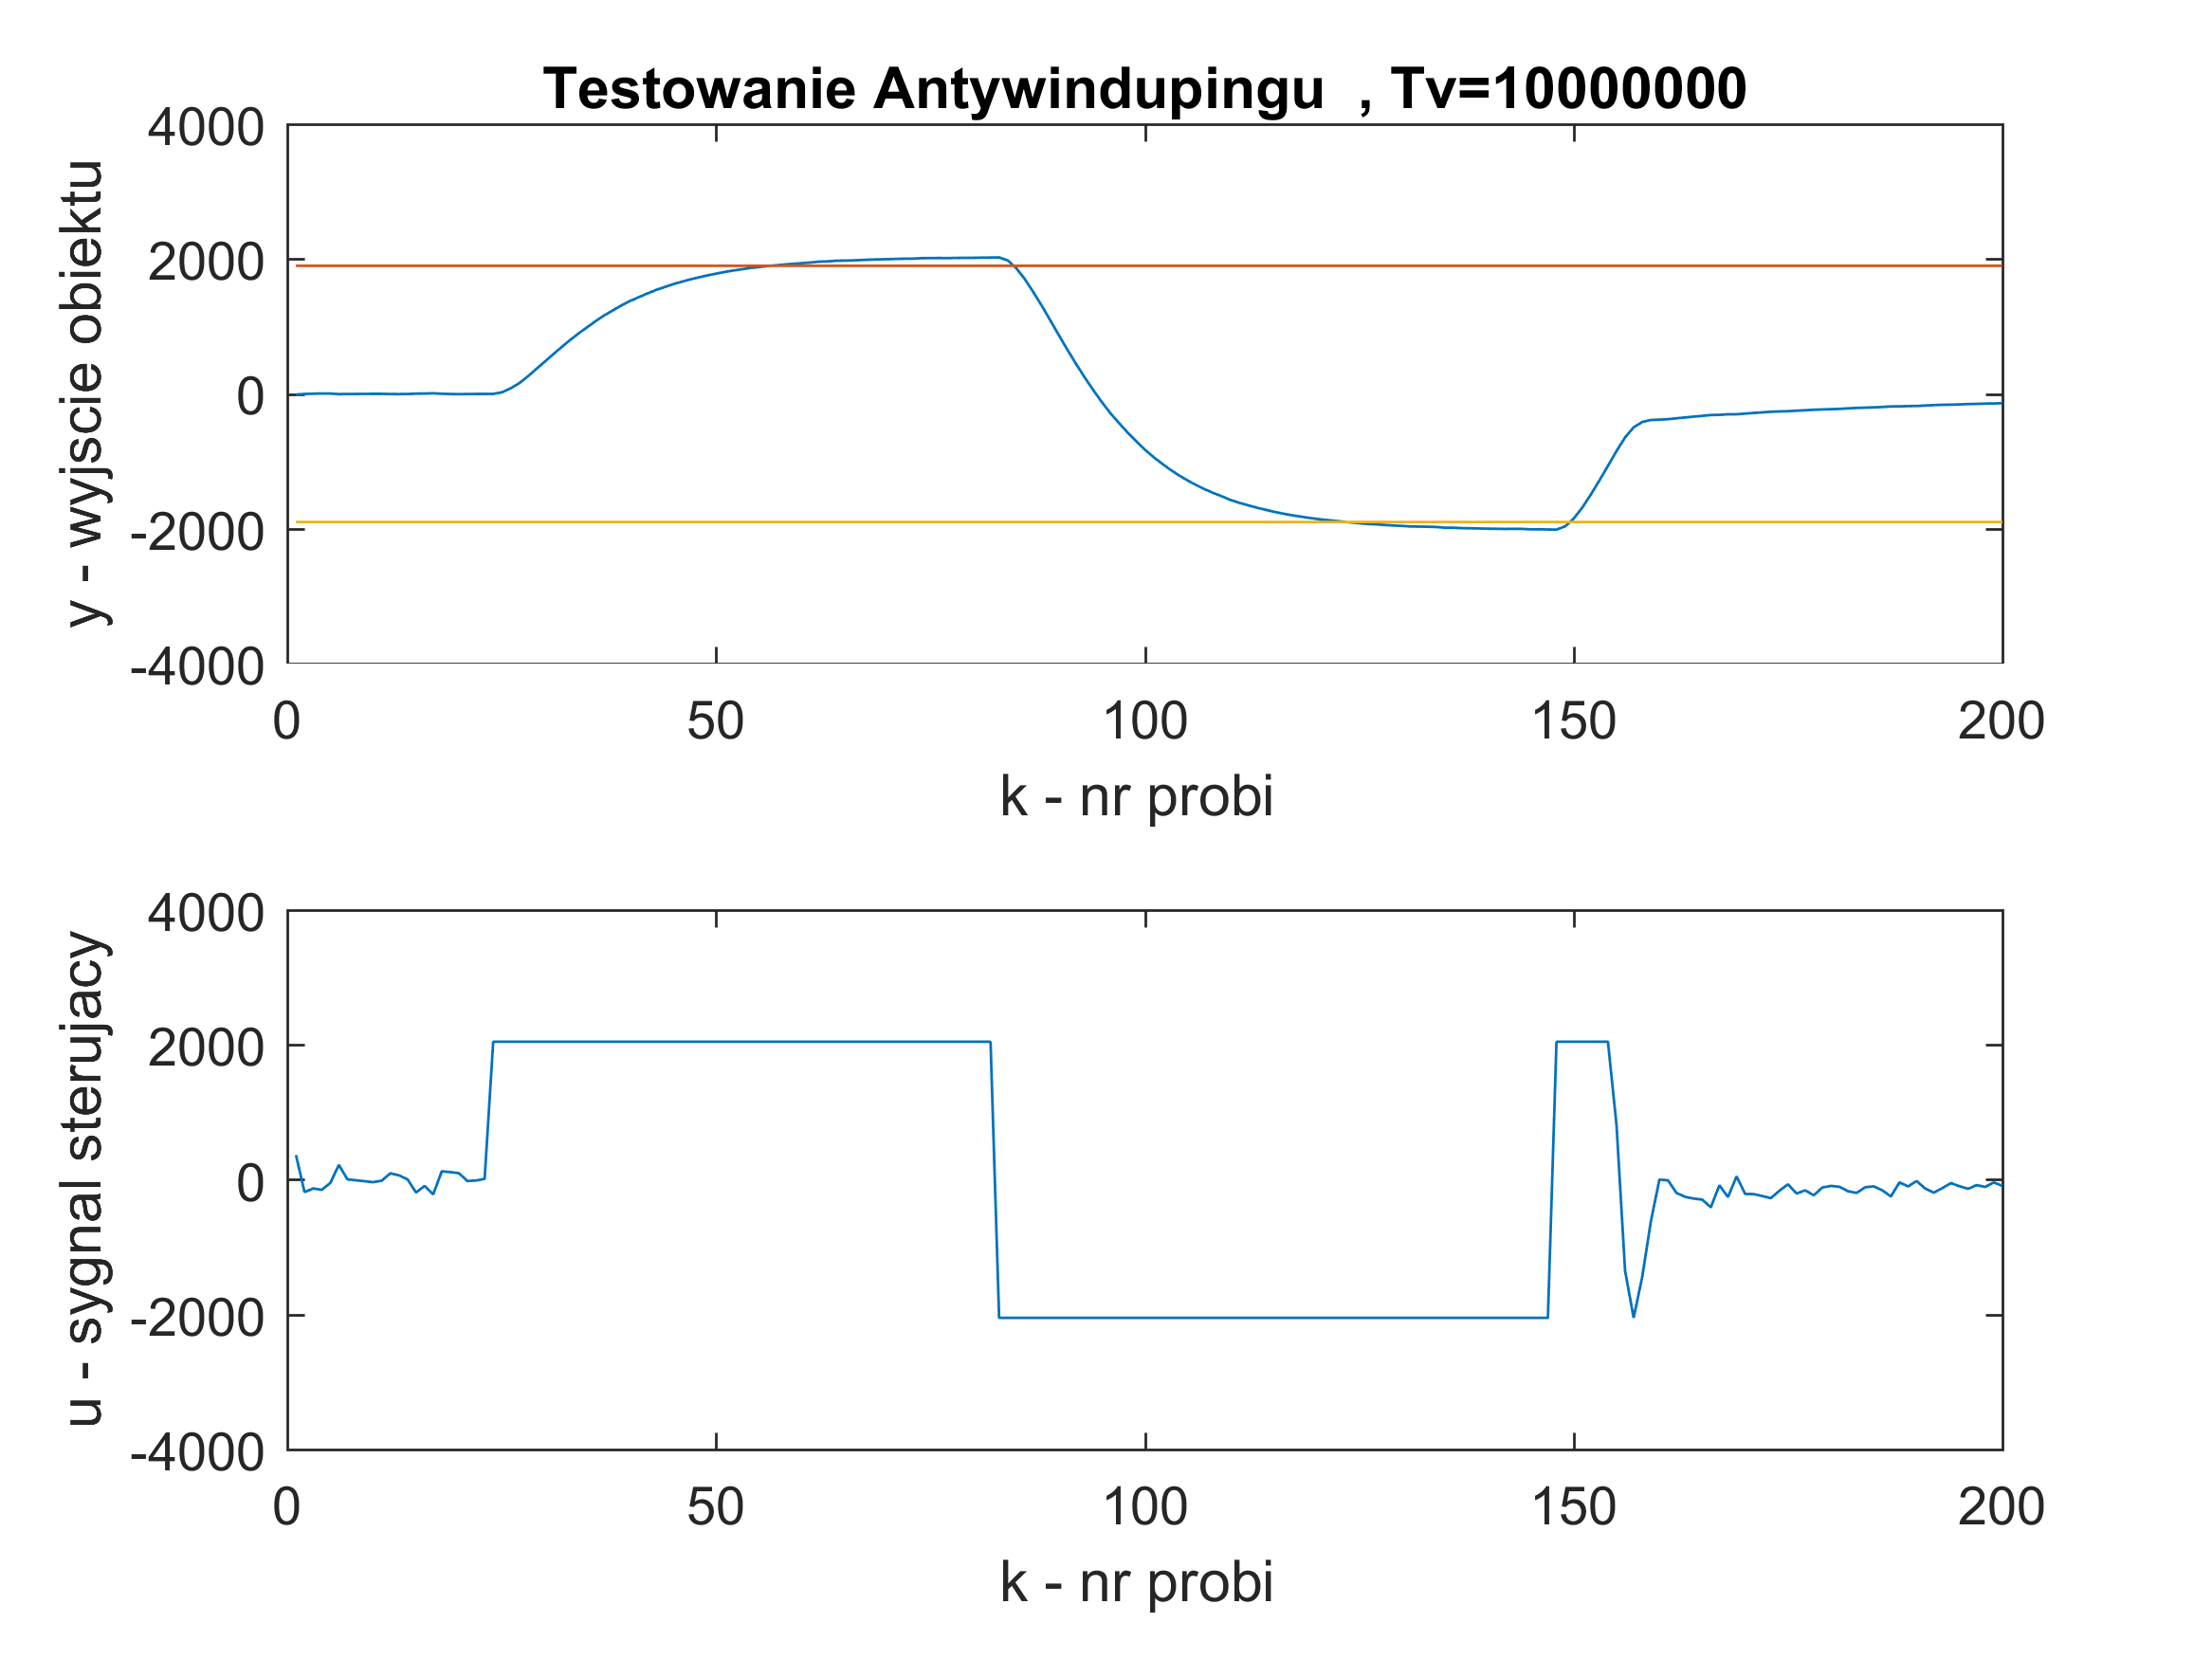
\includegraphics[width=0.9\linewidth]{awbez}
	\caption{Przebieg sygnałów praktycznie bez uwzględnienia algorytmu anti-windup}
	\label{fig:awbez}
\end{figure}

\begin{figure}[H]
	\centering
	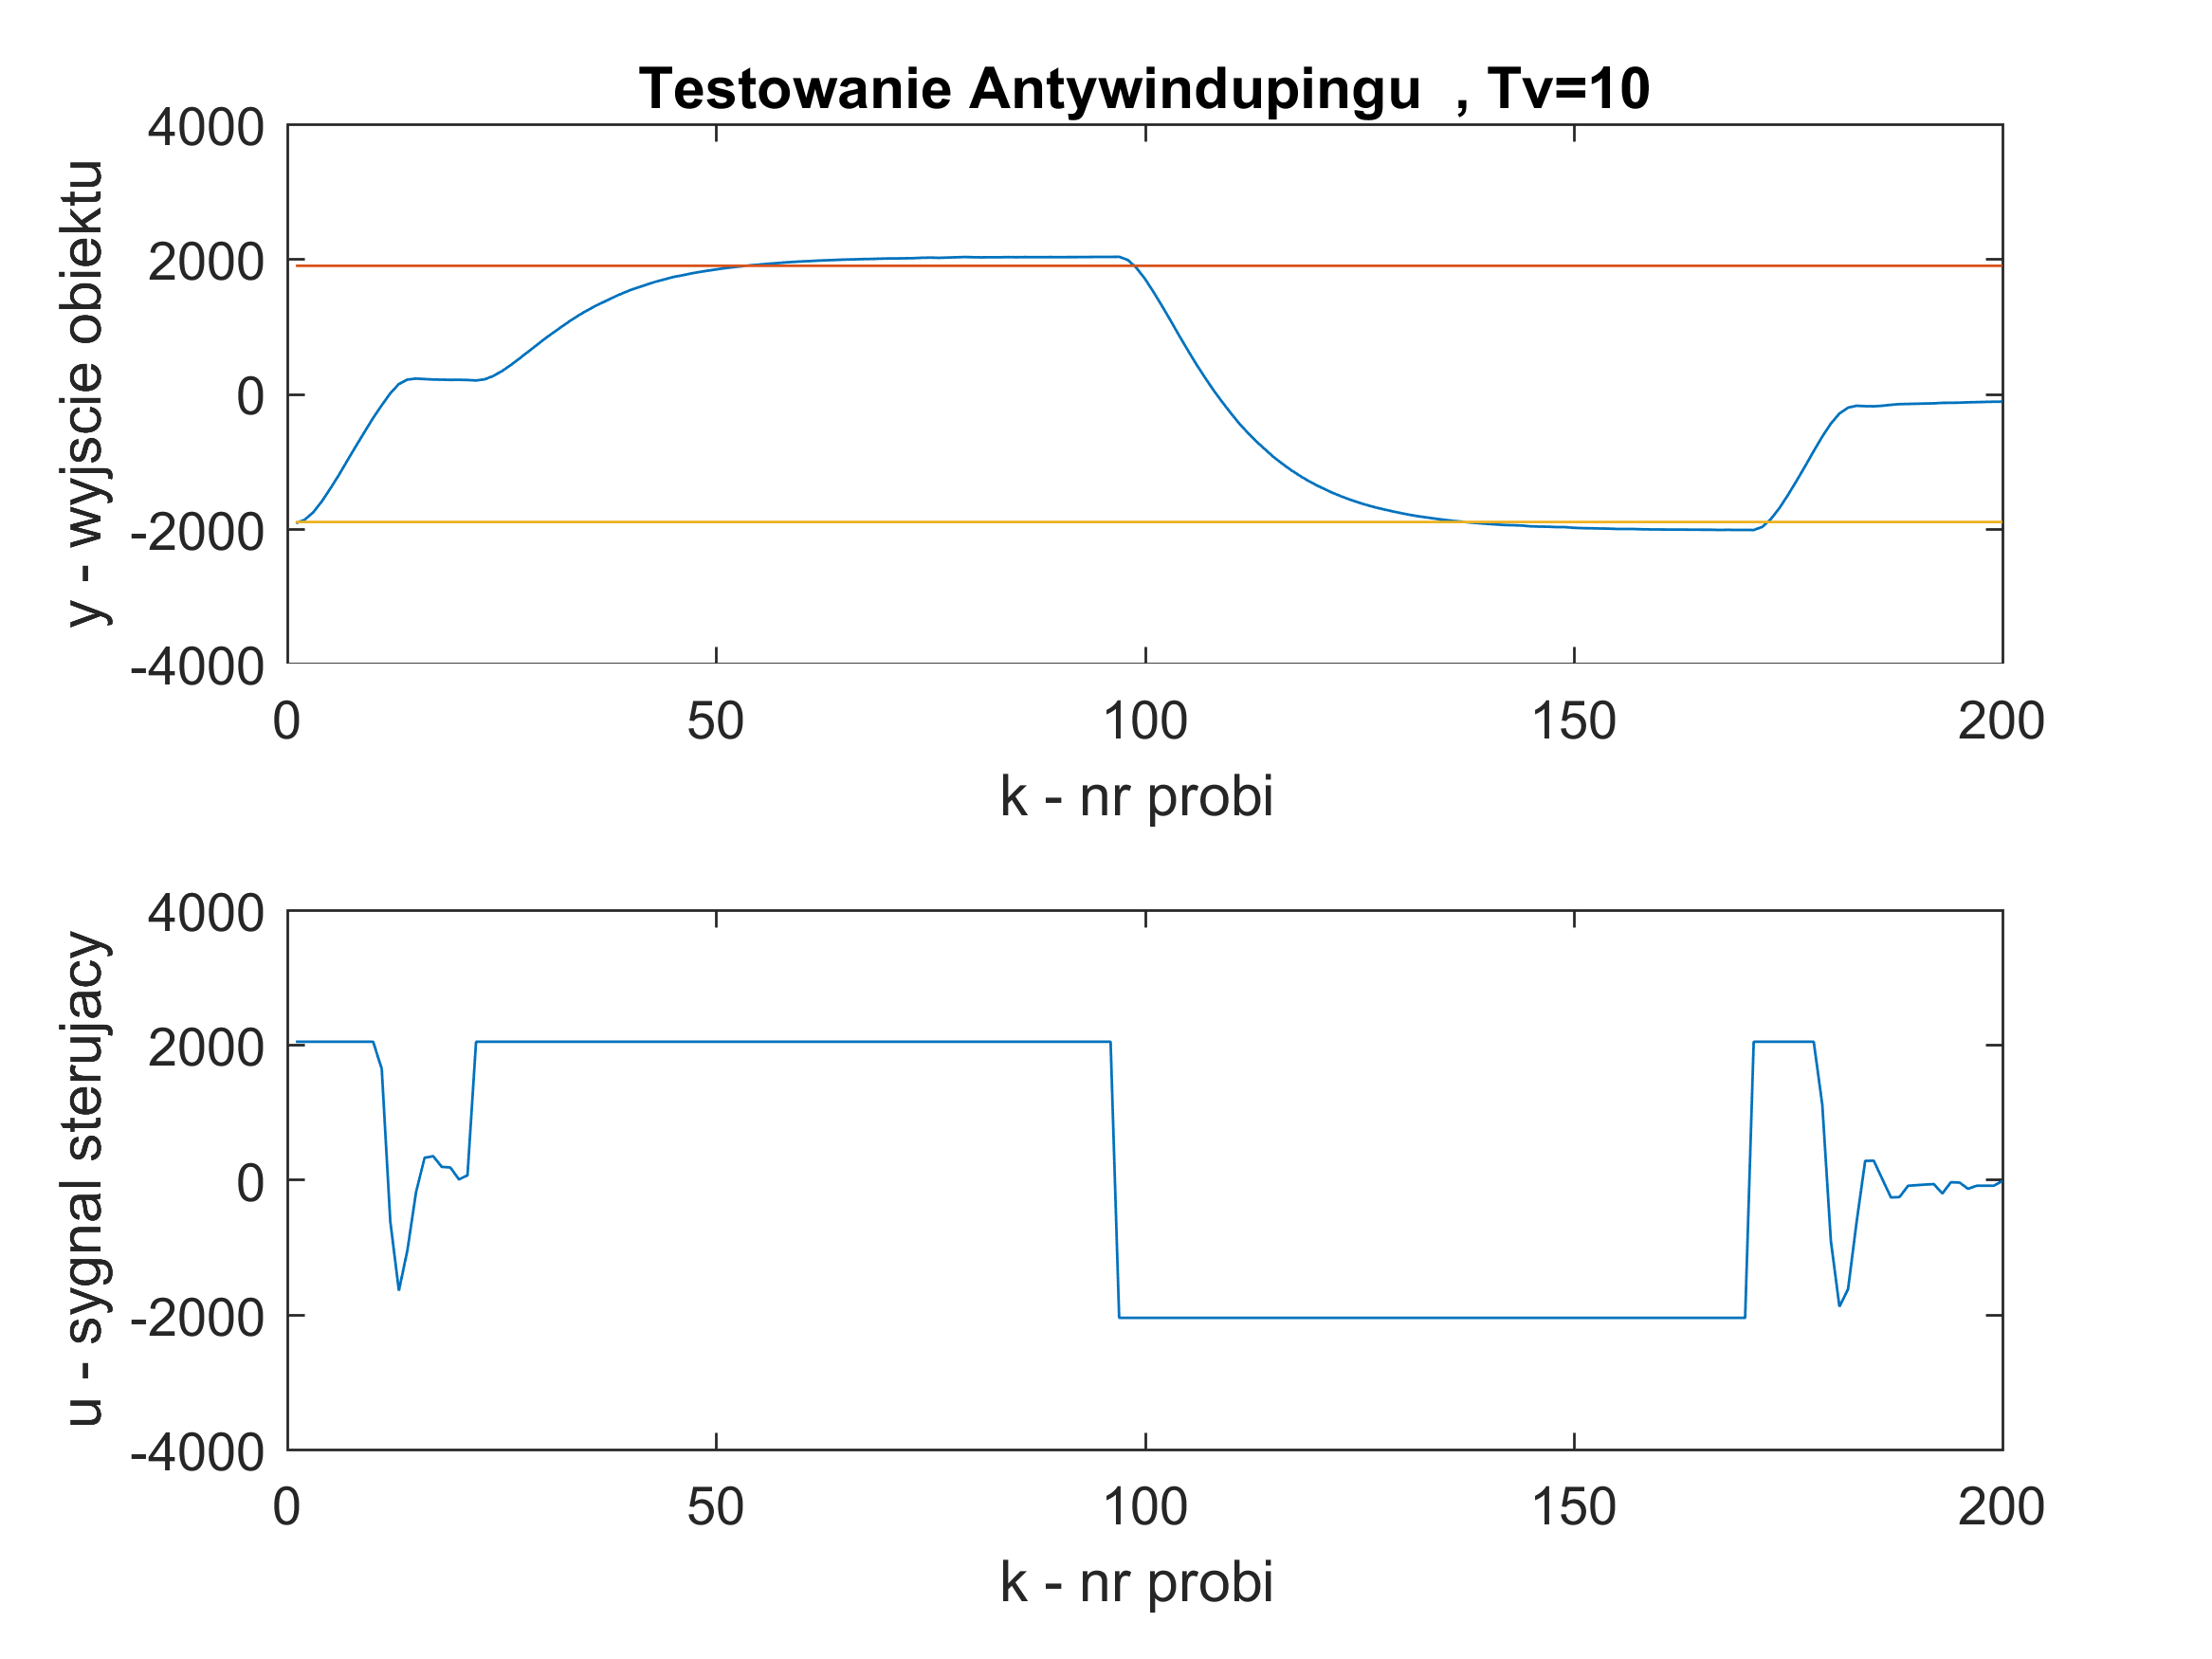
\includegraphics[width=0.9\linewidth]{aw10}
	\caption{Przebieg sygnałów przy $T_{v}=10$}
	\label{fig:aw10}
\end{figure}

\begin{figure}[H]
	\centering
	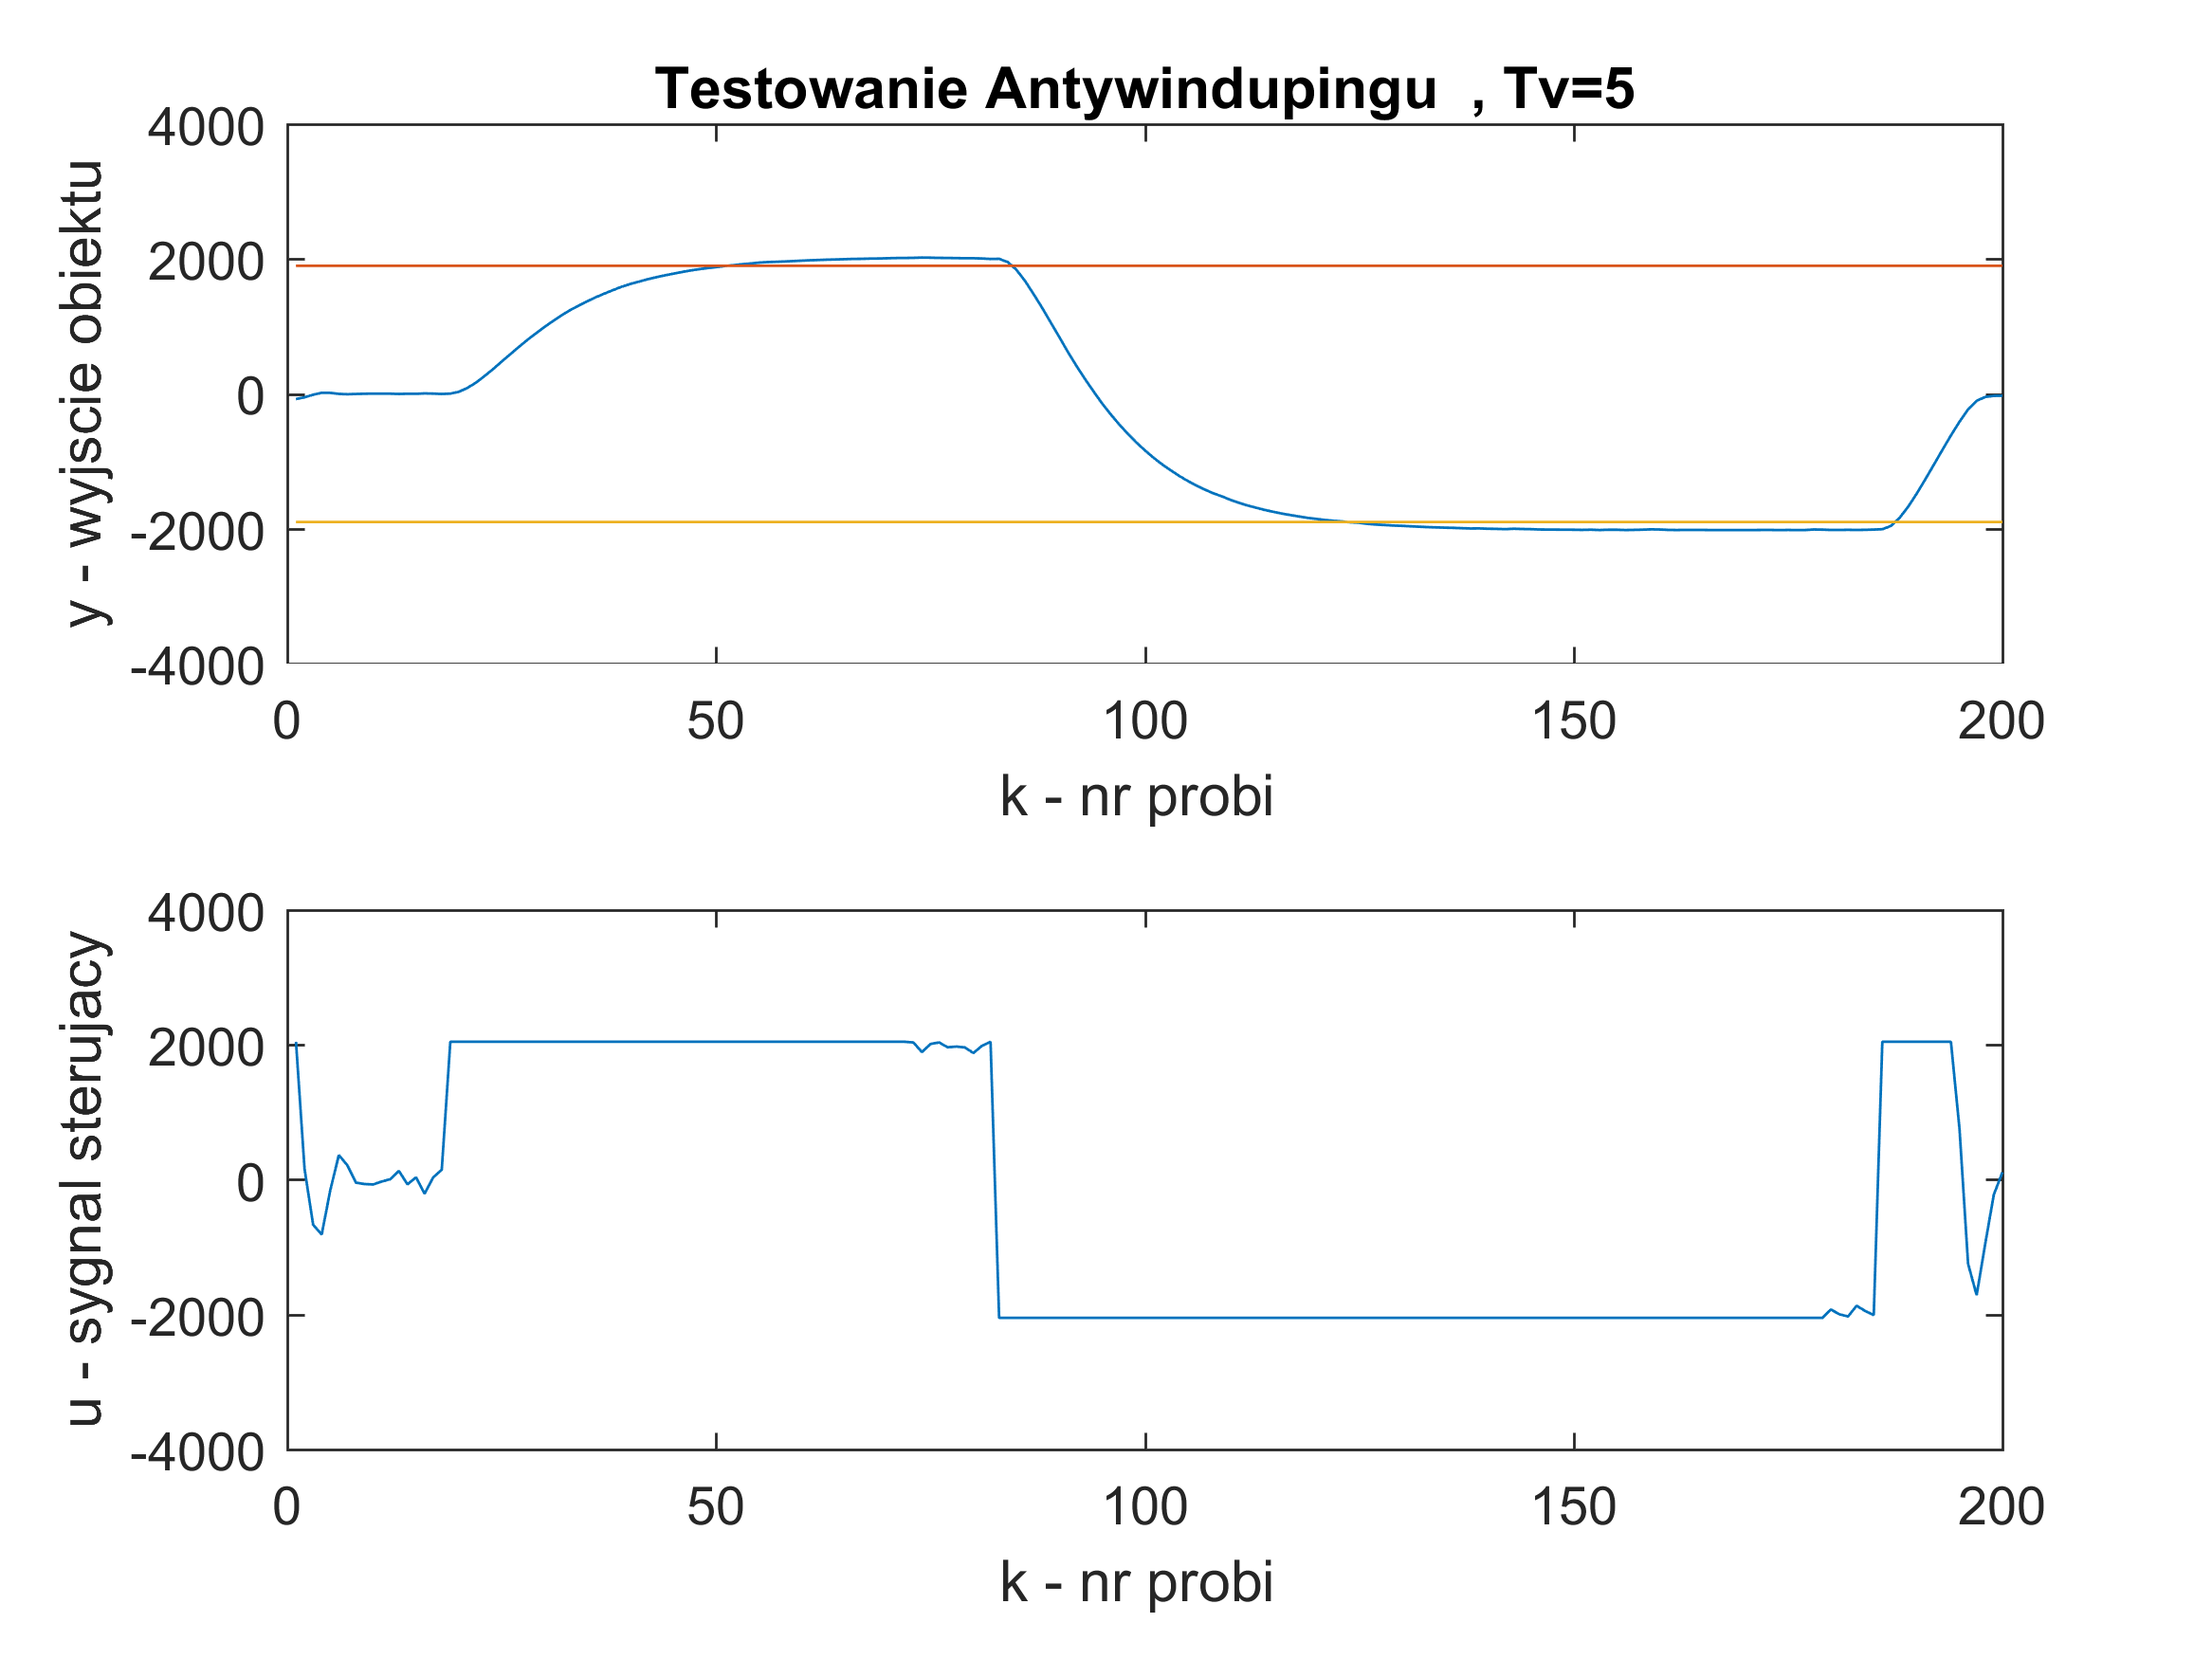
\includegraphics[width=0.9\linewidth]{aw5}
	\caption{Przebieg sygnałów przy $T_{v}=5$}
	\label{fig:aw5}
\end{figure}

\begin{figure}[H]
	\centering
	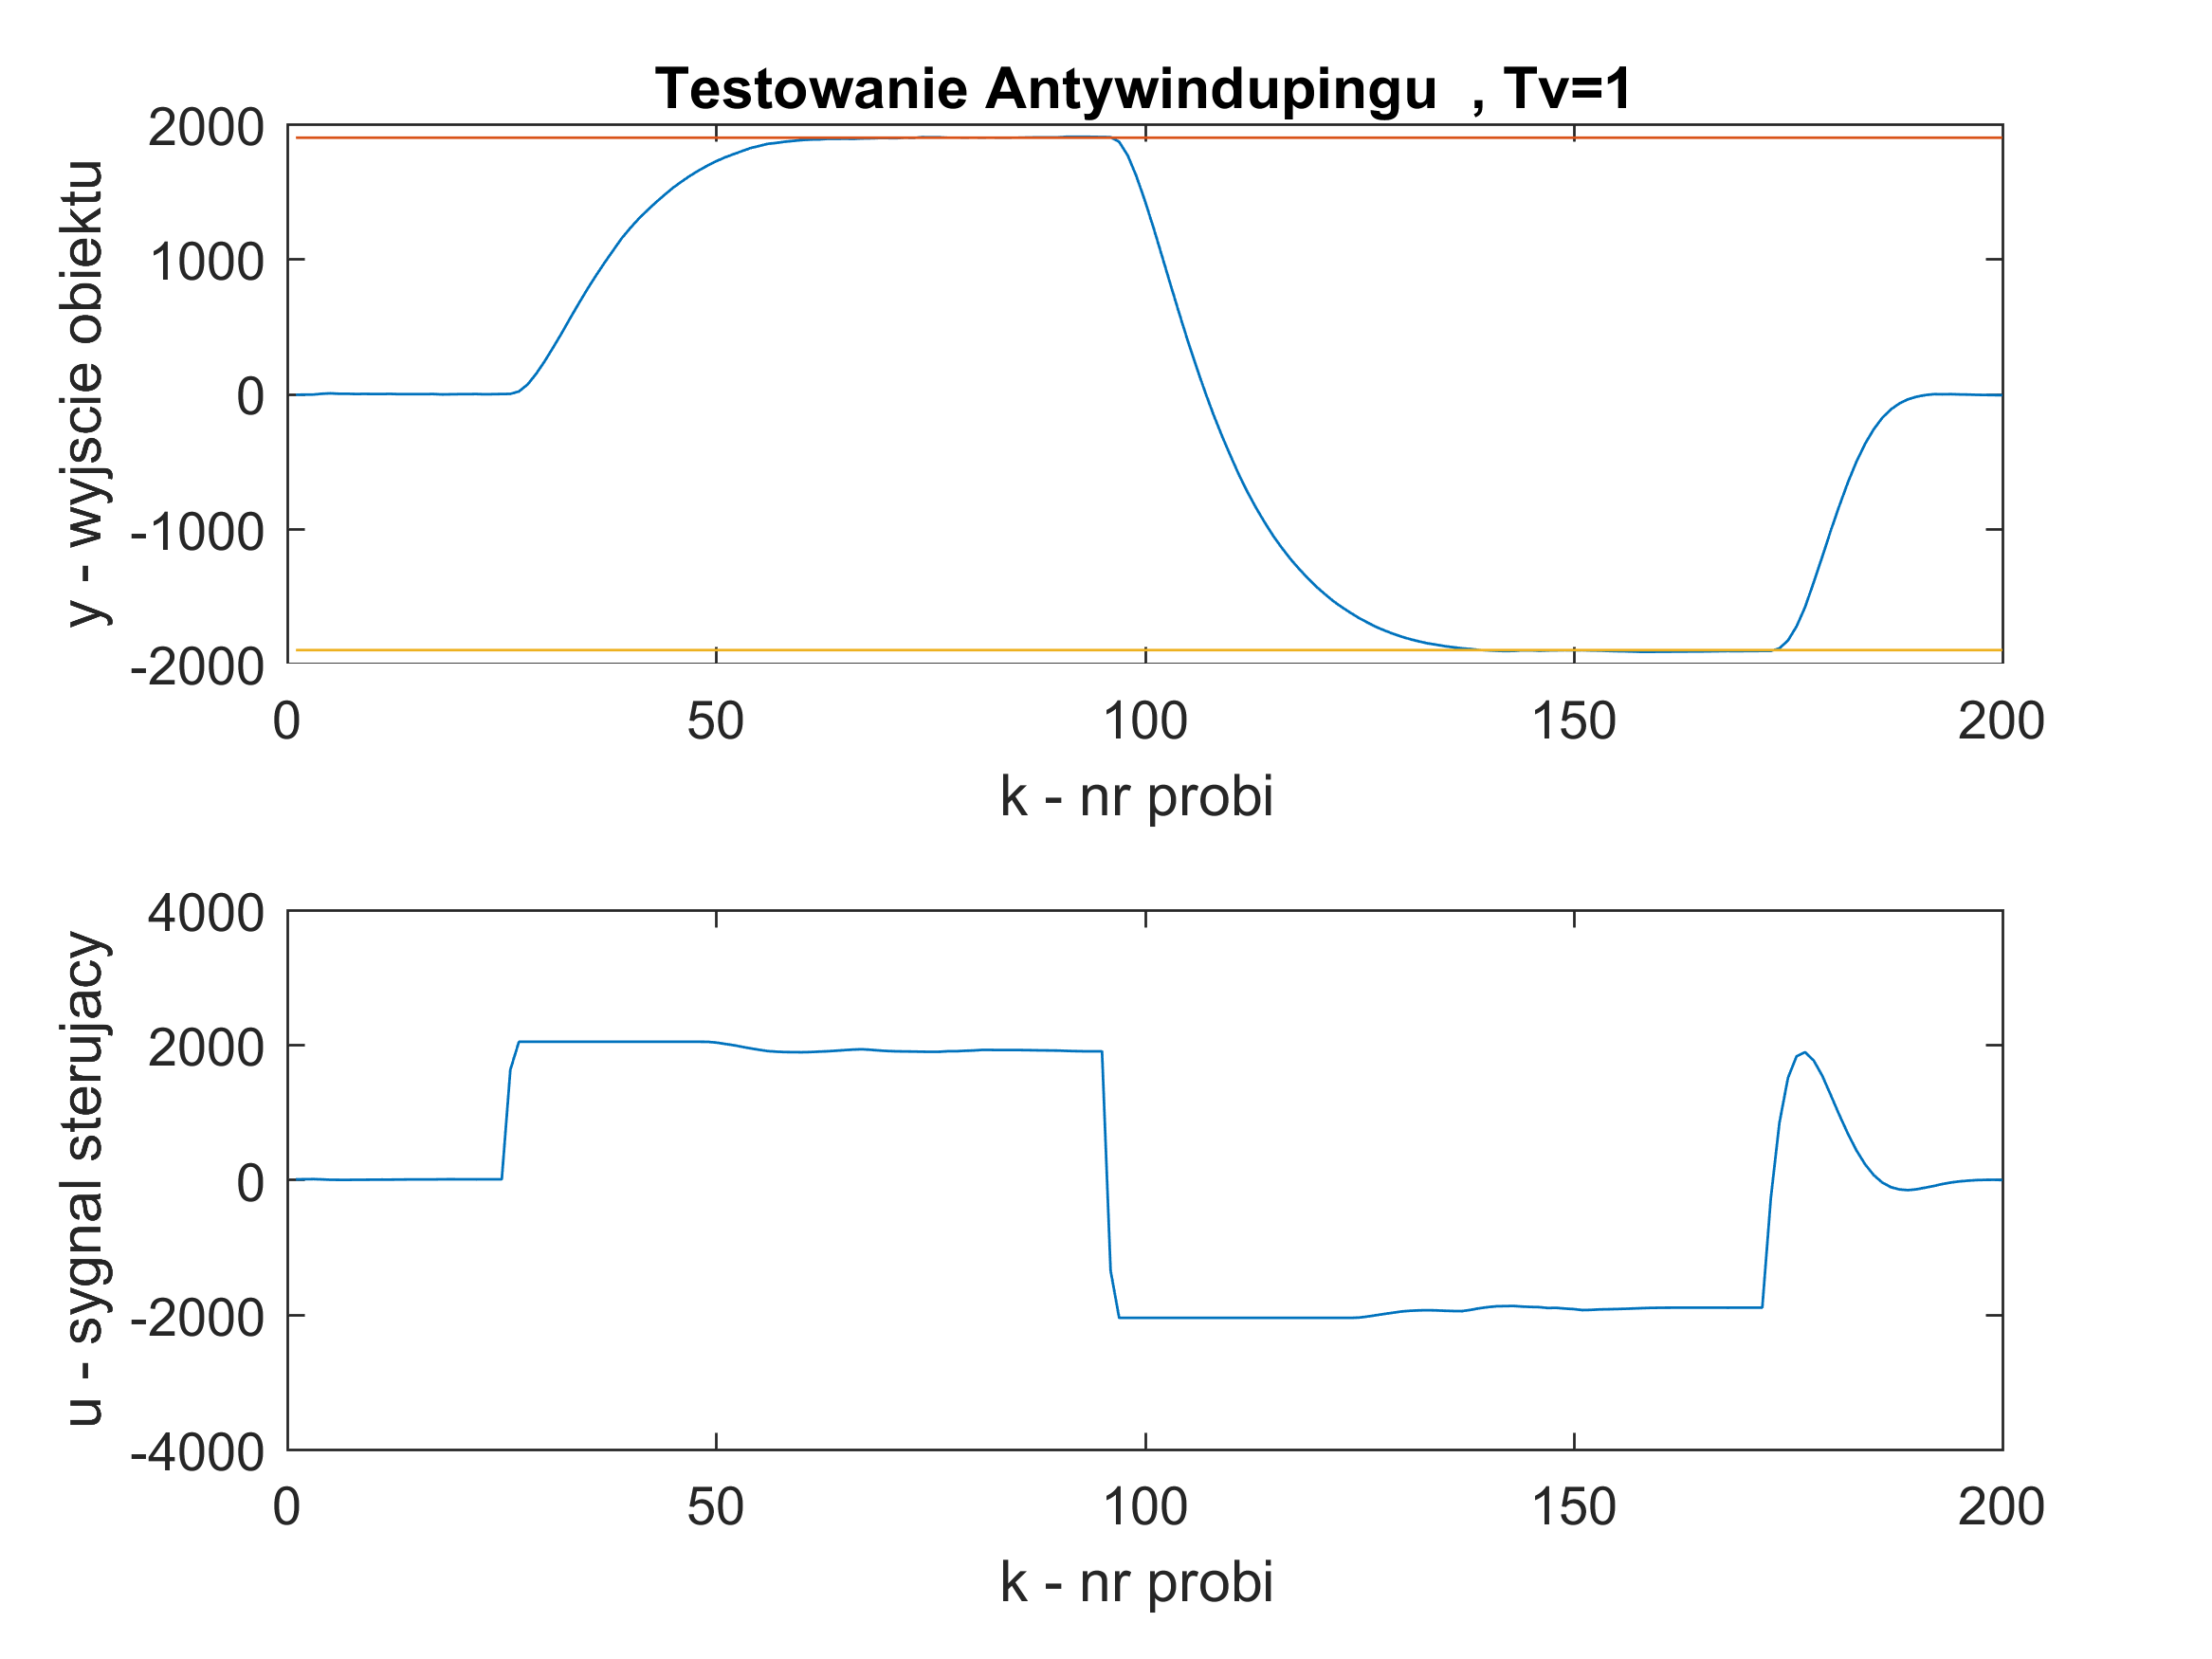
\includegraphics[width=0.9\linewidth]{aw1}
	\caption{Przebieg sygnałów przy $T_{v}=1$}
	\label{fig:aw1}
\end{figure}
Można zauważyć, że im mniejszy parametr $T_{v}$, a co za tym idzie większa wartość składowej sterowania $u_{I}$ odpowiadająca za anti-windup, tym mniejsze przeregulowanie i dzięki temu krótszy czas regulacji. Zauważmy, że regulator nie musi odcałkowywać. Przy przyjęciu $T_{v}=1$ udało się prawie całkowicie zredukować przeregulowanie. 
Z drugiej strony zbyt duże zmniejszenie parametru $T_{v}$ może spowodować, że obiekt zbyt wolno dochodzić będzie do wartości zadanej. Widać to na wykresie \ref{fig:aw11}, gdzie przy mniejszych zmianach wartości zadanej regulator nie jest w stanie w zadawalającym czasie osiągnąć zadanych wartości.
\begin{figure}[H]
	\centering
	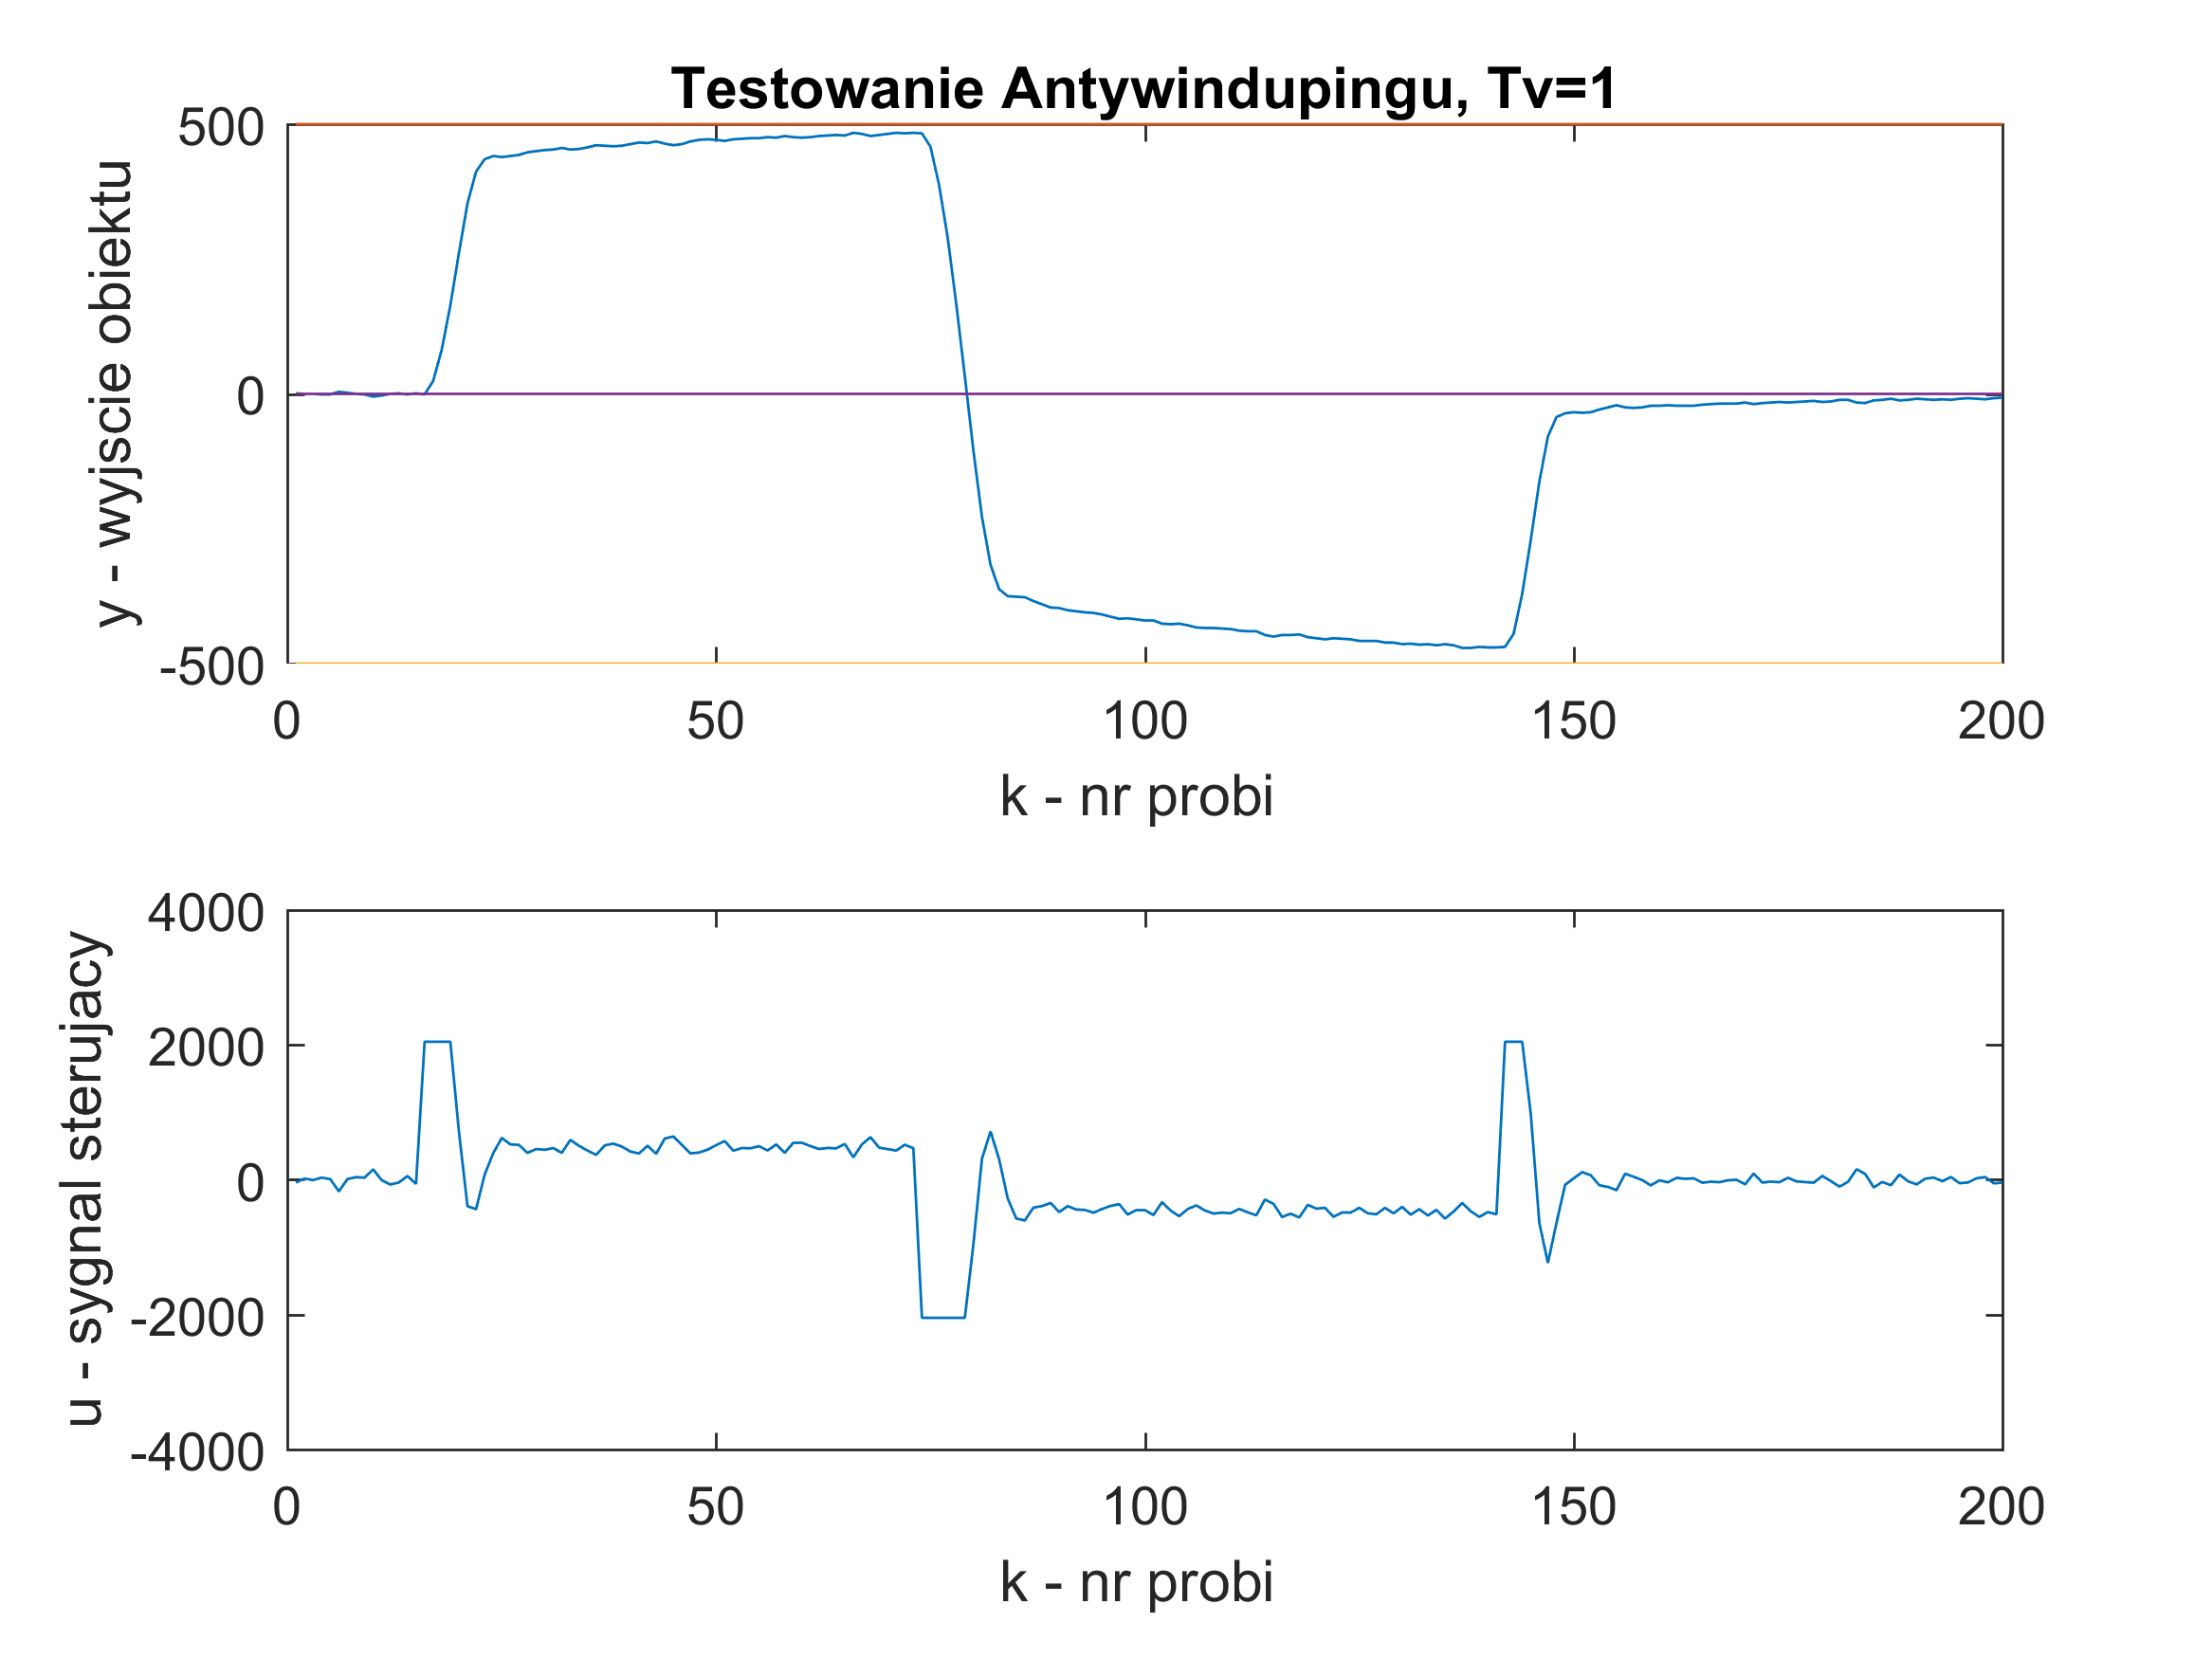
\includegraphics[width=0.9\linewidth]{aw11}
	\caption{Przebieg sygnałów przy $T_{v}=1$}
	\label{fig:aw11}
\end{figure}




\section{Algorytm DMC}

\subsection{Omówienie implementacji}
Druga część zadania polegała na zrealizowaniu regulatora za pomocą algorytmu DMC. Algorytm ten na podstawie modelu w postaci odpowiedzi skokowej oraz znajomości poprzednich sterowań generuje przyrosty sterowania na $N_{u}$ chwil do przodu. Parametr $N_{u}$ zwany jest horyzontem sterowania. Alogytm DMC wyznacza przyszłe zmiany sterowania tak, aby zminimalizować następujący wskaźnik jakości:
\[\min\limits_{\Delta U(k)} \{\sum_{p=1}^{N}(y^{zad}(k+p|k)-\widehat{y}(k+p|k))^2+\sum_{p=0}^{N_{u}-1}\lambda_{p}(\Delta u(k+p|k))^2 \} ,\]				
gdzie $y^{zad}(k+p|k)$ jest wartością zadaną w chwili $k+p$ wyznaczoną w chwili $k$, $\widehat{y}(k+p|k)$ jest przwidywaną wartością wyjścia obiektu w chwili $k+p$ wyznaczoną w chwili $k$, $\lambda_{p}$ jest parametrem regulatora określającym karę za zmiany sygnału sterującego, a $\Delta u(k+p|k)$ jest przyrostem sterowania w chwili $k+p$ obliczonym w chwili k. \\
Jako, że w każdej iteracji interesuje nas obliczenie tylko $\Delta u(k|k)$ prawo regulacji można opisać następującym wzorem:
\[u(k|k)=u(k-1)+K_{e}e(k)-K_{u}\Delta U^{P}(k),\]
gdzie $u(k-1)$ oznacza wartość sterowania w poprzedniej chwili czasu, $e(k)$ oznacza aktualny uchyb, a wektor $\Delta U^{P}(k)$ zawiera $D-1$ poprzednich przyrostów sygnału sterującego.\\
Składowe $K_{u}$ i $K_{e}$ bezpośrednio pochodzą z macierzy $K$, którą można opisać następującym wzorem:
\[K = 
\begin{bmatrix}
M^{T}M+\lambda I 
\end{bmatrix} ^{-1}M^{T} = 
\begin{bmatrix}
\overline{K}_1 \\\overline{K}_2 \\ \vdots\\ \overline{K}_{N_{u}}
\end{bmatrix} = 
\begin{bmatrix}
K_{1,1} & K_{1,2} & \dots & K_{1,N} \\
K_{2,1} & K_{2,2}  & \dots & K_{2,N} \\
\vdots  & \vdots &\ddots  &\vdots \\
K_{N_{u},1}   & K_{N_{u},2}  &\dots  & K_{N_{u},N}
\end{bmatrix}
\]
\[K_e = \sum_{i=1}^{N}K_{1,i} \]

\[ K_u = \overline{K}_1 M^{P} \]

Macierze $M$ i $M^{P}$ składają się z elementów odpowiedzi skokowej, więc macierz $K$ wystarczy obliczyć raz offline, i w kolejnych iteracjach regulatora wystarczy korzystać z obliczonego wektora $K_{u}$ i stałej $K_{e}$.
\[M = 
\begin{bmatrix}
s_{1} & 0 & \dots & 0 \\
s_{2} & s_{1}  & \dots & 0 \\
\vdots  & \vdots &\ddots  &\vdots \\
s_{N}   & s_{N-1} &\dots  & s_{N-N_{u}+1}
\end{bmatrix} 
M^{P} = 
\begin{bmatrix}
s_{2}-s_{1} &  \dots & s_{D}-s_{D-1} \\
s_{3}-s_{1} &\dots & s_{D+1}-s_{D-1} \\
\vdots &\ddots &\vdots \\
s_{N+1}-s_{1}   &\dots  & s_{N+D-1}-s_{D-1}
\end{bmatrix} 	
\]	


W celu implementacji regulatoa DMC należało wyznaczyć znormalizowaną odpowiedź skokową. Zebrana została odpowiedź obiektu na skok sterownania, a następnie od otrzymanych wartości została odjęta wartość z pierwszej chwili czasu. Na koniec wartości zostały podzielone przez wartość skoku sterowania. 

\begin{figure}[H]
	\centering
	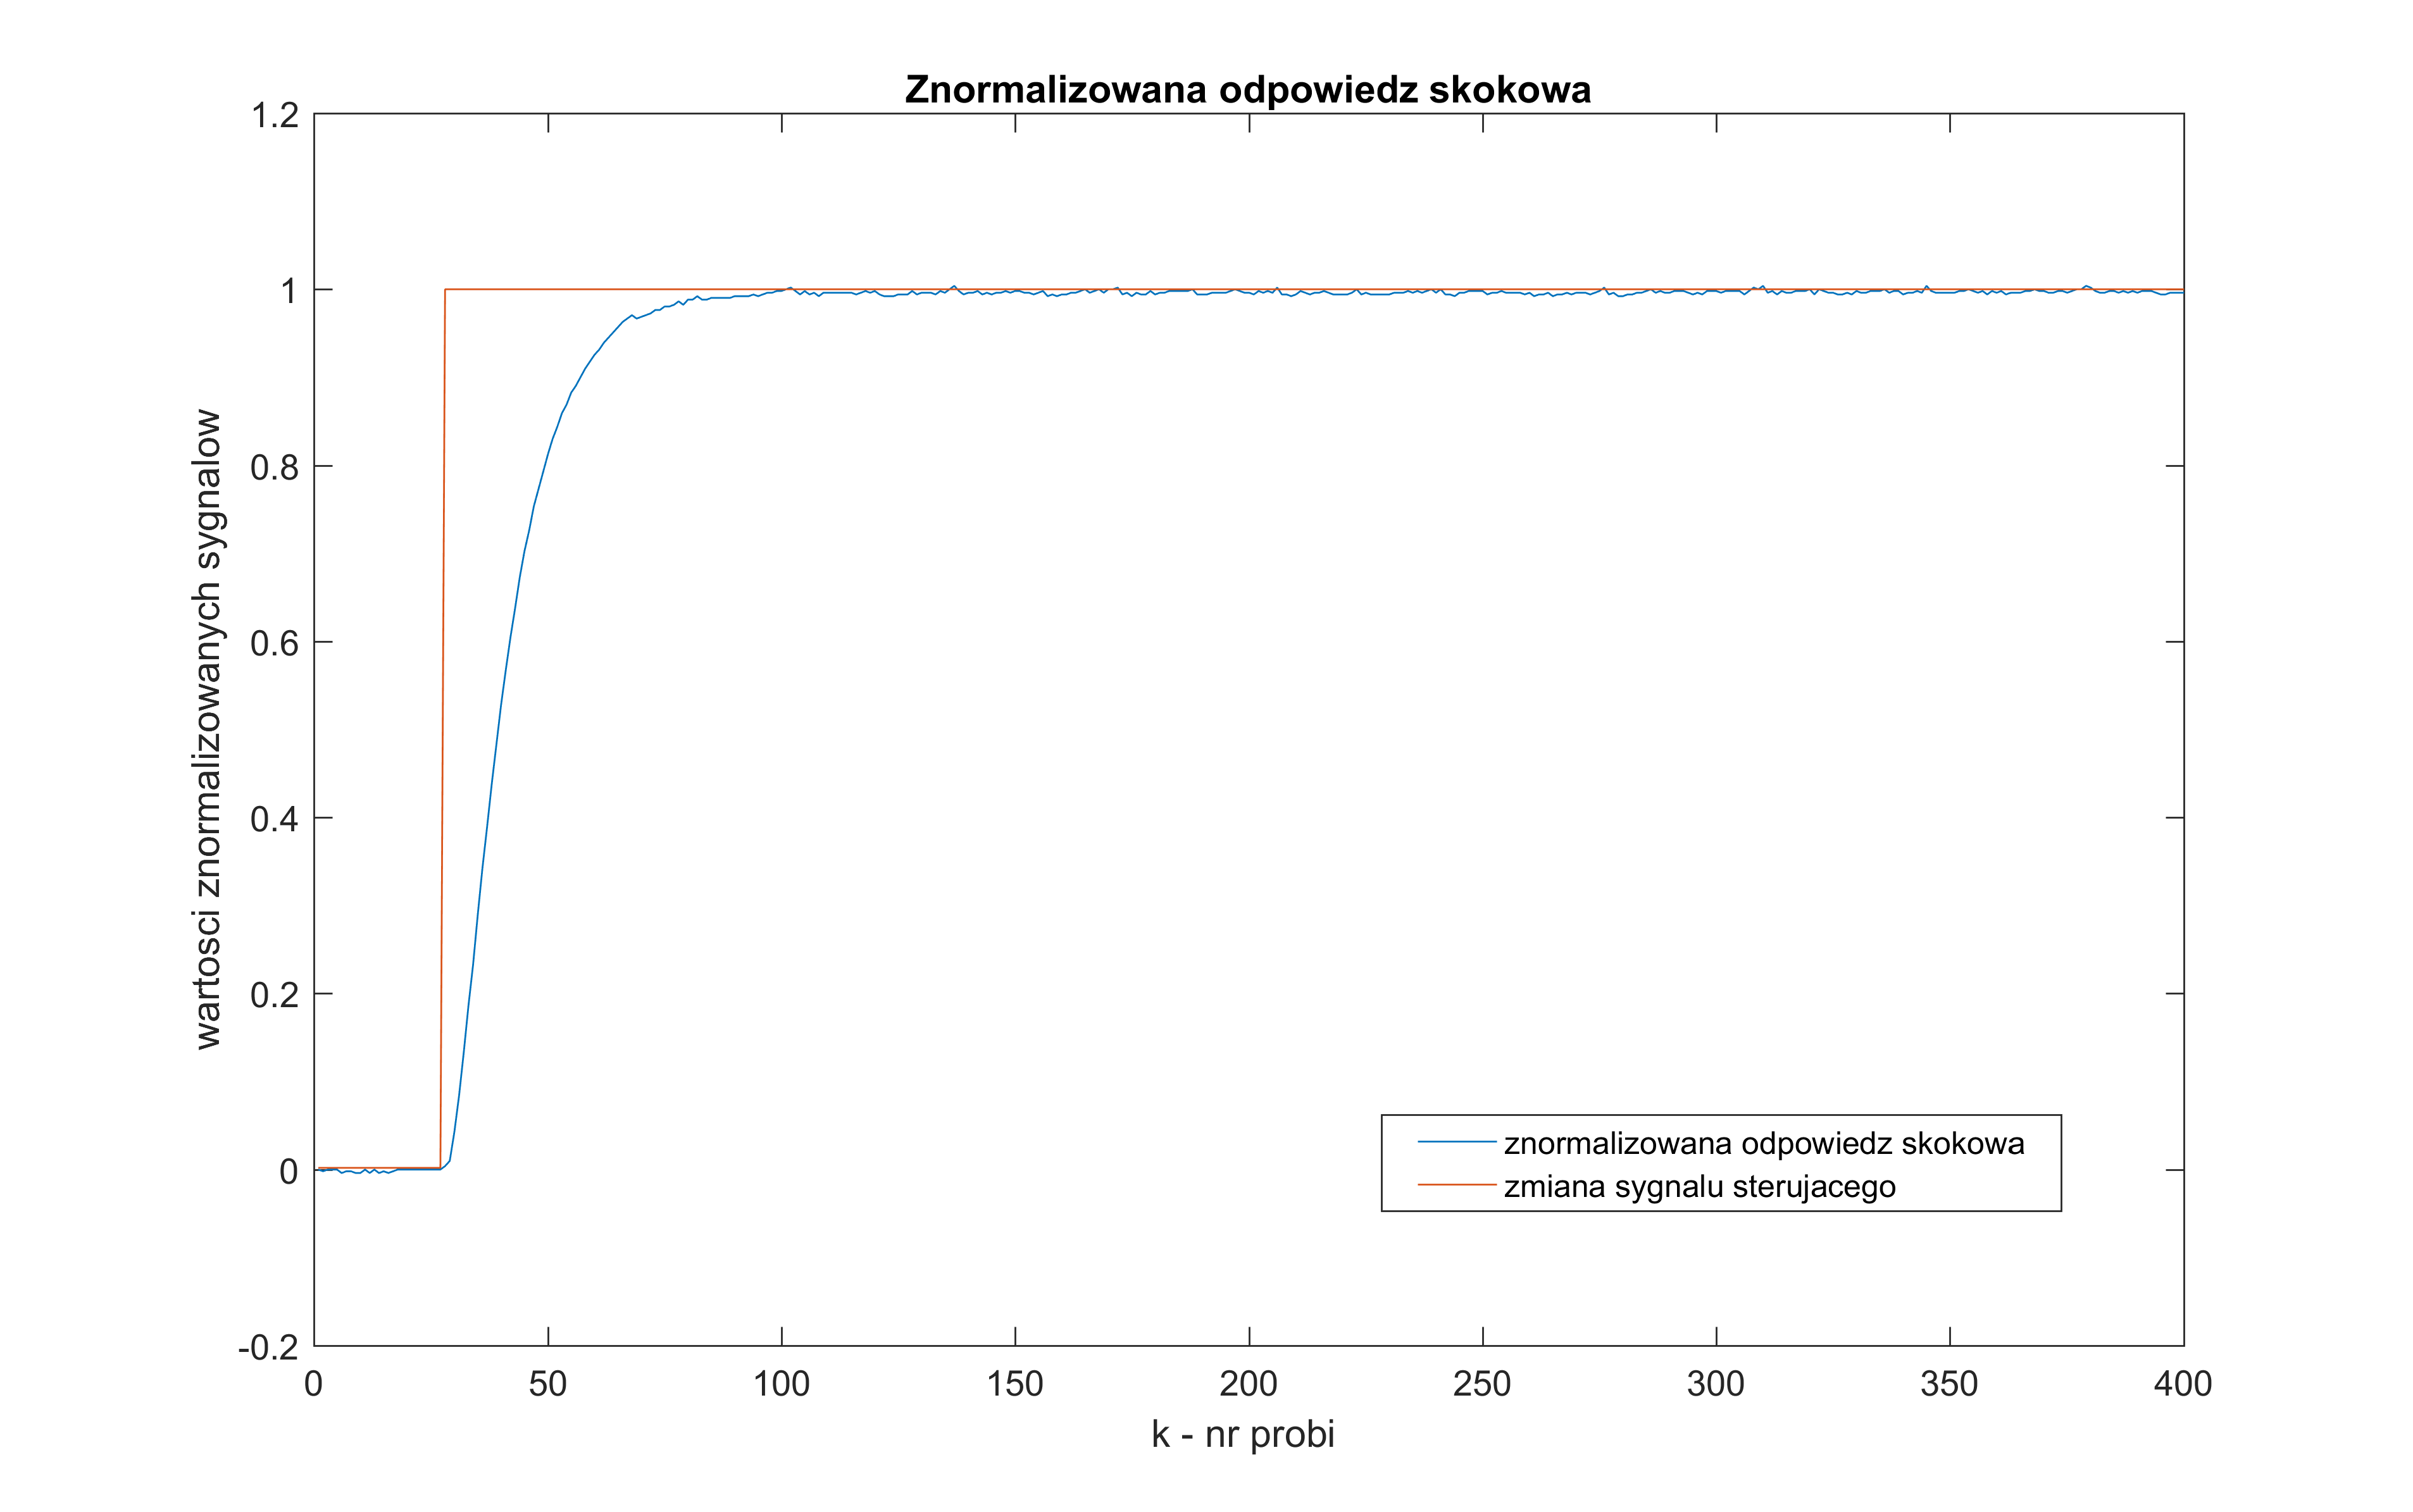
\includegraphics[width=0.9\linewidth]{odp_skok_wykre}
	\caption{Znormalizowana odpowiedź skokowa}
	\label{fig:odp_skok_wykre}
\end{figure}

Przyjęłyśmy horyzont dynamiki obiektu równy: $D=60$, ponieważ po 60 próbkach od momentu zmiany sterowania, wyjście obiektu stabilizowało się - nie zmieniało znacząco swojej wartości.
Parametrami, jakimi stroi się regulator DMC są:\\
- $N$ - horyzont predykcji,\\
- $N_{u}$ - horyzont sterowania,\\
- $\lambda$ - parametr kary za zmieny sygnału sterującego.\\
W celu obliczenia wektora $K_{u}$ i elementu $K_{e}$ napisany został skrypt w \textit{Matlabie}.  Skrypt ten składał się z kilku etapów:\\
- zdefiniowanie parametrów regulatora,\\
- generacja macierzy $M$ i $M^{P}$, \\
- obliczenie macierzy $K$ zgodnie z podanym powyżej wzorem,\\
- obliczenie wartości $K_{e}$ oraz wektora $K_{u}$.\\
Regulator zrealizowany na mikrokontrolerze wykorzystuje obliczone w \textit{Matlabie} wartości $K_{e}$ i $K_{u}$. Na mikrokontrolerze przyjęte zostały oznaczenia $Ke=K_{e}$, $Kuu=K_{u}$ $dup=\Delta U^{P}$.\\
Algorytm regulacji na mikrokontrolerze składa się z następujących etapów:\\
- zebranie wartrości wyjścia,\\
- obliczenie uchybu,\\
- obliczenie fragmentu przyrostu sterowania (fragment $K_{u} \cdot \Delta U^{P}$ )\\
- obliczenie przyrostu sterowania ($\Delta u(k|k)= K_{e} \cdot e(k) - K_{u} \cdot \Delta U^{P}$ ), \\
- obliczenie wartości sterowania, \\
- sprawdzenie, czy wartość sygnału sterującego nie przekracza ograniczeń, \\
- zapamiętanie wartości sygnału sterującego, \\
- przesunięcie wektora $dup$ i umieszczenie na pierwszym miejscu aktualnie obliczonego przyrostu sygnału sterującego,\\
- wysłanie sterowania.

\begin{lstlisting} [caption={Kod realizujący regulator DMC}]
static float y = 0.0f;
static float u = 0.0f;
//zebranie wartosci wyjscia
y = (input-2048.0f);

//wyznaczenie uchybu
e = y_zad - y; 

//obliczanie przyrostu sterowania dla aktualnej iteracji
for (i = 0; i < wymiar; ++i){
sum = sum+dup[i]*Kuu[i];
}
delta_u = Ke*e-sum;

//obliczenie wartosci sygnalu sterujacego jako suma poprzedniego sterowania i przyrostu sterowania
u = upoprz+delta_u;

//wyznaczenie ograniczenia sygnalu sterujacego
if(u >  2047.0f) u =  2047.0f;
if(u < -2048.0f) u = -2048.0f;

//wyznaczenie wartosci sterowania i przyrostu sterowania po zastosowaniu ograniczen
delta_u = u-upoprz;
upoprz = u;

// usuniecie najstarszego elementu z wektora
for (i = wymiar-1; i > 0; --i){
dup[i] = dup[i-1];
}

//dolozenie delty z aktualnej iteracji na poczatek wektora dup
dup[0] = delta_u; 

//wyslanie sterowania
output = u+2048.0f; 
updateControlSignalValue(output);
\end{lstlisting}

\subsection{Wyznaczanie horyzontu predykcji}
Pierwszym krokiem dostrajania regulatora DMC jest ustalenie horyzontu predykcji. Ogólnie przyjętą zasadą jest przyjęcie w tym kroku horyzontu sterowania równego horyzontowi predykcji $N_{u}=N$ oraz $\lambda=1$. Eksperymenty wykonuje się zaczynając od $N=D$ i stopniowo zmniejsza się ten parametr do momentu, w którym w widoczny sposób pogorszyła się trajektoria sygnału wyjściowego. 
\begin{figure}[H]
	\centering
	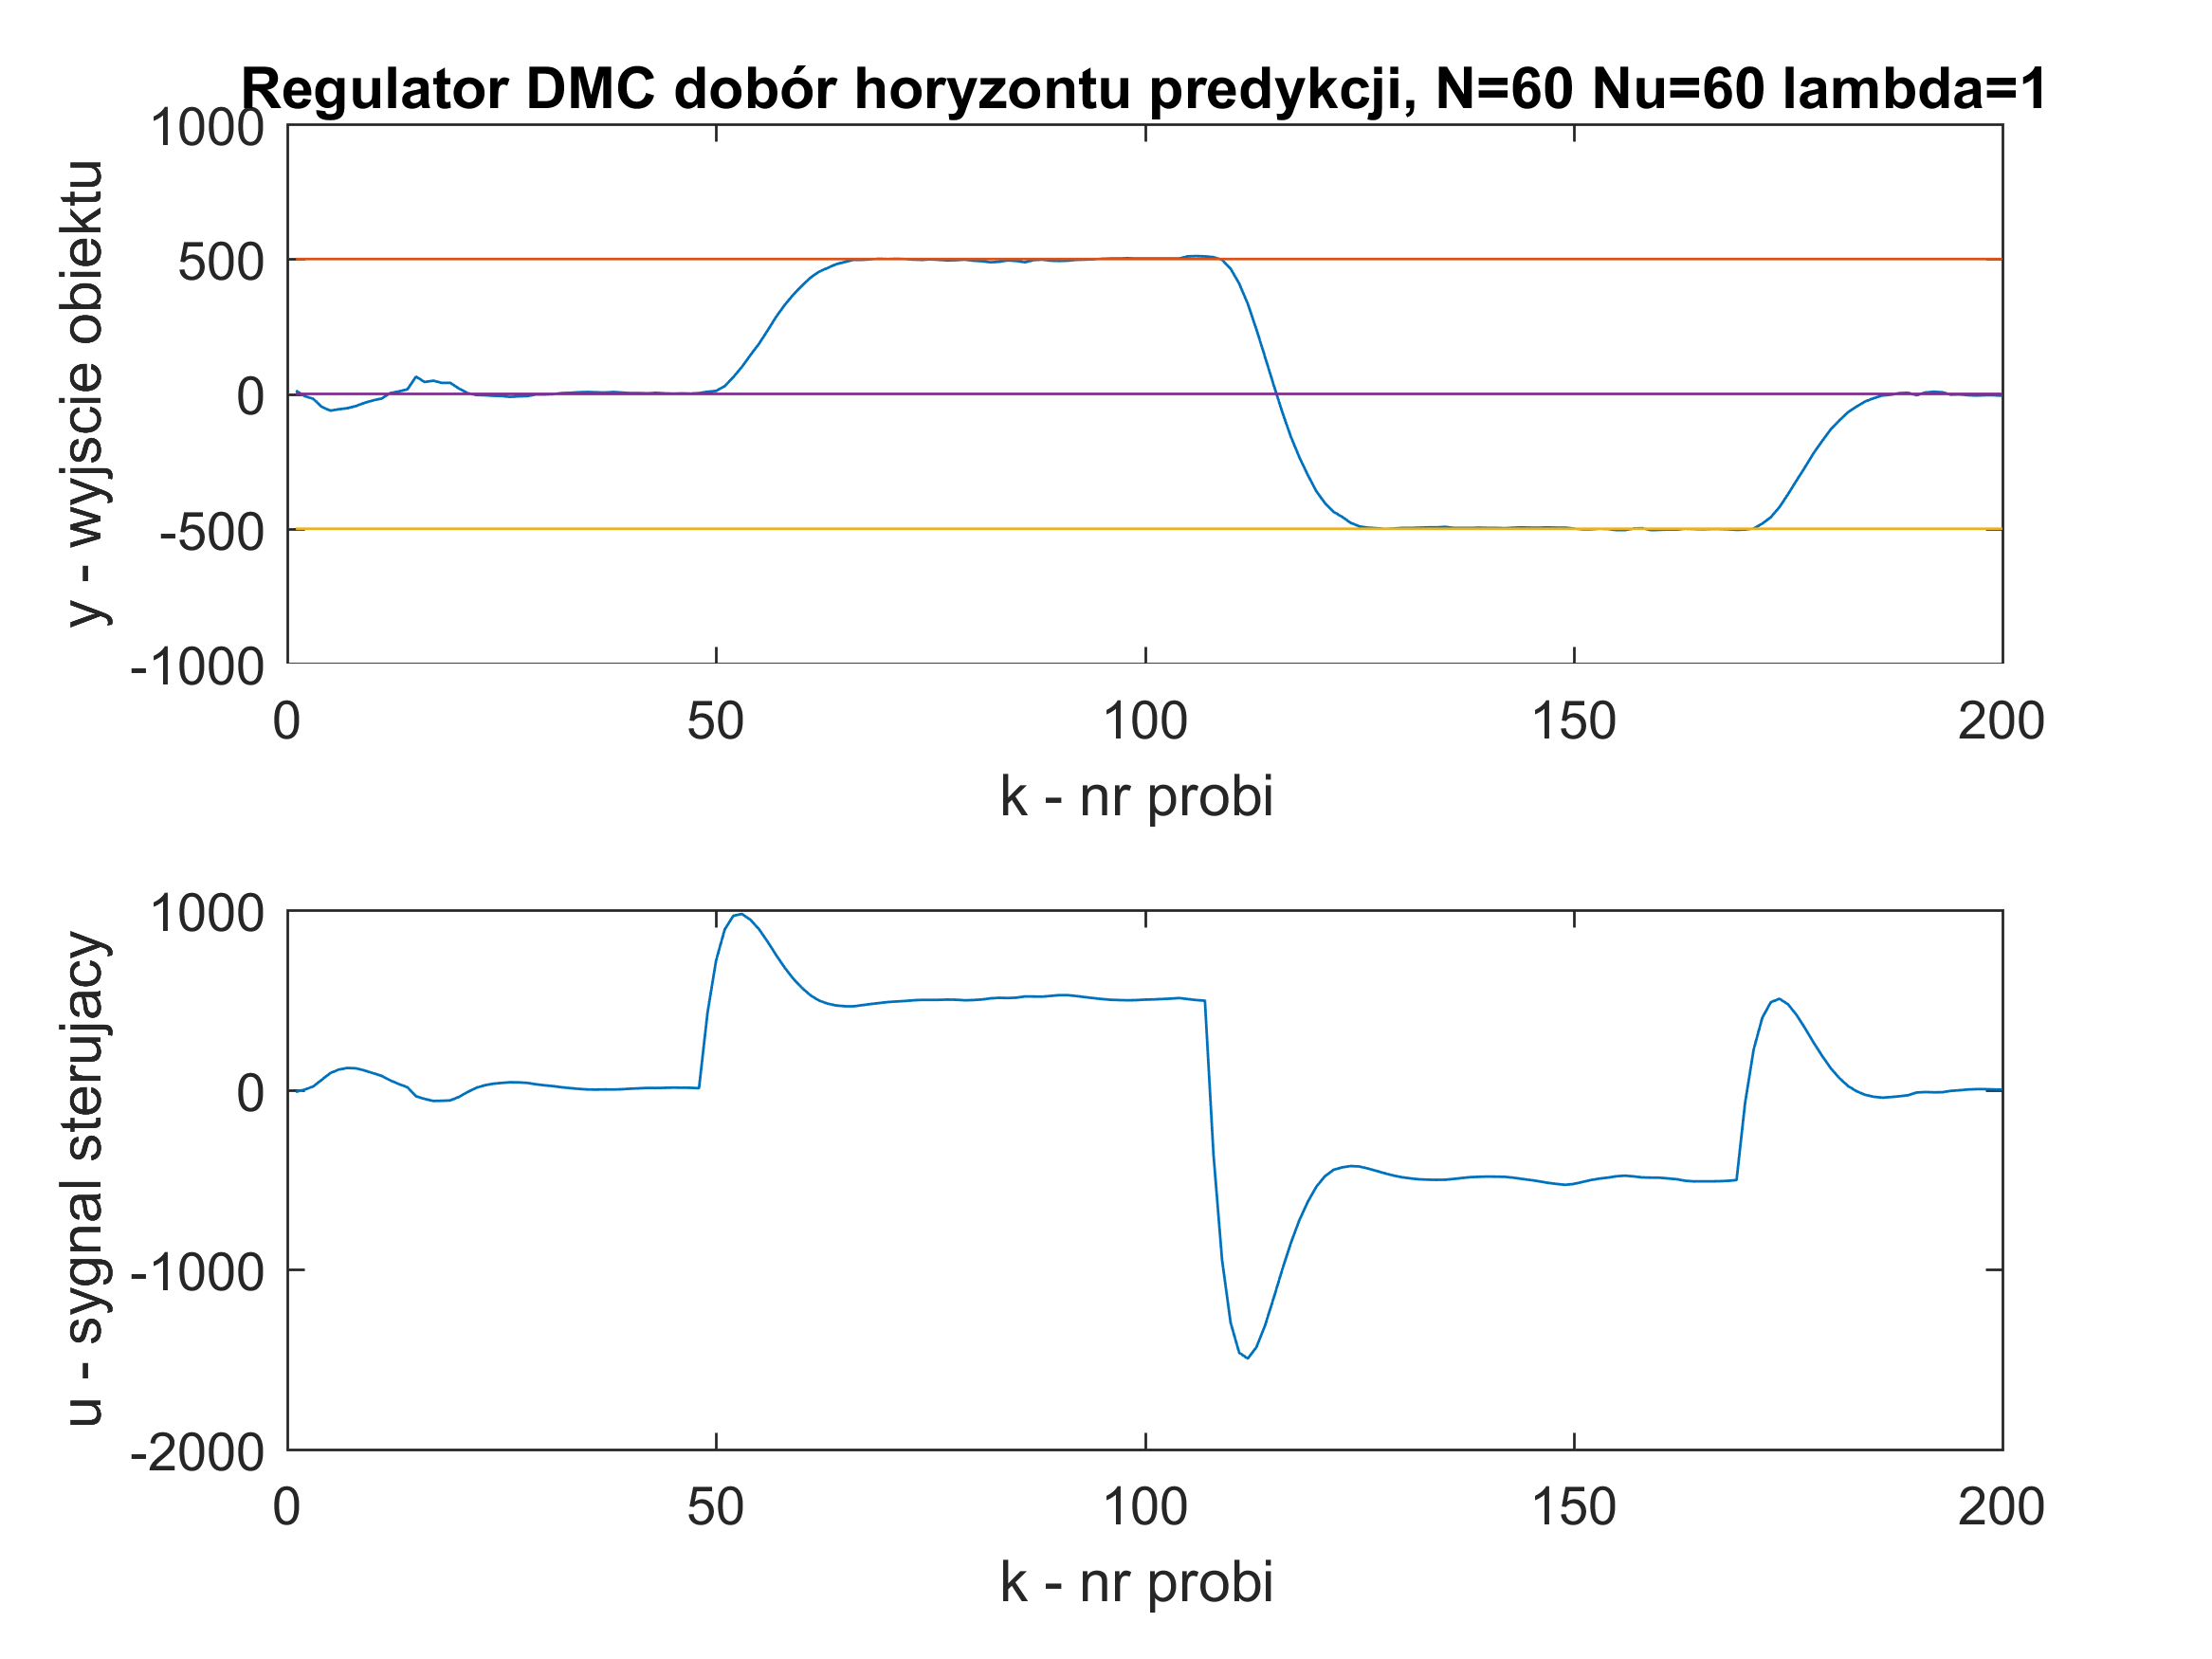
\includegraphics[width=0.9\linewidth]{DMC60601}
	\caption{Przebieg sygnałów przy $N=60$}
	\label{fig:DMC60601}
\end{figure}
\begin{figure}[H]
	\centering
	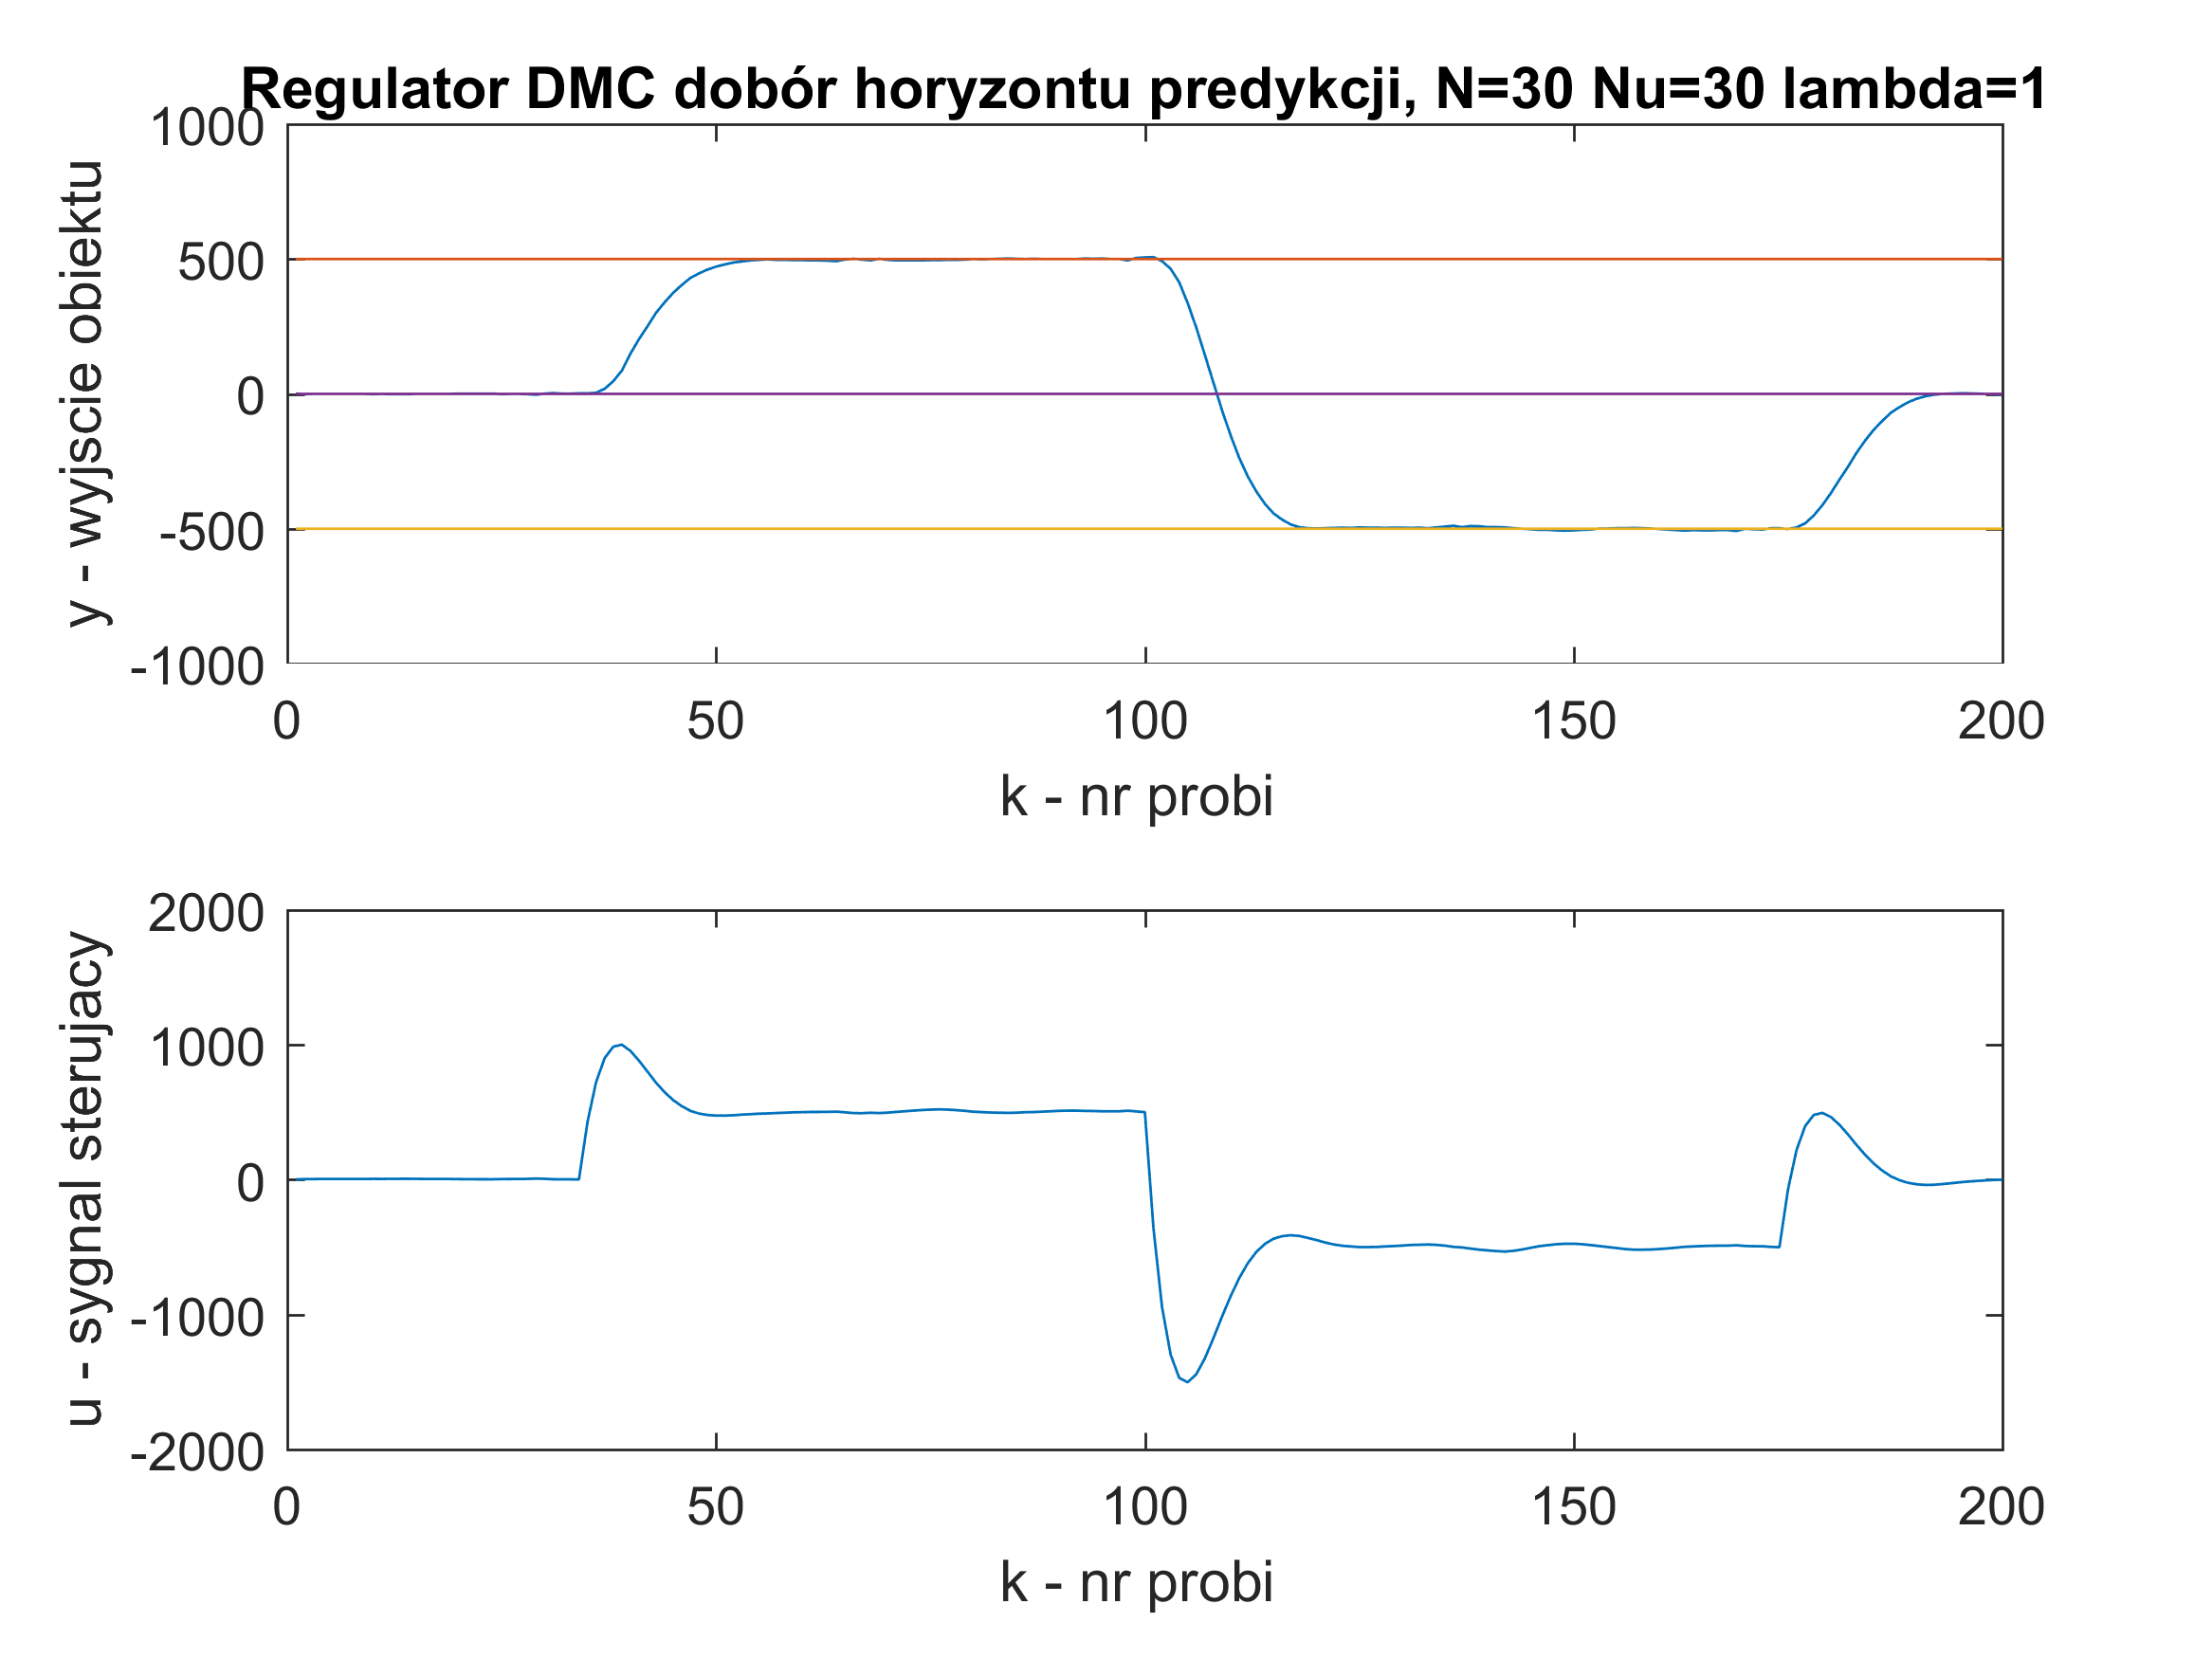
\includegraphics[width=0.9\linewidth]{DMC30301}
	\caption{Przebieg sygnałów przy $N=30$}
	\label{fig:DMC30301}
\end{figure}
\begin{figure}[H]
	\centering
	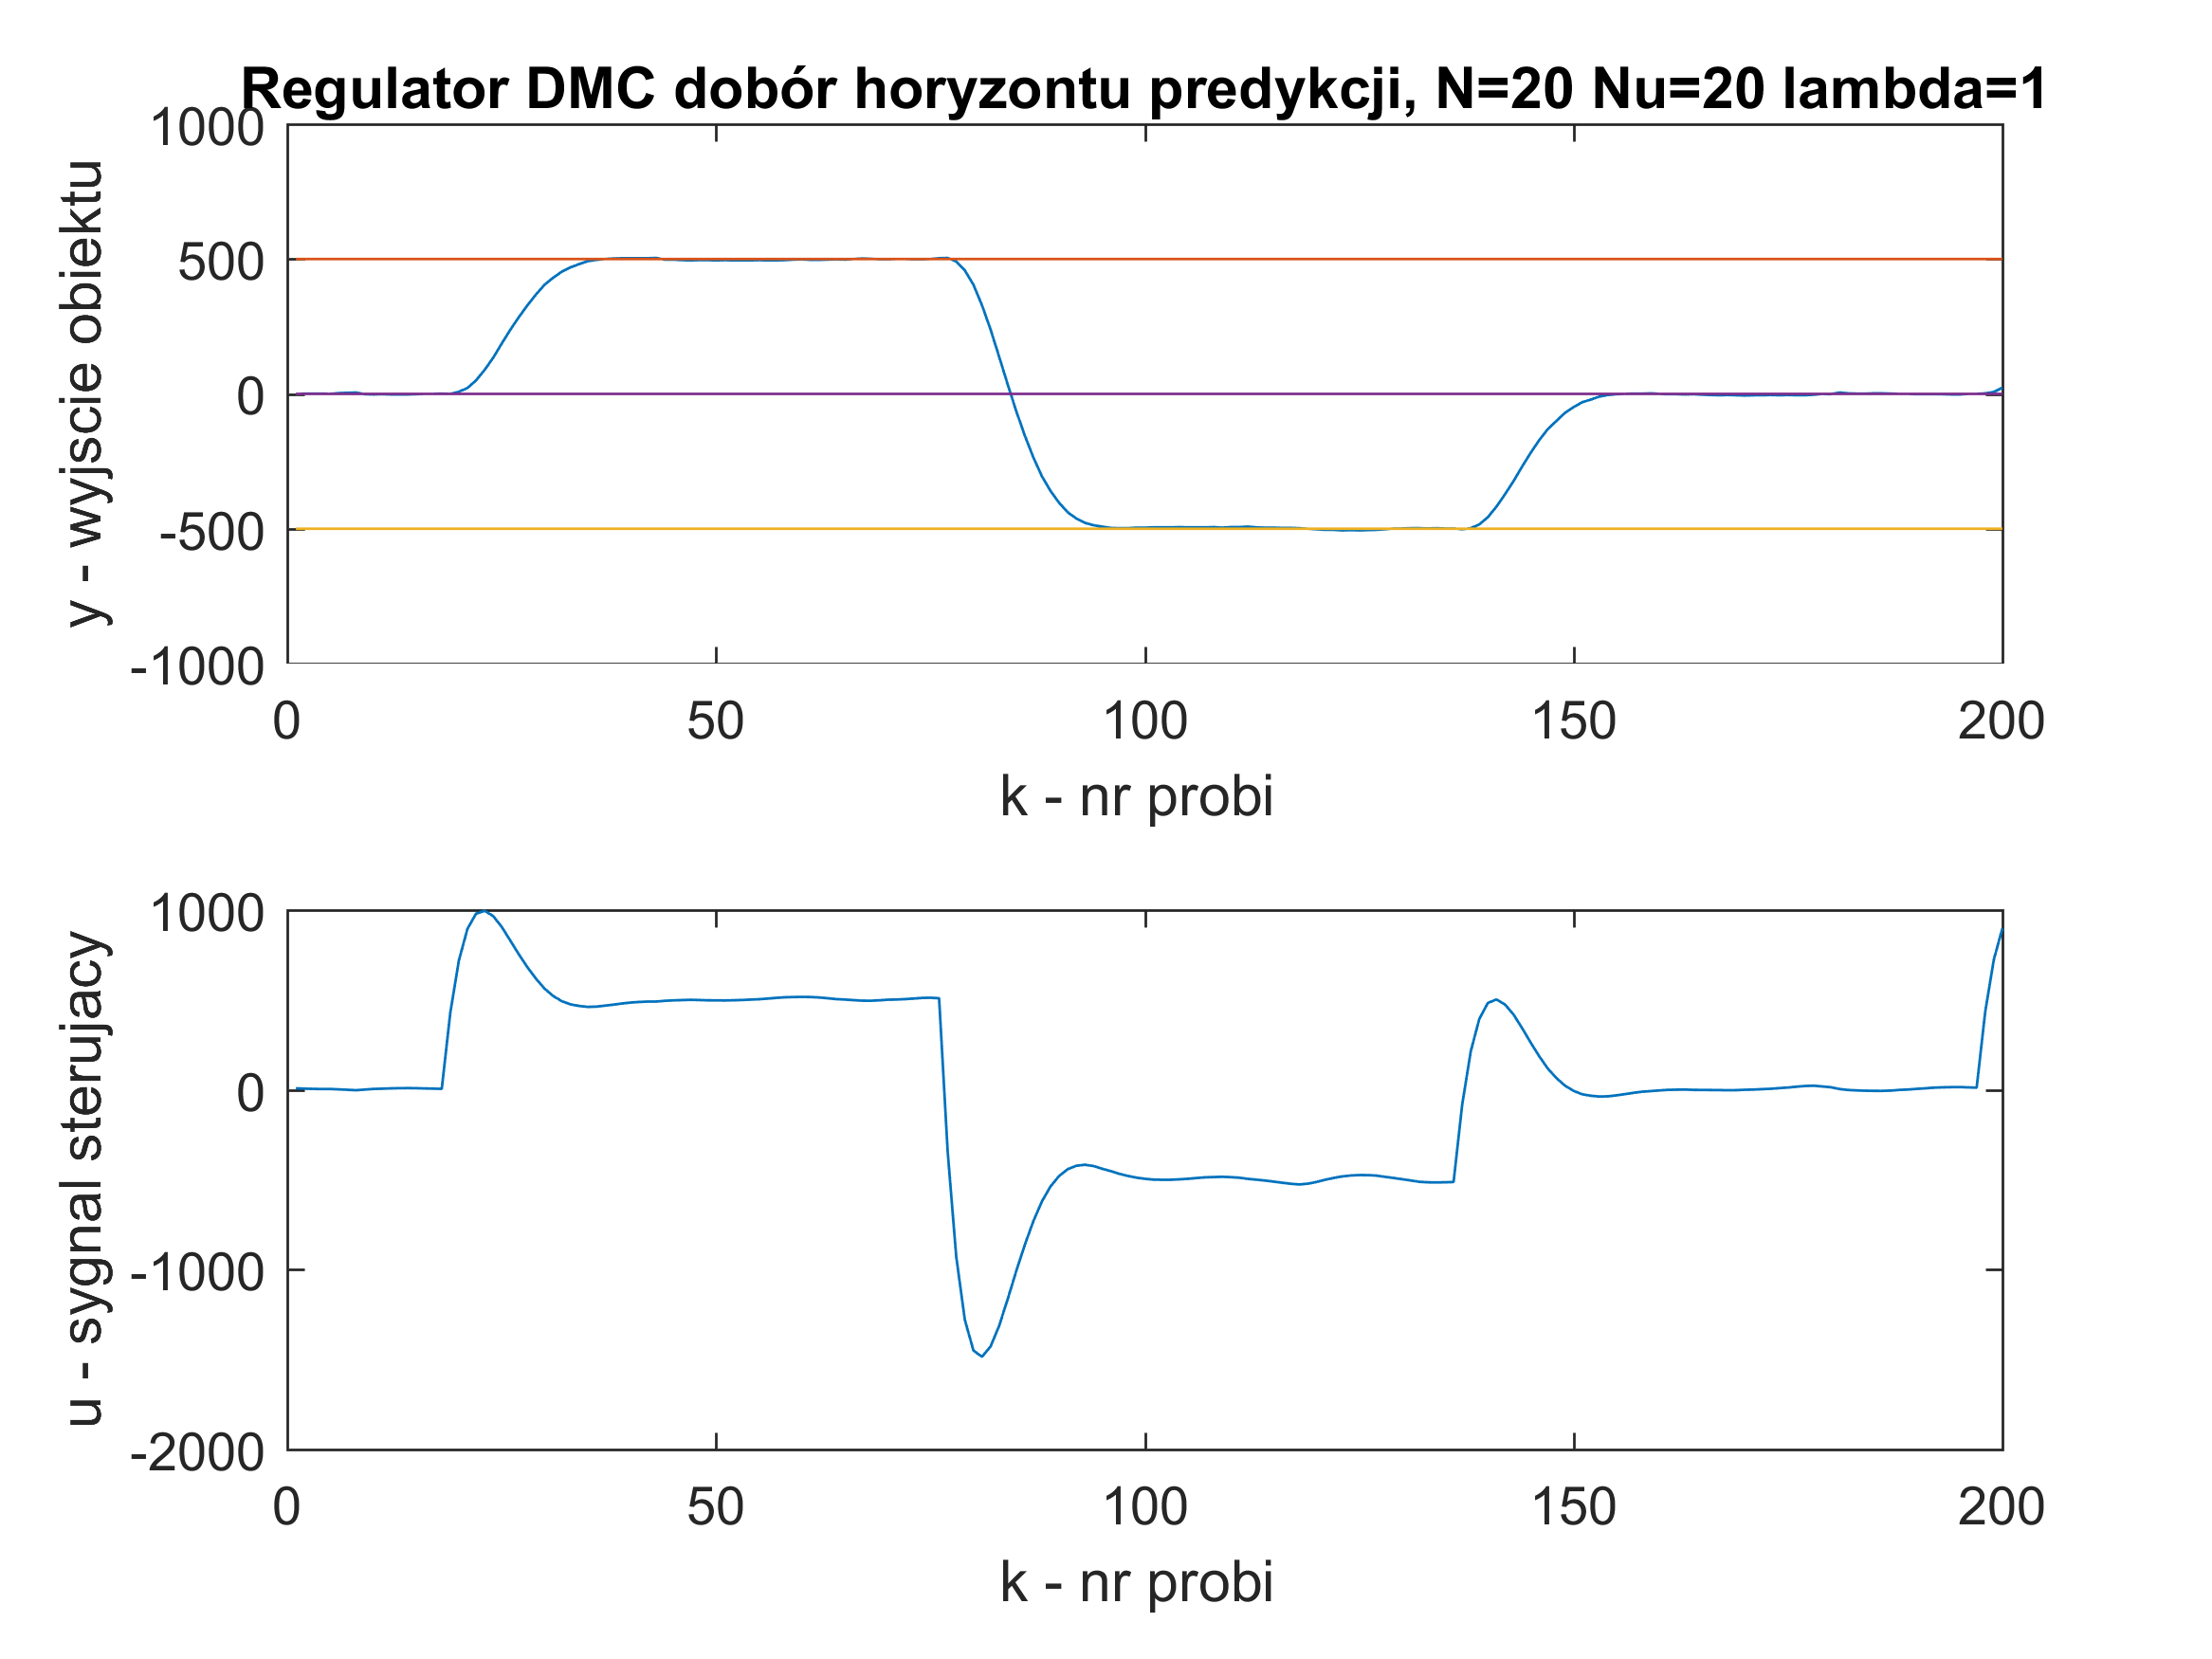
\includegraphics[width=0.9\linewidth]{DMC20201}
	\caption{Przebieg sygnałów przy $N=20$}
	\label{fig:DMC20201}
\end{figure}
\begin{figure}[H]
	\centering
	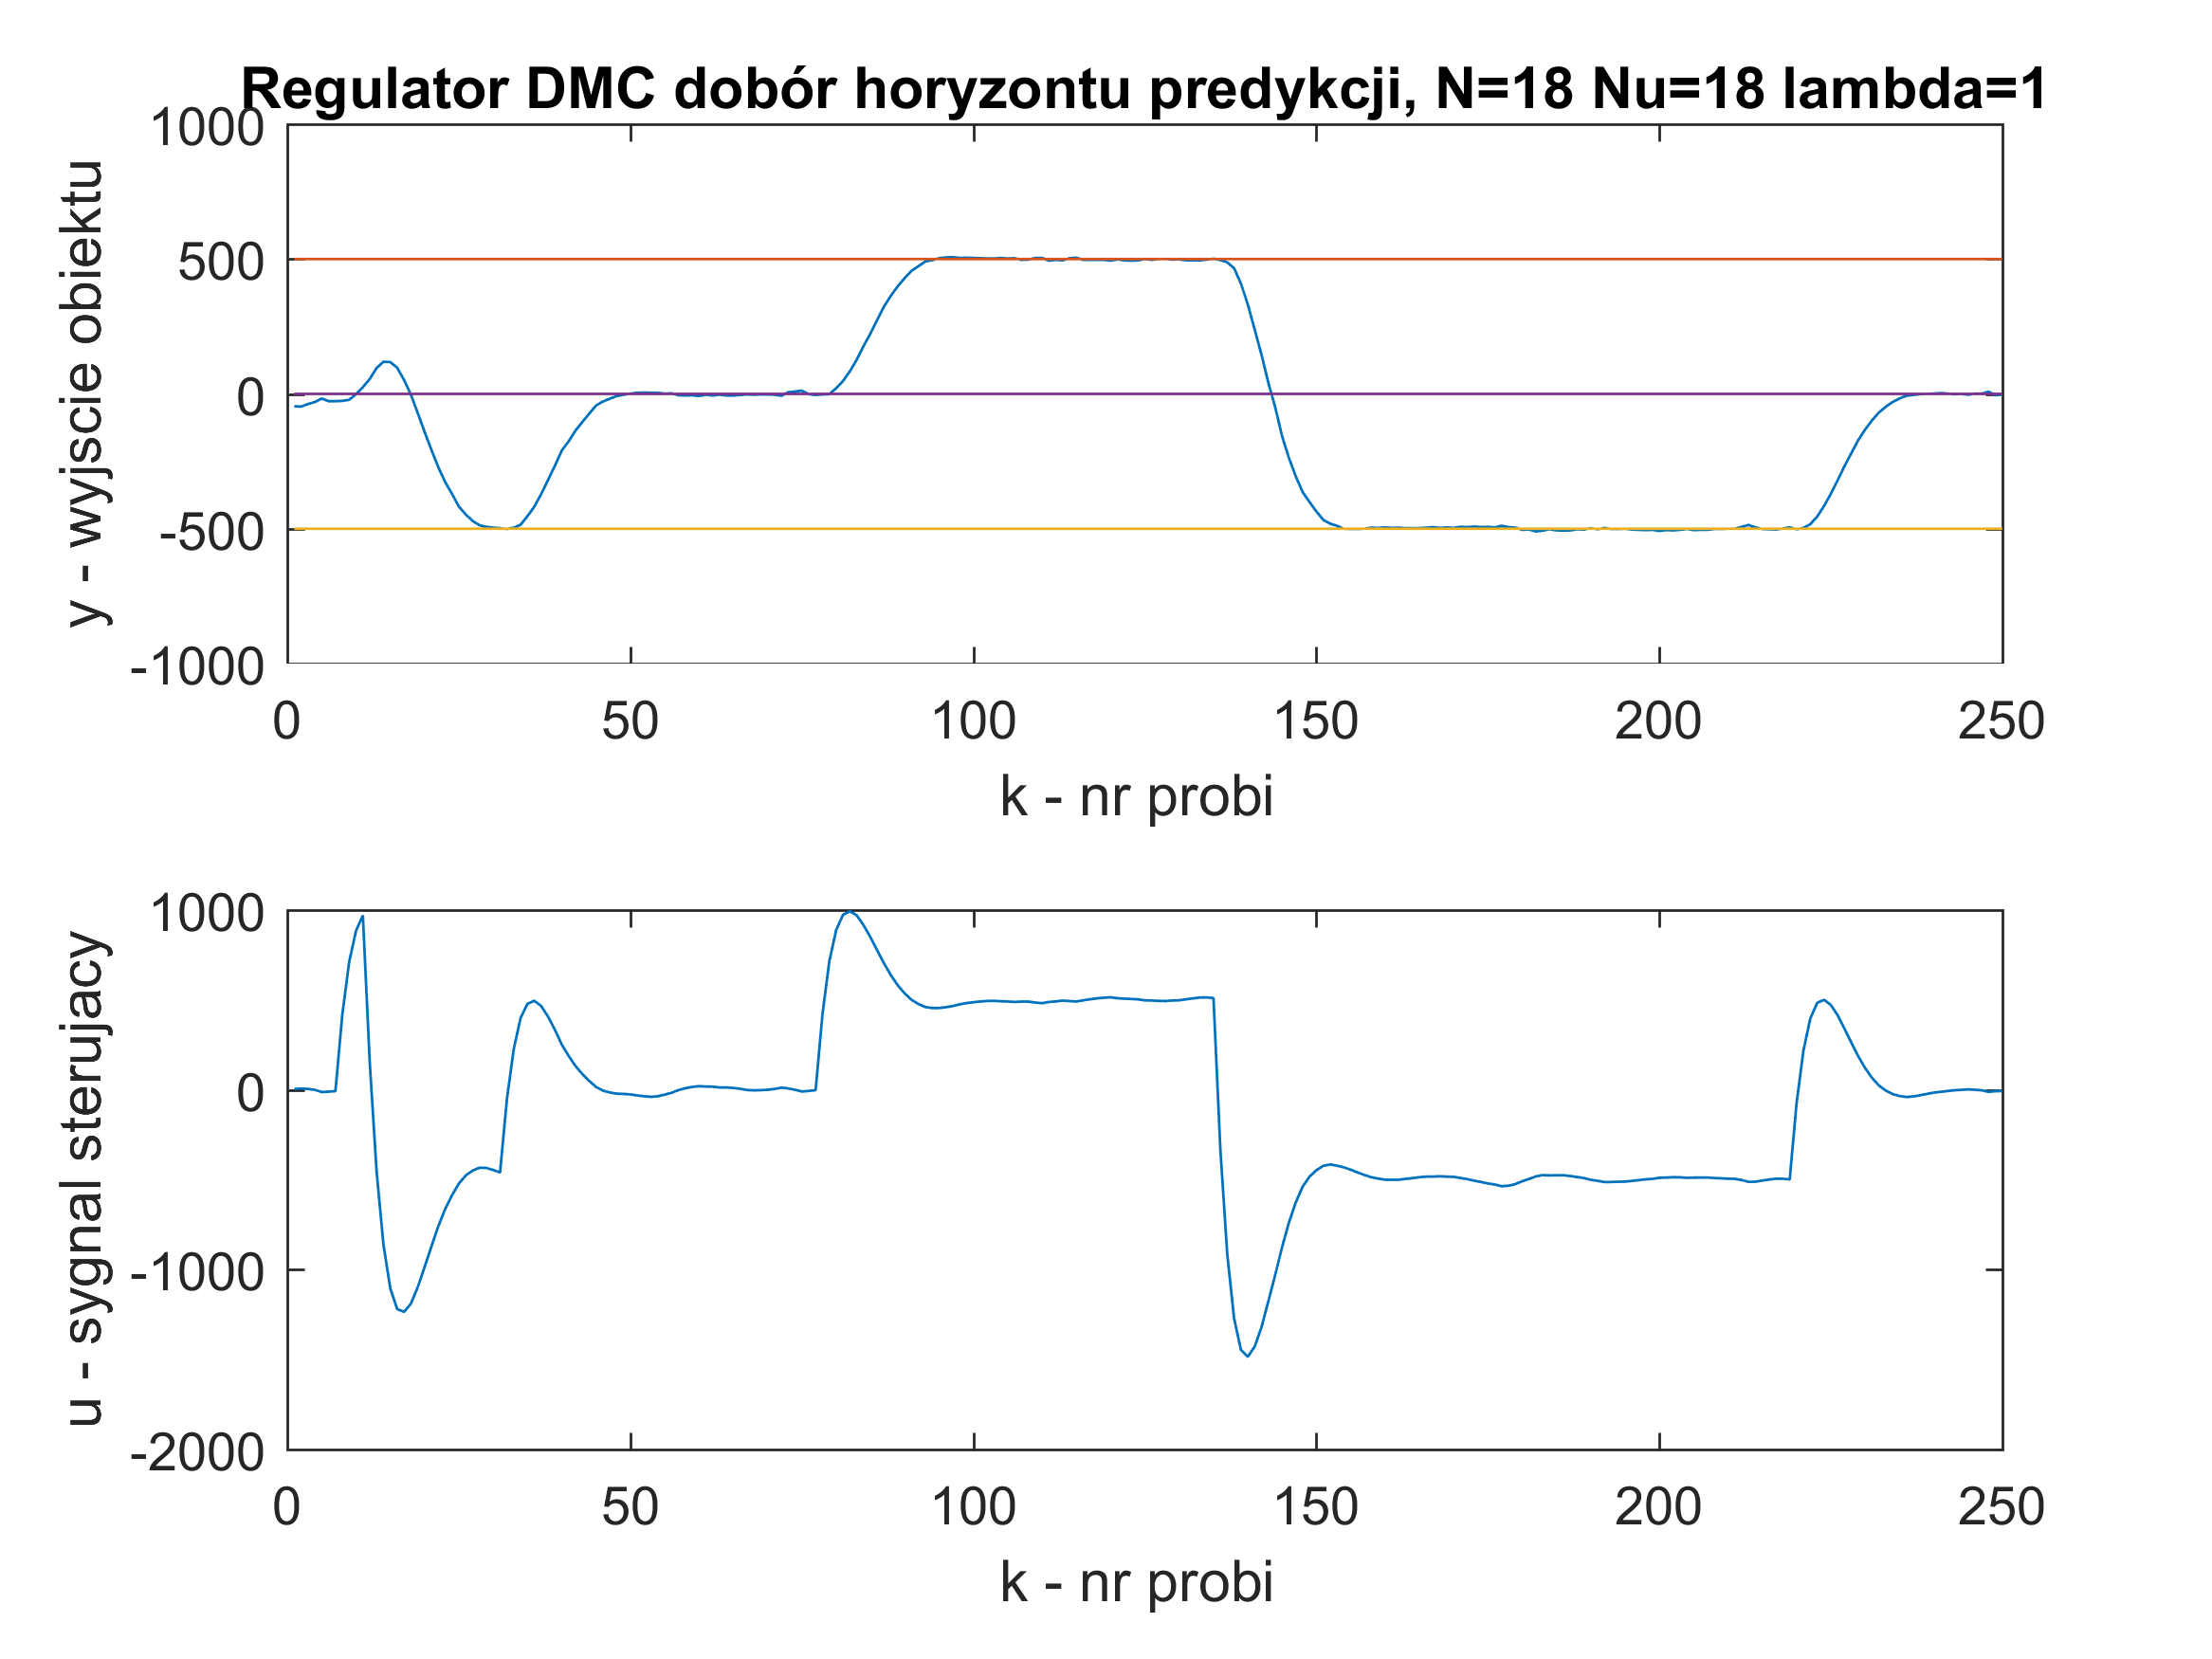
\includegraphics[width=0.9\linewidth]{DMC18181}
	\caption{Przebieg sygnałów przy $N=18$}
	\label{fig:DMC18181}
\end{figure}
\begin{figure}[H]
	\centering
	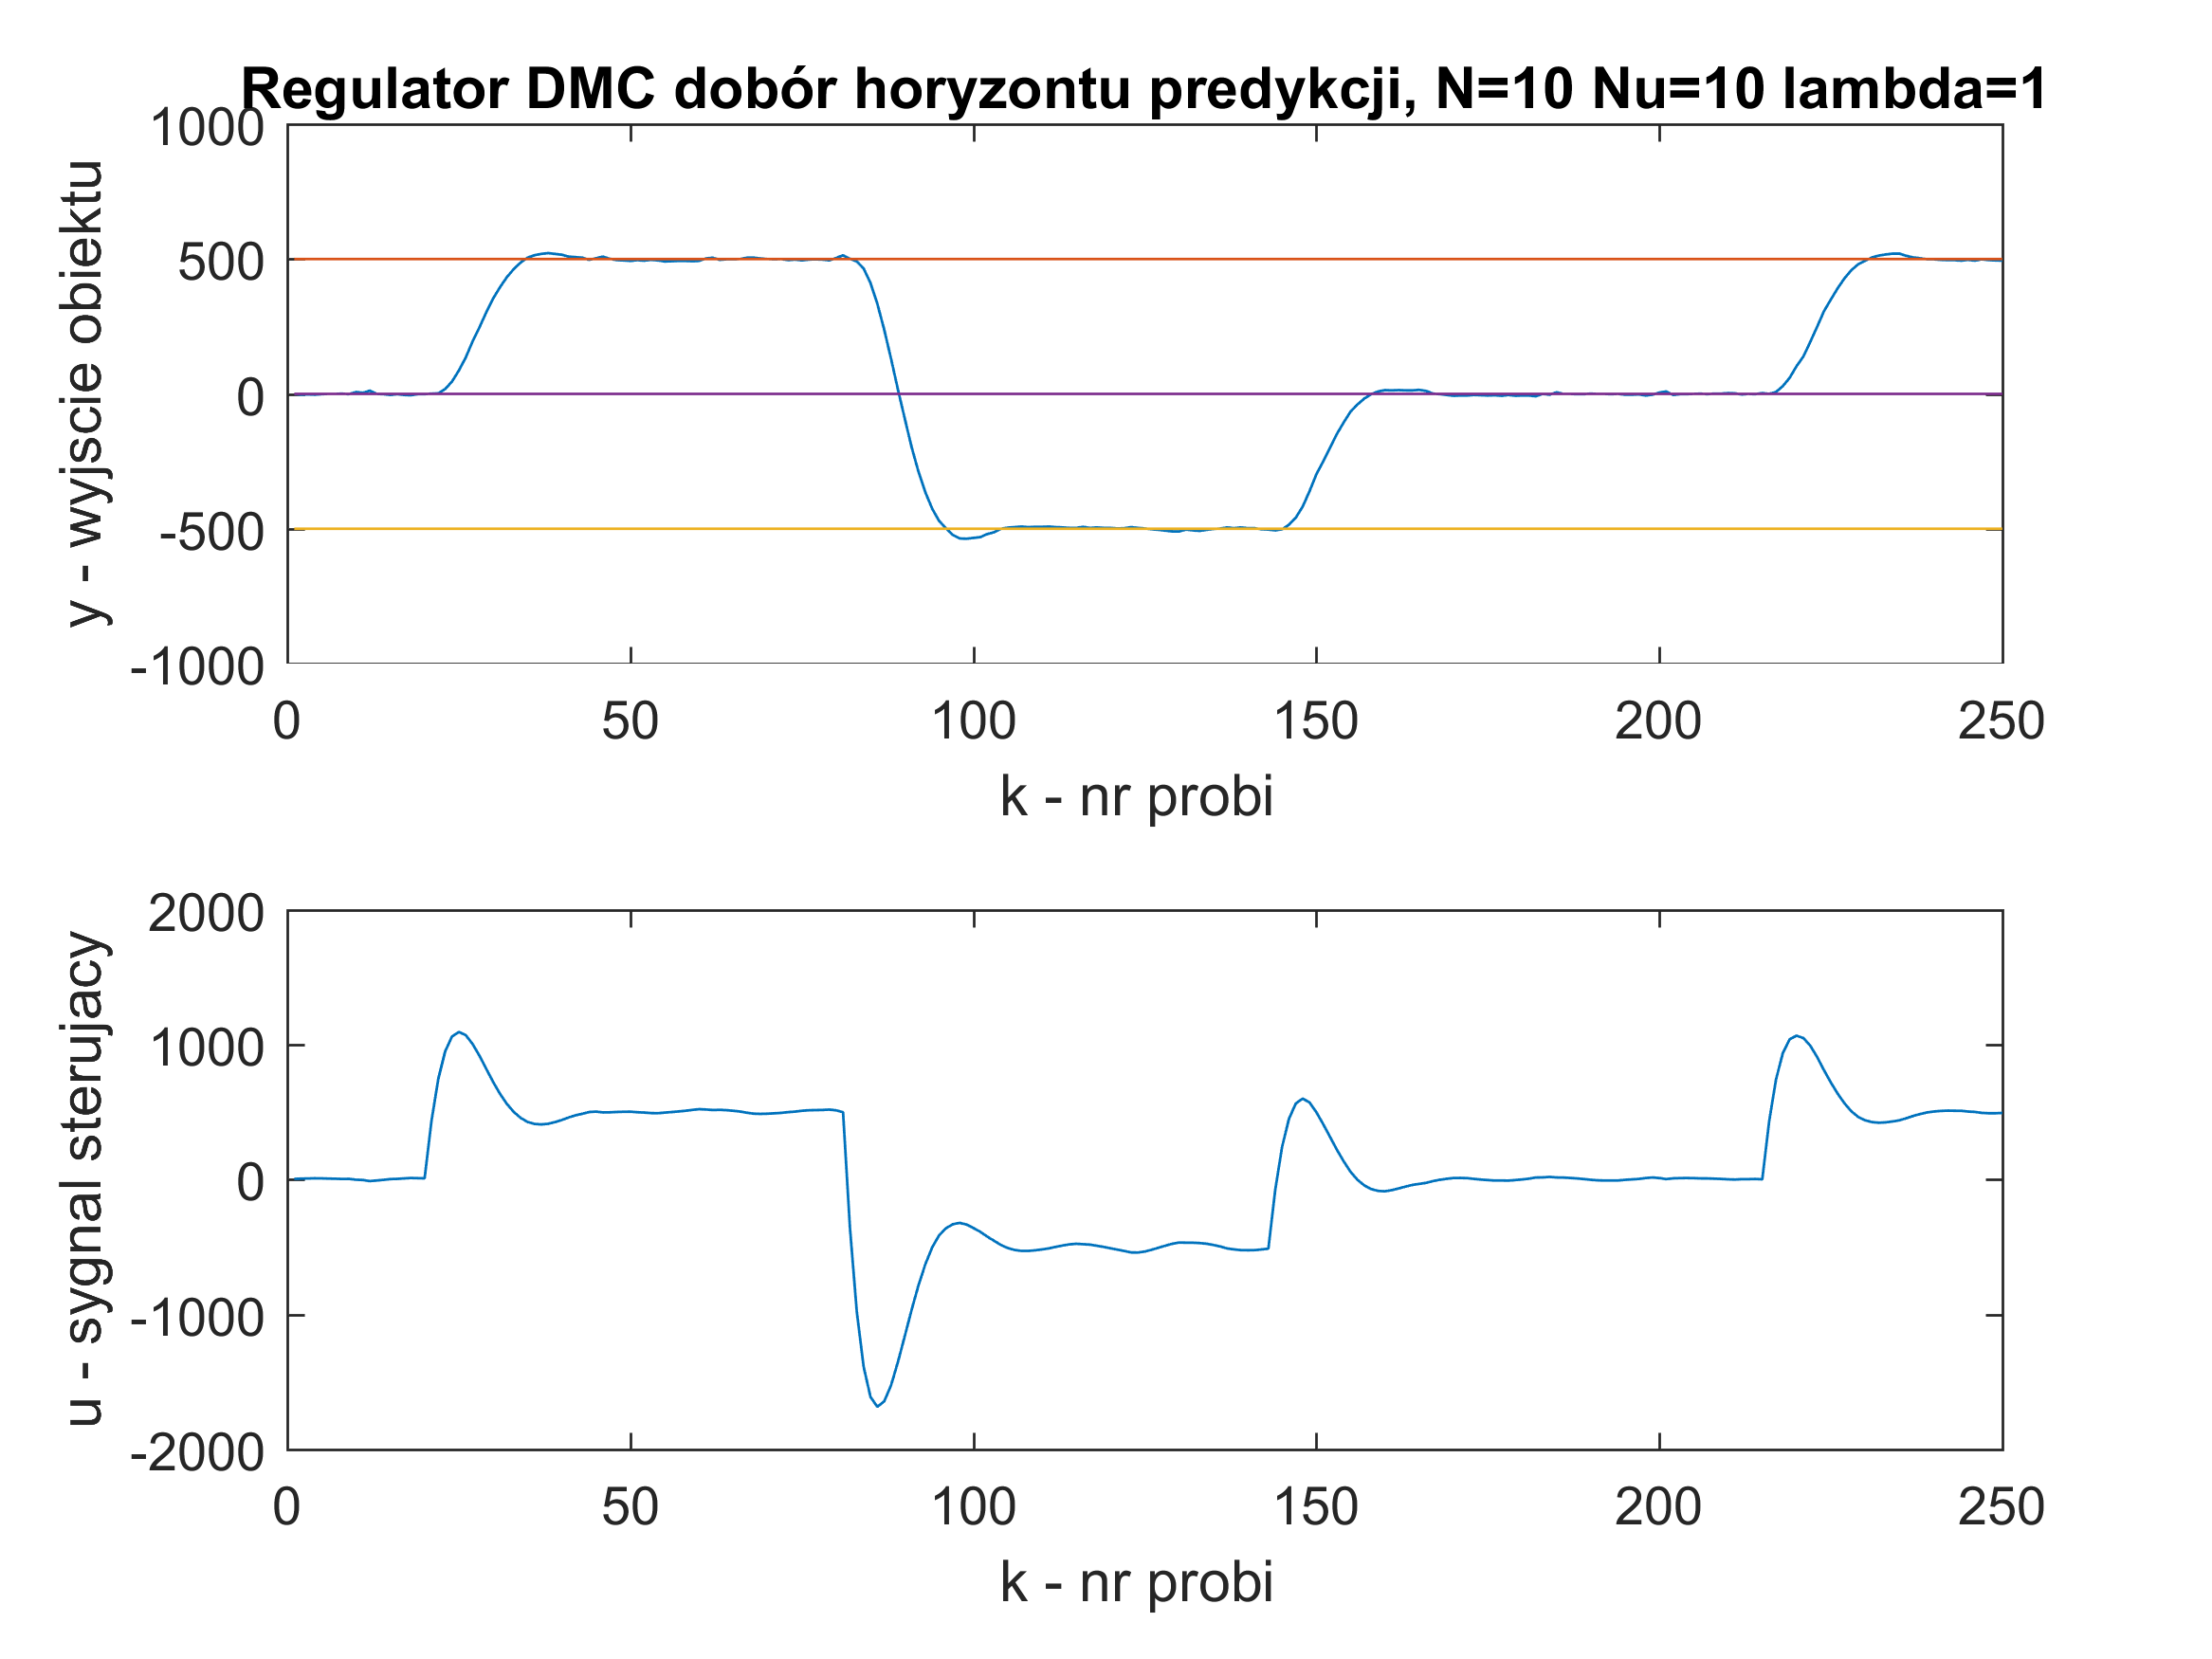
\includegraphics[width=0.9\linewidth]{DMC10101}
	\caption{Przebieg sygnałów przy $N=10$}
	\label{fig:DMC10101}
\end{figure}

Jak widać na wykresach \ref{fig:DMC60601}, \ref{fig:DMC30301}, \ref{fig:DMC20201}, \ref{fig:DMC18181} pomimo zmniejszania parametru $N$, jakość regulacji pozostaje niezmienna, czyli regulatory osiągają podobne czasy regulacji oraz wartość przesterowania jest znikoma. Dopiero zmniejszenie parametru $N$ do wartości 10 spowodowało pogorszenie się trajektorii sygnału wyjściowego - widać zauważalne przeregulowanie. Z tego powodu przyjęłyśmy $N=18$.

\subsection{Wyznaczenie horyzontu sterowania}
Sposób wyznaczenia horyzontu sterowania $N_{u}$ jest podobny do wyznaczania parametru $N$. Na początku przyjmuje się $N_{u}=N$, a następnie stopniowo się go zmniejsza do momentu zauważenia widocznego pogorszenia jakości trajektorii sygnału wyjściowego. W eksperymentach przyjmuje się $\lambda=1$.
\begin{figure}[H]
	\centering
	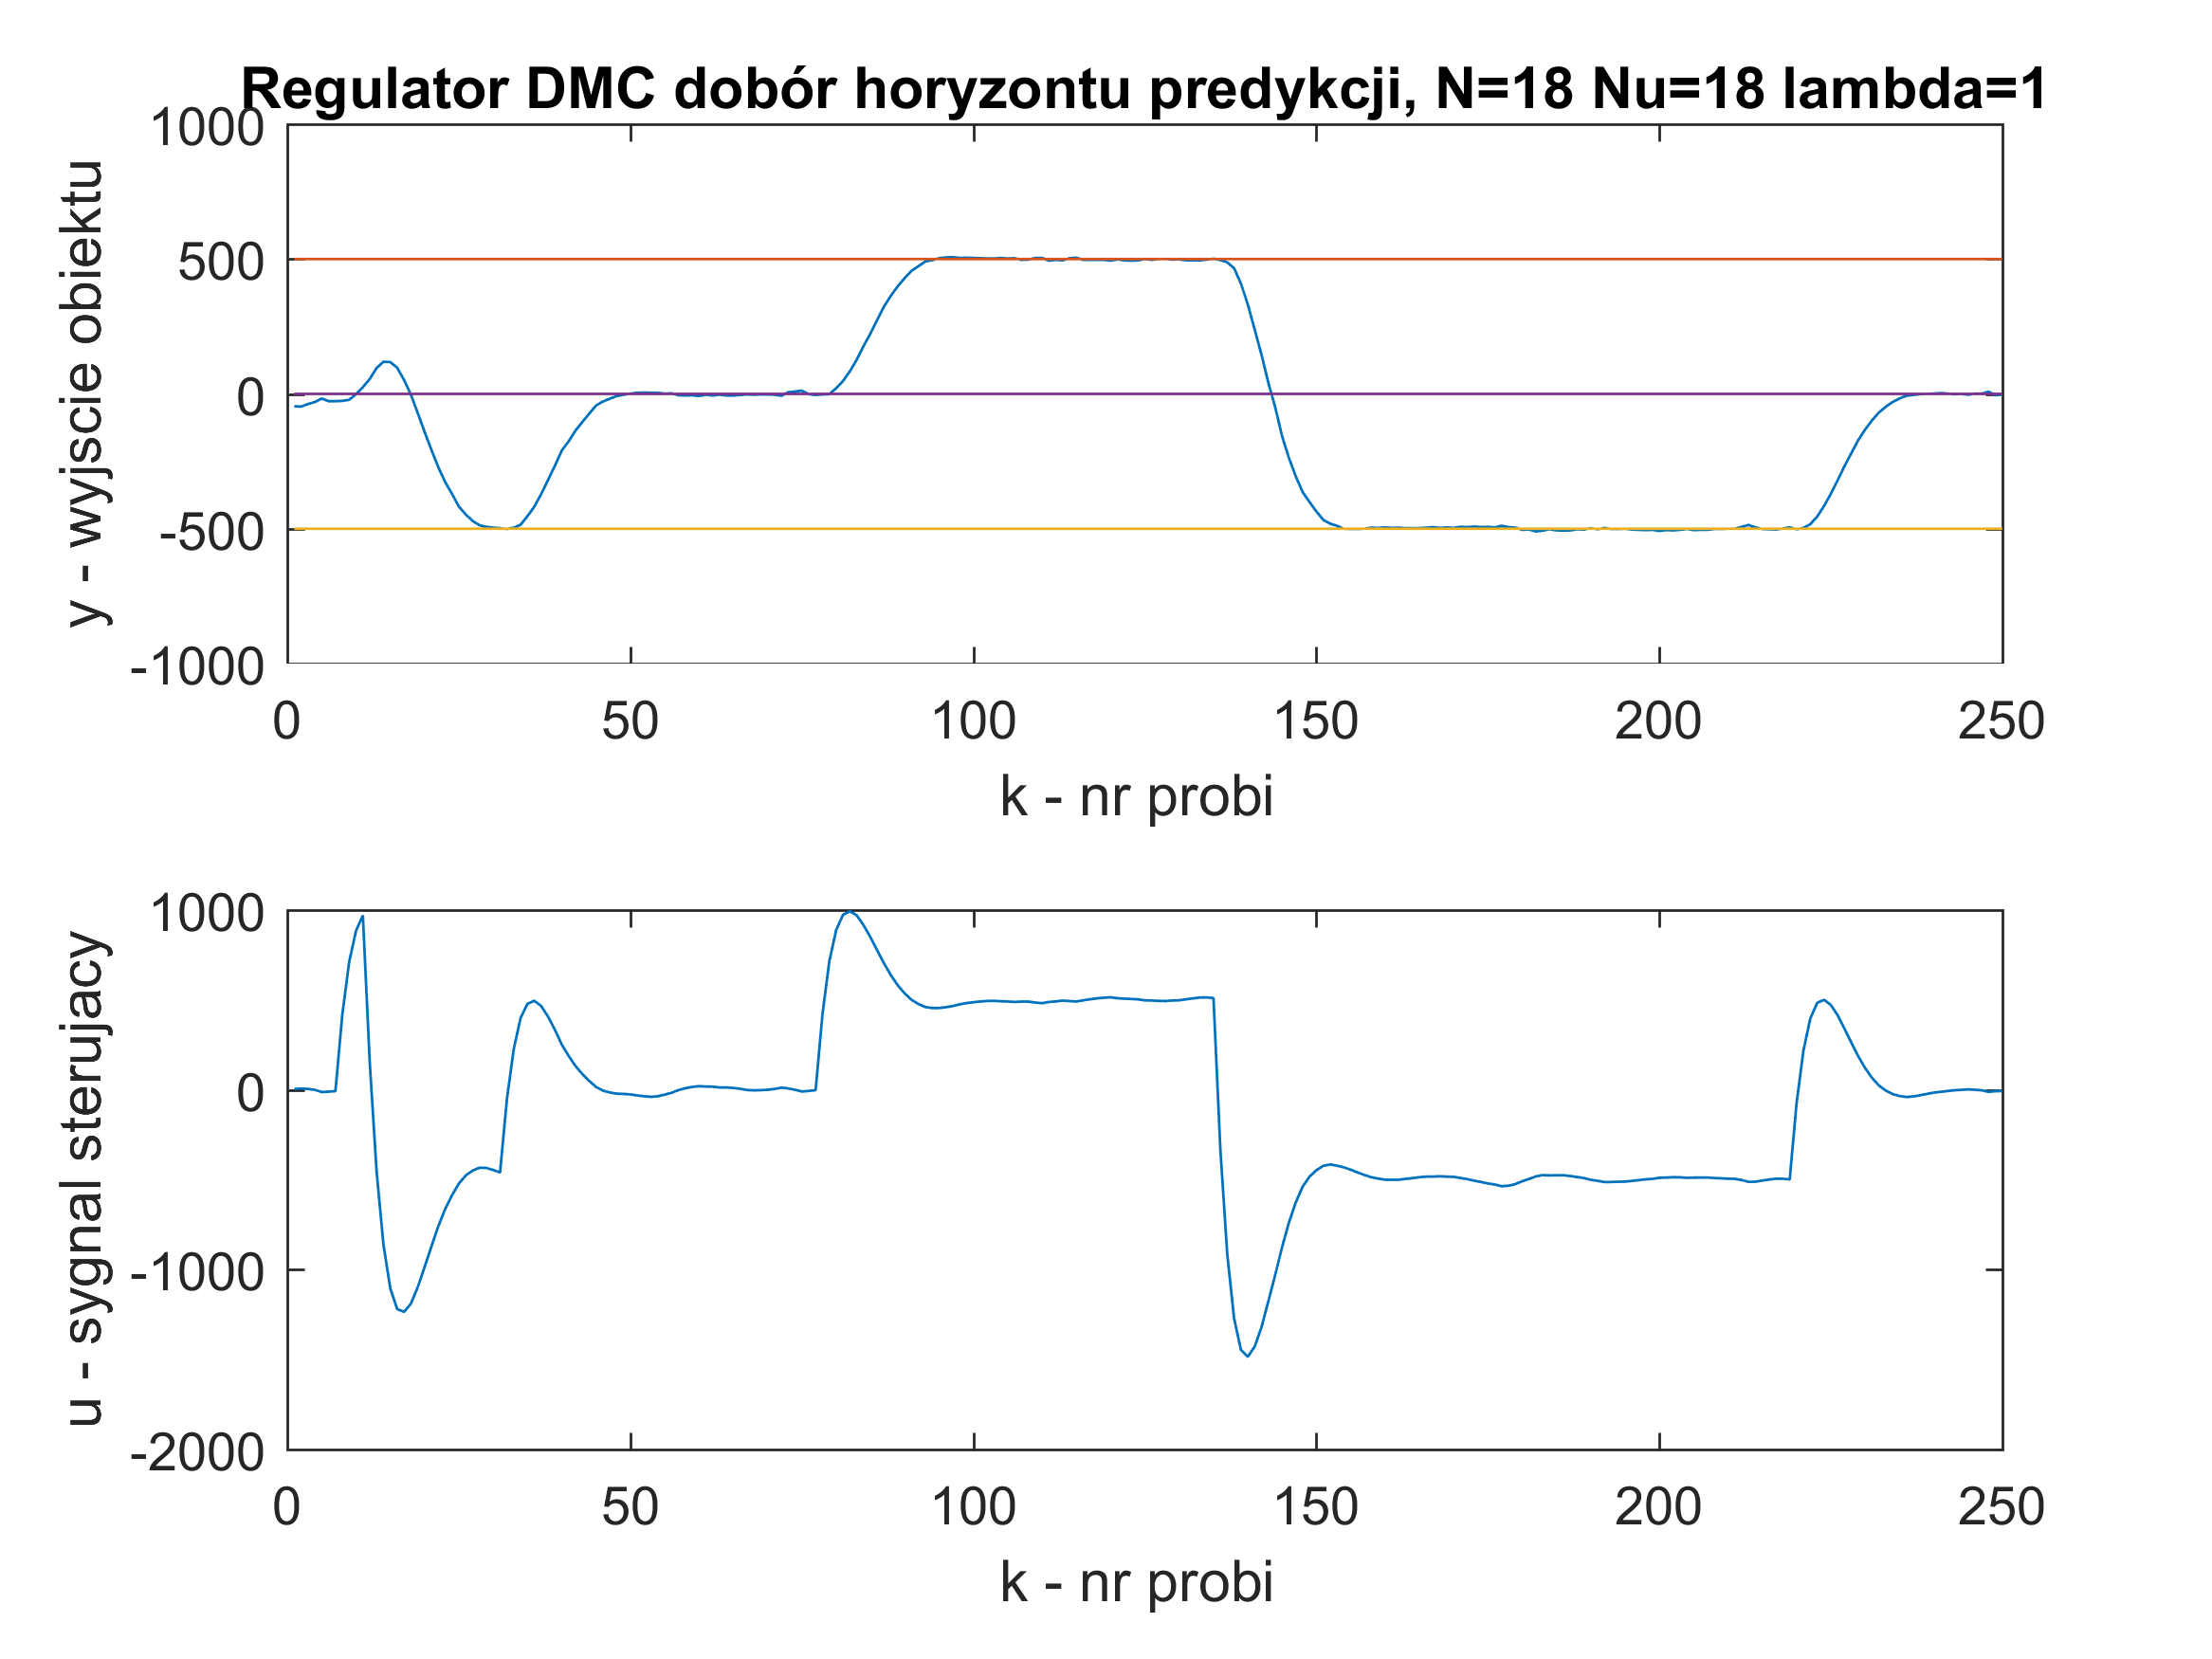
\includegraphics[width=0.9\linewidth]{DMC18181}
	\caption{Przebieg sygnałów przy $N_{u}=18$}
	\label{fig:DMC18181}
\end{figure}
\begin{figure}[H]
	\centering
	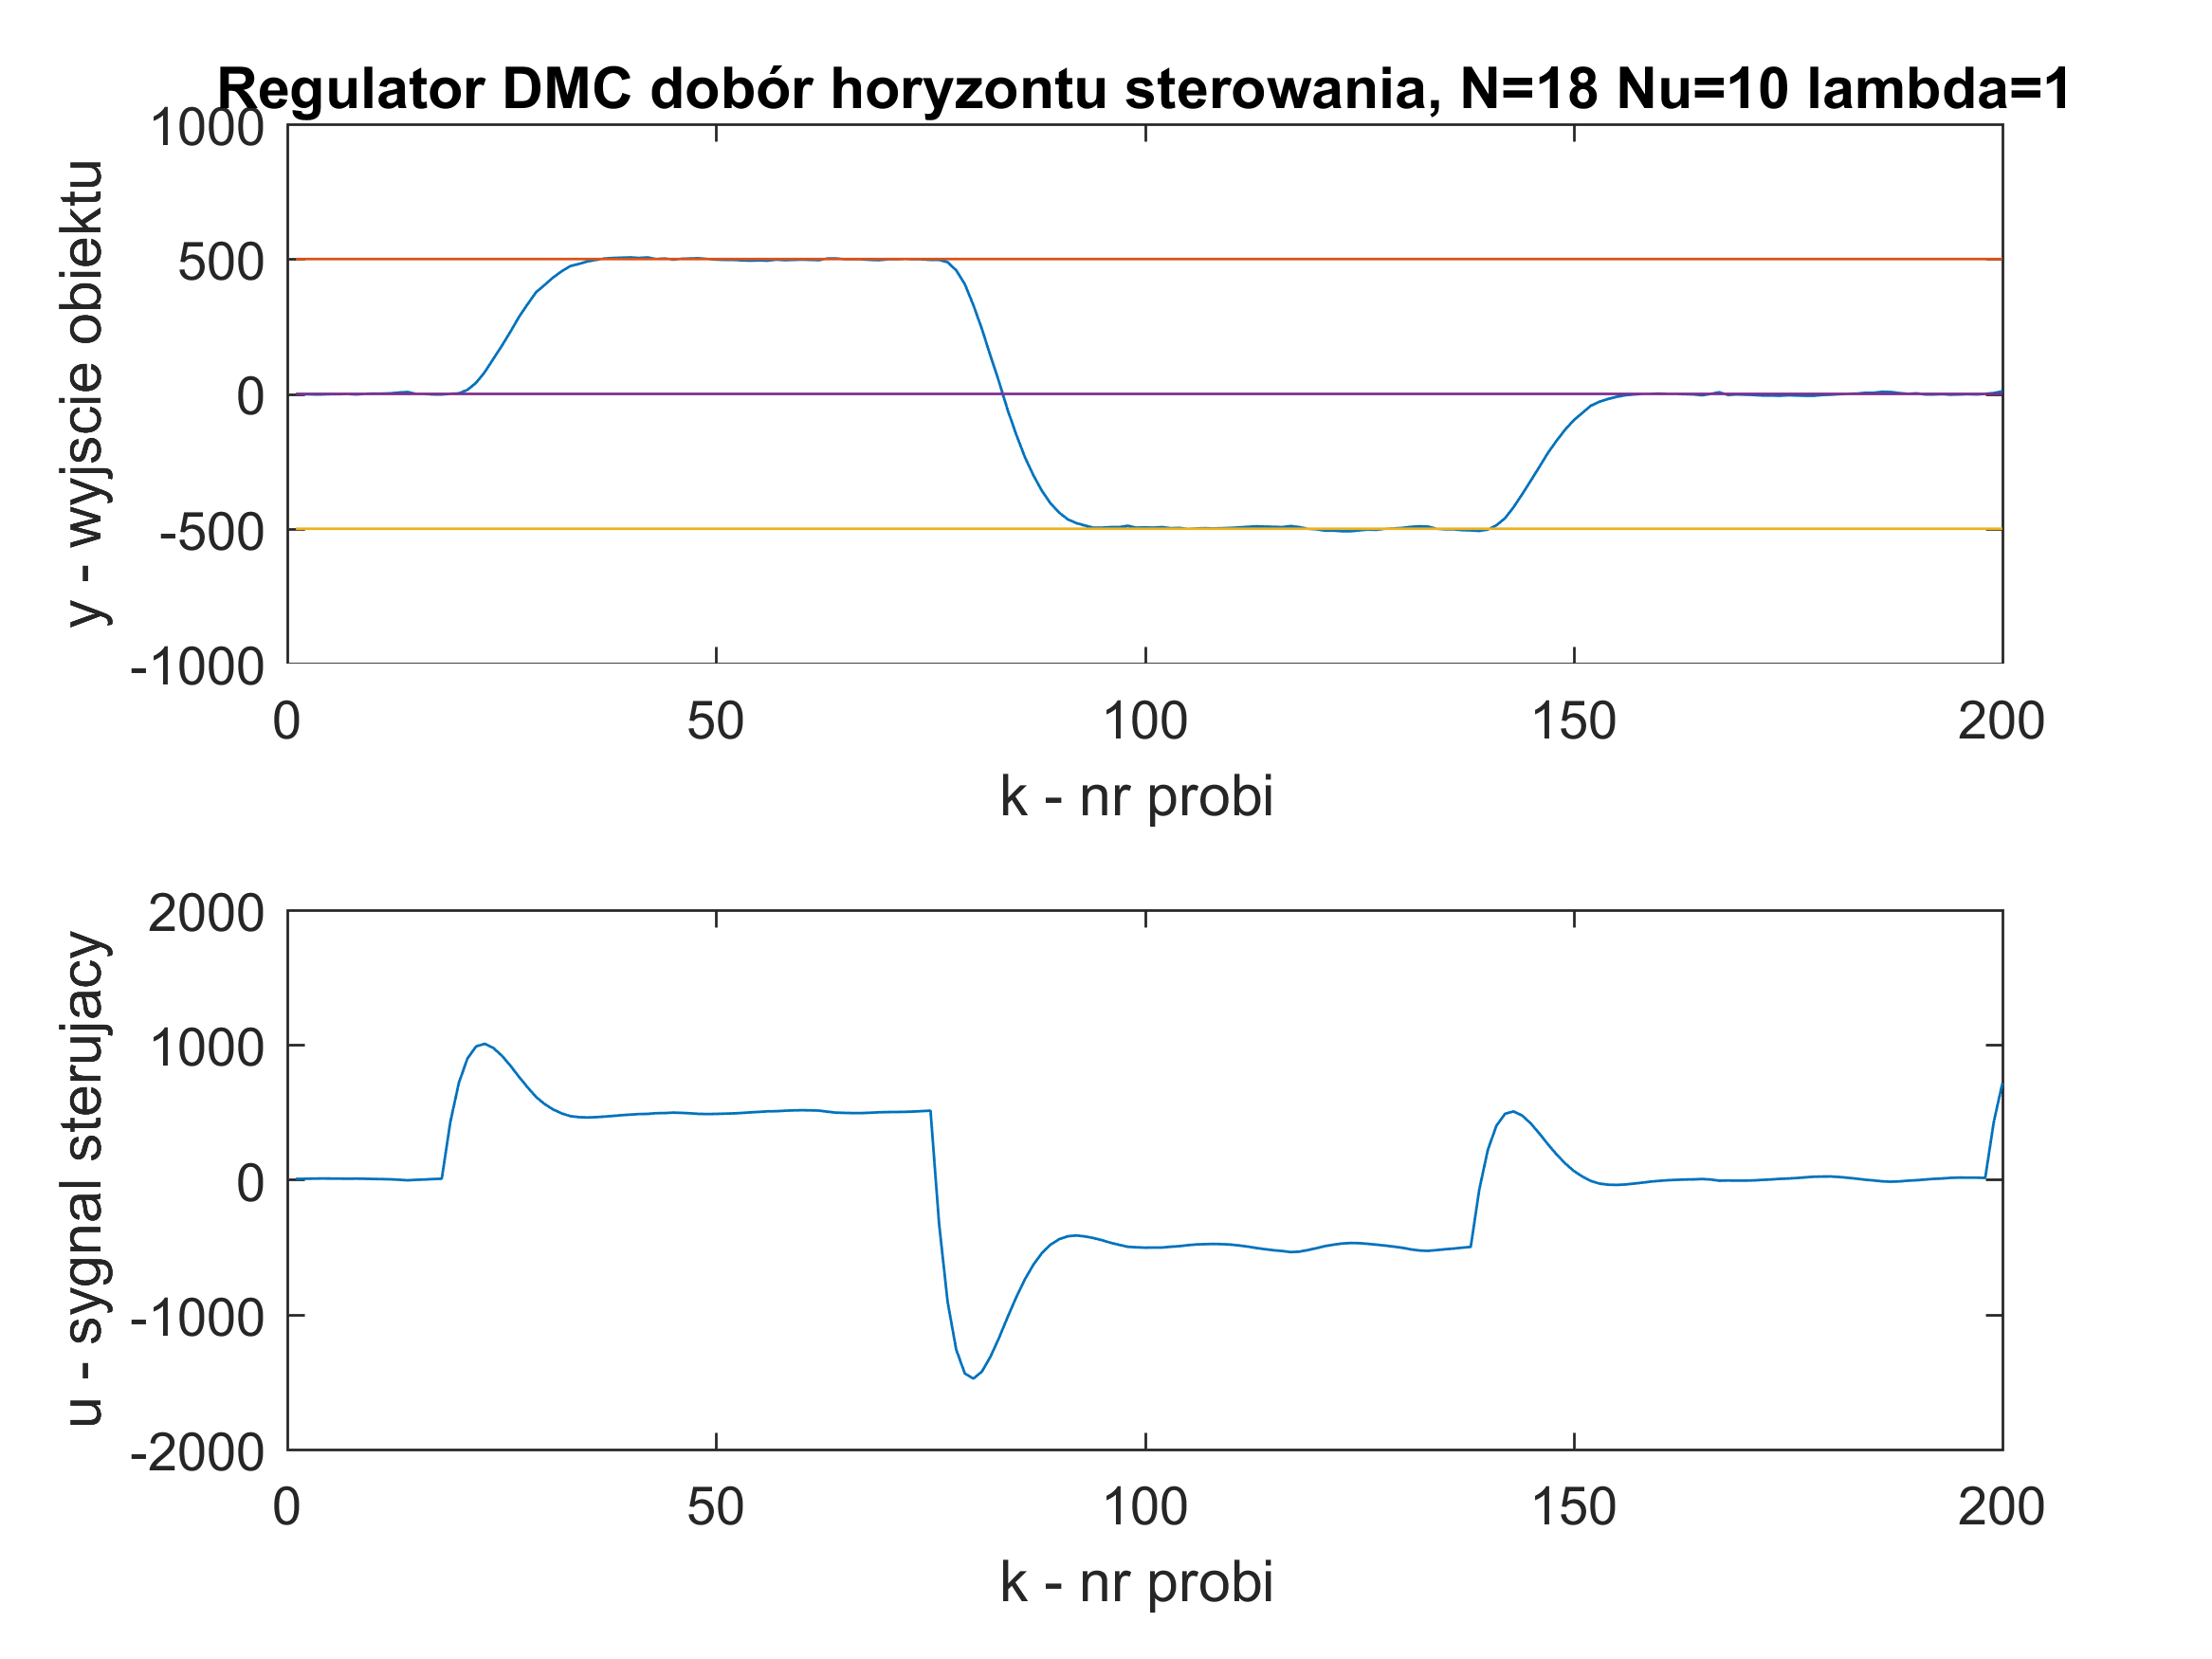
\includegraphics[width=0.9\linewidth]{DMC18101}
	\caption{Przebieg sygnałów przy $N_{u}=10$}
	\label{fig:DMC18101}
\end{figure}
\begin{figure}[H]
	\centering
	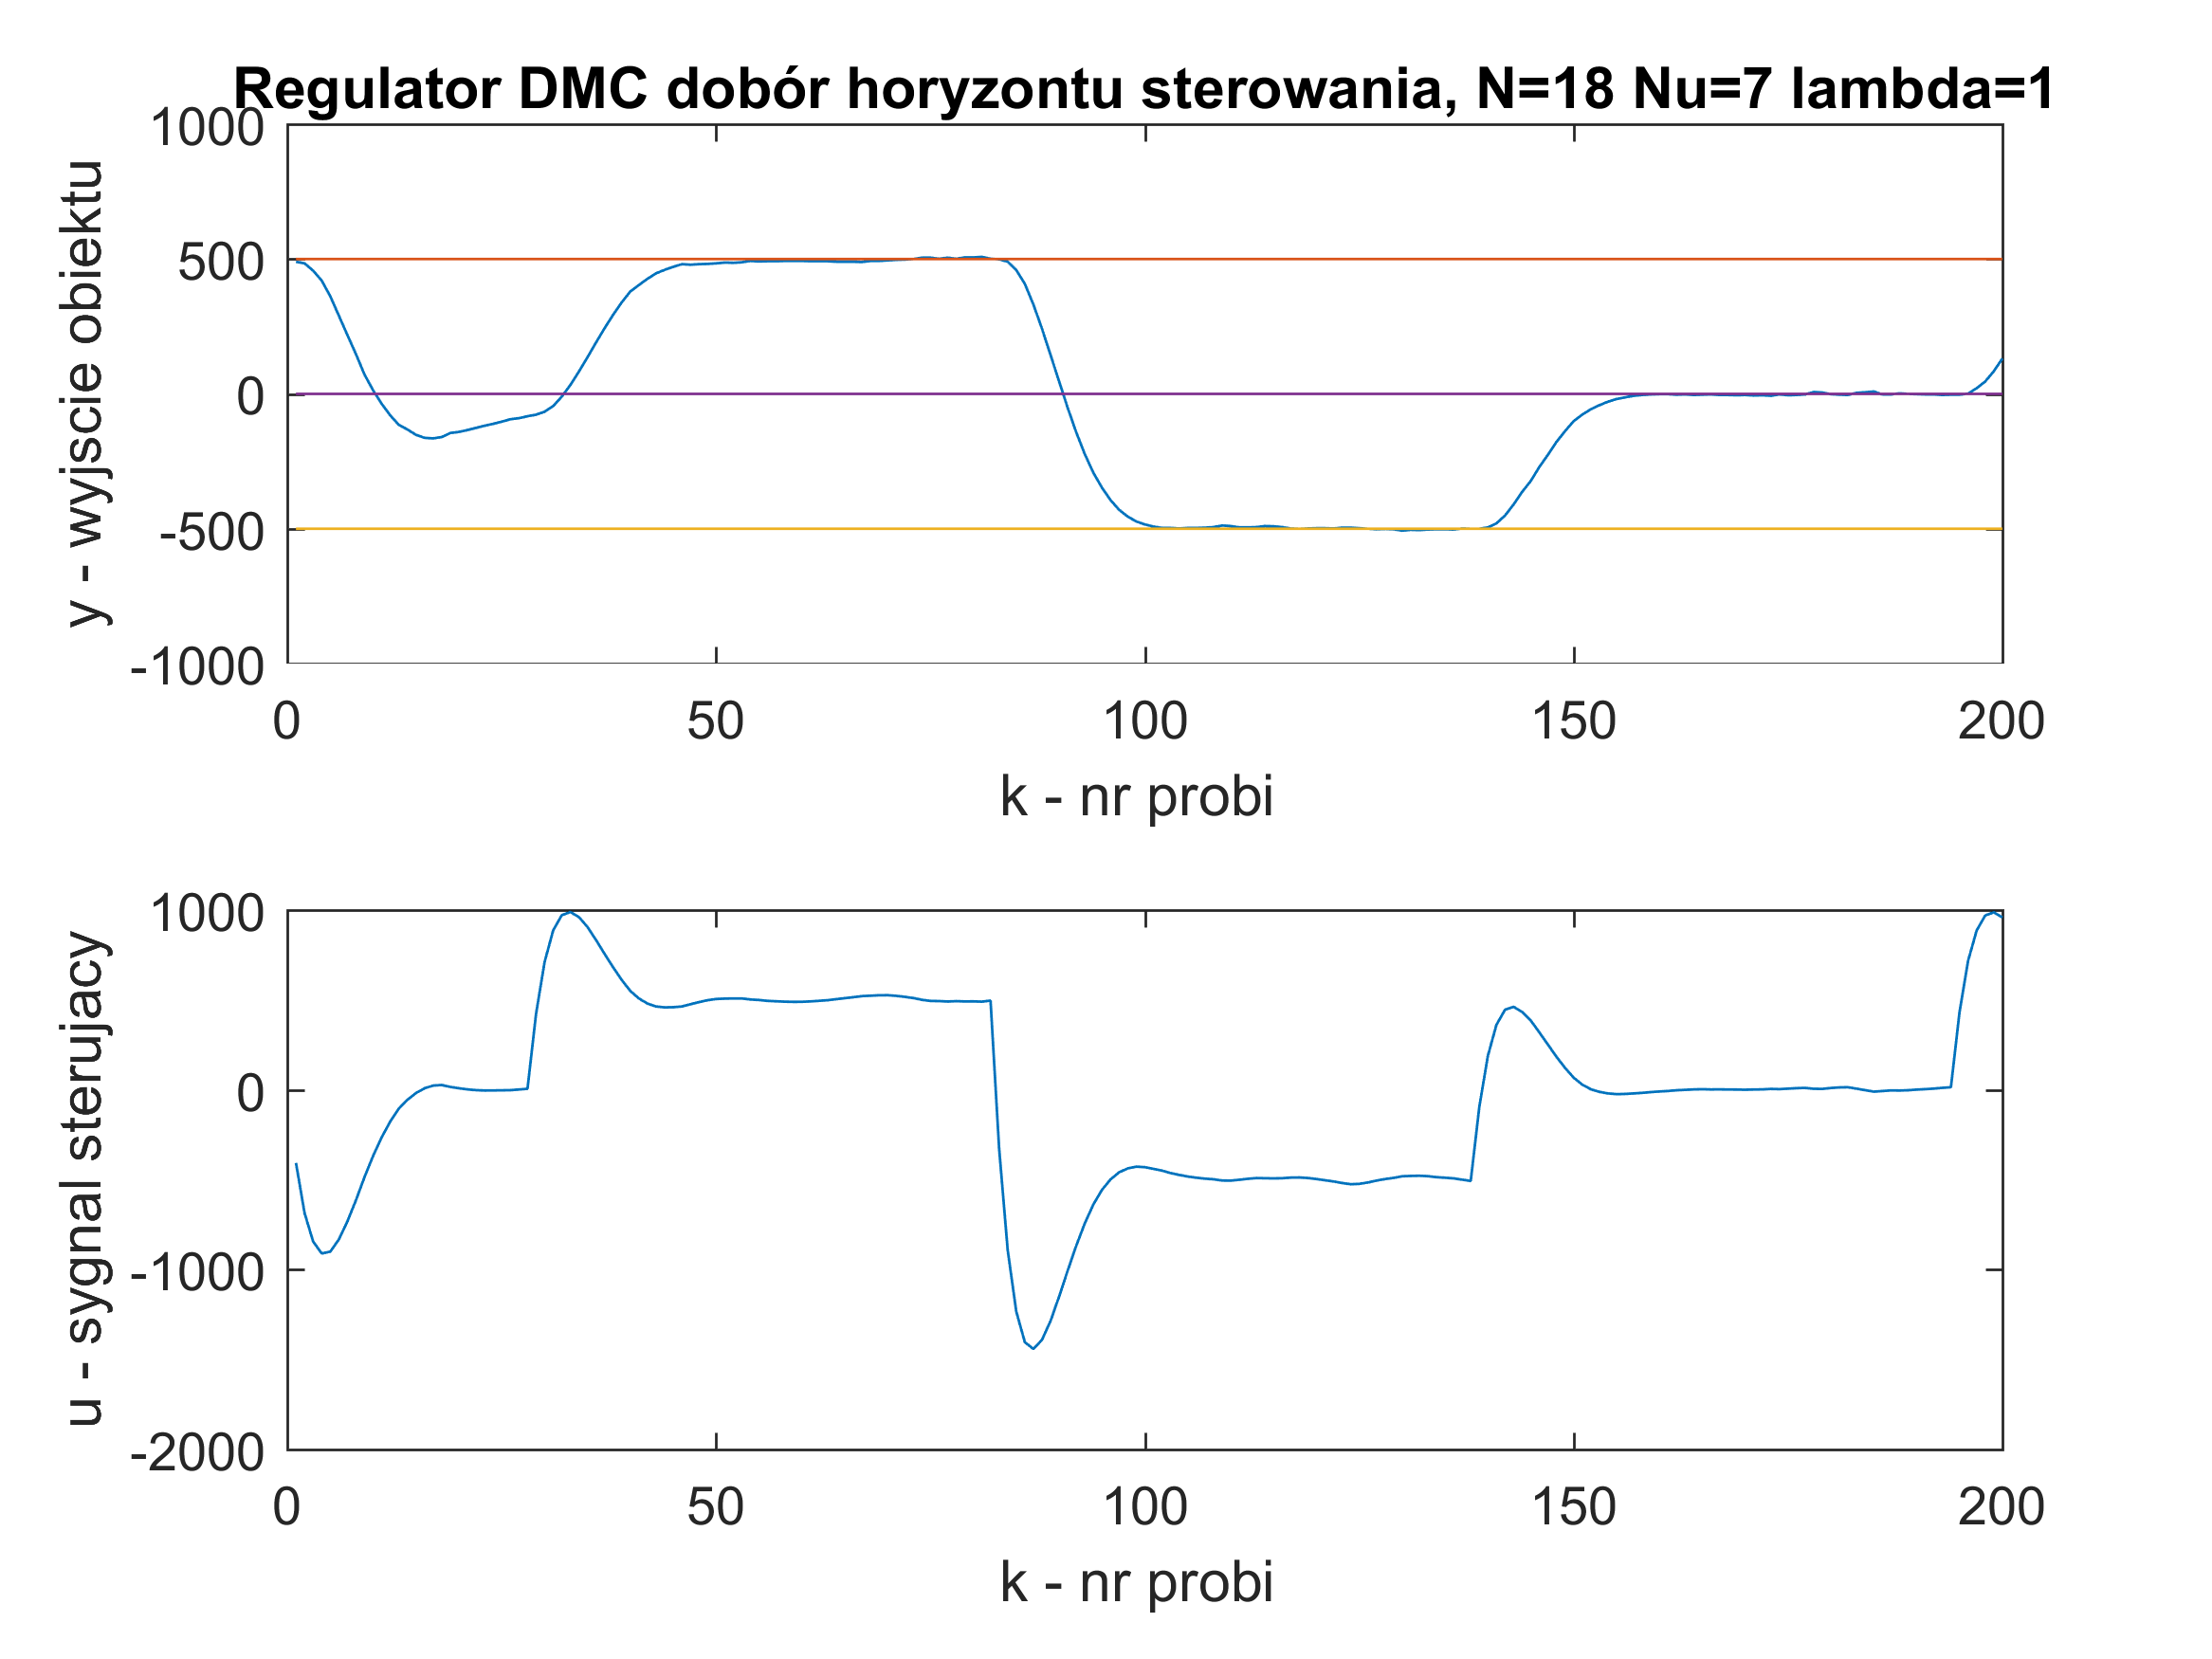
\includegraphics[width=0.9\linewidth]{DMC1871}
	\caption{Przebieg sygnałów przy $N_{u}=7$}
	\label{fig:DMC1871}
\end{figure}
\begin{figure}[H]
	\centering
	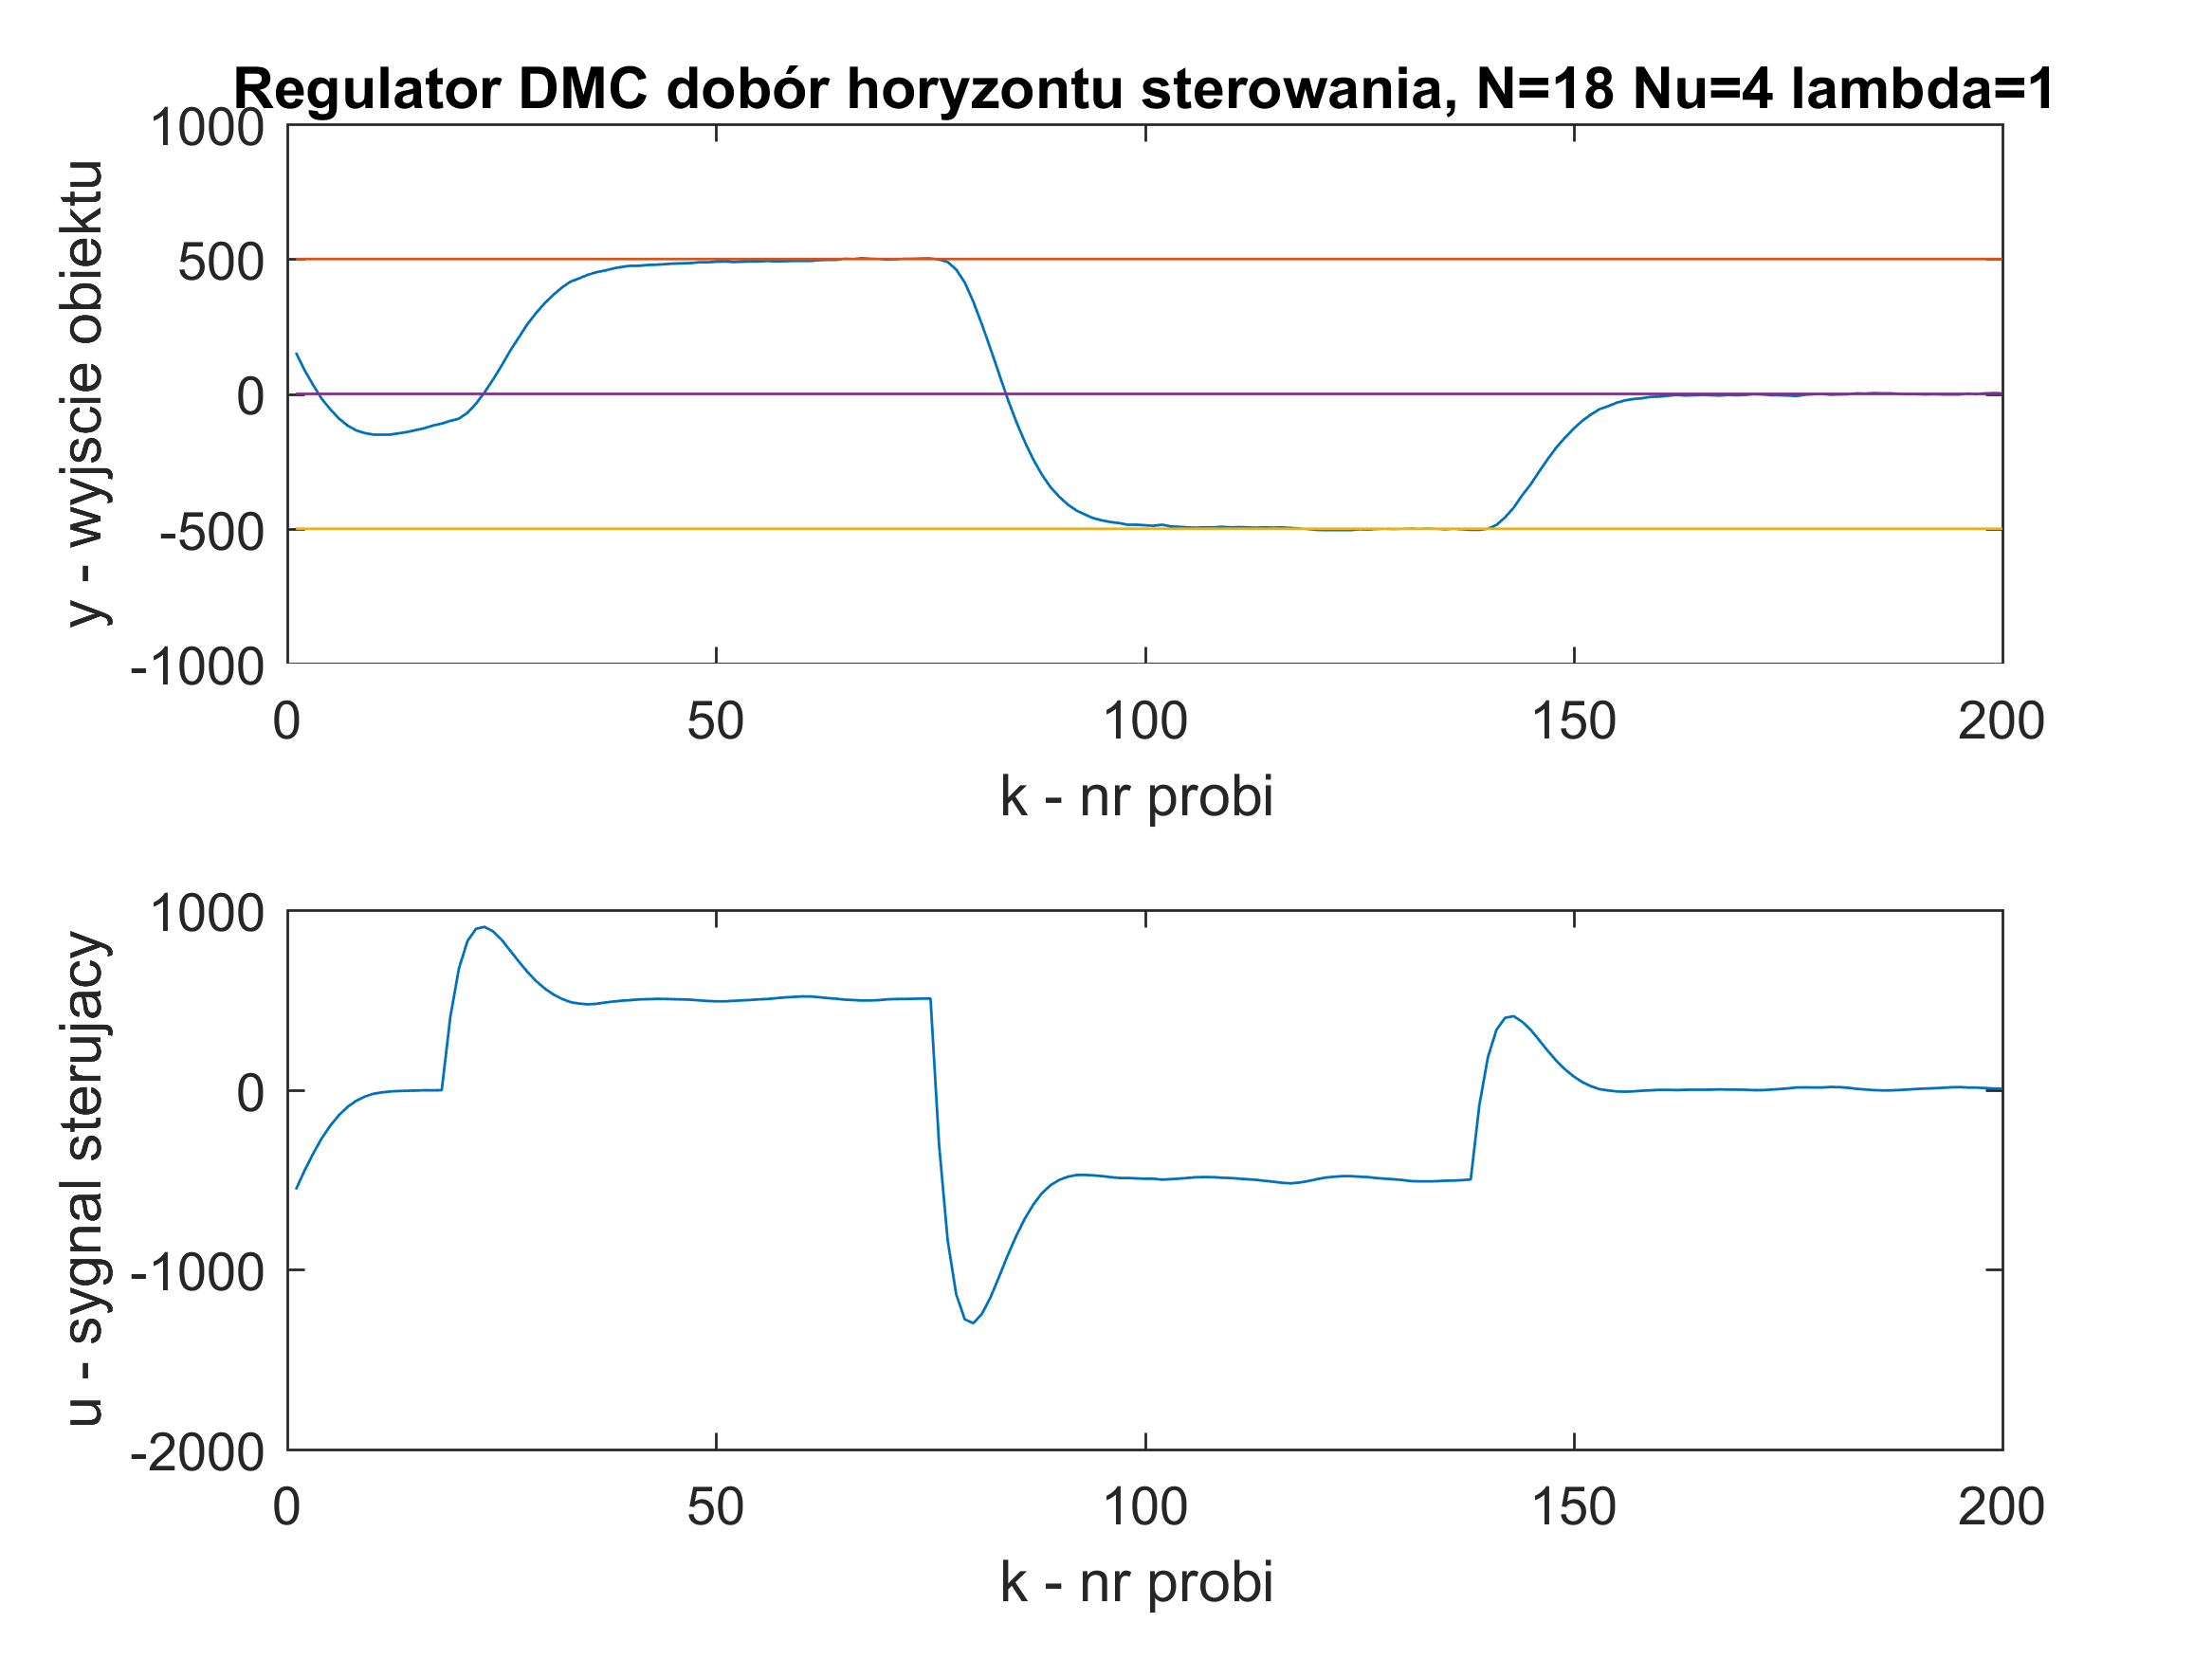
\includegraphics[width=0.9\linewidth]{DMC1841}
	\caption{Przebieg sygnałów przy $N_{u}=4$}
	\label{fig:DMC1841}
\end{figure}
\begin{figure}[H]
	\centering
	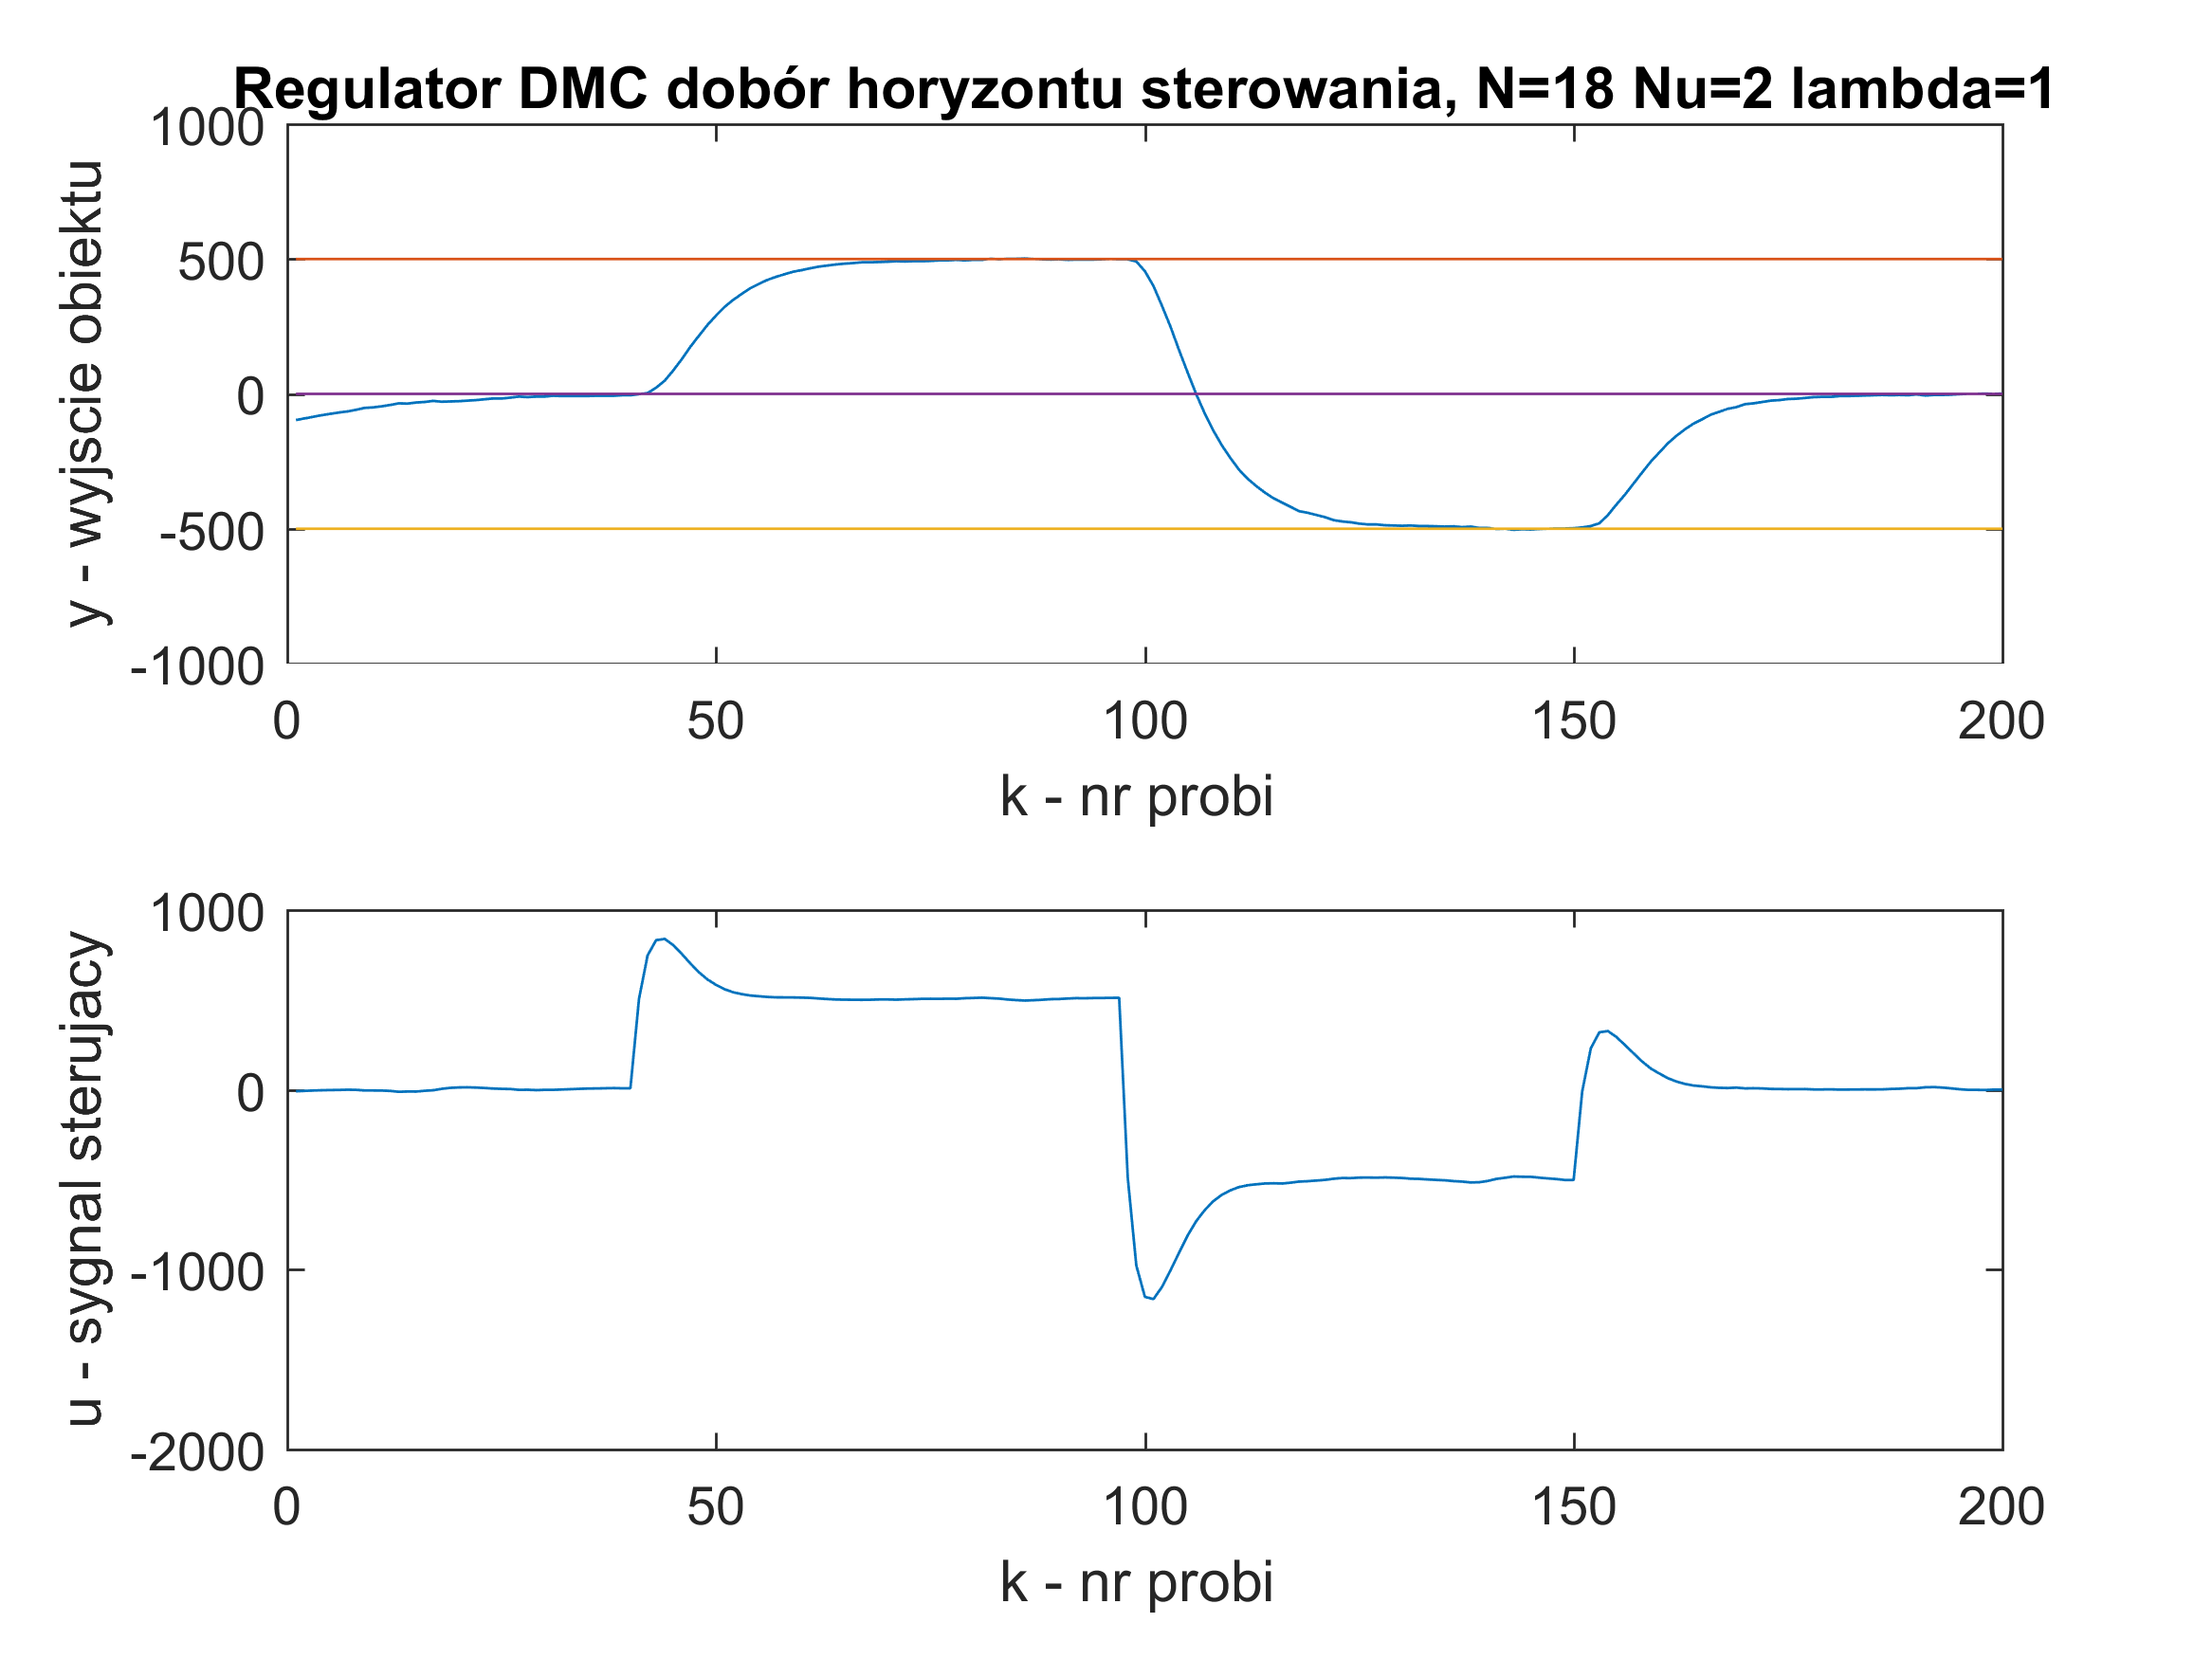
\includegraphics[width=0.9\linewidth]{DMC1821}
	\caption{Przebieg sygnałów przy $N_{u}=2$}
	\label{fig:DMC1821}
\end{figure}
Jak można zauważyć na wykresach \ref{fig:DMC1841} i \ref{fig:DMC1821}, za duże zmniejszenie horyzontu sterowania powoduje znaczące wydłużenie czasu regulacji. Pomimo tego, że sygnały zmieniają się łagodnie (co generalnie jest zaletą), czas, po jakim ustala się wyjście obiektu jest zbyt duży. Dla regulatorów z parametrem $N_{u}\geq7$ czas regulacji jest zadawalający (teoretycznie im większe $N_{u}$, tym regulator jest szybszy). Z powodu niewielkiego przeregulowania dla $N_{u}=7$ do dalszego dostrajania przyjęłyśmy taką wartość horyzontu sterowania.

\subsection{Wyznaczanie parametru $\lambda$}
Ostatnim krokiem strojenia regulatora DMC jest dobór parametru $\lambda$. Jest on odpwiedzialny za składnik kary za zmianę sygnału sterującego - im $\lambda$ jest większe, tym czas regulacji jest dłuższy i dzięki temu przebieg sygnałów jest łagodniejszy. Zmniejszenie parametru $\lambda$ powoduje skrócenie czasu regulacji kosztem wprowadzenia większych zmian w przyrostach sterowania. Przy wyznaczaniu tego parametru przyjmuje się wartości $N$ i $N_{u}$ takie, jak zostały obliczone w poprzednich krokach, czyli $N=18$ i $N_{u}=7$.
\begin{figure}[H]
	\centering
	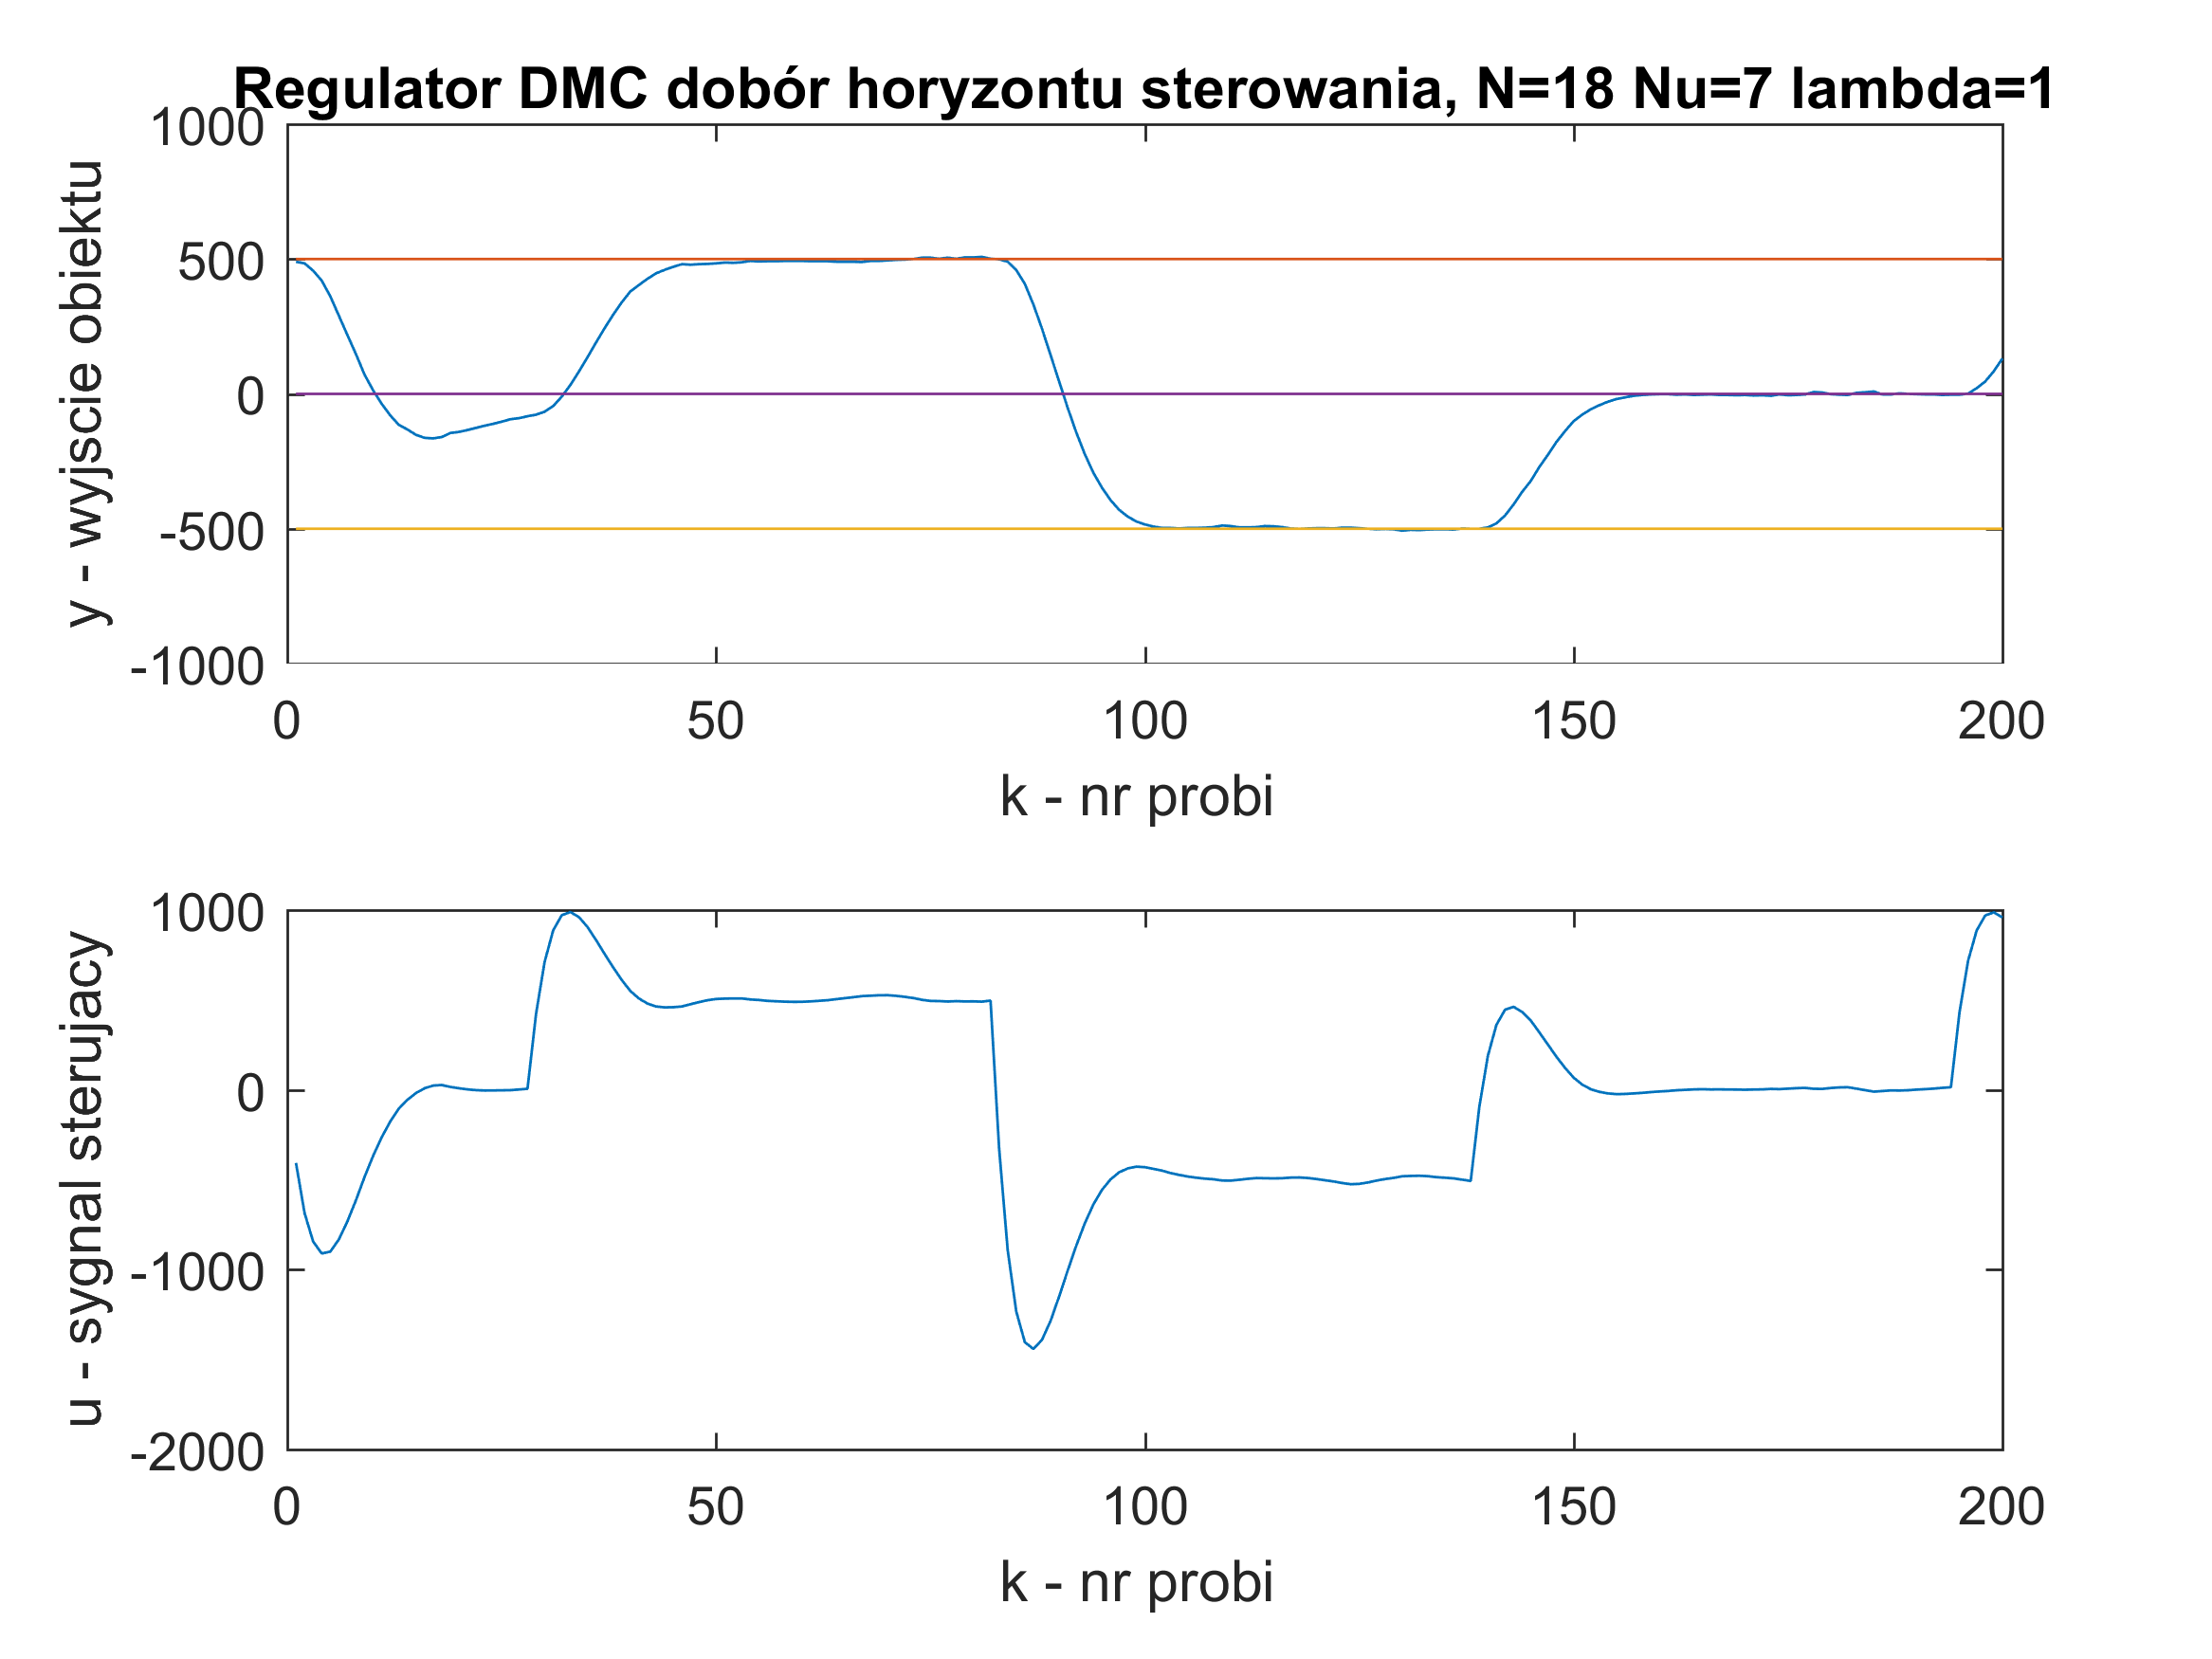
\includegraphics[width=0.9\linewidth]{DMC1871}
	\caption{Przebieg sygnałów przy $\lambda=1$}
	\label{fig:DMC1871}
\end{figure}
\begin{figure}[H]
	\centering
	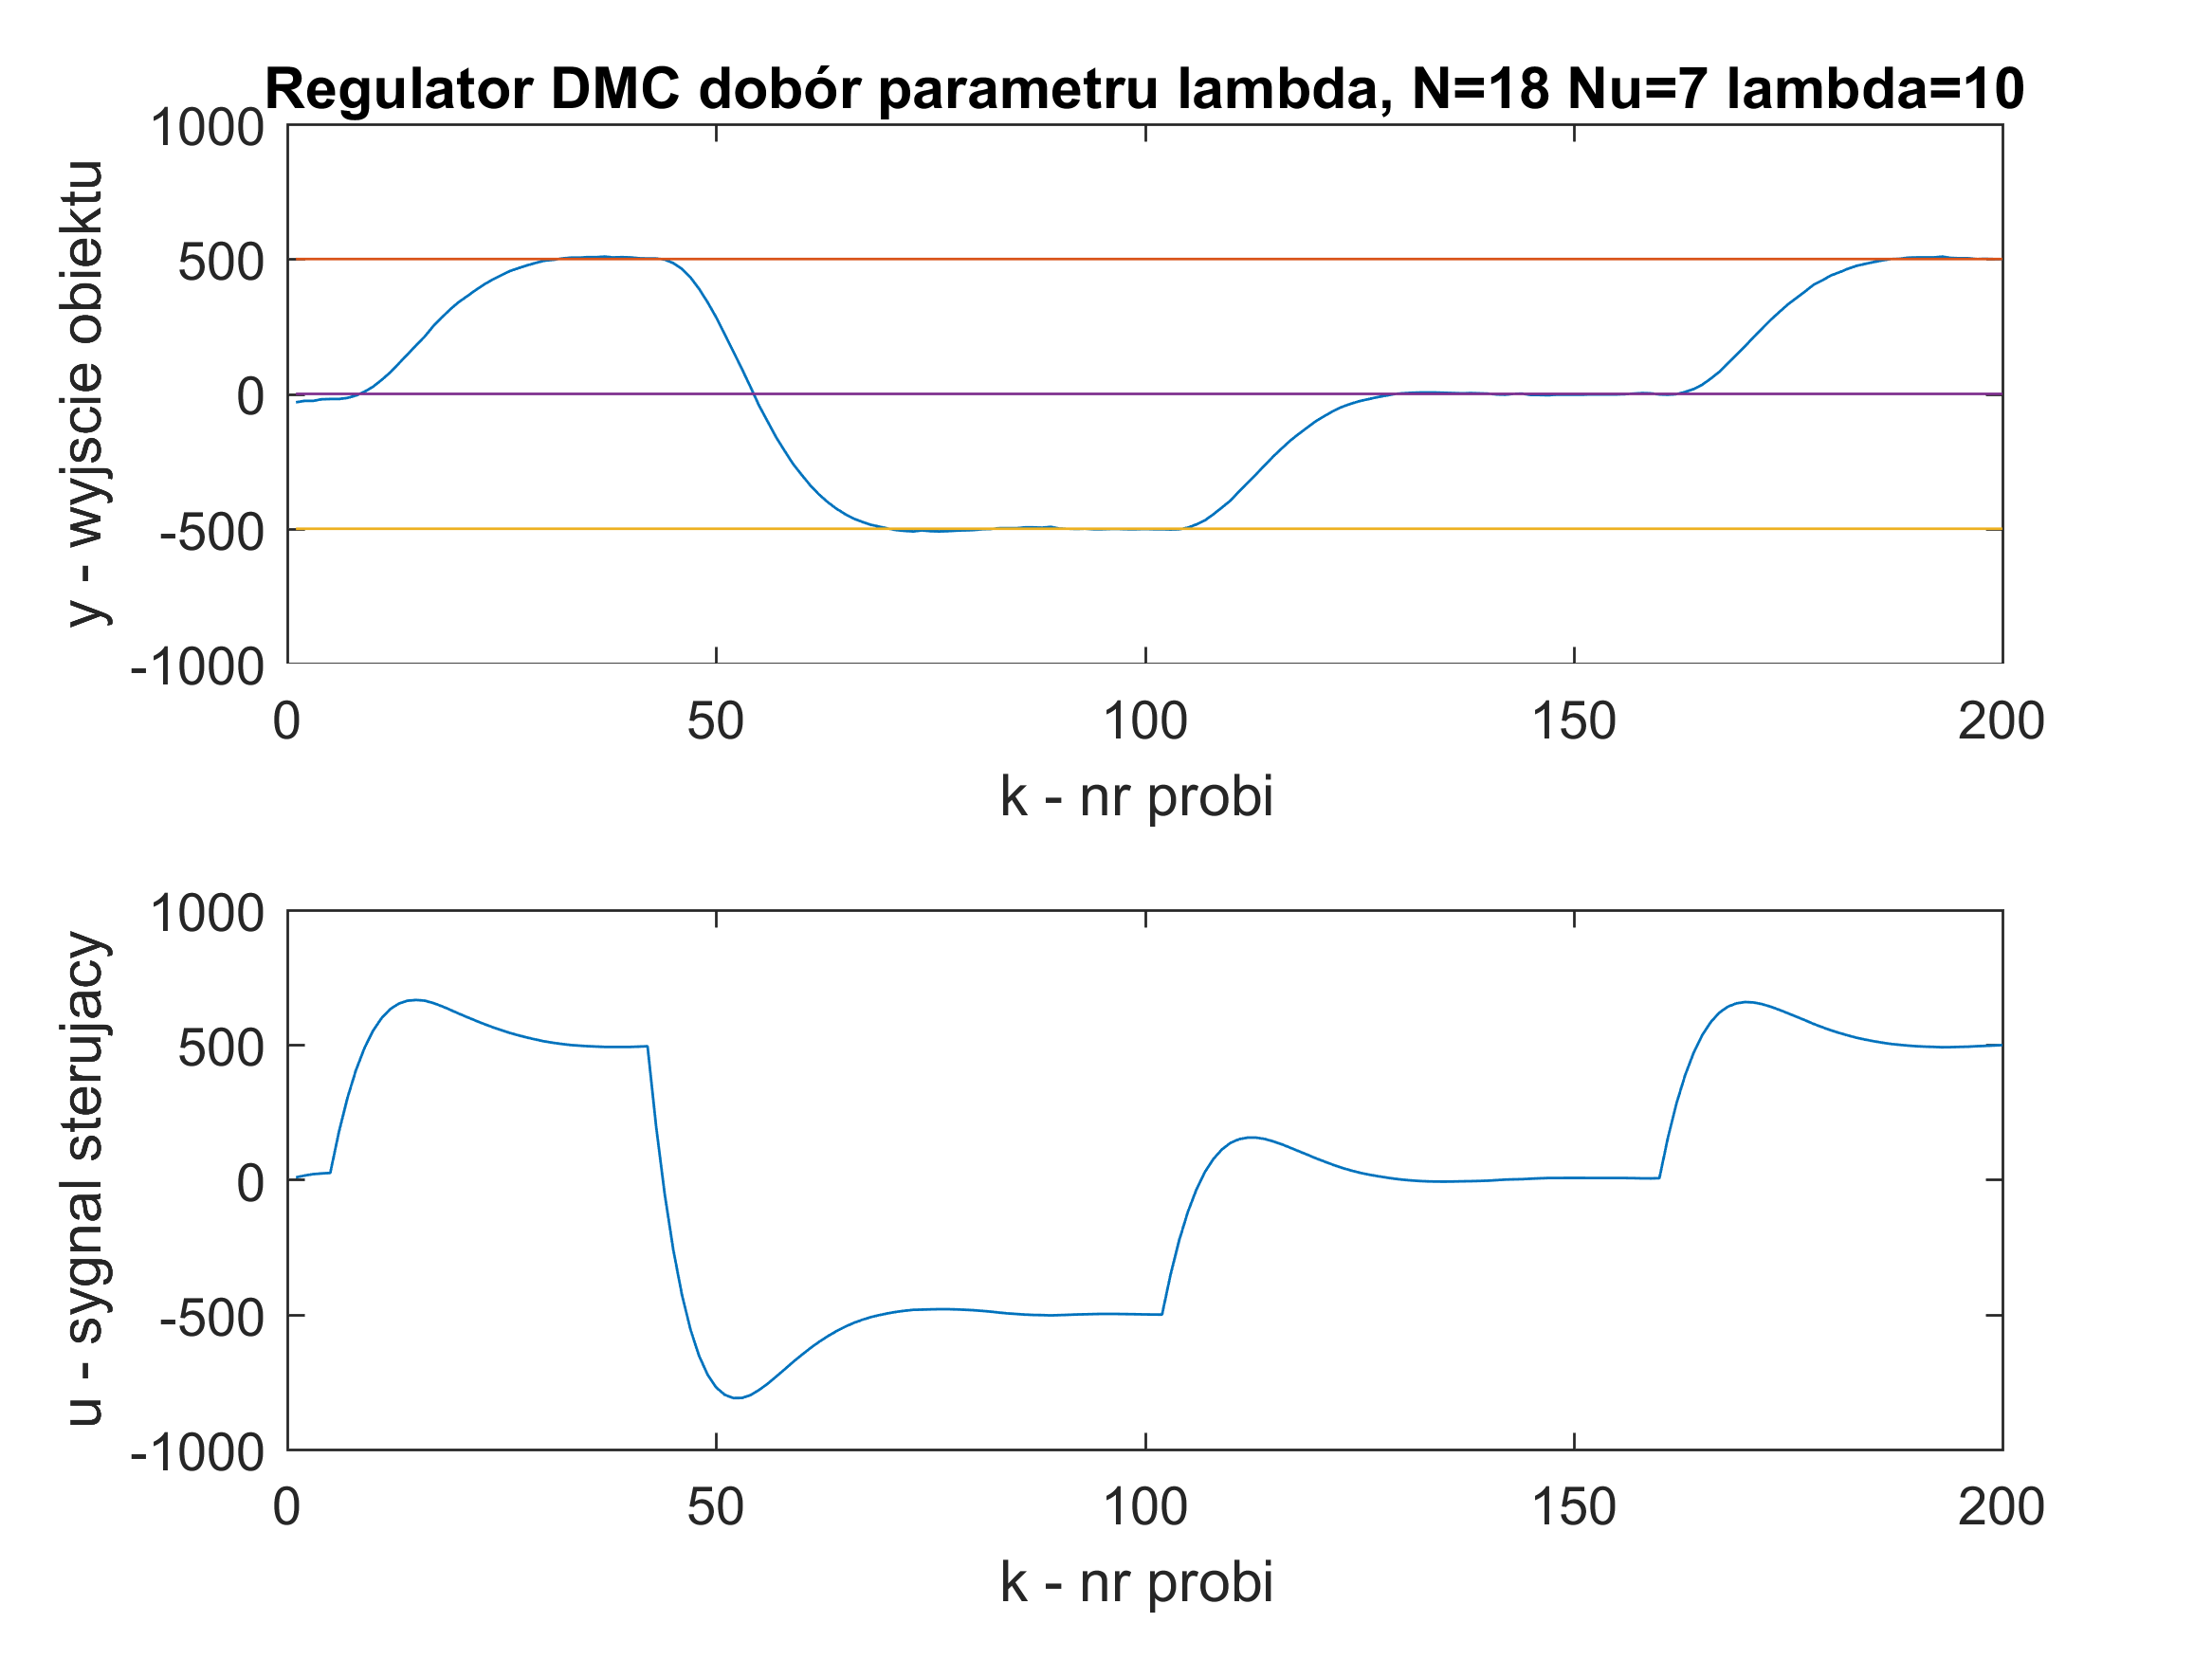
\includegraphics[width=0.9\linewidth]{DMC18710}
	\caption{Przebieg sygnałów przy $\lambda=10$}
	\label{fig:DMC18710}
\end{figure}
\begin{figure}[H]
	\centering
	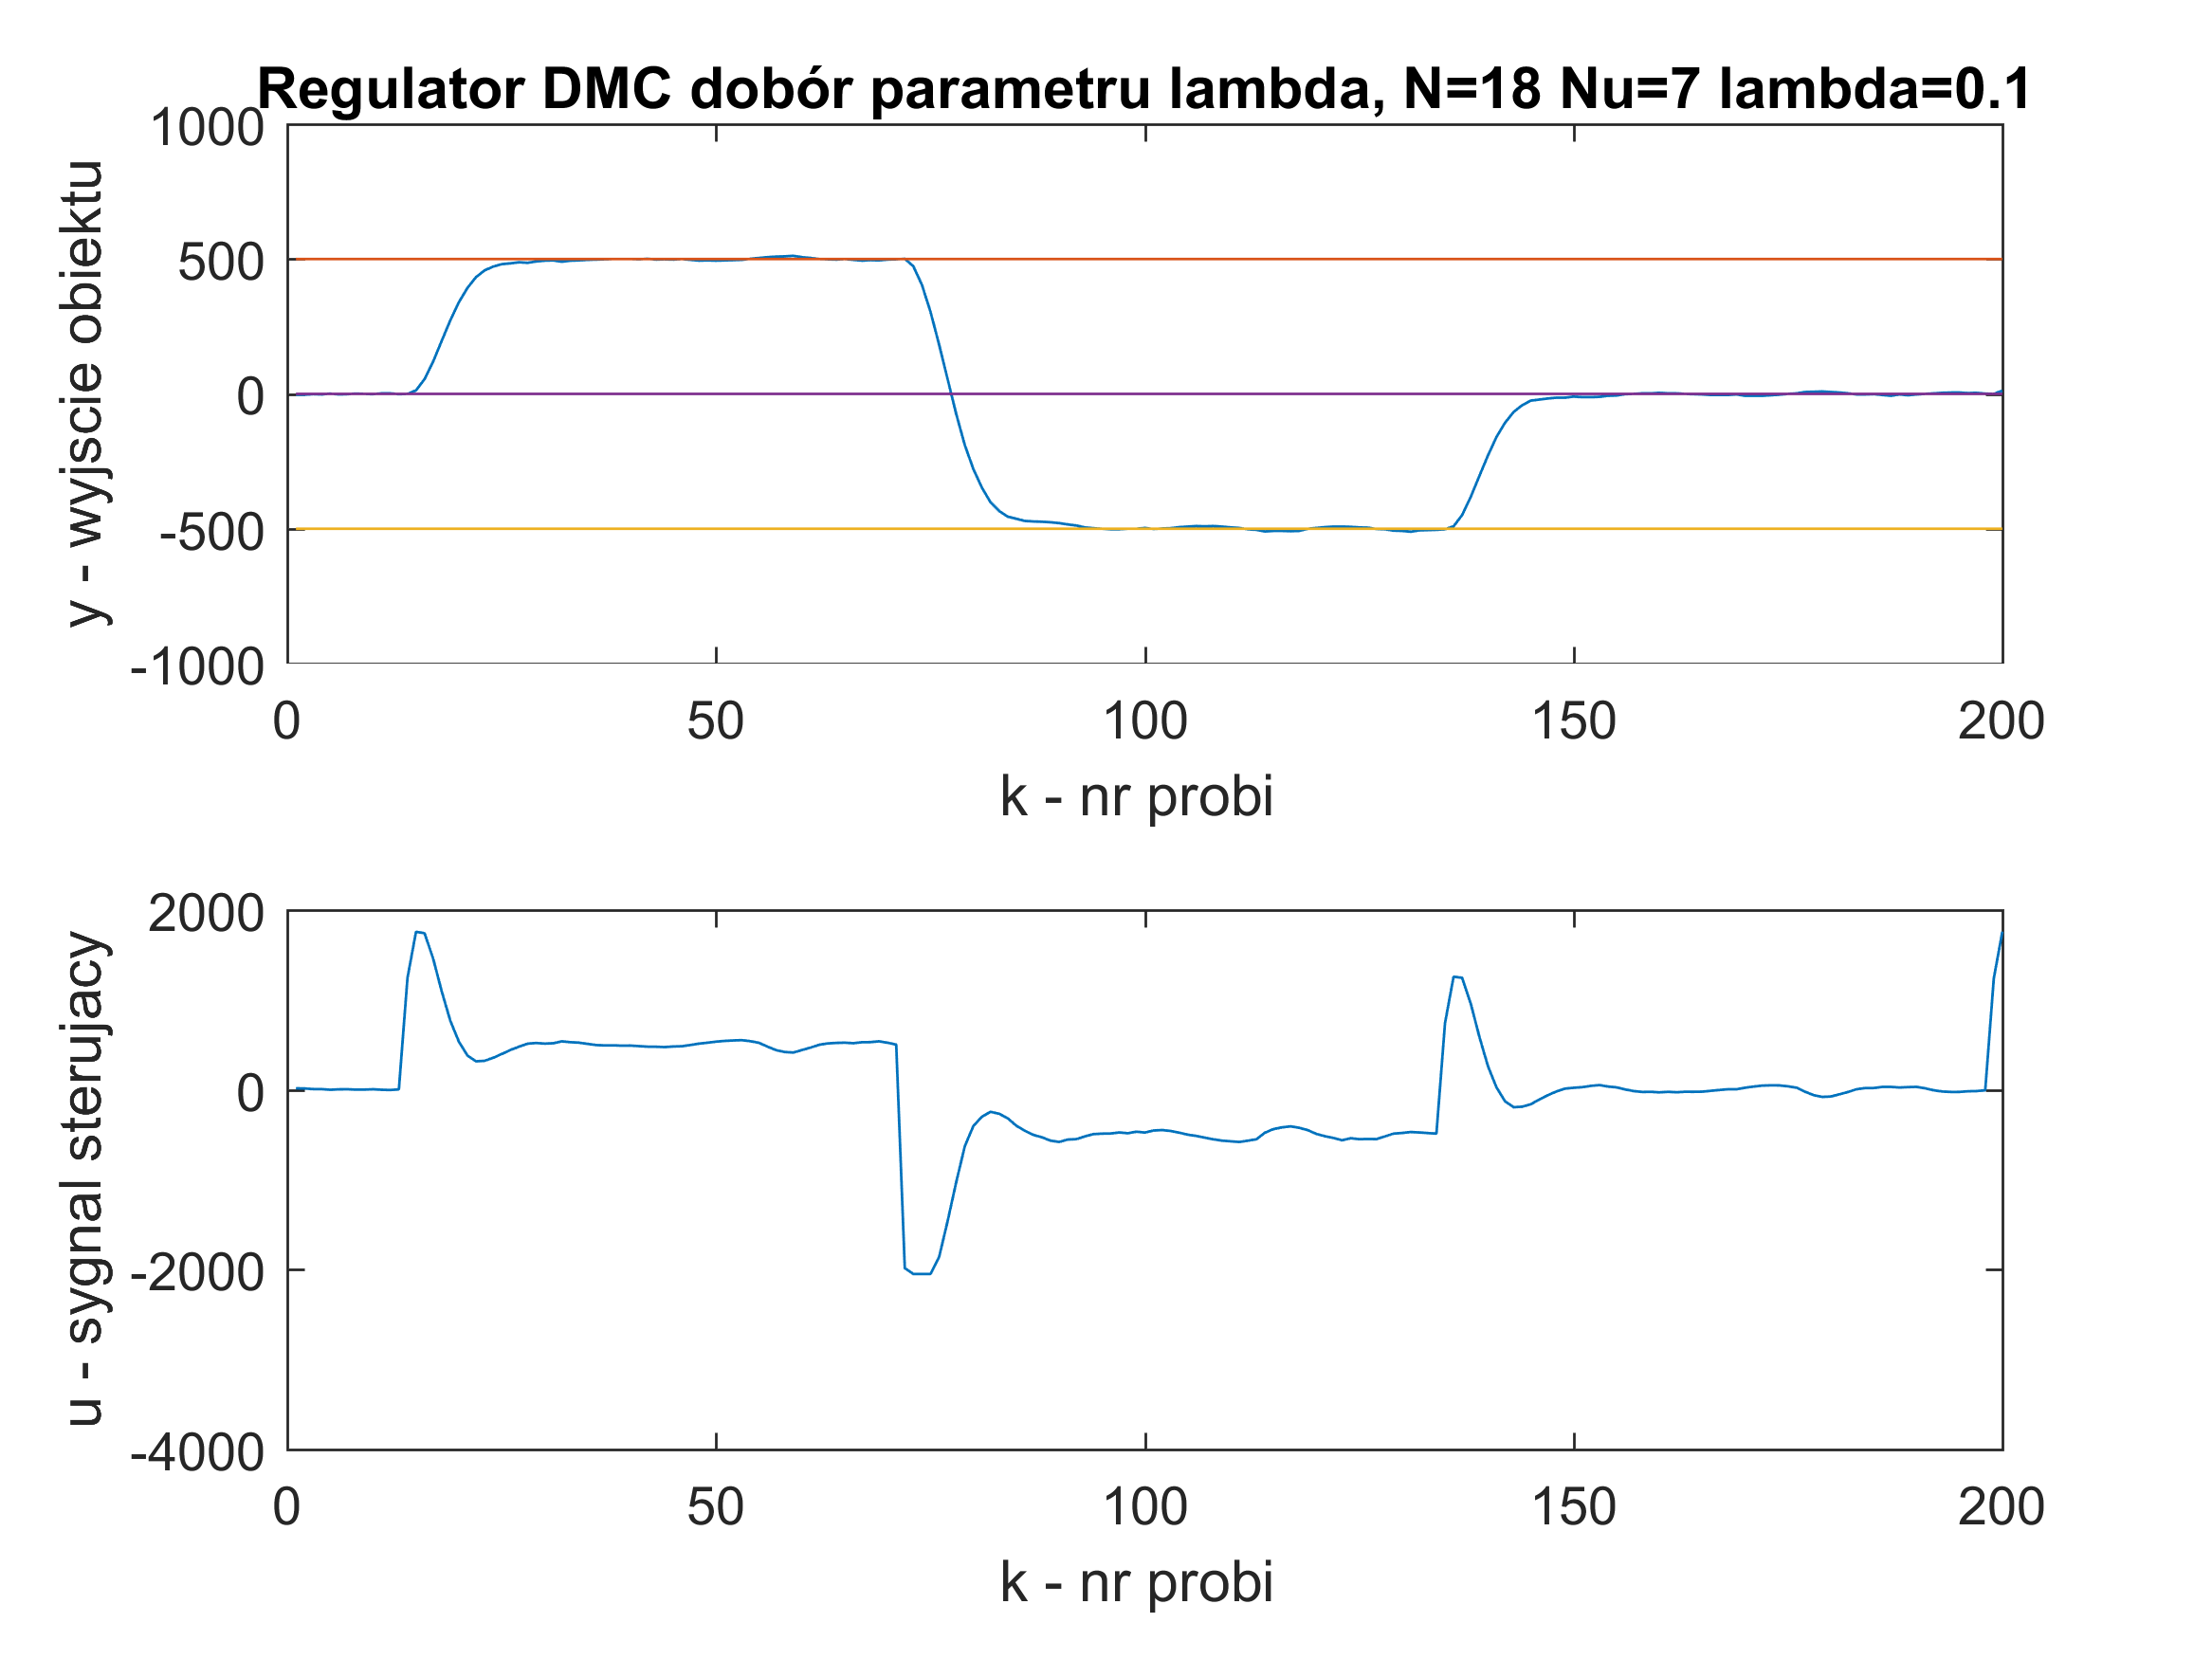
\includegraphics[width=0.9\linewidth]{DMC18710000000}
	\caption{Przebieg sygnałów przy $\lambda=0,1$}
	\label{fig:DMC18710000000}
\end{figure}
\begin{figure}[H]
	\centering
	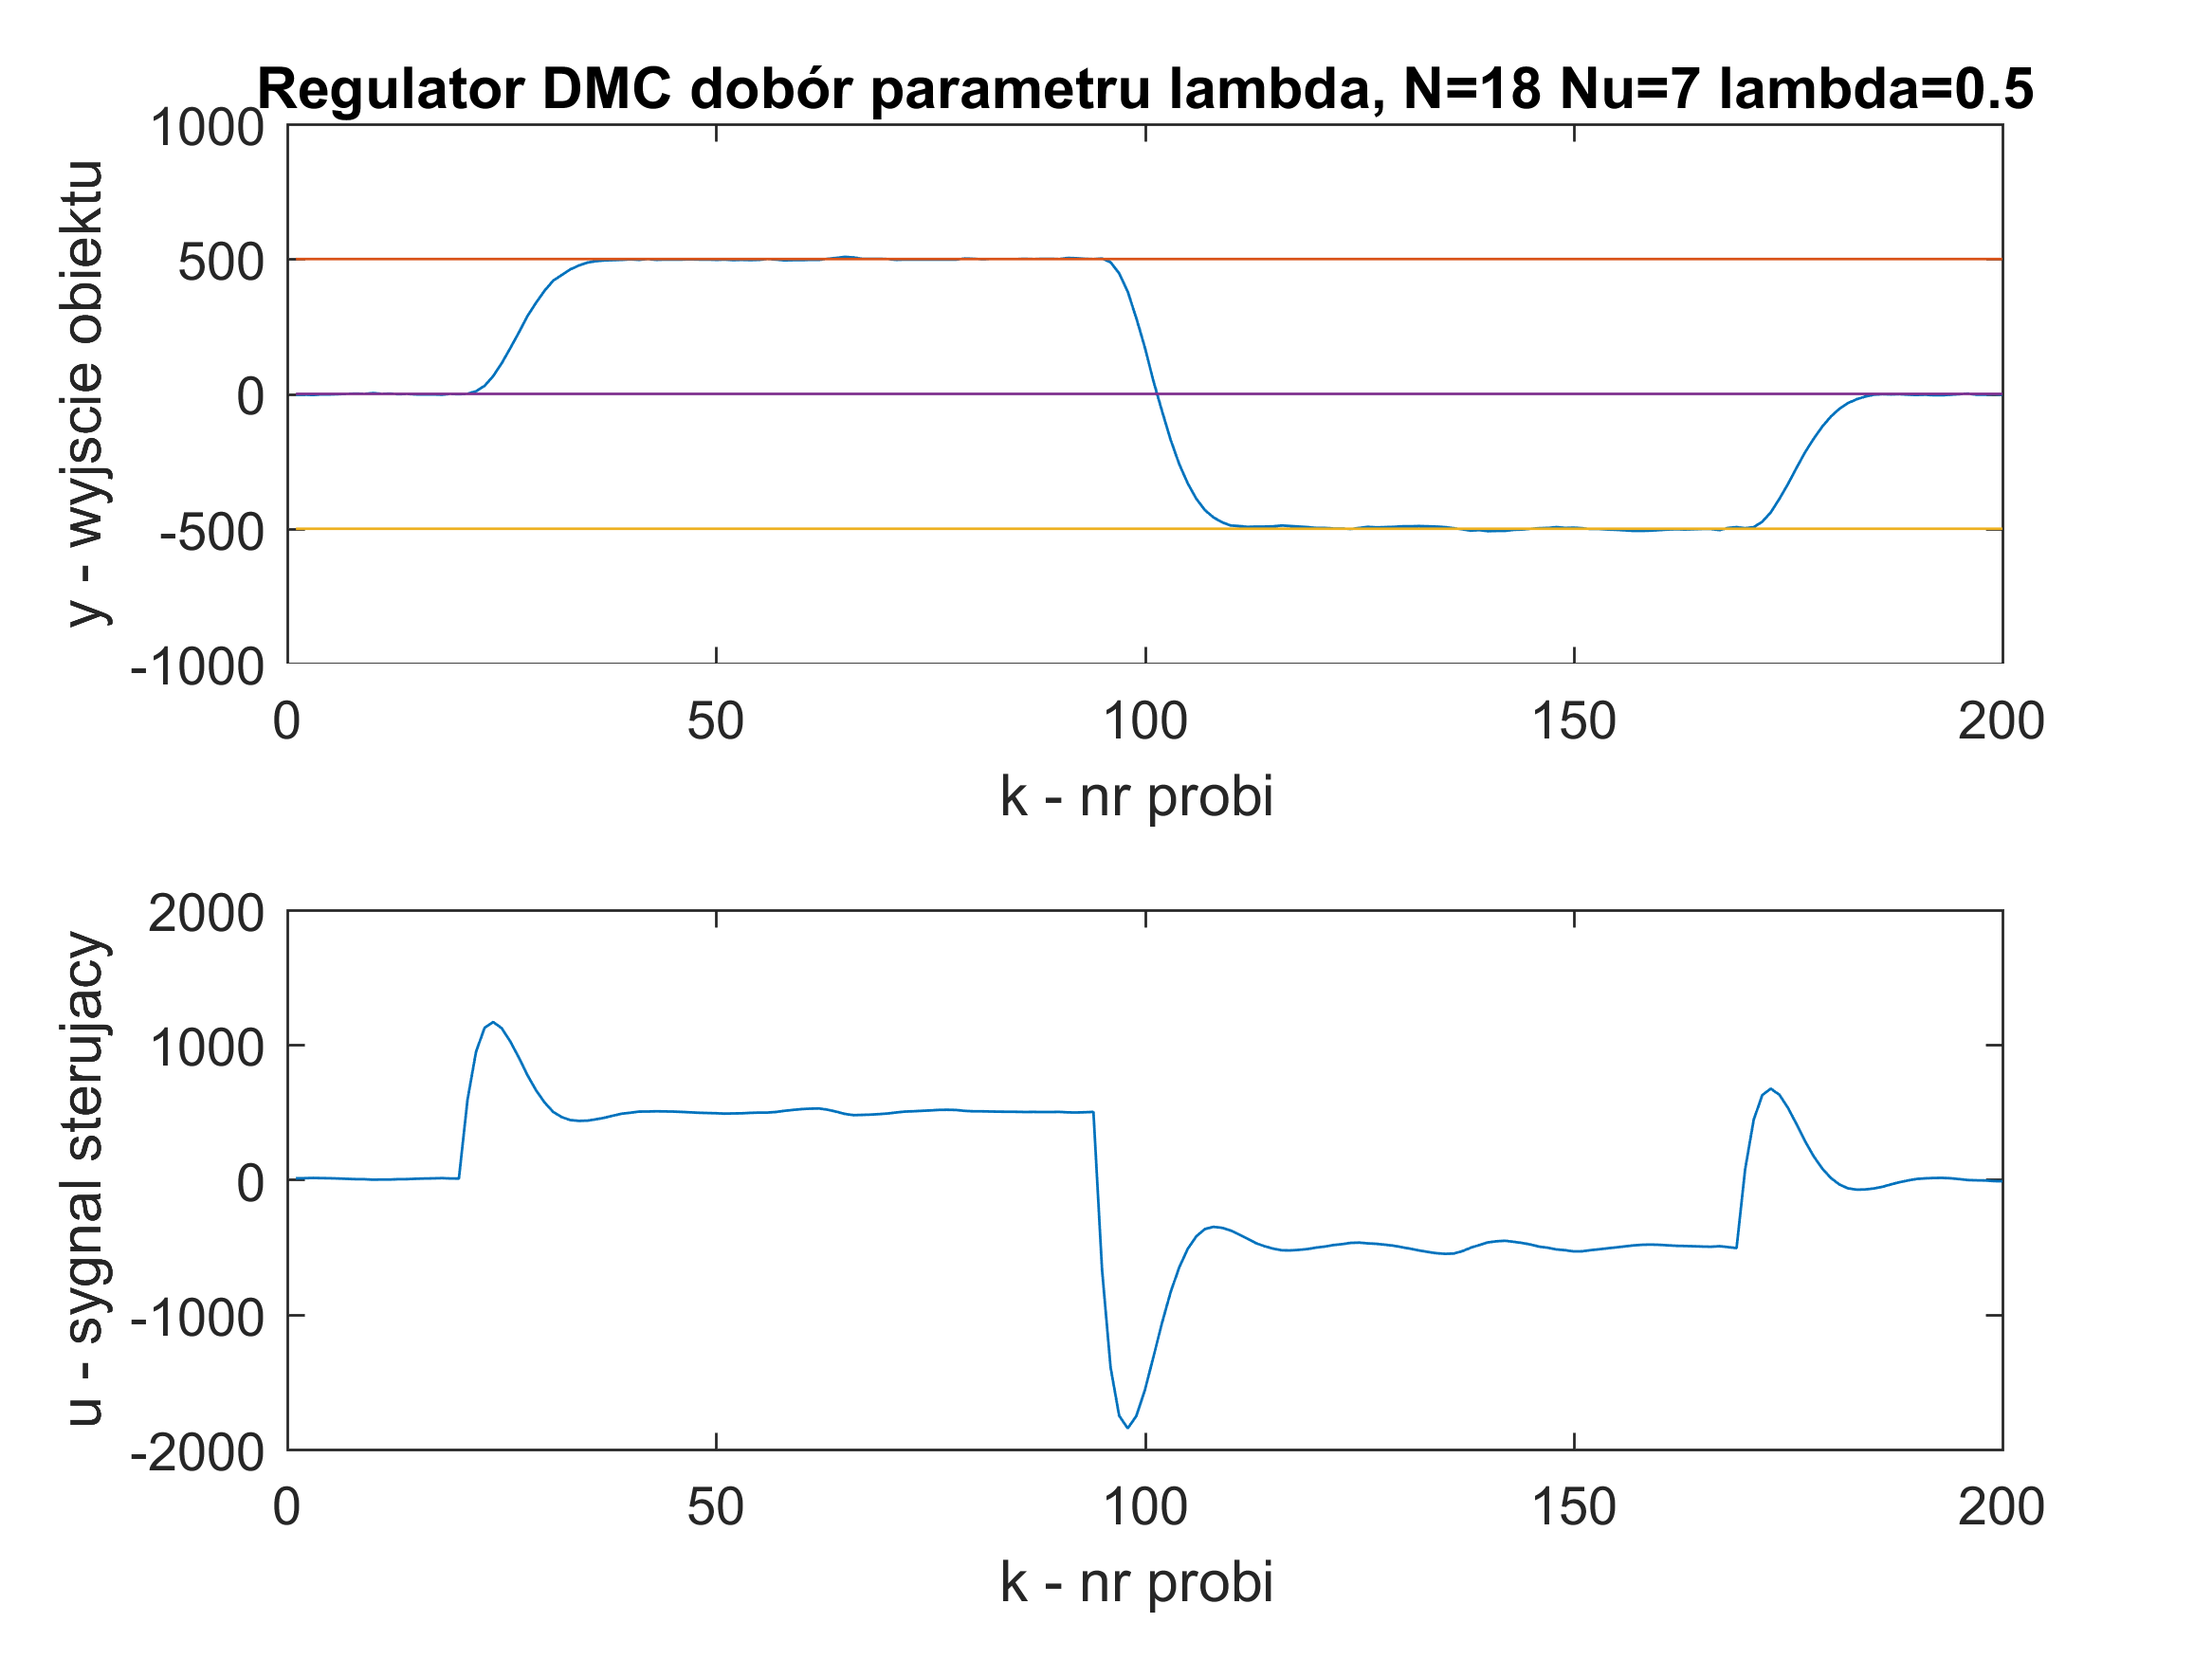
\includegraphics[width=0.9\linewidth]{DMC18750000000}
	\caption{Przebieg sygnałów przy $\lambda=0,5$}
	\label{fig:DMC18750000000}
\end{figure}
\begin{figure}[H]
	\centering
	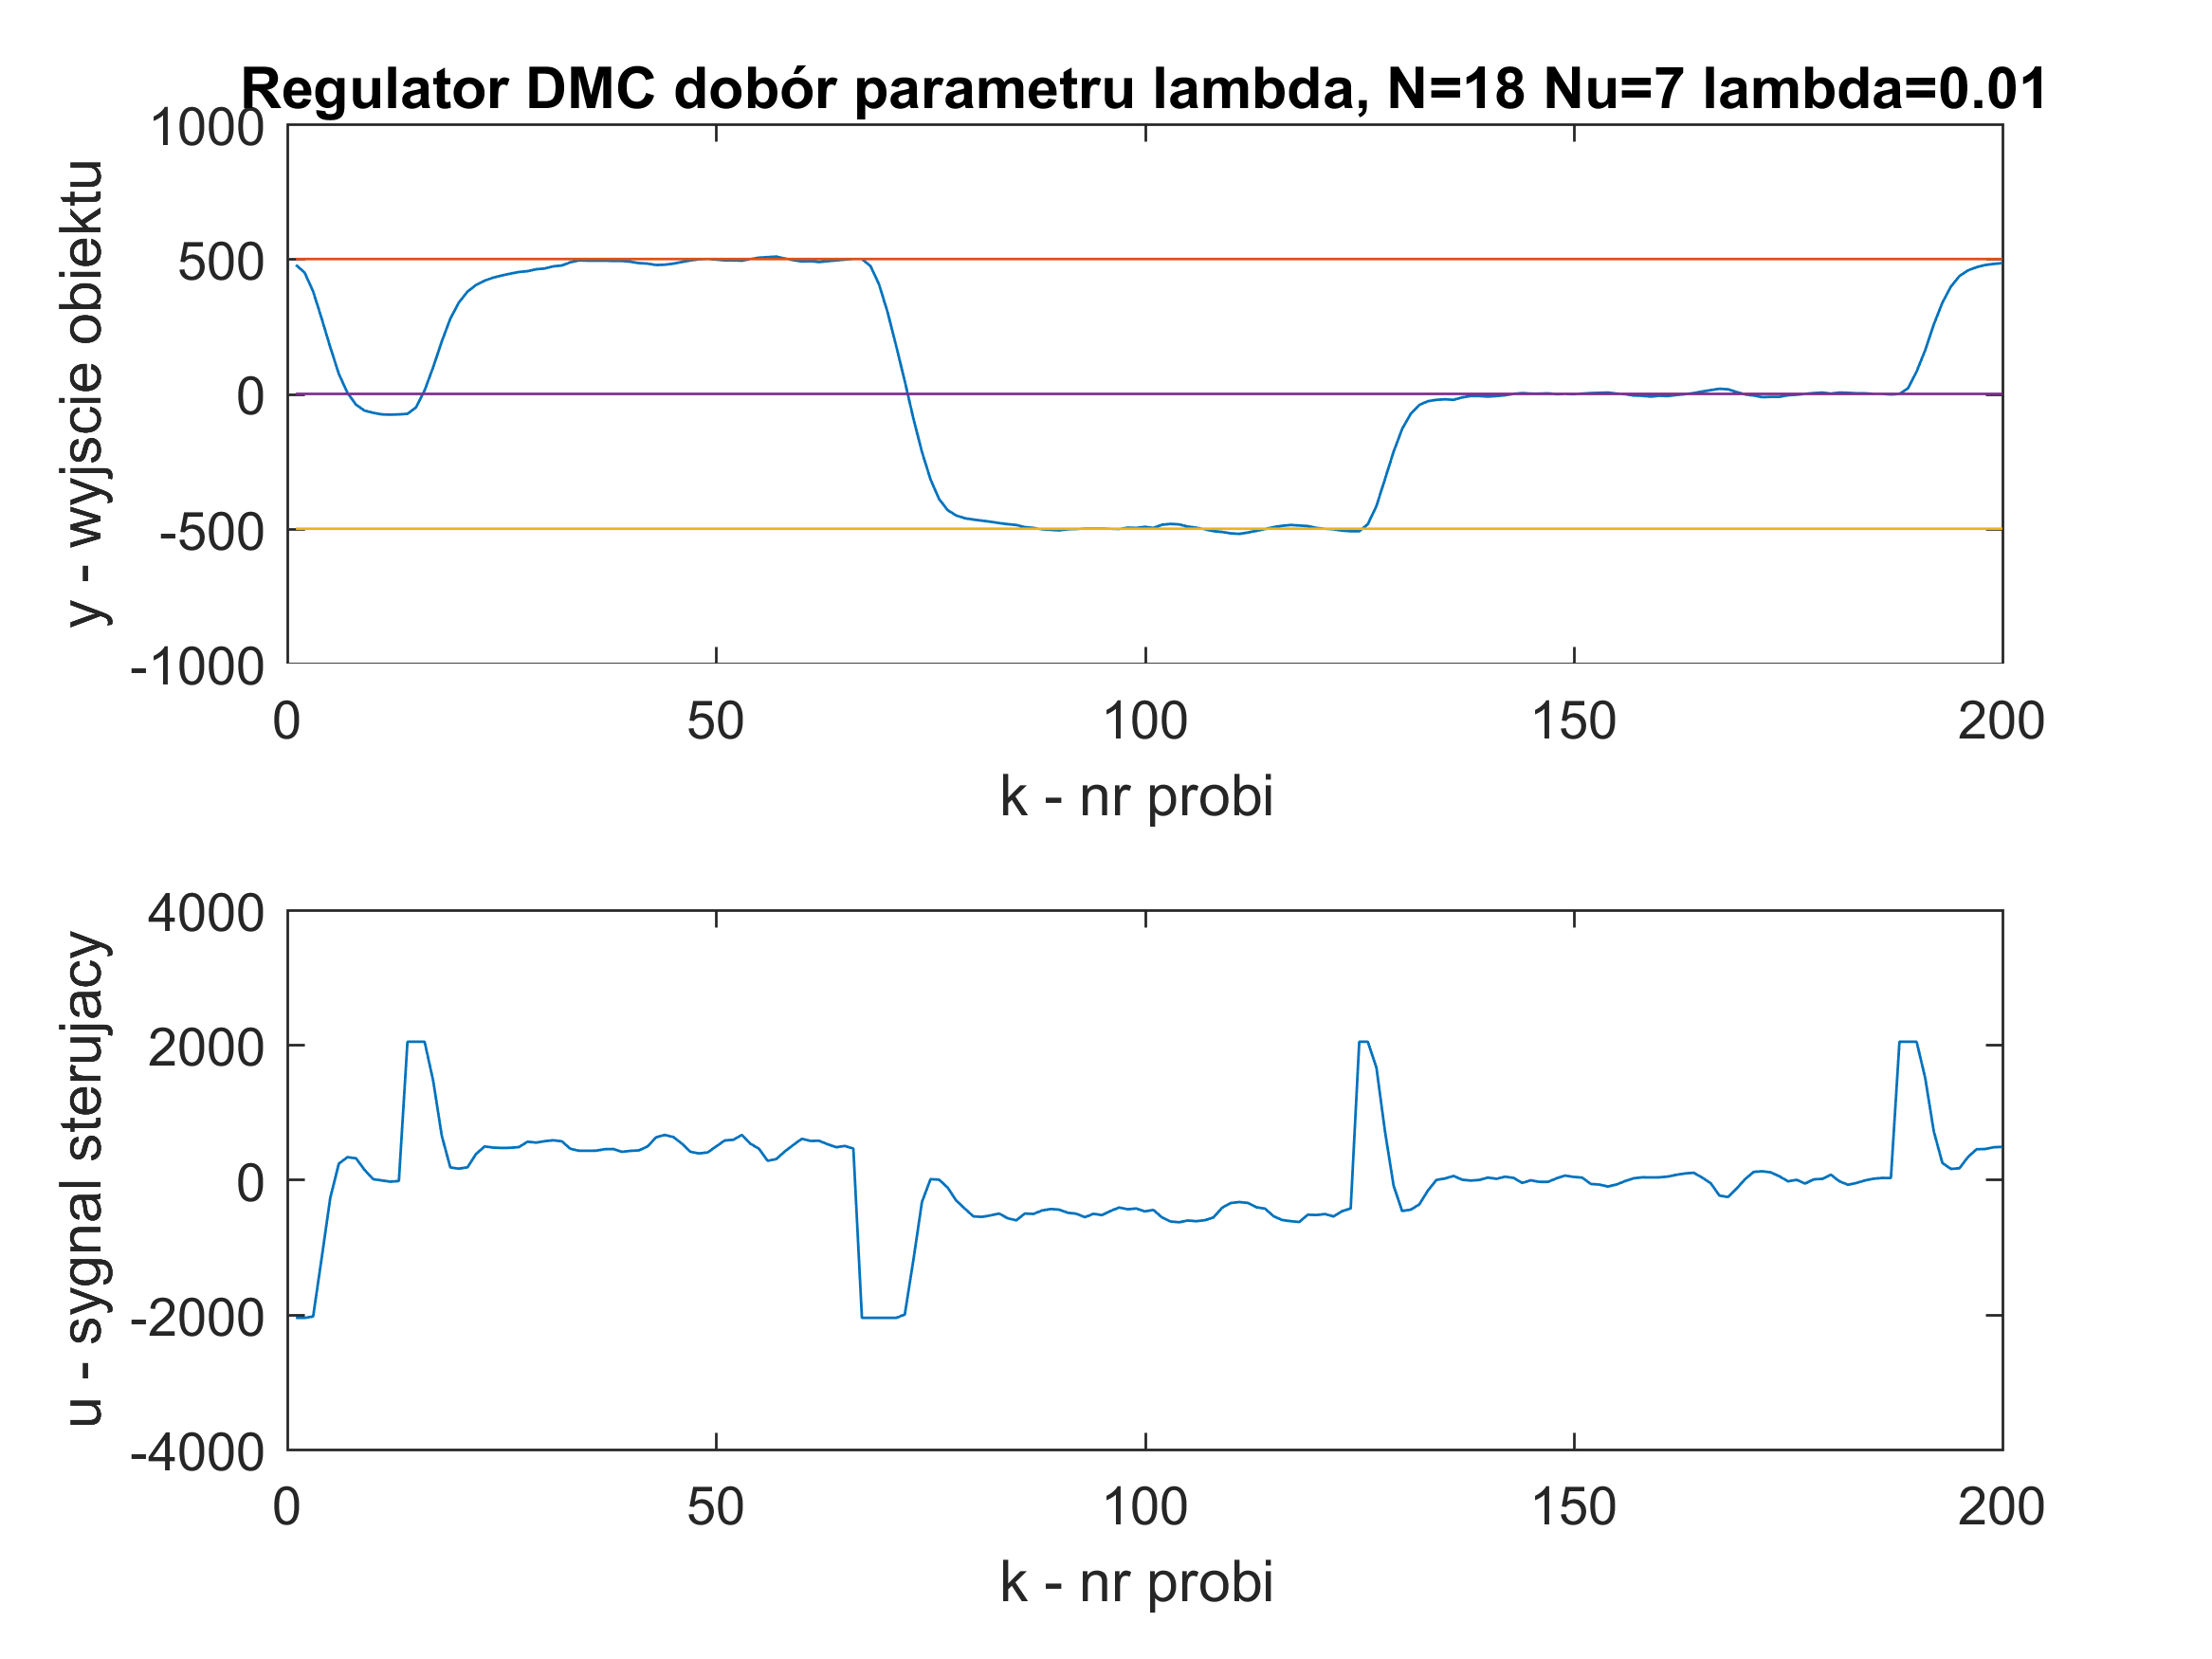
\includegraphics[width=0.9\linewidth]{DMC1871000000}
	\caption{Przebieg sygnałów przy $\lambda=0,01$}
	\label{fig:DMC1871000000}
\end{figure}
Zgodnie z oczekiwaniami, jak można zauważyć na wykresie \ref{fig:DMC18710} zwiększenie parametru $\lambda$ powoduje wydłużenie czasu regulacji i sprawia, że przebieg sygnałów jest łagodniejszy. W przypadku danego obiektu nie przynosi to korzyści. Z wykresu \ref{fig:DMC18710000000} i \ref{fig:DMC1871000000} wynika, że zmniejszenie parametru $\lambda$ oprócz skrócenia czasu regulacji zwiększyło amplitudę oscylacji sygnałów. Kompromis pomiędzy szybkim czasem regulacji a niewielkimi oscylacjami sygnałów został osiągnięty dla parametru $\lambda=0,5$.

Ostatecznie wybrane nastawy regulatora DMC:
\[N=18, N_{u}=7, \lambda=0,5\].

\begin{figure}[H]
	\centering
	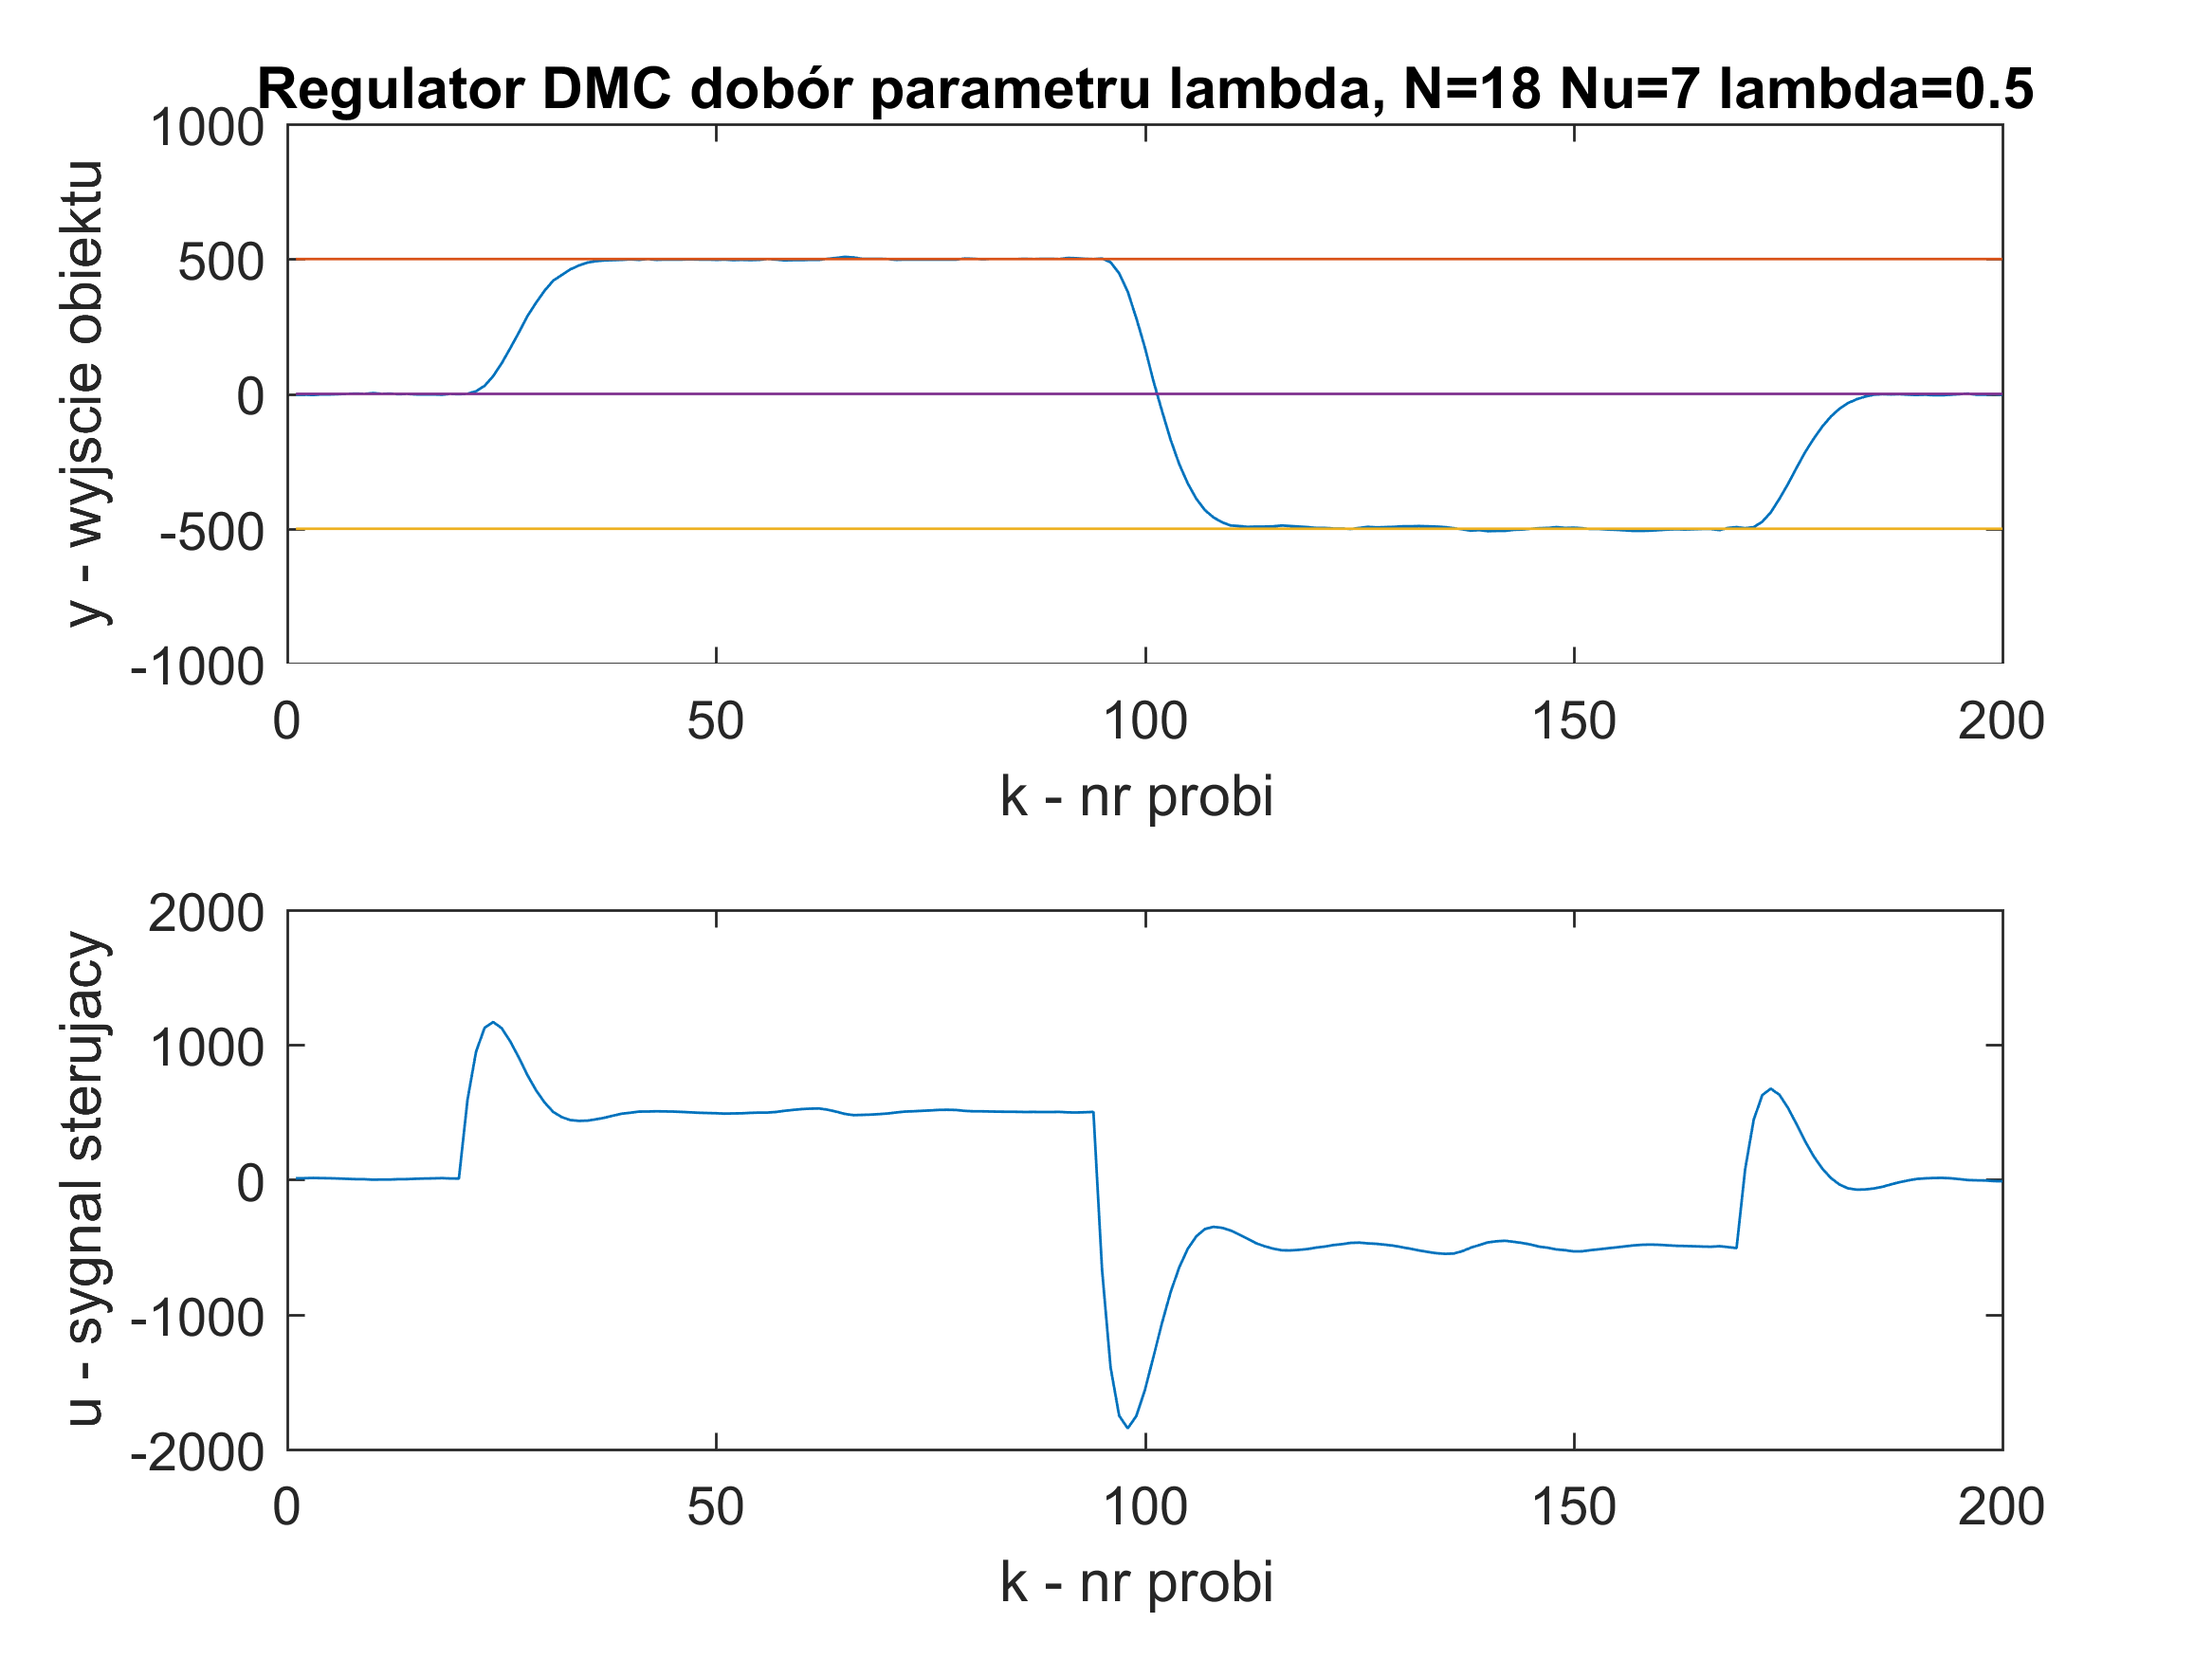
\includegraphics[width=0.9\linewidth]{DMC18750000000}
	\caption{Ostatecznie wybrany regulator DMC}
	\label{fig:DMCost}
\end{figure}

\section{Porównanie najlepszej realizacji algorytmu PID i DMC}

Regulatory PID i DMC zostaną porównane pod kątem odporności na zakłócenia, przeregulowania, czasu ustalenia i oscylacji.

W punkcie \ref{porownaj} zostały przedstawione używane wzory na przeregulowanie i czas ustalenia, które będą używane w poniższych sekcjach.

\subsection{Odporność na zakłócenia}
Odporność na zakłócenia została sprawdzona poprzez wcisnięcie przycisku na płytce z obiektem symulowanym.

Wyniki tego testu widać na rysunkach: \ref{fig:pidzaklocenia} - dla regulatora PID i  \ref{fig:dmc001zakl}, \ref{fig:dmc05zakl} - dla regulatora DMC z różnymi wartościami $\lambda$.

Dla regulatora PID sygnał sterujący zmienia się w sposób gwałtowny i dociera do ograniczeń (wartość -2000). Wartość sygnału sterujacego dla regulatora DMC jest ograniczona. Wynika to z brania pod uwagę zmiany wartości sterowania przy wyliczaniu wskaźnika jakości. W zależności od wybranego lambda sygnał jest mniej gwałtowny i ma mniejszą amplitudę (dla $\lambda = 0,5$) lub bardziej gwałtowny i z występującą większą amplitudą (dla $\lambda = 0,01$). Zgadza się to wskaźnikiem jakości - im mniejsza lambda, tym mniejsza kara za zmianę sygnału sterującego. Nadal jednak, dla niezerowej lambdy, sygnał sterujący algorytmu DMC jest mniej gwałtowny i ma mniejszą amplpitudę od sygnału sterujacego regulatora PID.

Z uwagi na to, że regulator PID ma większą wartość i gwałtowniejszy wzrost sygnału sterującego przy wystapieniu zakłócenia, regulator PID szybciej niweluje to zakłócenie. Wynika to także z faktu, że regulator PID przy wyliczaniu sterowania bierze pod uwagę sterowanie z 3 ostatnich chwil czasu. Regulator DMC ze względu na ograniczenie na sygnał sterujący oraz tego, że bierze pod uwagę jedynie wartość sterowania z poprzedniej chwili czasu, wolniej radzi sobie z niwelacją zakłócenia. 

Szybkość niwelacji zakłócenia wpływa na amplitudę sygnału wyjściowego przy wystąpieniu zakłócenia. Regulator PID sprawniej niweluje zakłócenie, więc amplituda sygnału nie zdąży osiągnać tak dużej wartości. Amplituda sygnału wyjściowego dla regulatora DMC będzie większa, ponieważ gorzej radzi sobie on z niwelacją zakłócenia. 

\begin{figure}[H]
	\centering
	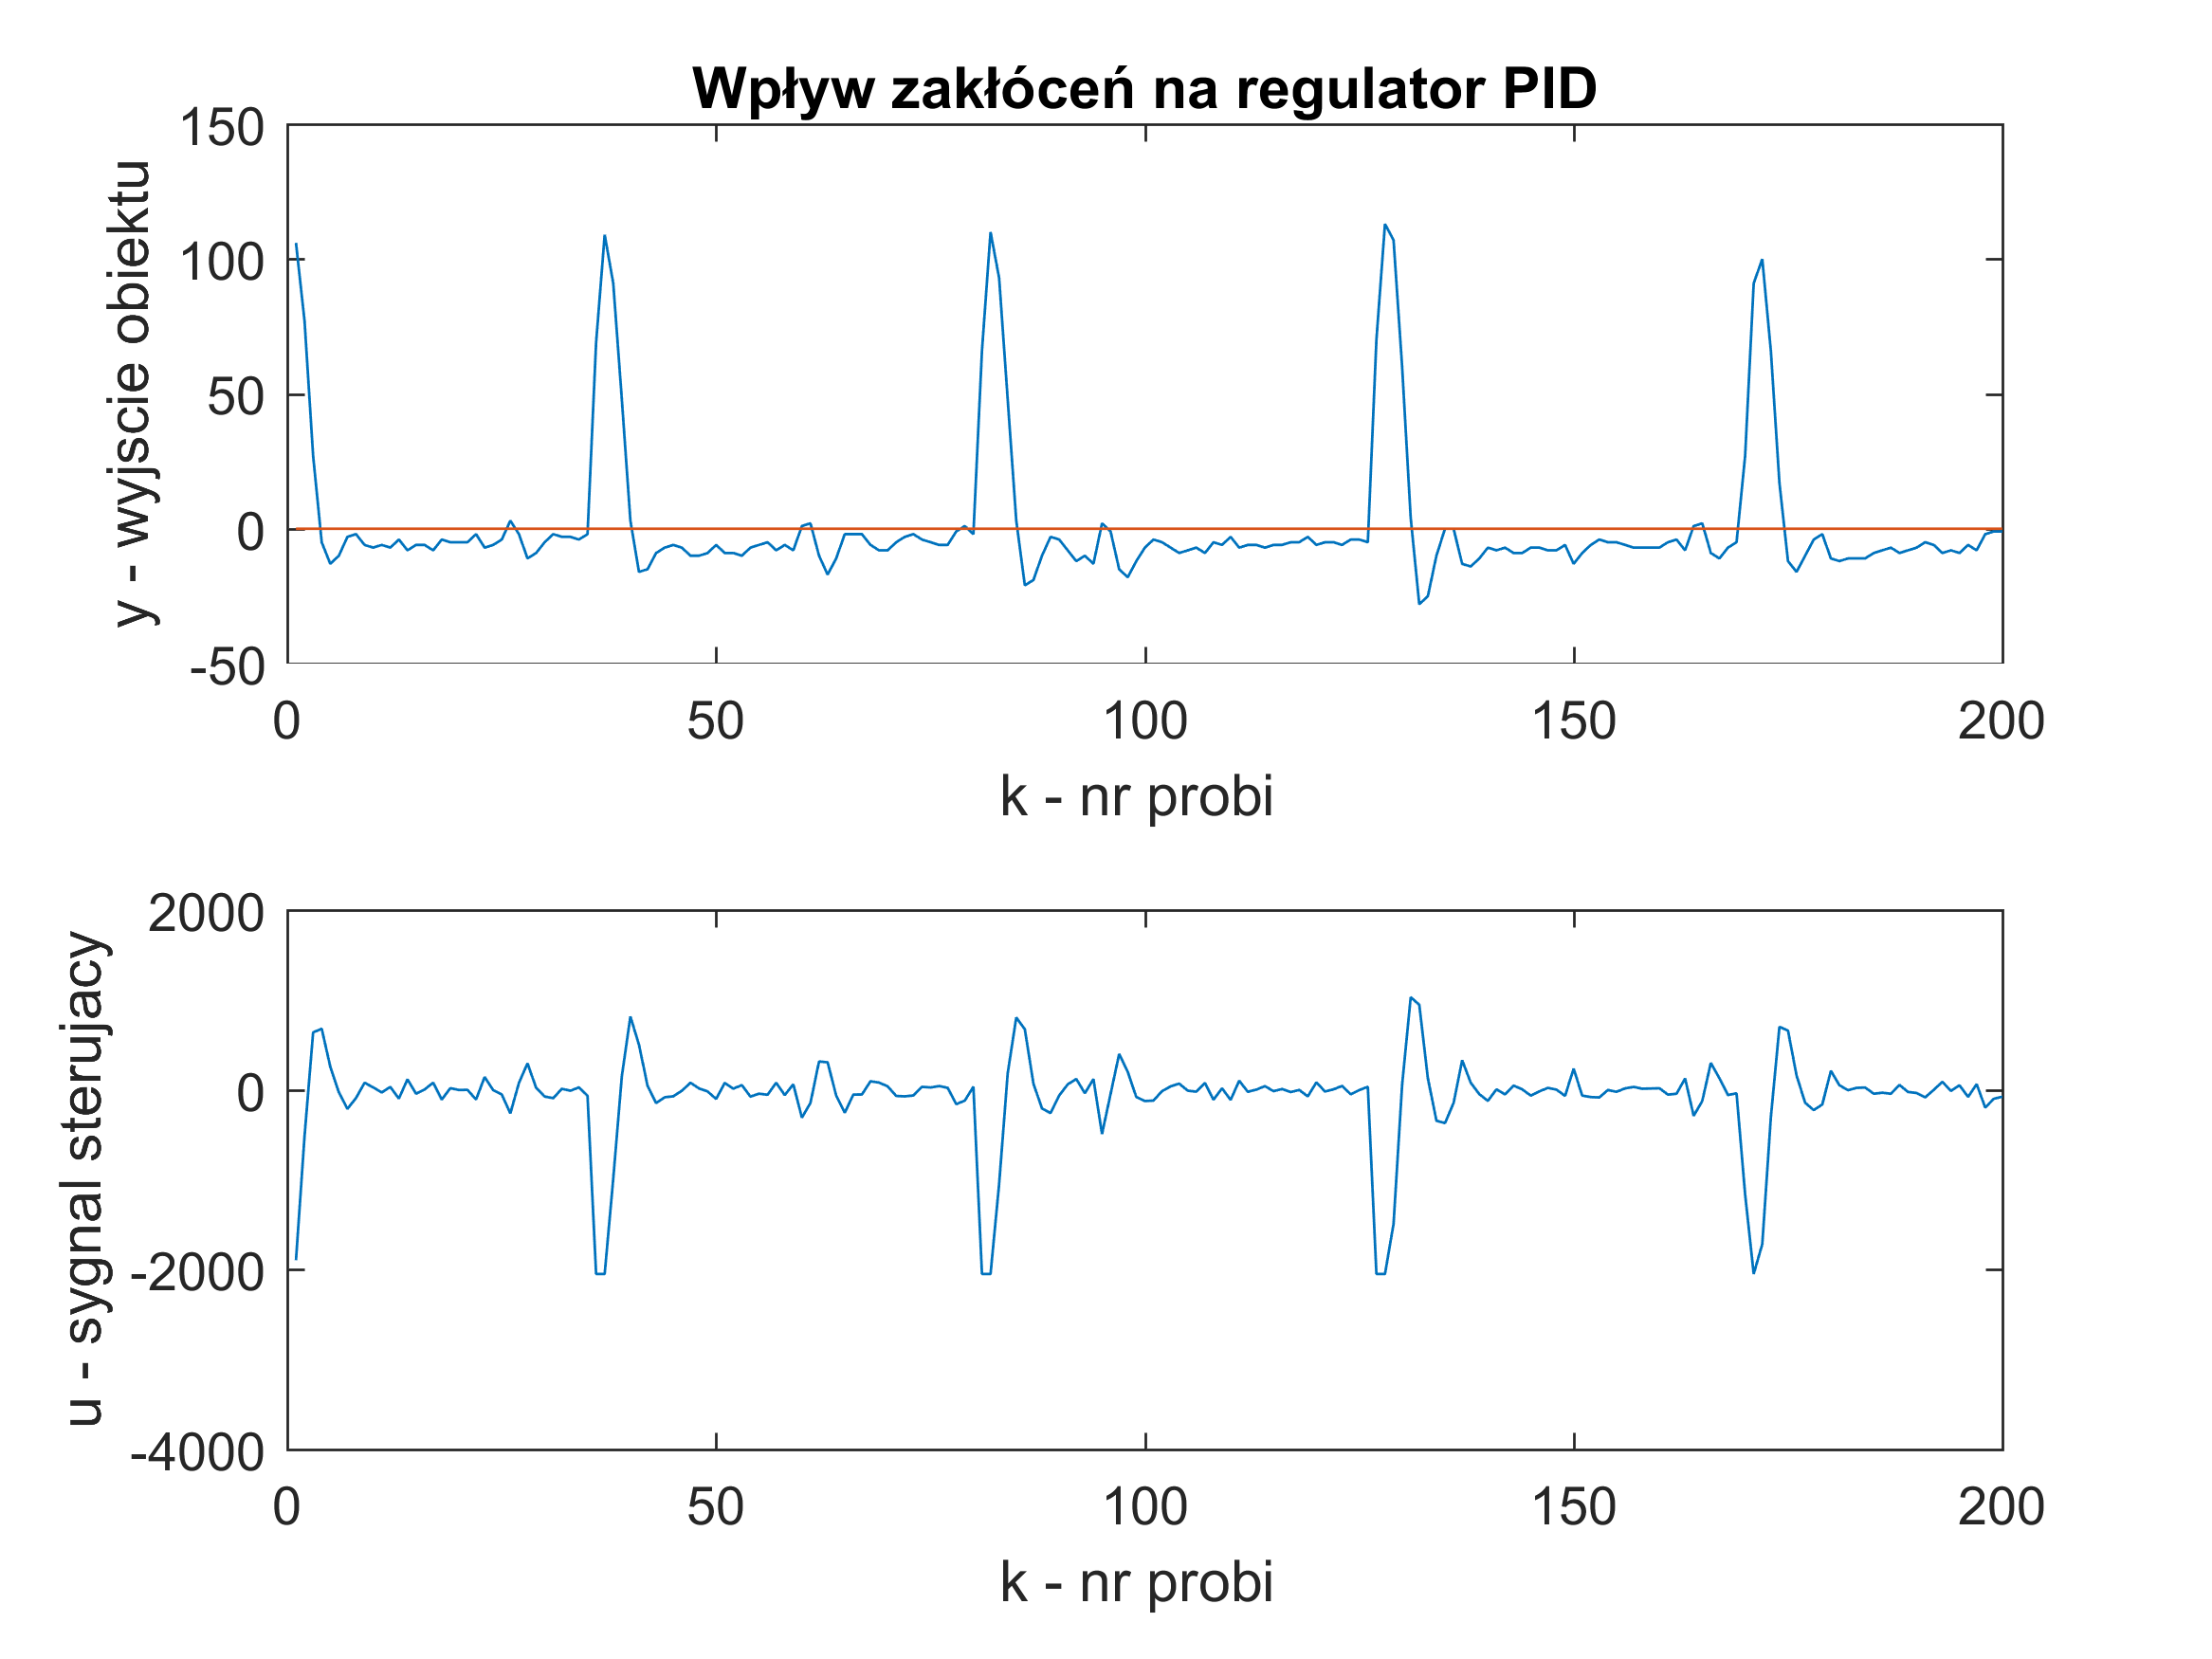
\includegraphics[width=0.9\linewidth]{pidzaklocenia}
	\caption{Ocena regulatora PID wyznaczonego metodą inżynierską: $K=14, T_{i}=1,8, T_{d}=0,08$}
	\label{fig:pidzaklocenia}
\end{figure}

\begin{figure}[H]
	\centering
	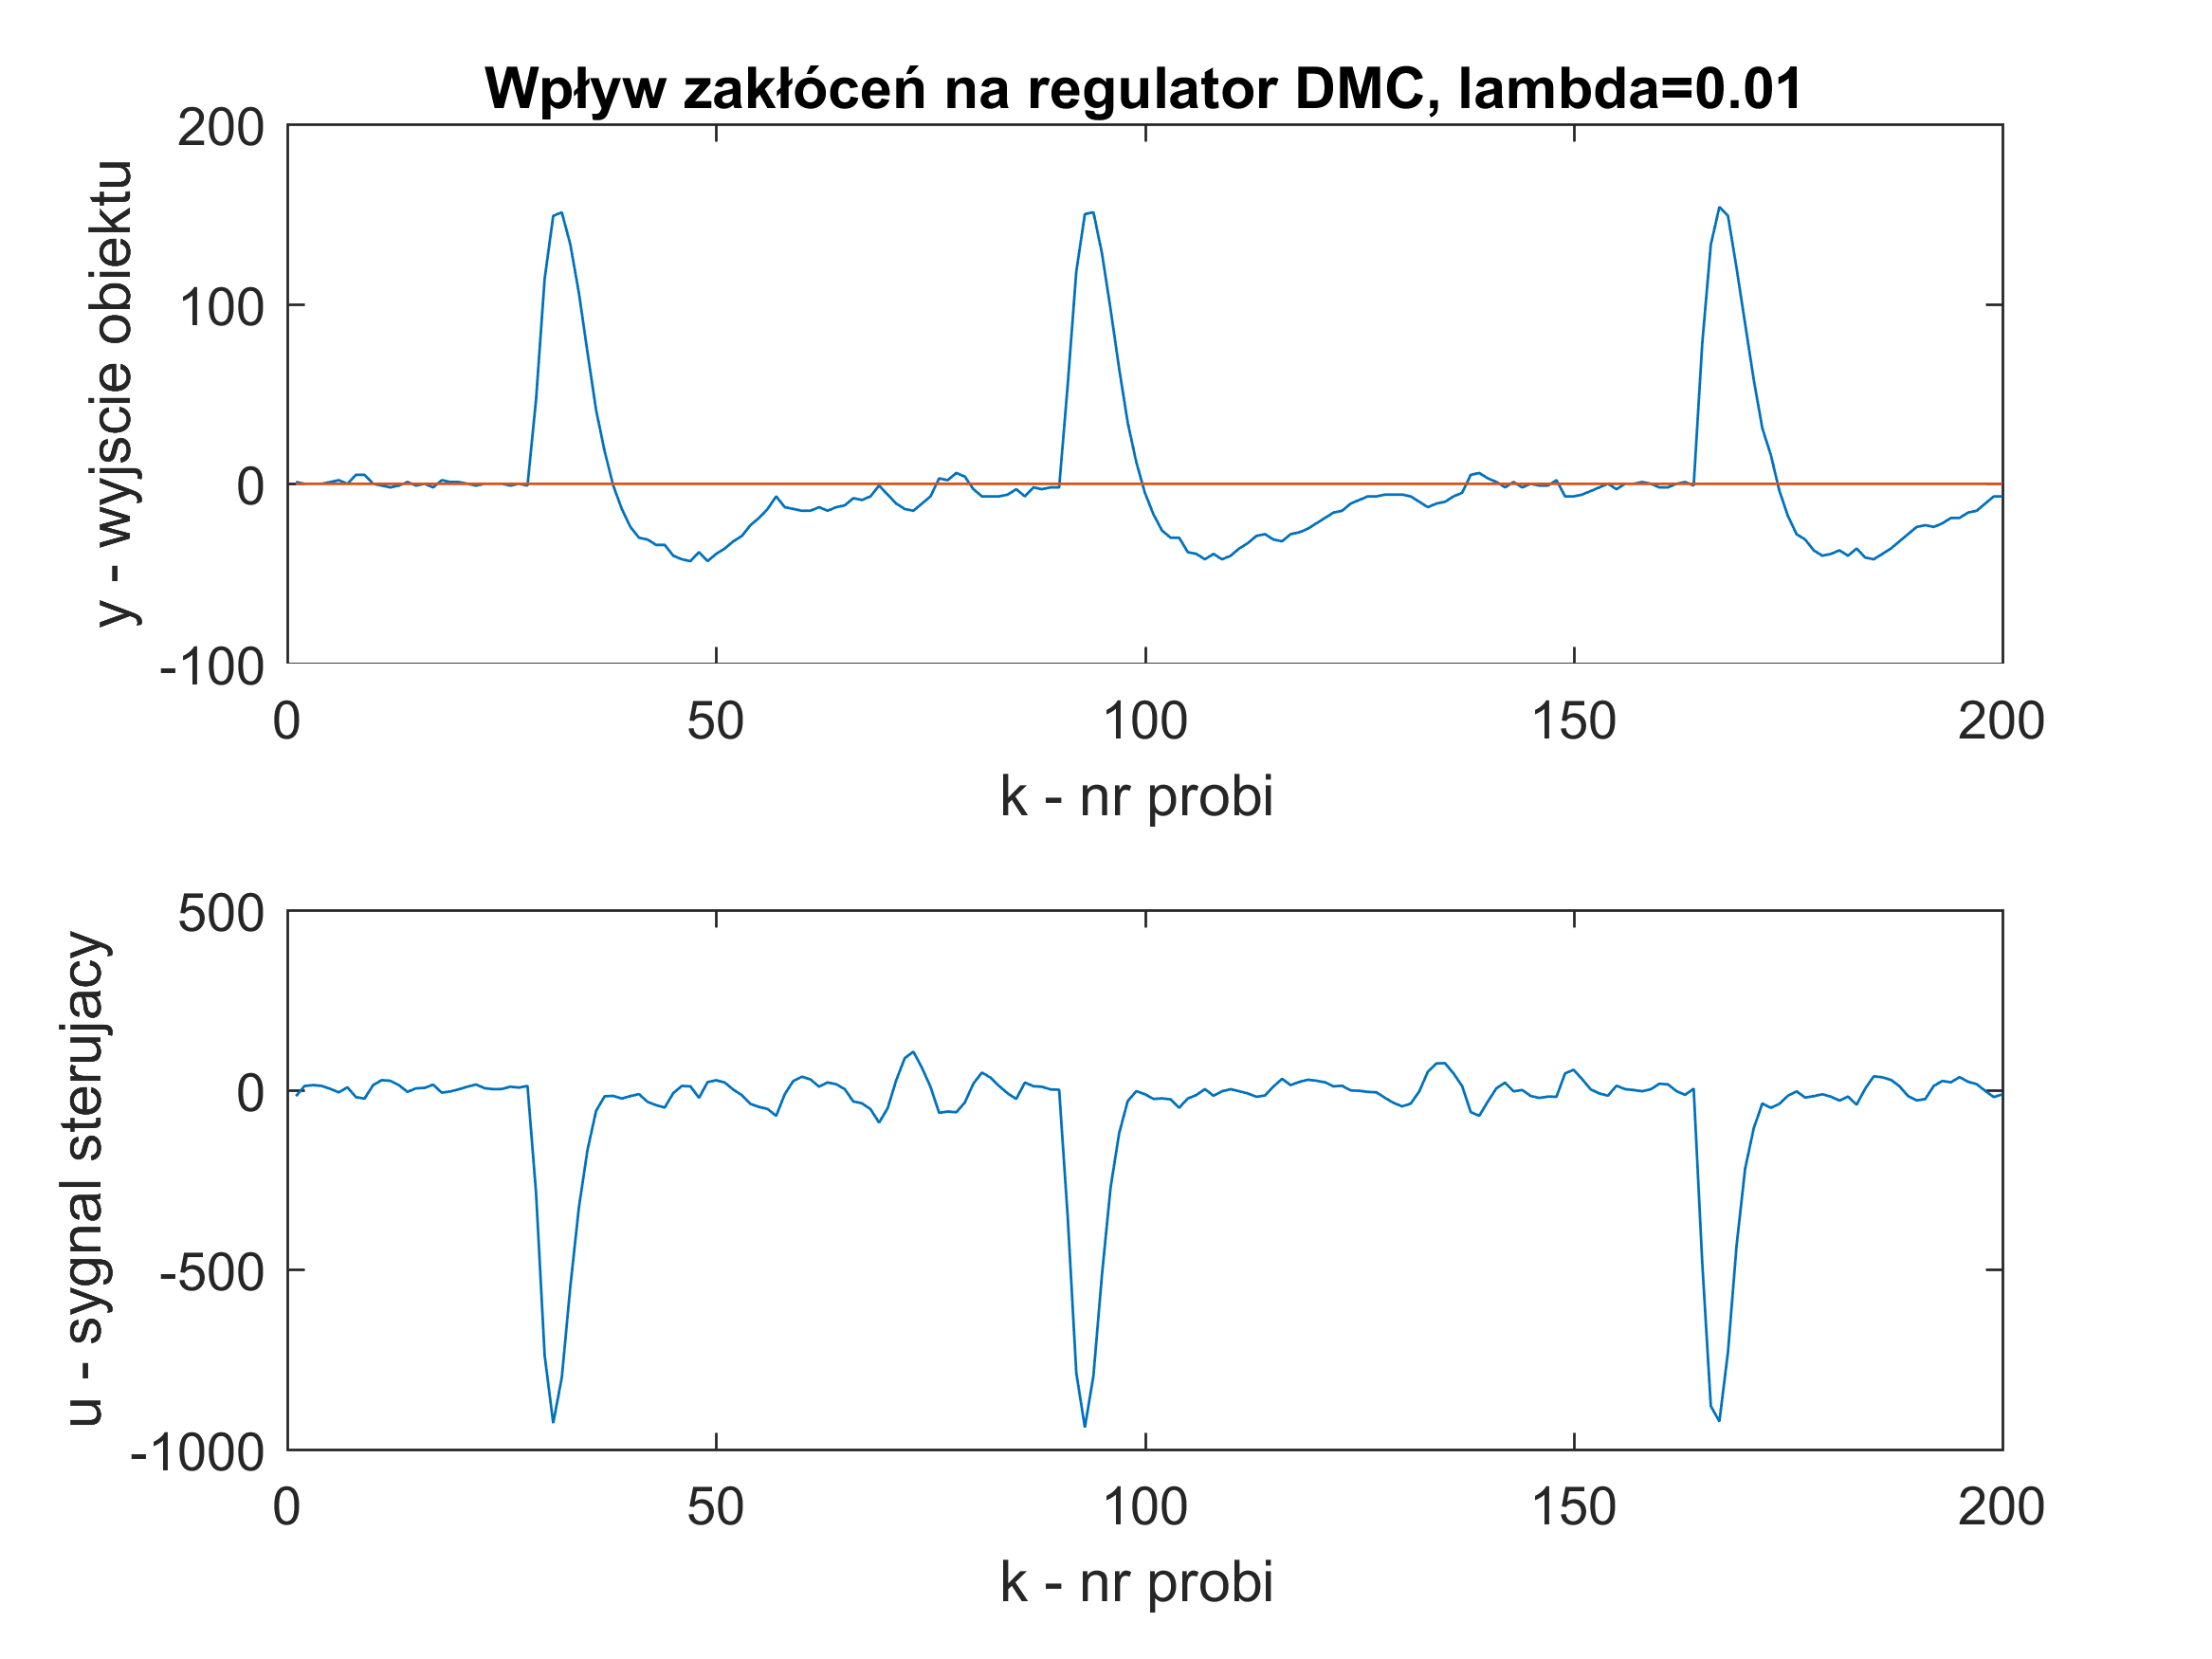
\includegraphics[width=0.9\linewidth]{dmc001zakl}
	\caption{Ocena regulatora DMC: $N=18, N_{u}=7, \lambda=0,01$}
	\label{fig:dmc001zakl}
\end{figure}

\begin{figure}[H]
	\centering
	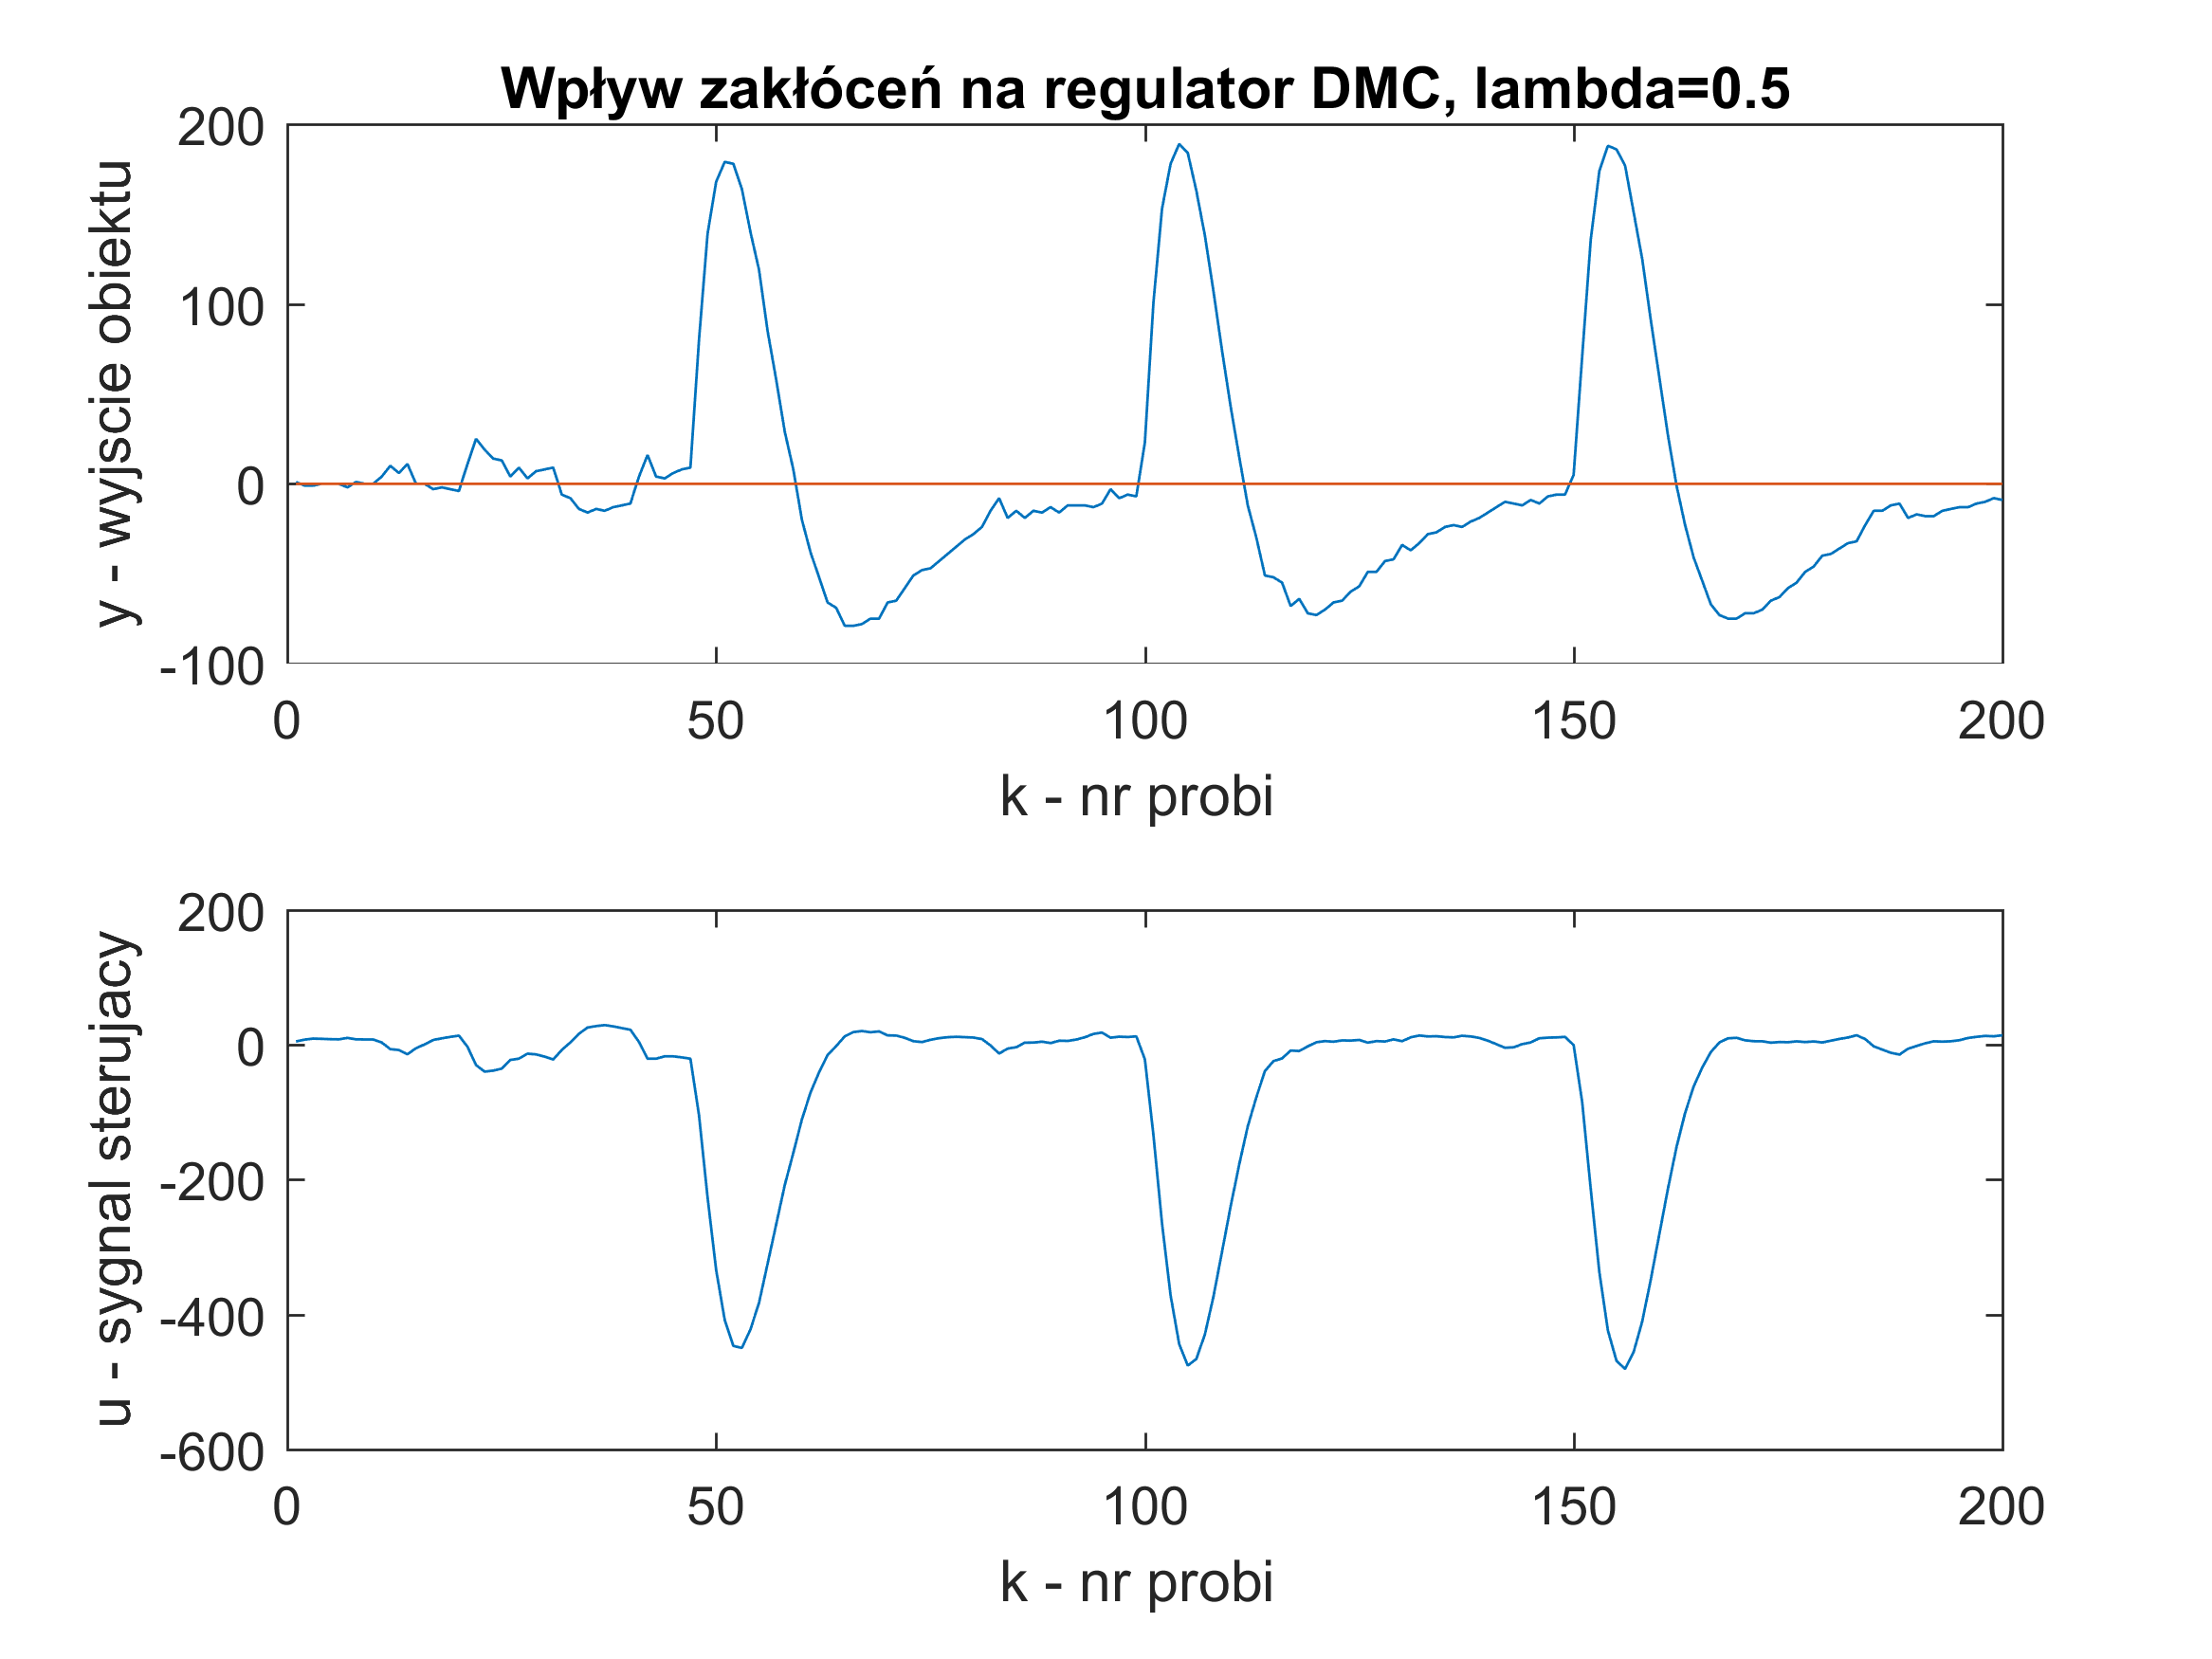
\includegraphics[width=0.9\linewidth]{dmc05zakl}
	\caption{Ocena regulatora DMC: $N=18, N_{u}=7, \lambda=0,5$}
	\label{fig:dmc05zakl}
\end{figure}

\subsection{Przesterowanie}
Przesterowanie dla regulatora PID wyznaczonego metodą inżynierską zostało wyliczone w punkcie \ref{porownaj}. Jest ono równe $3,8\%$ (Rysunek \ref{fig:ocenaPIDMI_przereg1}). Regulator DMC dochodzi do wartości zadanej łagodnie i przesterowanie nie występuje (Rysunek \ref{fig:ocenaDMC_przereg}). Dopiero w dalszych chwilach próbkowania sygnał przekracza bardzo delikatnie wartość zadaną, co jest spowodowane szumami i występuje także dla regulatora PID wyznaczonego metodą inżynerską.

Znaczne przesterowanie występuje dla regulatora PID przy skoku o większą wartość z 500 do -500 (Rysunek \ref{fig:MI_11_}). Dla regulatora DMC dla zmiany wartości zadanej o 1000 przesterowanie także jest zerowe (Rysunek \ref{fig:DMC18750000000_}). 


\begin{figure}[H]
	\centering
	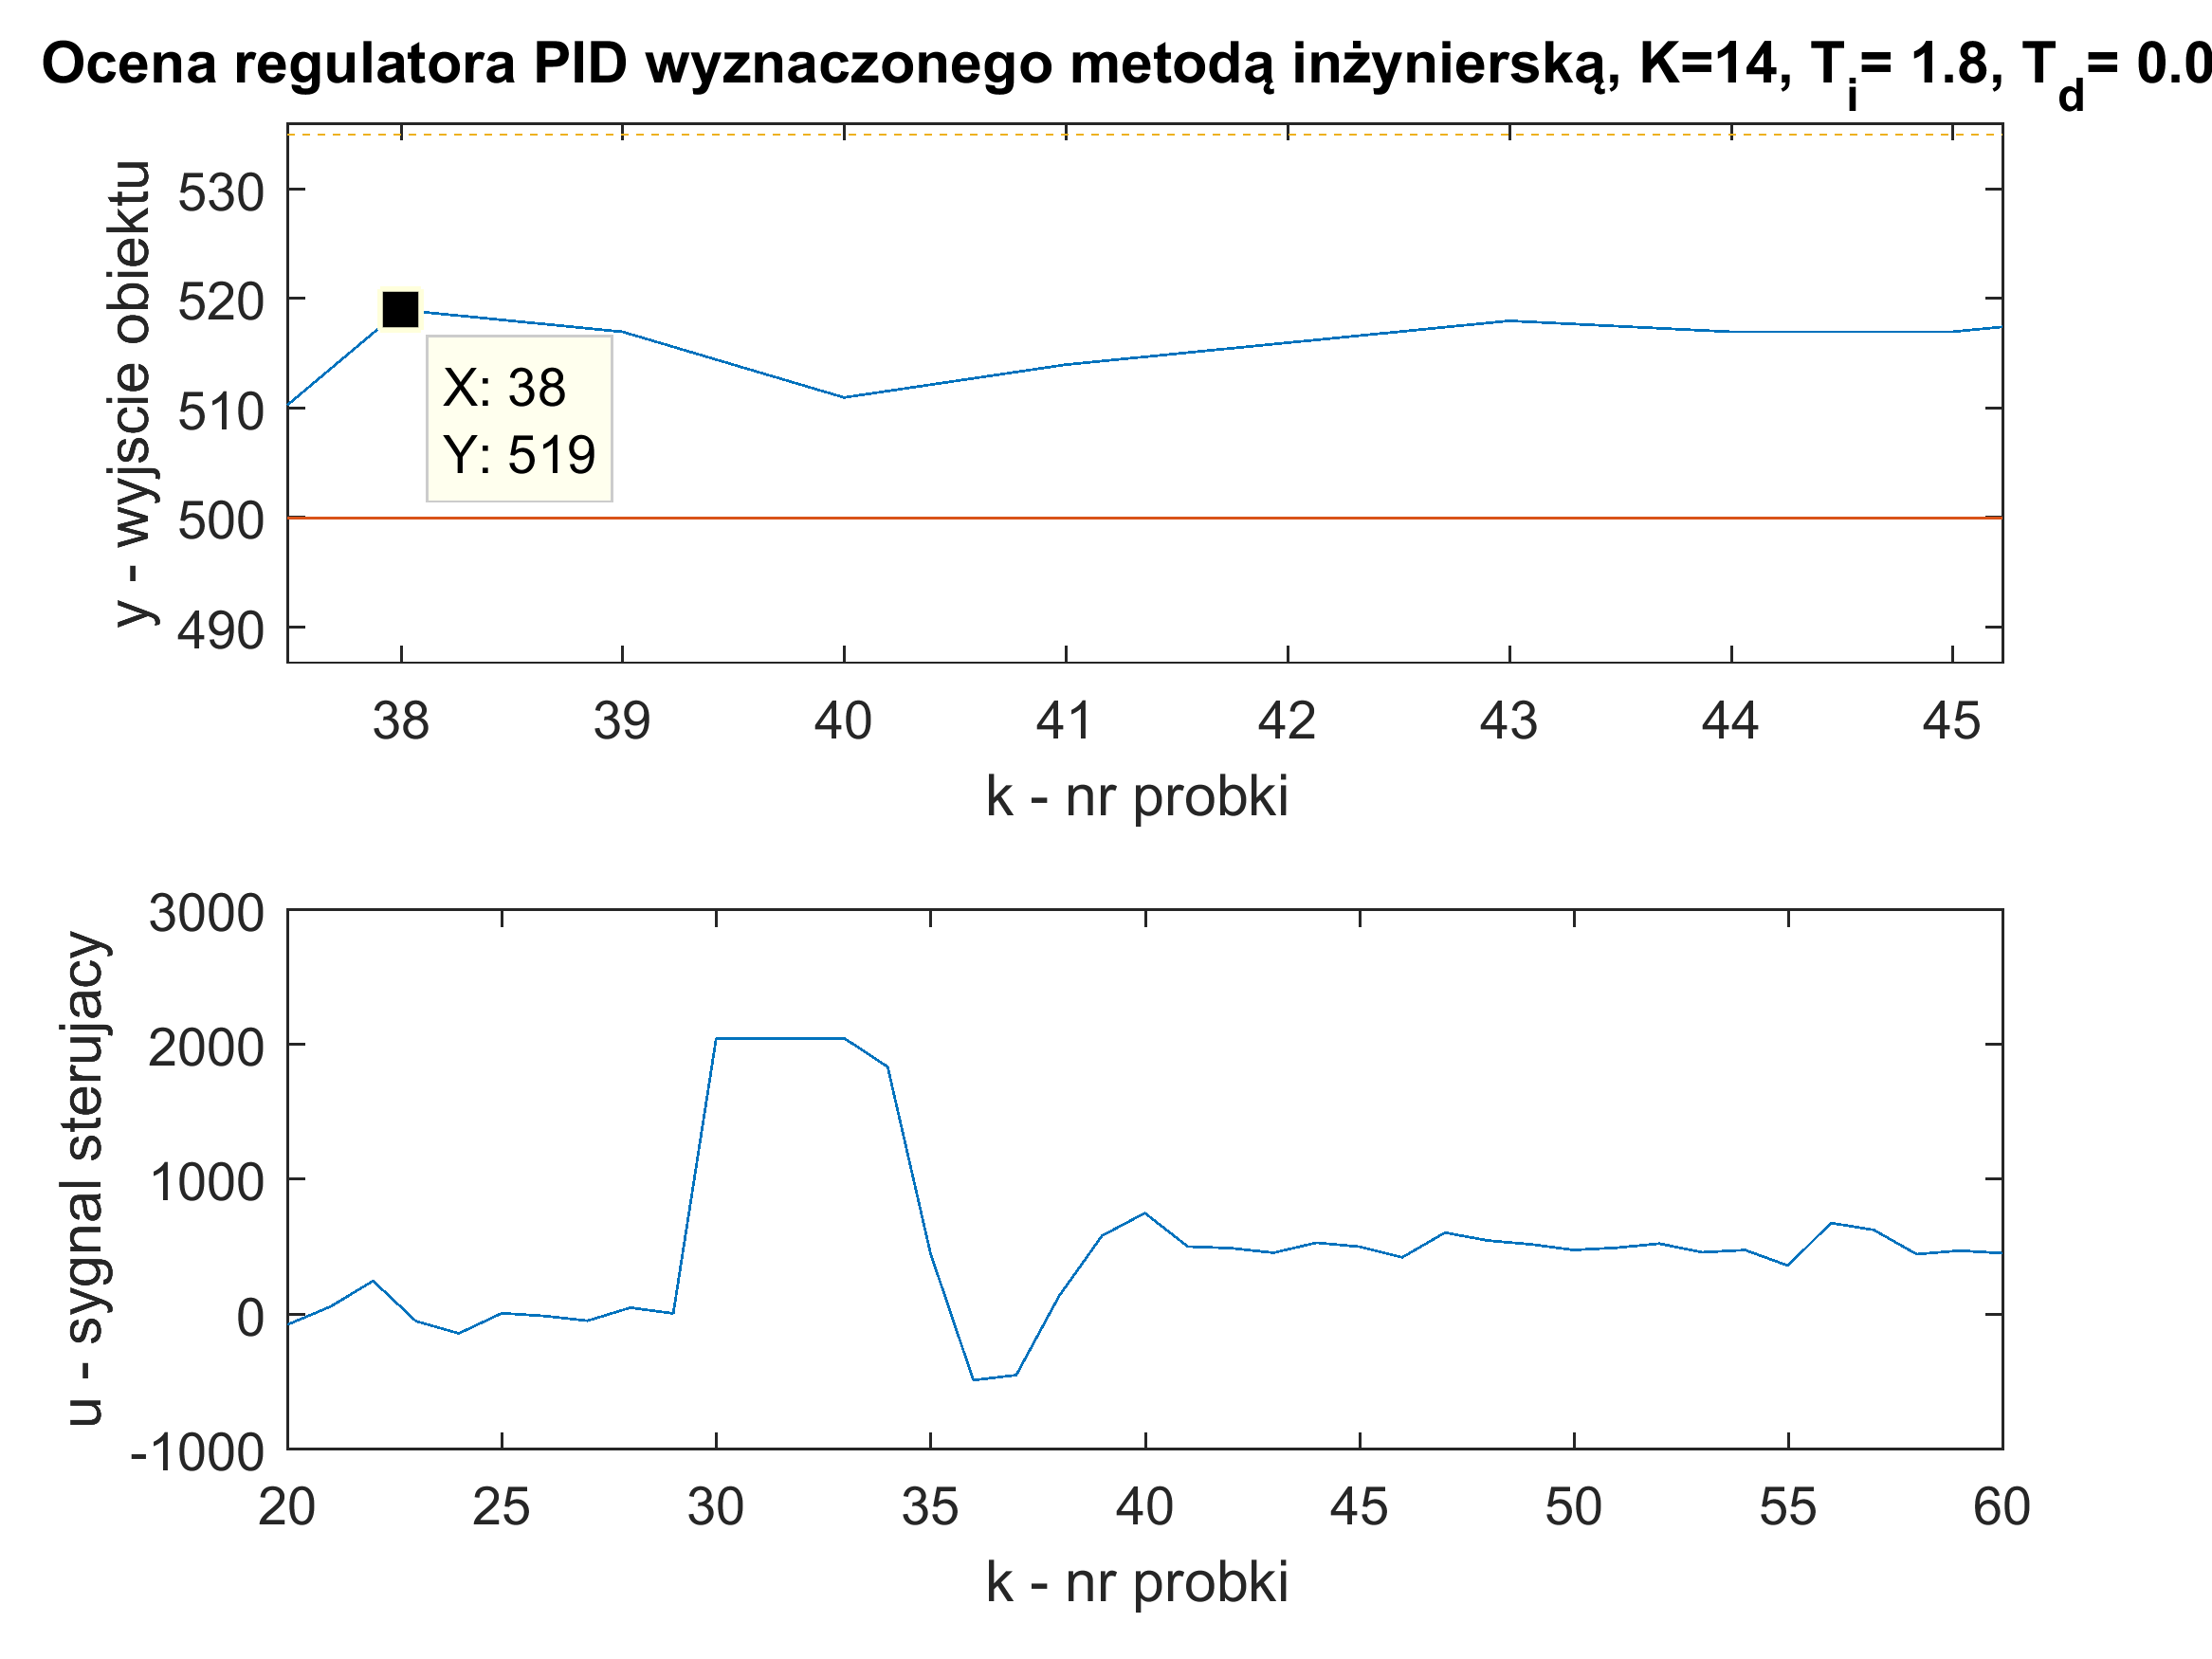
\includegraphics[width=0.9\linewidth]{ocenaPIDMI_przereg}
	\caption{Ocena regulatora PID wyznaczonego metodą inżynierską: $K=14, T_{i}=1,8, T_{d}=0,08$}
	\label{fig:ocenaPIDMI_przereg1}
\end{figure}

\begin{figure}[H]
	\centering
	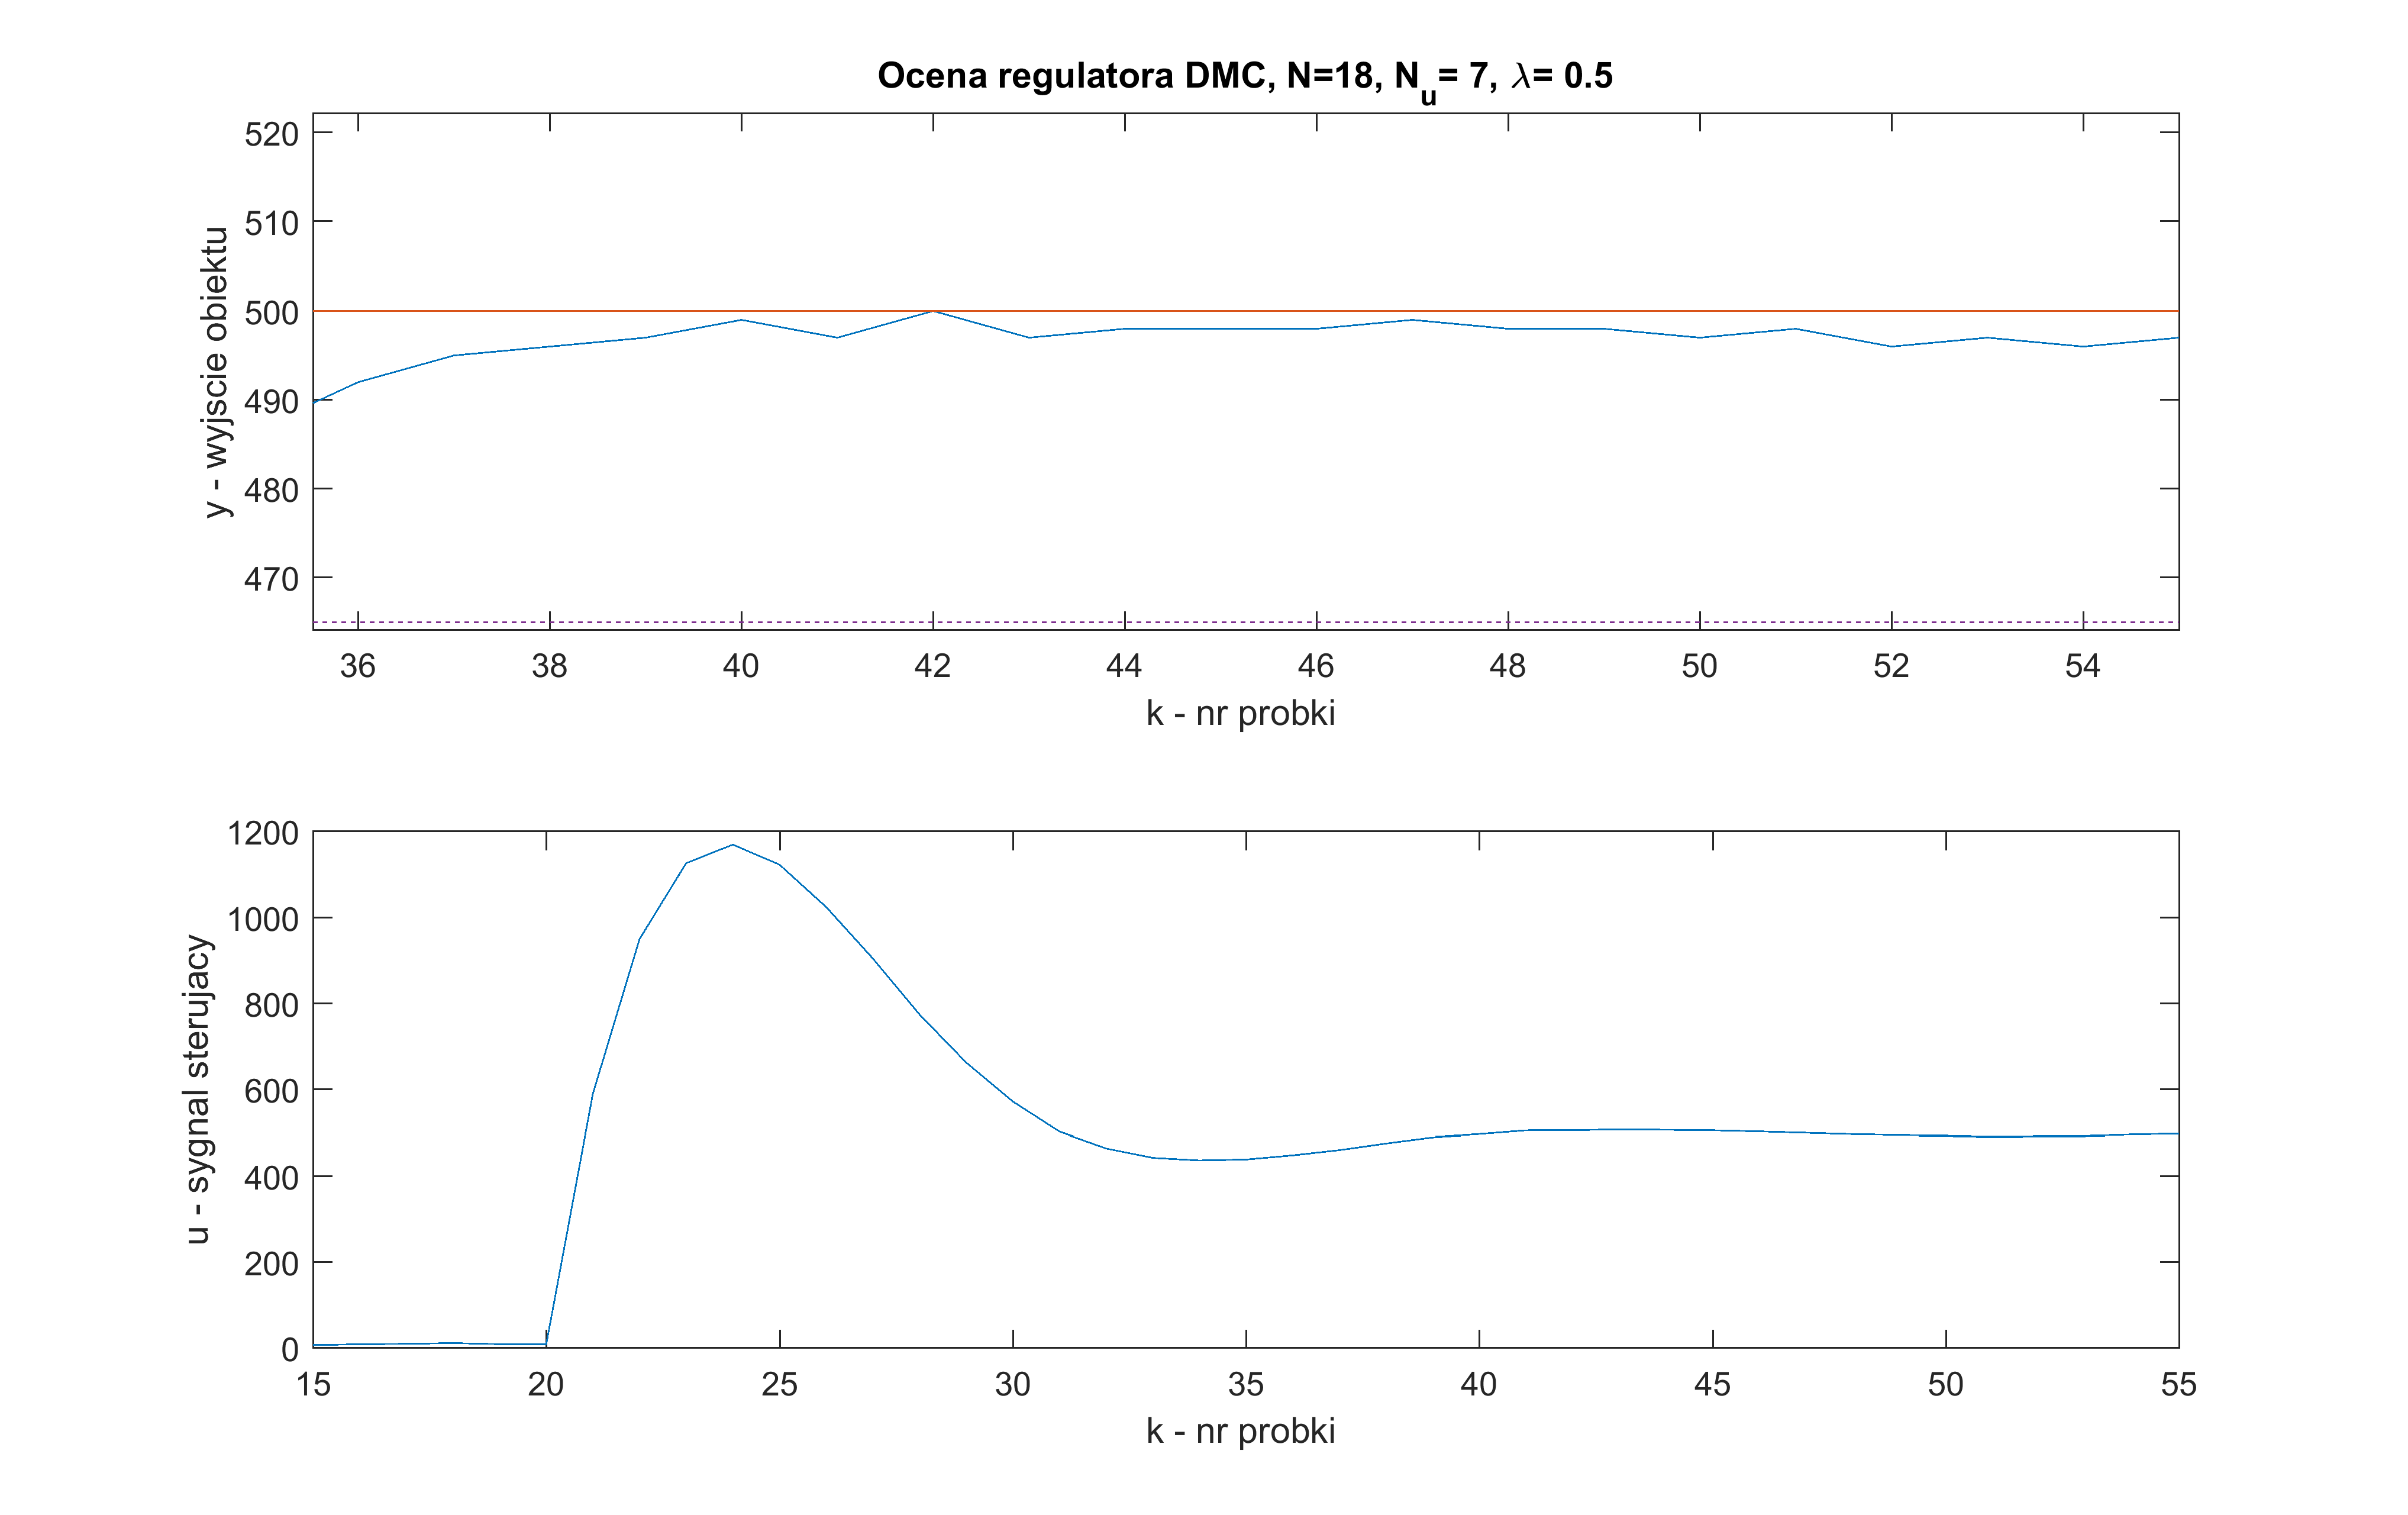
\includegraphics[width=0.9\linewidth]{ocenaDMC_przereg}
	\caption{Ocena regulatora DMC: $N=18, N_{u}=7, \lambda=0,5$}
	\label{fig:ocenaDMC_przereg}
\end{figure}

\subsection{Czas ustalenia}
Dla regulatora PID wyznaczonego metodą inżynierską czas ustalenia został wyliczony w punkcie  \ref{porownaj}. Jest on równy $0,4s$ (Rysunek \ref{fig:ocenaPIDMI1}).
Dla regulatora DMC (Rysunek \ref{fig:ocenaDMC}) wartość zadana sygnału wyjściowego zmienia się w 20 próbce. Próbka 34 jest pierwszą próbką, która wpada w ustalony zakres $y^{zad}-\epsilon$ do $y^{zad}+\epsilon$ i z niego nie wychodzi (dla $\epsilon = 7\% \cdot y^{zad}$). Czas próbkowania jest równy $T=0,05$. Stąd czas ustalenia wynosi $(34-20)\cdot 0,05 = 0,7s$. 
Czas ustalenia jest większy dla regulatora DMC niż dla regulatora PID.

\begin{figure}[H]
	\centering
	\includegraphics[width=0.9\linewidth]{ocenaPIDMI}
	\caption{Ocena regulatora PID wyznaczonego metodą inżynierską: $K=14, T_{i}=1,8, T_{d}=0,08$}
	\label{fig:ocenaPIDMI1}
\end{figure}

\begin{figure}[H]
	\centering
	\includegraphics[width=0.9\linewidth]{ocenaDMC}
	\caption{Ocena regulatora DMC: $N=18, N_{u}=7, \lambda=0,5$}
	\label{fig:ocenaDMC}
\end{figure}

\subsection{Oscylacje}
Dla obu regulatorów występują delikatne oscylacje sygnału wyjściowego po dotarciu do wartości zadanej. Jest to spowodowane szumami i nie da się tego wyeliminować. Przebieg sygnału sterującego jest o wiele łagodniejszy i bez oscylujących zmian dla regulatora DMC, wykres sygnału sterującego dla regulatora PID jest bardziej zmienny.

\begin{figure}[H]
	\centering
	\includegraphics[width=0.9\linewidth]{MI_11}
	\caption{Ocena regulatora PID wyznaczonego metodą inżynierską: $K=14, T_{i}=1,8, T_{d}=0,08$}
	\label{fig:MI_11_}
\end{figure}

\begin{figure}[H]
	\centering
	\includegraphics[width=0.9\linewidth]{DMC18750000000}
	\caption{Ocena regulatora DMC: $N=18, N_{u}=7, \lambda=0,5$}
	\label{fig:DMC18750000000_}
\end{figure}

\section{Wnioski}
\subsection{Wnioski z porównania algorytmów}
Regulator DMC jest lepszy od regulatora PID ze względu na przesterowanie i łagodny przebieg sygnału sterującego. Regulator PID ma krótszy czas ustalenia. Oscylacje sygnału wyjściowego dla obu regulatorów są porównywalne dla stanów ustalonych, dla stanów nieustalonych oscylacje nie występują. Ocena reakcji na zakłócenie zależy od wybranego kryterium. Jeżeli zależy nam na łagodnym przebiegu sygnału sterującego o nie aż tak dużej amplitudzie, należy wybrać regulator DMC. Regulator PID należy wybrać, gdy ważne jest szybki powrót do wartości zadanej i mniejsza amplituda sygnału wyjściowego. Jeszcze lepsze rezultaty można by było uzyskać, gdyby te zakłócenia były mierzalne i uwzględniane w regulacji. Dla regulatora DMC można by było dodać do modelu część odpowiedzialną za zakłócenia. Natomiast do pętli regulacji z regulatorem PID można by było dodać człon odpowiedzialny za redukcję zakłócenia. 

Oceniając regulatory założonymi przez nas kryteriami: \\
- dla obu regulatorów na wyjściu występują delikatne oscylacje (szum) \\
- oba regulatory umożliwiają dotarcie sygnału wyjściowego do zadanej wartości z dokładnością do oscylacji \\
- w obu występuje mniej niż $5\%$ przesterowania, regulator DMC ma mniejsze przesterowanie od PID \\
- czas ustalenia jest krótszy dla regulatora PID.\\
Z naszych założeń wynika, że charakter przebiegu sygnału sterującego nie jest krytyczny, dlatego wybrałybyśmy regulator PID. Umożliwia on szybsze dotarcie do wartości zadanej, ma małe przeregulowanie, znikome oscylacje i  brak uchybu ustalonego.

\subsection{Wnioski ogólne}
W zależności od przyjętych kryteriów można otrzymać regulatory o całkowicie różnym zachowaniu. Trudno stwierdzić, który regulator jest najlepszy, ponieważ jego pożadane cechy zależą od jego celu. W ogólności regulator DMC jest "delikatniejszy" i mniej gwałtowny, m.in. ze wzgledu na karę za zmienny sygnał sterujący. 

Po raz pierwszy spotkałyśmy się z problemem różnego okresu próbkowania sygnału sterującego wychodzącego z regulatora i okresu próbkowania obiektu, co skutkowało specyficznym przebiegiem wyjścia obiektu przy wyznaczaniu wzmocnienia krytycznego i utrudniło to zadanie. 

W naszym przypadku utrudnione było także badanie anty-windupu, ze względu na to, że zmieniałyśmy wartość zadaną w zakresie $<-500,500>$ oraz ze względu na stosunkowo małe znaczenie członu całkującego przy liczeniu sterowania. Z tego powodu anty-windup został zbadany przy innych wartościach zadanych niż  w innych podpunktach. 

Metody przedstawione w projekcie nie są idealne, ponieważ większość doborów parametrów została wykonana \."na oko". Ponadto przy dobieraniu parametrów regulatora PID doprowadziliśmy układ na granicę stabilności, co w przypadku rzeczywistego obiektu mogłoby nie być najlepszym wyborem.





\end{document}
